 
\scchapter{Вводная часть Документации Технологии OSTIS}

\label{chap_intro} 

\begin{SCn}

\scnsectionheader{\currentname}
\scnstartsubstruct

\scsectionbeginningname{Начало Вводной части Документации Технологии OSTIS}
\scnstartsubstruct

\scnheader{\nameref{chap_intro}}
\scnreltovector{конкатенация}{Начало Вводной части Документации Технологии OSTIS;\nameref{foreword};\nameref{intro_ostis};\nameref{intro_lang};\nameref{intro_rules}}
\scnrelfrom{следующий раздел}{\nameref{chap_justification}}

\scntext{аннотация}{\textit{Вводная часть Документации Технологии OSTIS} представляет собой предварительный ответ на следующие вопросы:
\begin{scnitemize}
\item Что такое \textit{Технология OSTIS} (Для чего она предназначена, каковы ее конкурентные преимущества)\char59
\item Что такое \textit{Документация Технологии OSTIS} и как она устроена\char59
\item Что необходимо знать для ознакомления с \textit{Документацией Технологии OSTIS} о стиле и формальных языках, используемых для ее представления.
\end{scnitemize}
}

\scnendstruct

\end{SCn}


\scsection{Предисловие к Документации Технологии OSTIS}
\label{foreword}

\begin{SCn}

\scnsectionheader{\currentname}

\scnstartsubstruct

\bigskip
\scnfilelong{Данная \textit{публикация} посвящена описанию предлагаемой нами \textbf{Технологии OSTIS} (Открытой Семантической Технологии Проектирования Интеллектуальных Компьютерных Систем -- Open Semantic Technology for Intelligent Systems). \textit{Интеллектуальные компьютерные системы}, разработанные на этой технологии, мы назвали \textbf{ostis-системами}. Особенностью \textit{публикации} является то, что она оформлена в виде \uline{внешнего представления} основной части \textit{базы знаний} специальной \textit{ostis-системы}, которая предназначена для комплексной поддержки проектирования \uline{семантически совместимых} \textit{ostis-систем}. Эту систему мы назвали \textbf{\textit{Метасистемой IMS.ostis}} (Intelligent MetaSystem for ostis-systems). Последовательность изложения материала во внешнем представлении \textit{базы знаний} не является единственно возможным маршрутом прочтения (просмотра) \textit{базы знаний}. Каждый читатель, войдя в \textbf{\textit{Метасистему IMS.ostis}}, может выбрать любой другой маршрут навигации по этой \textit{базе знаний}, задавая указанной метасистеме те \textit{вопросы}, которые в текущий момент его интересуют. Таким образом, читая предлагаемый вашему вниманию текст и одновременно работая с \textbf{\textit{Метасистемой IMS.ostis}}, можно значительно быстрее усвоить детали \textbf{\textit{Технологии OSTIS}} и значительно быстрее приступить к непосредственному использованию указанной технологии. Этому также способствует большое количество примеров семантических моделей различных фрагментов \textit{интеллектуальных компьютерных систем}. 

Основной вид \textit{разделов базы знаний \textbf{ostis-системы}} -- это формальное представление различных \textbf{\textit{предметных областей}} вместе с соответствующими им \textbf{\textit{онтологиями}}. При этом явно указываются связи между этими \textbf{\textit{предметными областями} и \textit{онтологиями}}. Таким образом, \textit{база знаний} \textbf{\textit{Метасистемы IMS.ostis}}, как и любых других \textit{интеллектуальных компьютерных систем}, построенных по \textbf{\textit{Технологии OSTIS}}, представляет собой иерархическую систему связанных между собой формальных моделей \textit{предметных областей} и соответствующих им \textit{онтологий}.

В основе \textit{Технологии OSTIS} лежит предлагаемая нами унификация \textit{интеллектуальных компьютерных систем}, основанная, в свою очередь, на \textit{смысловом представлении знаний} в \textit{памяти интеллектуальных компьютерных систем}. Таким образом, данную \textit{публикацию} можно рассматривать как проект \textit{стандарта} семантических моделей \textit{интеллектуальных компьютерных систем}. Последующие \textit{публикации}, посвящённые детальному описанию различных компонентов \textit{Технологии OSTIS}, будут также оформляться как внешнее представление соответствующих \textit{разделов базы знаний} \scnbigspace \textit{Метасистемы IMS.ostis} и будут отражать следующие этапы развития  \textit{Технологии OSTIS}, следующие версии этой технологии, и, соответственно, следующие версии \textit{Метасистемы IMS.ostis}. 

Надеемся на то, что состав авторов таких \textit{публикаций} будет расширяться при четкой спецификации вклада каждого из них. 

Все основные положения \textit{Технологии OSTIS} рассматривались и обсуждались на ежегодных \textit{конференциях OSTIS}, которые стали важным стимулирующим фактором становления и развития \textit{Технологии OSTIS}. Мы благодарим всех активных участников этих конференций.

Важной задачей данной  монографии   была выработка стилистики формализованного представления научно-технической информации, которая одновременно была бы понятна как человеку, так и интеллектуальной компьютерной системе. По сути это принципиально новый подход к оформлению научно-технических результатов, позволяющий:
\begin{scnitemize}
 \item существенно повысить уровень автоматизации анализа качества (корректности, целостности) научно-технической информации;
 \item интеллектуальным компьютерным системам непосредственно (без какой-либо дополнительной “ручной” доработки) использовать информацию (знания)содержащуюся в разработанных специалистами документах;
 \item существенно упростить согласование точек зрения различных специалистов, входящих в коллектив разработчиков той или  иной научно-технической документации.
\end{scnitemize}
Для достижения указанной цели нам было важно привлечь к обсуждению и анализу материала данной монографии как можно больше коллег, участвующих и участвовавших в развитии и применении Технологии OSTIS. При этом некоторых коллег мы включили в число соавторов соответствующих разделов монографии.
Основной целью написания данной монографии является создание технологических и организационных предпосылок к принципиально новому  подходу к организации \textit{научно-технической деятельности} в любой области и, в частности, в области создания и перманентного развития комплексной технологии проектирования и производства семантически совместимых интеллектуальных компьютерных систем (\textit{Технологии OSTIS}). Суть указанного подхода заключается  в глубокой конвергенции и интеграции результатов деятельности всех специалистов, участвующих в создании и развитии \textit{Технологии OSTIS}, путем организации коллективной разработки \textit{базы знаний}, являющейся формальным представлением полной \textit{Документации Технологии OSTIS}, отражающей текущее состояние этой технологии. Для обеспечения высоких темпов и высокого качества данной деятельности мы заинтересованы в расширении контингента участников этой деятельности.

На данном этапе к разработке и оформлению различных разделов Документации по текущей версии \textit{Технологии OSTIS} были привлечены студенты, магистранты, аспиранты и преподаватели кафедры интеллектуальных информационных технологий Белорусского государственного университета информатики и радиоэлектроники и кафедры интеллектуальных информационных технологий Брестского государственного технического университета, а также сотрудники ОАО «Савушкин продукт» и ООО «Интеллектуальные семантические системы». Так, например,
\scnauthorcomment{Добавить соавторов}
\begin{scnitemize}
\item соавторами раздела "" являются ...
\end{scnitemize}
}

\scnheader{ostis-система}
\scnidtf{интеллектуальная компьютерная система, построенная на Технологии OSTIS}
\scnheader{интеллектуальная компьютерная система}
\scnidtf{компьютерная система основанная на знаниях}
\scnheader{база знаний}
\scnidtf{система знаний интеллектуальной компьютерной системы}

\scnendstruct

\end{SCn}

\scsection{Методологические проблемы современного состояния работ в области Искусственного интеллекта}

\label{intro_ostis}

\begin{SCn}

\scnsectionheader{\currentname}

\scnstartsubstruct

\scnsegmentheader{Начало раздела "\currentname"}

\scnstartsubstruct

\scnheader{Методологические проблемы современного состояния работ в области Искусственного интеллекта}

\scnrelfromvector{конкатенация сегментов}
{Структура деятельности в области Искусственного интеллекта;}
\scnauthorcomment{дополнить список}

\scnrelfromset{рассматриваемые вопросы}{
\scnfileitem{Каковы основные стратегические цели (сверхзадачи) научно-технической деятельности в области \textit{Искусственного интеллекта}?};
\scnfileitem{Какие проблемы являются на сегодняшний день актуальными для дальнейшего развития различных направлений \textit{Искусственного интеллекта} и для развития \textit{Искусственного интеллекта} в целом как общей (объединённой) \textit{научно-технической дисциплины}, а также для развития различных форм деятельности в этой области (научно-исследовательской деятельности создания технологий разработки интеллектуальных компьютерных систем, образовательной деятельности, бизнеса)?};
\scnfileitem{Какие проблемы являются на сегодняшний день актуальными для развития других \textit{научно-технических дисциплин} и являются ли эти проблемы аналогичными тем, которые актуальны для развития \textit{Искусственного интеллекта}?};
\scnfileitem{Какие можно предложить подходы к решению указанных выше проблем и как для этого можно использовать создаваемый сейчас новый технологический уклад в области \textit{Искусственного интеллекта} (следующий уровень технологий искусственного интеллекта)?};
\scnfileitem{Как будет выглядеть на основе следующего уровня \textit{технологий Искусственного интеллекта} комплексная автоматизация вех \textit{видов человеческой деятельности}, а также взаимодействие различных \textit{видов человеческой деятельности}, т.е. как будет выглядеть архитектура \textit{smart-общества}?};
\scnfileitem{Устраивает ли нас уровень семантической совместимости взаимопонимания между современными виртуальными компьютерными системами и что необходимо сделать для повышения этого уровня?};
\scnfileitem{Устраивает ли нас уровень семантической совместимости взаимопонимания между современными интеллектуальными компьютерными системами их пользователями и что необходимо сделать для повышения этого уровня?}}
\scntext{аннотация}{Предлагаемое вашему вниманию рассмотрение методологических проблем современного состояния работ в области \textit{Искусственного интеллекта} состоит из следующих частей:
\begin{scnitemize}
\item Анализ актуальных проблем, препятствующих дальнейшему развитию  \textit{Искусственного интеллекта} как \textit{научно-технической дисциплины}:
\begin{scnitemizeii}
\item Проблемы развития научных исследований в области \textit{Искусственного интеллекта} 
\item Проблемы разработки технологий проектирования и реализации \textit{интеллектуальных компьютерных систем};
\item Проблемы формирования рынка \textit{интеллектуальных компьютерных систем}; 
\item Образовательные проблемы в области \textit{Искусственного интеллекта};
\item Проблемы развития бизнеса в области \textit{Искусственного интеллекта}.
\end{scnitemizeii}
\item Анализ проблем автоматизации сложных видов деятельности:
\begin{scnitemizeii}
\item научно-исследовательской деятельности в рамках различных научных дисциплин;
\item создание \textit{технологий проектирования} и производства (реализации) сложных технических систем;
\item \textit{инженерной деятельности} по разработке сложных технических систем;
\item \textit{образовательной деятельности} по наукоёмким техническим специальностям
\end{scnitemizeii}
\item Формулировка принципов, лежащих в основе \textit{Технологии OSTIS}, предназначенной для решения указанных выше проблем;
\item Рассмотрение структуры \textit{Экосистемы OSTIS}, построенной по \textit{Технологии OSTIS} и обеспечивающей комплексную автоматизацию всех видов человеческой деятельности
\end{scnitemize}}

\scnrelfromset{используемые знаки общих понятий и иных сущностей}{деятельность\\
\scnaddlevel{1}
\scnidtf{область деятельности}
\scnsuperset{человеческая деятельность}
\scnaddlevel{-1}
;вид деятельности\\
\scnaddlevel{1}
\scnhaselement{проектирование}
\scnaddlevel{1}
\scnidtf{проектная деятельность}
\scnaddlevel{-1}
\scnhaselement{производство}
\scnaddlevel{1}
\scnidtf{производственная деятельность}
\scnaddlevel{-1}
\scnhaselement{наука}
\scnaddlevel{1}
\scnidtf{научная деятельность}
\scnaddlevel{-2}
;проект\\
\scnaddlevel{1}
\scnsuperset{открытый проект}
\scnaddlevel{-1}
;консорциум
;технология\\
\scnaddlevel{1}
\scnsuperset{информационная технология}
\scnaddlevel{1}
\scnsuperset{технология искусственного интеллекта}
\scnaddlevel{-2}
;кибернетическая система\\
\scnaddlevel{1}
\scnsuperset{интеллектуальная система}
\scnaddlevel{1}
\scnsuperset{интеллектуальная компьютерная система}
\scnaddlevel{1}
\scnidtf{искусственная интеллектуальная система}
\scnaddlevel{-3}
;конвергенция\scnsupergroupsign
\scnaddlevel{1}
\scnidtf{уровень конвергенции (близости)}
\scnsuperset{конвергенция кибернетических систем\scnsupergroupsign}
\scnaddlevel{-1}
;интеграция*\\
\scnaddlevel{1}
\scnsuperset{интеграция кибернетических систем*}
\scnsuperset{эклектичная интеграция*}
\scnsuperset{глубокая интеграция*}
\scnaddlevel{-1}
;интегрированная система\\
\scnaddlevel{1}
\scnsuperset{эклектичная система}
\scnsuperset{гибридная система}
\scnaddlevel{-1}
;экосистема интеллектуальных компьютерных систем
;рынок знаний\\
\scnaddlevel{1}
\scnidtf{рыночная организация порождения эволюции и применения знаний}
\scnaddlevel{-1}
;smart-общество\\
\scnaddlevel{1}
\scnidtf{общество,в основе которого лежит экосистема интеллектуальных компьютерных систем и рынок знаний}
\scnaddlevel{-1}
}
 
\scnrelfromset{ключевые знаки}
{Искусственный интеллект\\
\scnaddlevel{1}
\scniselement{научно-техническая дисциплина}
\scnaddlevel{1}
\scnsubset{научно-техническая деятельность} 
\scnaddlevel{-2};
интеллектуальная система\\
\scnaddlevel{1}
\scnsuperset{интеллектуальная компьютерная система}
\scnaddlevel{-1};
Общая теория интеллектуальных систем;
Базовая комплексная технология проектирования интеллектуальных компьютерных систем;
Технология производства спроектированных интеллектуальных компьютерных систем;
Специализированная инженерия в области Искусственного интеллекта;
Образовательная деятельность в области Искусственного интеллекта;
Бизнес-деятельность в области Искусственного интеллекта\bigskip;
\scnkeyword{Технология OSTIS};
\scnkeyword{ostis-система};
смысловое преставление информации;
агентно-ориентированная модель обработки информации в памяти; стандартизация ostis-систем;
\scnkeyword{SC-код};
абстрактная sc-машина;
конвергенция знаний в памяти;
ostis-систем;
конвергенция моделей решения задач в  ostis-системе;
интеграция знаний в памяти  ostis-системы;
интеграция моделей решения задач в  ostis-системе;
ostis-сообщество;
ostis-технология\\
\scnaddlevel{1}
\scnsuperset{ostis-технология проектирования}
\scnsuperset{ostis-технология производства}
\scnsuperset{технология эксплуатации ostis-систем}
\scnsuperset{технология реинжиниринга ostis-систем}
\scnaddlevel{-1};
\scnkeyword{Ядро Технологии OSTIS}\bigskip;
OSTIS-портал научных знаний в области Искусственного интеллекта;
Проект IMS.ostis;
\scnkeyword{Метасистема IMS.ostis};
Проект Программной реализации универсальной абстрактной sc-машины;
Проект разработки Универсального sc-компьютера;
Специализированная инженерия, осуществляемая на основе Технологии OSTIS;
Образовательная деятельность в области Искусственного интеллекта, осуществляемая на основе технологии OSTIS;
\scnkeyword{Консорциум OSTIS}\bigskip;
\scnkeyword{Экосистема OSTIS};
человеческая деятельность;
вид человеческой деятельности;
автоматизация человеческой деятельности;
качество человеческой деятельности;
субъект Экосистемы OSTIS;
Рынок знаний, реализованный в рамках Экосистемы OSTIS;
smart-общество}

\scnendstruct


\newpage
\begin{SCn}
	\scnsegmentheader{Структура Деятельности в области Искусственного интеллекта}
	
	\scntext{аннотация}{Для того, чтобы рассмотреть проблемы дальнейшего развития \textit{деятельности} в области \textit{Искусственного интеллекта} как \textit{научно-технической дисциплины} и, в частности, проблемы комплексной автоматизации этой \textit{деятельности}, необходимо уточнить структуру указанной \textit{деятельности}.
	}
	
	\scnheader{Искусственный интеллект}
	\scniselement{область человеческой деятельности}
	\scniselement{научно-техническая дисциплина}
	\scnaddlevel{1}
	\scniselement{вид человеческой деятельности}
	\scnaddlevel{-1}
	\scnidtf{Область человеческой деятельности, основными целями которой являются:
		
		\begin{scnitemize}
			\item построение теории  интеллектуальных систем;
			\item создание  технологии разработки интеллектуальных компьютерных систем (искусственных интеллектуальных систем);
			\item переход на принципиально новый уровень комплексной автоматизации всех \textit{видов человеческой деятельности}, который основан на массовом применение \textit{интеллектуальных    компьютерных систем} и который предполагает:
			\begin{scnitemizeii}
				\item не только наличие \textit{интеллектуальных компьютерных систем}, способных понимать друг друга и согласовывать свою деятельность,
				\item но и построение \textit{общей теории  человеческой деятельности},  осуществляемый в условиях нового уровня её автоматизации, ( теории деятельности \textit{smart-общества}), которая должна быть "  понятна" \textit{используемым интеллектуальным компьютерным системам} и которая потребует существенного переосмысления современной организации \textit{человеческой деятельности}.
			\end{scnitemizeii}
		\end{scnitemize}
	}
	
	
	\scnheader{Искусственный интеллект}
	\scnidtf{Научно-техническая деятельность, направленная на построение теории интеллектуальных систем, а также на создание технологии проектирования и производства  искусственных интеллектуальных систем (\textit{интеллектуальных компьютерных систем})}
	\scnidtf{Научно-техническая деятельность в области \textit{Искусственного интеллекта}}
	\scnidtf{Деятельность в области \textit{Искусственного интеллекта}}
	
	\scnidtf{Научно-техническая деятельность, направленная на исследование феномена \textit{интеллекта}, а также на создание искусственных интеллектуальных систем( \textit{интеллектуальных компьютерных систем}) и включающая в себя соответствующую научно-исследовательскую деятельность, инженерно-технологическую, инженерно-прикладную, образовательную и организационную деятельность}
	
	\scnexplanation{Междисциплинарная (трансдисциплинарная) область \textit{научно-технической деятельности}, направленная на разработку и эксплуатацию \textit{интеллектуальных  компьютерных систем},  обеспечивающих автоматизацию различных сфер \textit{человеческой деятельности}.}
	
	\scnidtf{Научно-техническая дисциплина направленная на разработку теории индивидуальных \textit{интеллектуальных компьютерных систем} и \textit{интеллектуальных сообществ} (коллективов) таких систем, а также средств поддержки их проектирования и реализации)}
	
	\scnidtf{\textit{Научно-техническая  дисциплина}, являющаяся частью \textit{кибернетики} (теория кибернетических систем), объектом исследования которой являются  \textit{интеллектуальные компьютерные системы}  (искусственные \textit{интеллектуальные системы})и  целями которой являются
		(1) разработка \textit{теории интеллектуальных компьютерных систем}, 
		(2) разработка \textit{технологии(методов и средств)} \textit{проектирования и производства компьютерных систем}, а также,
		(3)разработка конкретных интеллектуальных компьютерных систем различного назначения.}
	
	
	\scnheader{Искусственный интеллект}
	\scnrelfrom{декомпозиция}{Декомпозиция Искусственного интеллекта по формам деятельности}
	\scnaddlevel{1}
	
	
	
	\scneqtoset{Научно-исследовательская деятельность в области Искусственного интеллекта\\
		\scnaddlevel{1}
		\scnrelfrom{продукт}{Общая теория интеллектуальных систем}
		\scnaddlevel{1}
		\scnidtf{Теория, уточняющая структуру и принципы функционирования \textit{интеллектуальных систем}, а также акцентирующая внимание на причинах (предпосылках) возникновение свойства интеллектуальности (феномены \textit{интеллекта})}
		\scnaddlevel{-1}
		\scniselement{коллективная научно-техническая деятельность}
		\scnaddlevel{1}
		\scniselement{вид человеческой деятельности}
		\scnidtf{научно-исследовательская дисциплина или направление} 
		\scnrelboth{следует отличать}{продукт научно-исследовательской деятельности}
		\scnaddlevel{-2};
		Разработка Базовой комплексной технологии проектирования интеллектуальных компьютерных систем\\
		\scnaddlevel{1}
		\scnrelfrom{продукт}{Базовая комплексная технология проектирования интеллектуальных компьютерных систем}
		\scnaddlevel{1}
		\scnnote{Комплексность данной \textit{технологии}  заключается в том, что она ориентирована
			(1) на проектирование \textit{интеллектуальных компьютерных систем} в целом, а не только отдельных их компонентов и
			(2) на создание объединённой \textit{технологии}, объединяющей самые различные технологические подходы на основе их  \textit{конвергенции} и глубокой  \textit{интеграции}}
		\scnaddlevel{-1}
		\scniselement{разработка технологии проектирования искусственных объектов заданного класса}
		\scnaddlevel{1}
		\scniselement{вид человеческой деятельности}
		\scnaddlevel{-2};
		Разработка Технологии производства спроектированных интеллектуальных компьютерных систем\\
		\scnaddlevel{1}
		\scnrelfrom{продукт}{Технология производства спроектированных интеллектуальных компьютерных систем}
		\scnaddlevel{1}
		\scnidtf{технология реализации (сборки и установки) спроектированных интеллектуальных компьютерных систем}
		\scnnote{Очевидно, что данная \textit{технология} должна быть самым тесным образом связана с \textit{Базовой комплексной технологией проектирования интеллектуальных компьютерных систем} (по крайней мере данная \textit{технология}  должна "знать", какой форме ей на "вход" передаётся результат проектирования). Поэтому имеет смысл говорить об объединённой технологии проектирования и производства \textit{интеллектуальных компьютерных систем}}
		\scnaddlevel{-1}
		\scniselement{производства спроектированных искусственных объектов заданного класса}
		\scnaddlevel{1}
		\scniselement{вид человеческой деятельности}
		\scnaddlevel{-2};
		Специализированная инженерия в области Искусственного интеллекта\\
		\scnaddlevel{1}
		\scnidtf{Множество Процессов разработки (проектирования и производства)  \textit{интеллектуальных компьютерных систем} различного назначения, кроме \textit{интеллектуальных компьютерных систем автоматизации проектирования} и автоматизации производства \textit{интеллектуальных компьютерных систем}}
		\scnrelfrom{продукт}{множество специализированных интеллектуальных компьютерных систем}
		\scnaddlevel{1}
		\scnrelfrom{основной sc-идентификатор*}{прикладная интеллектуальная компьютерная система}
		\scnaddlevel{-1}
		\scnsubset{проектирование и производство искусственного объекта заданного класса на основе заданной технологии}
		\scnaddlevel{1}
		\scniselement{вид человеческой деятельности}
		\scnaddlevel{-2};
		Образовательная деятельность в области Искусственного интеллекта\\
		\scnaddlevel{1}
		\scnidtf{Деятельность, направленная на подготовку молодых специалистов области \textit{Искусственного интеллекта} на перманентное повышение квалификации действующих специалистов в этой области}
		\scnnote{Сложность и высокая степень наукоемкости задач, больших своего решения на текущем этапе развития \textit{Искусственного интеллекта}, добавляют к специалистам, работающим в этой области высокие требования к уровню их:
			\begin{scnitemize}
				\item математической культуры (культуры формализации) ;
				\item системной культуры;
				\item технологической культуры;
				\item инженерная культура;
				\item умения работать коллективных наукоемких процесс проектах.
			\end{scnitemize}
		}
		\scnaddlevel{-1}
		\scnsubset{образовательная деятельность}
		\scnaddlevel{1}
		\scniselement{вид человеческой деятельности}
		\scnaddlevel{-1};
		Бизнес деятельность в области искусственного интеллекта\\
		\scnaddlevel{1}
		\scnexplanation{Речь идет о бизнес-деятельности в широком смысле как деятельности, направленный на создание  инфраструктурных условий для качественного выполнения всех \textit{видов деятельности} в области \textit{Искусственного интеллекта}, а именно:
			\begin{scnitemize}
				\item на разработку и реализацию грамотной научно-технической политики, связывающей как тактические, так и стратегические цели;
				\item на глубокую \textit{конвергенцию} всех форм и \textit{видов деятельности} в области \textit{Искусственного интеллекта};
				\item на организацию взаимовыгодного сотрудничество различных школ и коллективов, работающих в области \textit{Искусственного интеллекта};
				\item на финансовое обеспечение;
				\item на кадровое обеспечение;
				\item на материально-техническое обеспечение;
				\item на организацию проведения различных мероприятий (конференций, выставок, семинаров);
				\item на публикационную деятельность и защиту интеллектуальной собственности;
				\item на материально-техническое обеспечение;
			\end{scnitemize}
		}
		\scnsubset{бизнес-деятельность научно-технической области}
		\scnaddlevel{1}
		\scniselement{вид человеческой деятельности}
		\scnaddlevel{-2}
	}
	
	\scnheader{Разработка базовой комплексной технологии проектирования интеллектуальных компьютерных систем}
	\scnrelfromset{декомпозиция}{Разработка общей теории интеллектуальных компьютерных систем\\
		\scnaddlevel{1}  
		\scnrelfrom{продукт}{Общая теория интеллектуальных компьютерных систем}
		\scniselement{разработка теории искусственных объектов заданного класса}
		\scnaddlevel{1}
		\scniselement{вид человеческой деятельности}
		\scnaddlevel{-2}
		;Разработка общей теории интеллектуальных компьютерных систем\\
		\scnaddlevel{1}
		\scnrelfrom{продукт}{Теория проектирования интеллектуальных компьютерных систем}
		\scnaddlevel{1}
		\scnnote{В состав этой теории входят методы проектирования, библиотеки проектирования и спецификация используемых индустриальных средств.}
		\scnaddlevel{-1}
		\scnidtf{Разработка \textit{Теории проектной деятельности} по построению формальных моделей \textit{интеллектуальных компьютерных систем}}
		\scniselement{теории проектирования интеллектуальных объектов заданного класса}
		\scnaddlevel{1}
		\scniselement{вид человеческой деятельности}
		\scnaddlevel{-2};
		Разработка комплекса средств автоматизации проектирования интеллектуальных компьютерных систем\\
		\scnaddlevel{1}
		\scniselement{разработка комплекса средств автоматизации проектирования искусственных объектов заданного класса}
		\scnaddlevel{1}
		\scniselement{вид человеческой деятельности}
		\scnaddlevel{-2}
	}
	
	\scnheader{Разработка Технологии производства спроектированных интеллектуальных компьютерных систем}
	\scnrelfromset{декомпозиция}{Разработка Теории производства спроектированных интеллектуальных компьютерных систем\\
		\scnaddlevel{1}  
		\scnidtf{Разработка \textit{Теории производственной деятельности} по реализации (сборке и установке) \textit{интеллектуальных компьютерных систем}}
		\scnrelfrom{продукт}{Теория производства спроектированных интеллектуальных компьютерных систем}
		\scnaddlevel{1}
		\scnnote{В состав этой \textit{теории} входят \textit{методы производства} (сборки и установки) \textit{интеллектуальных компьютерных систем}, а также спецификация \textit{используемых инструментальных средств}.}
		\scnaddlevel{-2}
		;Разработка комплекса средств автоматизации производства интеллектуальных компьютерных систем\\
		\scnaddlevel{1}
		\scniselement{разработка комплекса средств автоматизации производства искусственных объектов заданного класса}
		\scnaddlevel{1}
		\scniselement{вид человеческой деятельности}
		\scnaddlevel{-2}
	}
	
	\scnheader{Специализированная инженерия в области Искусственного интеллекта}
	\scnidtf{проектирование и производство конкретной \textit{интеллектуальной компьютерной системы} по заданной технологии}  
	\scnrelfromset{обобщенная декомпозиция}{проектирование конкретные интеллектуальные компьютерные системы\\
		\scnaddlevel{1}
		\scnrelfromset{обобщенное разбиение}{проектирование интеллектуальной компьютерной системы автоматизации проектирования соответствующего класса интеллектуальных компьютерных систем; проектирование интеллектуальной компьютерной системы автоматизации проектирования соответствующего класса объектов, не являющихся интеллектуальными компьютерными системами; проектирование интеллектуальной компьютерной системы,не являющейся системой автоматизации проектирования
		}
		\scnaddlevel{-1}
		;производство конкретной спроектированной интеллектуальной компьютерной системы\\
	}
	
	\scnheader{Производство конкретной спроектированной интеллектуальной компьютерной системы}
	\scnnote{Производственная деятельность направленная на \textit{производство} (реализацию) спроектированной \textit{интеллектуальной компьютерной системы} значительно уступает по уровню сложности деятельности проектированию этой \textit{интеллектуальной компьютерной системы}, так как это производство сводится к сборке результата \textit{проектирования} (формальной логико-семантической модели разрабатываемой \textit{интеллектуальной компьютерной системы}) и загрузки этой модели в память компьютера или программного \textit{универсального интерпретатора логико-семантических моделей интеллектуальных компьютерных систем}, в качестве которого может быть использован
		(1) либо специально разработанный для этого \textit{компьютер}, ориентированные на обработку \textit{баз знаний} и интерпретацию различных \textit{интеллектуальных моделей решения задач},
		(2) либо программная эмуляция такого \textit{компьютера}, реализованная на современных  \textit{компьютерах} фон-неймановской архитектуры.
		
		Простота производства спроектированных систем характерна для производства не только интеллектуальных, но и любых других \textit{компьютерных систем}.
		
		Мы выделяем "производственный" этап реализации \textit{интеллектуальных компьютерных систем} для того, чтобы по аналогии рассматривать этап производства (массового, мелкосерийного, разового производства) спроектированных искусственных объектов любого другого вида(микросхем, автомобилей, зданий,  компьютеров).
		
		Очевидно, что массовое производство некоторых видов продукции может иметь весьма большой уровень сложности, но при этом суть \textit{производственной деятельности} как процесса перехода от проекта (спецификации) некоторого объекта к его реализации остаётся одной и той же независимо от уровня сложности  реализуемого объекта (производимой продукции).
	}	
	\scnaddlevel{-1}	
	\scnheader{следует отличать*}
	\scnhaselementset{специализированная интеллектуальная компьютерная система;интеллектуальная компьютерная система автоматизации проектирования интеллектуальных компьютерных систем;интеллектуальная компьютерная система автоматизации производства спроектированных интеллектуальных компьютерных систем} 
	\scnhaselementset{человеческая деятельность\\
		\scnaddlevel{1}
		\scnsuperset{научно-исследовательская деятельность}
		\scnsuperset{научно-техническая деятельность}
		\scnaddlevel{-1}
		;продукт человеческой деятельности\\
		\scnaddlevel{1}
		\scnsuperset{продукт научно-исследовательской деятельности}
		\scnsuperset{продукты научно-технической деятельности стакан}
		\scnaddlevel{-1}
	}	
	
	
	\scnheader{Искусственный интеллект}
	\scnrelfrom{декомпозиция}{Декомпозиция Искусственного интеллекта по направлениям}
	\scnaddlevel{1}
	
	\scneqtoset{Разработка теории представление знаний и технологии проектирования баз знаний актуальных компьютерных систем\\
		;Разработка теории решение задач и технологии проектирования решателей задач интеллектуальных компьютерных систем\\
		\scnaddlevel{1}
		\scnrelfromset{декомпозиция}{Разработка Теории решений интерфейсных задач и технологии проектирования соответствующих решателей\\
			\scnaddlevel{1}  
			\scnrelfrom{часть}{Разработка теории естественно языковых интерфейсов интеллектуальных компьютерных систем и технологии их проектирования}
			\scnaddlevel{-1}
			;Разработка теории решения информационных задач в базах знаний интеллектуальных компьютерных систем и технологии проектирования соответствующих решателей\\
			;Разработка теории решения поведенческих задач во внешней среде интеллектуальных компьютерных систем и технологии проектирования соответствующих решателей\\
		}
		\scnrelfromset{декомпозиция}{Разработка логических моделей решения задач и технологии проектирования соответствующих решателей;Разработка нейросетевых моделей решение задач и технологии проектирования соответствующих решателей} 
		\scnaddlevel{-1}
		;Разработка универсальных интерпретаторов базовых моделей обработки баз знаний интеллектуальных компьютерных систем\\
		;Разработка общей теории человеческой деятельности автоматизируемой с помощью комплекса взаимодействующих интеллектуальных компьютерных систем\\
	}
\end{SCn}

\scnsegmentheader{Текущее состояние и проблемы дальнейшего развития деятельности в области Искусственного интеллекта}
\scnstartsubstruct

\scntext{аннотация}{Рассмотрим в каких направлениях должна происходить эволюция повышенного качества деятельности в области \textit{Искусственного интеллекта}, а также эволюция продуктов этой деятельности}

\bigskip
\scnfragmentcaption

\scnheader{Научно-исследовательская деятельность в области Искусственного интеллекта}
\scntext{текущее состояние}{}
\scnauthorcomment{добавить из статей}

\scnheader{Научно-исследовательская деятельность в области Искусственного интеллекта}
\scnrelfromset{проблемы текущего состояния}{
\scnfileitem{Отсутствует согласованность систем \textit{понятий} в разных направлениях \textit{Искусственного интеллекта} и, как следствие, отсутствует \textit{семантическая совместимость} и \textit{конвергенция} этих направлений, в результате чего ни о каком движении в направлении построения \textit{общей теории интеллектуальных систем} с высоким уровнем формализации и речи быть не может. Существование и продолжающееся увеличение "высоты барьеров"{} между различными направлениями исследований в области \textit{Искусственного интеллекта} проявляется в том, что специалист, работающий в рамках какого-либо направления \textit{Искусственного интеллекта}, посещая заседания "не своей"{} секции на конференции по \textit{Искусственному интеллекту}, мало что там может понять и, соответственно, извлечь полезного для себя.};
\scnfileitem{Отсутствует мотивация и осознание острой необходимости в указанной \textit{конвергенции} между различными направлениями \textit{Искусственного интеллекта}.};
\scnfileitem{Отсутствует реальное движение в направлении построения \textit{Общей теории интеллектуальных систем}, поскольку отсутствует соответствующая мотивация и осознание острой практической необходимости в этом.}
}

\bigskip
\scnfragmentcaption

\scnheader{Разработка базовой комплексной технологии проектирования интеллектуальных компьютерных систем}
\scntext{текущее состояние}{Современная технология \textit{Искусственного интеллекта} представляет собой целое семейство всевозможных частных технологий, ориентированных на разработку и сопровождение различного вида компонентов \textit{интеллектуальных компьютерных систем}, реализующих самые различные модели представления и обработки информации, различные модели решения задач, ориентированных на разработку различных классов \textit{интеллектуальных компьютерных систем}.}
\scnrelfromset{проблемы текущего состояния}{
\scnfileitem{высокая трудоемкость разработки интеллектуальных компьютерных систем};
\scnfileitem{необходимая высокая квалификация разработчиков};
\scnfileitem{современные технологии \textit{Искусственного интеллекта} принципиально не обеспечивают разработки таких \textit{интеллектуальных компьютерных систем}, в которых устраняются недостатки современных \textit{интеллектуальных компьютерных систем}};
\scnfileitem{совместимость частных технологий \textit{Искусственного интеллекта} практически отсутствует и, как следствие, отсутствует \textit{семантическая совместимость} разрабатываемых \textit{интеллектуальных компьютерных систем}, поэтому их системная интеграция осуществляется \uline{вручную}.};
\scnfileitem{Разрабатываемые \textit{интеллектуальные компьютерные системы} не способны \uline{самостоятельно} координировать свою деятельность друг с другом следовательно
\begin{scnitemize}
\item{нет общей комплексной технологии проектирования интеллектуальных компьютерных систем};
\item{не обеспечивается совместимость и взаимодействие разрабатываемых систем (синтаксическая и семантическая совместимость)};
\item{нет совместимости между существующими частными технологиями проектирования различных компонентов интеллектуальных компьютерных систем (базы знаний, нейросетевые модели, интеллектуальные интерфейсы и т.д.)};
\item{есть инструментальные средства по компонентам, но "склеивать"{} (соединять, интегрировать) это надо вручную};
\item{нет системы инструментальных средств}
\end{scnitemize}
}
}

\bigskip
\scnfragmentcaption

\scnheader{Разработка технологии производства спроектированных интеллектуальных компьютерных систем}
\scntext{текущее состояние}{Был сделан целый ряд попыток разработки \textit{компьютеров} нового поколения, ориентированных на использование в \textit{интеллектуальных компьютерных системах}. Но все они оказались неудачными, так как не были ориентированы на всё многообразие моделей решения задач в \textit{интеллектуальных компьютерных системах}. В этом смысле они не были \textit{\uline{универсальными} компьютерами} для \textit{интеллектуальных компьютерных систем}.}
\scnrelfromset{проблемы текущего состояния}{
\scnfileitem{Разрабатываемые \textit{интеллектуальные компьютерные системы} могут использовать самые различные комбинации \textit{моделей решения интеллектуальных задач} (логических моделей, соответствующих различного вида логикам, нейросетевых моделей различного вида, моделей целеполагания, синтеза планов, моделей управления сложными объектами, моделей понимания и синтеза текстов естественного языка и т.д.). Современные (традиционные, фон-неймановские) \textit{компьютеры} не в состоянии достаточно производительно интерпретировать всё многообразие указанных моделей решения задач. При этом разработка специализированных \textit{компьютеров}, ориентированных на интерпретацию какой-либо одной модели решения задач (нейросетевой модели или какой-либо логической модели) проблему не решает, так как в \textit{интеллектуальной компьютерной системе} необходимо использовать сразу несколько разных моделей решения задач, причём в различных сочетаниях.}
}

\bigskip
\scnfragmentcaption

\scnheader{Специализированная инженерия в области Искусственного интеллекта}
\scnidtf{Деятельность, направленная на разработку \textit{интеллектуальных компьютерных систем} различного назначения с использованием имеющихся для этого моделей, методов и средств}
\scnidtf{Деятельность по проектированию и производству \textit{интеллектуальных компьютерных систем}}
\scnidtf{Деятельность, направленная на формирование рынка \textit{интеллектуальных компьютерных систем}}
\scnrelfrom{в перспективе}{Специализированная инженерия в области \textit{Искусственного интеллекта}, осуществляемая специальной частью Экосистемы OSTIS}
	\scnaddlevel{1}
	\scnrelfrom{продукт}{Экосистема OSTIS}
	\scnrelfrom{субъект действия}{часть Экосистемы OSTIS, осуществляющая специализированную инженерию в области \textit{Искусственного интеллекта}}
	\scnaddlevel{-1}

\scntext{текущее состояние}{}
\scnauthorcomment{добавить из статей}

\scnrelfromset{проблемы текущего состояния}{
\scnfileitem{Отсутствует четкая систематизация многообразия \textit{интеллектуальных компьютерных систем}, соответствующая систематизации автоматизируемых \textit{видов человеческой деятельности}.};
\scnfileitem{Отсутствует \textit{конвергенция} \scnbigspace \textit{интеллектуальных компьютерных систем}, обеспечивающих автоматизацию \textit{областей человеческой деятельности}, принадлежащих одному и тому же \textit{виду человеческой деятельности}.};
\scnfileitem{Отсутствует \textit{семантическая совместимость}(семантическая унификация, взаимопонимание) между \textit{интеллектуальными компьютерными системами}, основной причиной чего является отсутствие согласованной системы общих используемых \textit{понятий}.};
\scnfileitem{Семантическая недружественность \textit{пользовательского интерфейса} и отсутствие встроенной справочной системы, позволяющей запрашивать информацию об элементах интерфейса и возможностях системы, приводят к низкой эффективности эксплуатации всех возможностей \textit{интеллектуальной компьютерной системы}.};
\scnfileitem{Анализ проблем автоматизации всех \textit{видов человеческой деятельности} убеждает в том, что дальнейшая автоматизация \textit{человеческой деятельности} требует не только повышения уровня \textit{интеллекта} соответствующих \textit{интеллектуальных компьютерных систем}, но и реализации их способности
\begin{scnitemize}
\item устанавливать свою \textit{семантическую совместимость} (взаимопонимание) как с другими \textit{компьютерными системами}, так и со своими пользователями\char59
\item поддерживать эту \textit{семантическую совместимость} в процессе собственной эволюции, а также эволюции пользователей и других \textit{компьютерных систем}\char59
\item координировать свою деятельность с пользователями и другими \textit{компьютерными системами} при коллективно решении различных задач\char59
\item участвовать в распределении работ (подзадач) при коллективном решении различных задач.
\end{scnitemize}
Важно подчеркнуть то, что реализация вышеперечисленных способностей создаст возможность для существенной и даже полной автоматизации \textit{системной интеграции} \scnbigspace \textit{компьютерных систем} в комплексы взаимодействующих систем и автоматизации реинжиниринга таких комплексов. Такая автоматизация системной интеграции и её реинжиниринга:
\begin{scnitemize}
\item даст возможность комплексам кибернетических систем \uline{самостоятельно} адаптироваться к решению новых задач\char59
\item существенно повысит эффективность эксплуатации таких комплексов компьютерных систем, так как реинжиниринг системной интеграции компьютерных систем, входящих в такой комплекс, часто востребован (например, при реконструкции предприятия)\char59
\item существенно сокращает число ошибок по сравнению с "ручным"{} (неавтоматизированным) выполнением \textit{системной интеграции} и её \textit{реинжиниринга}, которые, к тому же, требует высокой квалификации.
\end{scnitemize}
Таким образом следующий этап повышения уровня автоматизации \textit{человеческой деятельности} настоятельно требует создания таких \textit{интеллектуальных компьютерных систем}, которые могли бы легко сами (без системного интегратора) объединяться для совместного решения сложных задач. 
}
}

\bigskip
\scnfragmentcaption

\scnheader{Образовательная деятельность в области искусственного интеллекта}
\scntext{текущее состояние}{Целенаправленная подготовка специалистов в области Искусственного интеллекта имеет богатую историю и осуществляется во многих ведущих университетах (Stanford University, MIT, МГУ (Москва), НИУ МЭИ (Москва), РГГУ (Москва), СПбГУ (Санкт-Петербург), ДВФУ (Владивосток), НГТУ (Новосибирск), НТУУ КПИ (Киев), БГУИР (Минск), БГУ (Минск), БрГТУ (Брест) и других).}
\scnrelfromset{проблемы текущего состояния}{
\scnfileitem{Поскольку деятельность в области \textit{Искусственного интеллекта} сочетает в себе и высокую степень наукоемкости и высокую степень сложности инженерных работ, подготовка специалистов в этой области требует одновременного формирования у них как научно-исследовательских навыков, культуры и стиля мышления, так и инженерно-практических навыков, культуры и стиля мышления. С точки зрения методики и психологии обучения сочетание фундаментальной научной и инженерно-практической подготовки специалистов является весьма сложный образовательной педагогической задачей.};
\scnfileitem{Отсутствует \textit{семантическая совместимость} между различными учебными дисциплинами, что приводит к "мозаичности"{} восприятия информации};
\scnfileitem{Отсутствует системный подход к подготовке молодых специалистов в области \textit{Искусственного интеллекта}};
\scnfileitem{Нет персонификации обучения};
\scnfileitem{Нет установки на выявление, раскрытие и развитие таланта творческого проектирования};
\scnfileitem{Отсутствует целенаправленное формирование мотивации к творчеству};
\scnfileitem{Нет формирования навыков работы в реальных коллективах разработчиков};
\scnfileitem{Отсутствует адаптация к реальной практической деятельности};
\scnfileitem{Любая современная технология (в том числе и Технология OSTIS) должна иметь высокие темпы своего развития, поскольку без этого невозможно поддерживать высокий уровень её конкурентоспособности. Но для быстро развиваемой технологии требуется:
\begin{scnitemize}
\item не просто высокая квалификация кадров, использующих и развивающих технологию,
\item но и высокие \uline{темпы} повышения уровня этой квалификации, так как без этого невозможно эффективно использовать и развивать \uline{быстро меняющуюся} технологию.
\end{scnitemize}
\bigskip
Из этого следует, что образовательная деятельность в области \textit{Искусственного интеллекта} и соответствующая ей технология должна быть не просто важной частью деятельности в области \textit{Искусственного интеллекта}, а частью, глубоко интегрированной во все остальные виды деятельности в области \textit{Искусственного интеллекта}. Так, например, каждая \textit{интеллектуальная компьютерная система} должная быть ориентирована не только на обслуживание своих конечных пользователей, не только на организацию целенаправленного взаимодействия со своими разработчиками, которые постоянно совершенствуют эту систему, и не только на обеспечение минимального "порога вхождения"{} для новых конечных пользователей и разработчиков, но и на организацию постоянного и персонифицированного повышения квалификации каждого своего конечного пользователя и разработчика в условиях постоянных изменений, вносимых в указанную \textit{интеллектуальную компьютерную систему}. Для этого эксплуатируемая \textit{интеллектуальная компьютерная система} должна "знать"{}, что в ней изменилось, на что она способна и как эти способности инициировать (содержание и форма, соответствующих пользовательских команд)
}
}

\scnendstruct


\scnheader{конвергенция в области Искусственного интеллекта}

\scnrelfrom{разбиение}{Направления конвергенции в области Искусственного интеллекта}
     \scnaddlevel{1}
\scnhaselement{конвергенция Искусственного интеллекта со смежными научными дисциплинами}
    \scnaddlevel{1}
	\scnrelfrom{примечание}{\scnstartsetlocal\\
		\scnheaderlocal{Искусственный интеллект}
	\scnrelbothlist{смежная дисциплина}{Логика;Психология человека;Зоопсихология;Нейропсихология;Этология;Кибернетика;Общая теория систем;Семиотика;Лингвистика}
		\scnendstruct
	}
	\scnaddlevel{-1}

\scnhaselement{конвергенция различных направлений Искусственного интеллекта}
\scnaddlevel{1}
	\scnidtf{Конвергенция различных направлений исследований в области Искусственного интеллекта, результатом которой должна быть формализованная практически ориентированная общая теория интеллектуальных систем и, в частности, интеллектуальных компьютерных систем}
	\scnnote{Разобщенность различных направлений исследований в области искусственного интеллекта является главным препятствием создания общей комплексной технологии проектирования интеллектуальных компьютерных систем}
	\scnidtf{Конвергенция между различными направлениями и продуктами научных исследований в области искусственного интеллекта, результатом (целевым продуктом) которой должна стать общая формальная теория интеллектуальных компьютерных систем}
\scnaddlevel{-1}
\scnhaselement{конвергенция различного вида знаний в памяти интеллектуальной компьютерной системы}
\scnaddlevel{1}
	\scnidtf{Конвергенция и интеграция внутреннего представления в памяти интеллектуальной компьютерной системы различного вида знаний}
\scnaddlevel{-1}
\scnhaselement{конвергенция различных моделей решения задач в памяти интеллектуальной компьютерной системы}
\scnaddlevel{1}
	\scnidtf{Конвергенция и интеграция различных моделей решения задач, которая включает логико-семантическую типологию задач и типологию моделей решения задач и требует уточнения семантики таких понятий как задача, класс задач, метод, класс методов, модель решения задач (иерархический метод интерпретации класса методов)}
\scnaddlevel{-1}
\scnhaselement{конвергенция интеллектуальных компьютерных систем}
\scnaddlevel{1}
	\scnidtf{Обеспечение семантической совместимости (взаимопонимания) интеллектуальных систем, согласование используемых онтологий}
	\scnidtf{Конвергенция между различными прикладными компьютерными системами, результатом (целевым продуктом) которой должна стать экосистема, состоящая из перманентно эволюционирующих, семантически совместимых и взаимодействующих интеллектуальных компьютерных систем, а также их пользователей}
	\scnexplanation{Конвергенция (семантическая совместимость) всех разрабатываемых интеллектуальных компьютерных систем (в том числе прикладных), преобразующая набор индивидуальных (самостоятельных) интеллектуальных компьютерных систем различного назначения в коллектив активно взаимодействущих интеллектуальных компьютерных систем для совместного (коллективного) решения сложных (комплексных) задач и для перманентной поддержки семантической совместимости в ходе индивидуальной эволюции каждой интеллектуальной компьютерной системы.}
\scnaddlevel{-1}
\scnhaselement{конвергенция средств автоматизации проектирования различного вида компонентов интеллектуальных компьютерных систем}
\scnaddlevel{1}
	\scnidtf{Конвергенция (семантическая совместимость) средств автоматизации проектирования различного вида компонентов интеллектуальных компьютерных систем, результатом которой должен быть общий комплекс средств автоматизации проектирования всех компонентов интеллектуальных компьютерных систем}
	\scnidtf{Конвергенция между инструментальными средствами, обеспечивающими автоматизацию проектирования различных компонентов или различных классов интеллектуальных компьютерных систем, результатом (целевым продуктом) которой должен стать единый комплекс методологических и инструментальных средств, ориентированный на поддержку комплексного проектирования любых интеллектуальных компьютерных систем}
\scnaddlevel{-1}
\scnhaselement{конвергенция логико-семантических моделей интеллектуальных компьютерных систем}
\scnaddlevel{1}
	\scnnote{\textit{логико-семантические модели интеллектуальных компьютерных систем} являются результатом ("сухим"{} остатком) \textit{проектирования} этих систем и представляют собой формальное представления исходного (начального) состояния \textit{баз знаний} разрабатываемых \textit{интеллектуальных компьютерных систем}}
\scnaddlevel{-1}
\scnhaselement{конвергенция средств интерпретации логико-семантических моделей разрабатываемых интеллектуальных компьютерных систем}
\scnaddlevel{1}
\scnexplanation{Конвергенция (совместимость) средств реализации (производства) интеллектуальных компьютерных систем на основе спроектированных формальных моделей создаваемых интеллектуальных компьютерных систем (средств интерпретации спроектированных моделей интеллектуальных компьютерных систем). Такая интерпретация может осуществляться либо программным путем на современных компьютерах, либо путем создания принципиально новых компьютеров, специально ориентированных на интерпретацию формальных моделей интеллектуальных компьютерных систем, помещаемых в память указанных компьютеров}
\scnaddlevel{-1}
\scnhaselement{конвергенция между информационно-программным и 	аппаратным обеспечением интеллектуальных компьютерных систем}
\scnaddlevel{1}
	\scnidtf{Конвергенция между Software и Hardware интеллектуальных компьютерных систем}
\scnaddlevel{-1}
\scnhaselement{Конвергенция различных форм деятельности в области Искусственного интеллекта}
\scnaddlevel{1}
\scnexplanation{Конвергенция между
	\begin{scnitemize}
    \item научными исследованиями по созданию общей теории интеллектуальных компьютерных систем;
    \item разработкой средств автоматизации проектирования интеллектуальных компьютерных систем;
    \item разработкой средств интерпретации спроектированных формальных моделей интеллектуальных компьютерных систем;
    \item разработкой прикладных интеллектуальных компьютерных систем различного назначения;
    \item подготовкой и перманентным повышением квалификации кадров, способных эффективно участвовать во всех перечисленных направлениях деятельности.
    \end{scnitemize}
Глубокая конвергенция между всеми этими формами деятельности возможна только тогда, когда \uline{каждый} участник создания комплексной технологии искусственного интеллекта является участником \uline{каждой} из перечисленных форм деятельности.    
}
\scnidtf{Конвергенция между (1) научно-исследовательской деятельностью в области искусственного интеллекта; (2) инженерно-технологической деятельностью, которая направлена на разработку комплексной технологии проектирования интеллектуальных компьютерных систем и которая имеет высокий уровень наукоемкости; (3) инженерно-прикладной деятельностью, которая направлена на разработку прикладных интеллектуальных систем и которая также имеет высокий уровень наукоемкости, обусловленной необходимостью качественной формализации соответствующих предметных областей и, в частности, методов решения задач в этих областях; (4) образованием (образовательной деятельностью) в области искусственного интеллекта, повышение эффективности которого настоятельно требует раннего и поэтапного вовлечения студентов в реальные, а не учебные проекты - сначала в инженерно-прикладные, потом в инженерно- исследовательские проекты; (5) деятельностью, направленной на создание инфраструктуры, обеспечивающей поддержку открытого массового активного международного сотрудничества по консолидации усилий, направленных на решение современных проблем в области искусственного интеллекта; (6) бизнесом в области искусственного интеллекта, который не просто должен обеспечить финансовую поддержку перечисленных видов деятельности, но и обеспечить грамотный баланс между ними, грамотное сочетания тактических и стратегических целей}

\scnheader{Искусственный интеллект}
\scnrelfromset{методологические проблемы текущего состояния}{
\scnfileitem{Далеко не всеми учеными, работающими в области искусственного интеллекта принимается прагматичность практической направленности этой науки}
;\scnfileitem{Не всеми принимается необходимость конвергенции различных направлений искусственного интеллекта и необходимость их интеграции в целях построения общей теории интеллектуальных систем}
;\scnfileitem{Нет движения к построению общей компьютерной технологии интеллектуальных компьютерных систем}
;\scnfileitem{Нет движения к построению экосистем интеллектуальных компьютерных систем}
;\scnfileitem{Не всеми принимается необходимость конвергенции различных форм деятельности в области искусcтвенного интеллекта}}
\scnnote{Современная трактовка целей и задач Искусственного интеллекта как научно-технической дисциплины требует переосмысления, так как, к сожалению, носит несогласованный, а часто и значительно более узкий характер, чем этого требует текущее положение}


\scnheader{Бизнес-деятельность в области Искусственного интеллекта}
\scntext{текущее состояние}{Острая потребность в существенном повышении уровня автоматизации в самых различных областях человеческой деятельности (в промышленности, медицине, транспорте, образовании, строительстве и во многих других), а также современные результаты в развитии \textit{технологий Искусственного интеллекта} привели к существенному расширению работ по созданию \textit{прикладных интеллектуальных компьютерных систем} и к появлению большого количества коммерческих организаций, ориентированных на разработку таких приложений.}
\scnrelfromset{проблемы текущего состояния}{
\scnfileitem{Не так просто обеспечить баланс тактических и стратегических направлений развития всех форм деятельности в области \textit{Искусственного интеллекта} (научно-исследовательской деятельности, разработки технологии проектирования и производства интеллектуальных компьютерных систем, разработки прикладных систем, образовательной деятельности), а также баланс между всеми перечисленными формами деятельности.}
;\scnfileitem{В настоящее время отсутствует глубокая конвергенция различных форм деятельности в области \textit{Искусственного интеллекта} (в первую очередь, конвергенция развития технологий \textit{Искусственного интеллекта} и разработки различных прикладных интеллектуальных компьютерных систем), что существенно затрудняет развитие каждой из этих форм.}
;\scnfileitem{Высокий уровень наукоемкости работ в области \textit{Искусственного интеллекта} предъявляет особые требования к квалификации сотрудников и к их способности работать в составе творческих коллективов.}
;\scnfileitem{Для повышения квалификации своих сотрудников и для обеспечения высокого уровня своих разработок необходимо активное сотрудничество с различными научными школами, с кафедрами, осуществляющими подготовку молодых специалистов в области \textbf{\textit{Искусственного интеллекта}}, активное участие в подготовке и проведении соответствующих конференций, семинаров, выставок.}}

\scnheader{Искусственный интеллект}
\scnrelfromset{сверхзадачи текущего состояния}{
\scnfileitem{Построение и перманентное развитие \textit{общей формальной теории интеллектуальных систем}}
\scnaddlevel{1}
\scnrelfromset{подзадачи}{
\scnfileitem{Уточнение требований, предъявляемых к интеллектуальным компьютерным системам – уточнение свойств интеллектуальных компьютерных систем, определяющих высокий уровень их интеллекта.}
;\scnfileitem{Конвергенция и интеграция всевозможных видов знаний и всевозможных моделей решения задач в рамках каждой интеллектуальной компьютерной системы.}
;\scnfileitem{Ориентация на последующую разработку унифицированных семантически совместимых формальных моделей интеллектуальных систем.}
;\scnfileitem{Ориентация на разработку различного вида универсальных интерпретаторов формальных моделей интеллектуальных систем (и в том числе компьютеров нового поколения ) и обеспечение четкой стратификации между формальными моделями интеллектуальных систем и различными вариантами построения их интерпретаторов, обеспечивающей высокую степень независимости эволюции формальных моделей интеллектуальных систем и эволюции их интерпретаторов. Это требует особой детализации формальных моделей интеллектуальных систем.}
;\scnfileitem{Обеспечение коммуникационной ("социальной"{}) совместимости (договороспособности) интеллектуальных компьютерных систем, позволяющей им самостоятельно формировать коллективы интеллектуальных компьютерных систем и их пользователей, а также самостоятельно согласовывать (координировать) деятельность в рамках этих коллективов при решении сложных задач в непредсказуемых условиях. Без этого невозможна реализация таких проектов, как "умный"{} дом, "умный"{} город, "умное"{} предприятие, "умная"{} больница и т.д.}}
\scnaddlevel{-1}
;\scnfileitem{Создание и перманентное развитие \textit{общей комплексной технологии} проектирования и производства \textit{семантически совместимых} \scnbigspace \textit{интеллектуальных компьютерных систем}, способных координировать свою деятельность с себе подобными}
\scnaddlevel{1}
\scnrelfromset{подзадачи}{
\scnfileitem{Четкое описание стандарта интеллектуальных компьютерных систем, обеспечивающего семантическую совместимость разрабатываемых систем}
;\scnfileitem{Разработка мощных библиотек семантически совместимых и многократно (повторно) используемых компонентов разрабатываемых интеллектуальных компьютерных систем}
;\scnfileitem{Обеспечение низкого порога вхождения в технологию проектирования интеллектуальных компьютерных систем как для пользователей технологии (т.е. разработчиков прикладных или специализированных интеллектуальных компьютерных систем), так и для разработчиков самой технологии}
;\scnfileitem{Обеспечение высоких темпов развития технологии за счет учета опыта разработки различных приложений путем активного привлечения авторов приложений к участию в развитии (совершенствовании) технологии}}
\scnaddlevel{-1}
;\scnfileitem{Разработка компьютеров нового поколения, ориентированных на производство высокопроизводительных \textit{интеллектуальных компьютерных систем} самого различного назначения и высокого качества}
;\scnfileitem{Создание глобальной \textit{экосистемы} взаимодействующих между собой \textit{интеллектуальных компьютерных систем}, обеспечивающих комплексную автоматизацию всех \textit{видов человеческой деятельности}}
\scnaddlevel{1}
\scntext{подзадача}{Построение формальной модели человеческой деятельности в контексте теории smart-общества}
\scnaddlevel{-1}
;\scnfileitem{Создание и перманентное развитие глобальной \textit{социотехнической экосистемы}, которая состоит из \textit{интеллектуальных компьютерных систем}, а также всех пользователей этих систем, которая обеспечивает комплексную автоматизацию всех \textit{видов человеческой деятельности}}
;\scnfileitem{Необходим переход от эклектичного построения сложных \textit{интеллектуальных компьютерных систем}, использующих различные виды \textit{знаний} и различные виды \textit{моделей решения задач}, к их глубокой \textbf{интеграции} и унификации, когда одинаковые модели представления и модели обработки знаний реализуется в разных системах и подсистемах одинаково}
;\scnfileitem{Необходимо сократить дистанцию между современным уровнем \textbf{\textit{теории интеллектуальных компьютерных систем}} и практики их разработки.}}

\scnheader{Искусственный интеллект}
\scnidtf{Деятельность в области Искусственного интеллекта (как совокупность всех форм и направлений этой деятельности)}
\scntext{проблема текущего состояния}{Эпицентром современных проблем развития деятельности в области \textit{Искусственного интеллекта} является \textit{конвергенция} и \textit{глубокая интеграция} всех форм, направлений и результатов этой деятельности. Уровень взаимосвязи, взаимодействия и \textit{конвергенции} между различными формами и направлениями деятельности в области \textit{Искусственного интеллекта} явно недостаточен. Это приводит к тому, что каждая из них развивается обособленно, независимо от других.  Речь идет о \textit{конвергенции} между такими направлениями \textit{Искусственного интеллекта}, как представление знаний, решение интеллектуальных задач, интеллектуальное поведение, понимание и др., а также между такими формами \textit{человеческой деятельности в области Искусственного интеллекта}, как научные исследования, разработка технологий, разработка приложений, образование, бизнес. 
Почему на фоне уже достаточно длительного интенсивного развития научных исследований в области \textit{Искусственного интеллекта} до сих пор не создан рынок интеллектуальных компьютерных систем и комплексная технология \textit{Искусственного интеллекта}, обеспечивающая разработку широкого спектра \textit{интеллектуальных компьютерных систем} самого различного назначения и доступной широкому контингенту инженеров. 
Потому что сочетание высокого уровня наукоемкости и прагматизма этой проблемы требует для ее решения принципиально нового подхода к организации взаимодействия \textit{\uline{ученых}}, работающих в области \textit{Искусственного интеллекта}, \textit{\uline{разработчиков}} средств автоматизации проектирования \textit{интеллектуальных компьютерных систем}, \uline{\textit{разработчиков}} средств реализации интеллектуальных компьютерных систем, включая средства аппаратной поддержки интеллектуальных компьютерных систем, \uline{\textit{разработчиков}} прикладных интеллектуальных компьютерных систем. Такое \uline{целенаправленное} взаимодействие должно осуществляться как в рамках каждой из этих форм деятельности в области \textit{Искусственного интеллекта}, так и между ними. Таким образом, основной тенденцией дальнейшего развития теоретических и практических работ в области \textit{Искусственного интеллекта} является конвергенция как самых разных видов (форм и направлений) человеческой деятельности в области \textit{Искусственного интеллекта}, так и самых разных продуктов (результатов) этой деятельности. Необходимо ликвидировать барьеры между различными видами и продуктами деятельности в области \textit{Искусственного интеллекта} в целях обеспечения их совместимости и интегрируемости.
Проблема создания быстро развивающегося рынка семантически совместимых интеллектуальных систем – это вызов, адресованный специалистам в области \textit{Искусственного интеллекта}, требующий преодоления "вавилонского столпотворения"{} во всех его проявлениях, формирование высокой культуры договороспособности и унифицированной, согласованной формы представления коллективно накапливаемых, совершенствуемых и используемых знаний.
Ученые, работающие в области \textit{Искусственного интеллекта}, должны обеспечить конвергенцию результатов различных направлений \textit{Искусственного интеллекта} и построить: (1) общую теорию интеллектуальных компьютерных систем; (2) общую технологию проектирования семантически совместимых интеллектуальных компьютерных систем, включающую соответствующие стандарты интеллектуальных компьютерных систем и их компонентов. Инженеры, разрабатывающие интеллектуальные компьютерные системы, должны сотрудничать с учеными и участвовать в развитии технологии проектирования интеллектуальных компьютерных систем.}

\scnheader{следует отличать*}
\scnhaselementset{
конвергенция
\scnaddlevel{1}
\scnidtf{Процесс сближения структурных и/или функциональных характеристик нескольких (как минимум двух) заданных сущностей}
\scnidtf{Процесс конвергенции заданных сущностей в ходе их изменения, совершенствование, эволюции}
\scnsubset{процесс}
\scnaddlevel{-1};
конвергенция\scnsupergroupsign 
\scnaddlevel{1}
\scnidtf{Степень близости (сходство) заданных сущностей}
\scniselement{свойство}
\scnaddlevel{-1}
}
\scnheader{конвергенция} 
\scnnote{ 
\textit{Конвергенция} пар конкретных искусственных сущностей (например, технических систем) есть стремление их унификацию (в частности, к стандартизации), т.е. стремление к минимизации многообразия форм решения аналогичных практических задач -- стремление к тому, чтобы все, что можно сделать одинаково, сделалось одинаково, но без ущерба требуемого качества. Последнее очень важно, так как безграмотная стандартизация может привести к существенному торможению прогресса. Ограничение многообразия форм не должно приводить к ограничению содержания, возможностей. Образно говоря, "словам должно быть тесно, а мыслям -- свободно".}
\scnnote{Методологически конвергенция искусственно создаваемых сущностей (артефактов) сводится (1) к выявлению (обнаружению) принципиальных сходств между этими сущностями, которые часто весьма закамуфлированы и их трудно "увидеть", и (2) к реализации обнаруженных сходств одинаковым образом (в одинаковой форме, в одинаковом "синтаксисе"). Образно говоря, от "семантической"{} (смысловой) эквивалентности требуется перейти и к "синтаксической" эквивалентности. Кстати, в этом как раз и заключается суть (идея) смыслового представления информации (знаний), целью которого является создание такой языковой среды (\textit{смыслового пространства}), в рамках которого (1) семантически эквивалентные информационные конструкции полностью совпадали, а (2) конвергенция информационных конструкций сводилась бы к выявлению изоморфных фрагментов этих конструкций.}
\scnnote{Очень важно уточнить, формализовать понятие конвергенции (конвергенции знаний, методов, модели решения задач, конвергенции интеллектуальных компьютерных систем в целом)}
\scnsuperset{конвергенция информационных конструкций}
\scnaddlevel{1}
\scnidtf{конвергенция синтаксических и семантических свойств информационных конструкций }
\scnaddlevel{-1}
\scnsuperset{конвергенция языков}
\scnsuperset{конвергенция научных дисциплин}
\scnaddlevel{1}
\scnidtf{конвергенция различных научных дисциплин или различных направлений одной и той же и дисциплины}
\scnaddlevel{-1}
\scnsuperset{конвергенция баз знаний}
\scnsuperset{конвергенция моделей решения задач}
\scnsuperset{конвергенция гибридных решателей задач}
\scnsuperset{конвергенция кибернетических систем}
\scnsuperset{конвергенция интеллектуальных систем}
\scnaddlevel{1}
\scnsuperset{конвергенция интеллектуальных систем, направленная на обеспечение их \uline{семантической совместимости}}
\scnaddlevel{-1}

\scnheader{конвергенция результатов научно-технической деятельности}
\scnnote{Важным препятствием для конвергенции результатов научно-технической деятельности является сформировавшийся в науке и технике акцент на выявлении не сходств, а отличий. Чтобы убедиться в этом достаточно обратить внимание на то, что уровень научных результатов оценивается научной \uline{новизной}, которая может имитироваться новизной не по существу, а по форме представления (например, с помощью новых понятий или даже новых терминов). Результаты в технике, например, в патентах также оцениваются \uline{отличиями} от предшествующих технических решений. Но для конвергенции нужны другие акценты -- ни поиск отличий, а выявление неочевидных сходств и превращения их в очевидные сходства, представленные в одинаковой \uline{форме}.}

\scnheader{совместимость\scnsupergroupsign}
\scnidtf{совместимость заданных двух или более сущностей\scnsupergroupsign}
\scnidtf{простота интеграции заданной группы сущностей\scnsupergroupsign}
\scnidtf{интегрируемость\scnsupergroupsign}
\scnnote{Степень (уровень) совместимости заданных сущностей может рассматриваться как оценка результата их конвергенции. Чем качественнее (основательнее, глубже) проведена конвергенция заданных сущностей, тем выше уровень их совместимости и, собственно, тем легче их интегрировать.}

\scnsuperset{cовместимость информационных конструкций\scnsupergroupsign}
\scnaddlevel{1}
\scnsuperset{семантическая совместимость информационных конструкций\scnsupergroupsign}
\scnaddlevel{-1}
\scnsuperset{совместимость языков\scnsupergroupsign}
\scnaddlevel{1}
\scnsuperset{семантическая совместимость языков\scnsupergroupsign}
\scnaddlevel{-1}
\scnsuperset{семантическая совместимость научных дисциплин\scnsupergroupsign}
\scnsuperset{совместимость баз знаний\scnsupergroupsign}
\scnsuperset{совместимость моделей решения задач\scnsupergroupsign}
\scnsuperset{совместимость кибернетических систем\scnsupergroupsign}
\scnaddlevel{1}
\scnsuperset{семантическая совместимость кибернетических систем\scnsupergroupsign}
\scnaddlevel{-1}
\scnsuperset{семантическая совместимость\scnsupergroupsign}

\scnheader{интеграция*}
\scnidtf{объединение нескольких разных сущностей, в результате чего возникает некоторая объединённая целостная сущность*}
\scnsuperset{эклектичная интеграция*}
\scnaddlevel{1}
\scnidtf{Интеграция разнородных (гетерогенных) сущностей, которой не предшествует конвергенция (сближение) этих сущностей*}
\scnaddlevel{-1}
\scnsuperset{глубокая интеграция*}
\scnnote{Понятие \textit{интеграции*} и особенно понятие \textit{глубокой интеграции*} имеет тесную связь с понятием \textit{конвергенции\scnsupergroupsign}. Чем выше степень конвергенции (степень сближения) интегрируемых объектов, тем выше качество результата интеграции. Особенно, если речь идёт о глубокой интеграции.}

\scnheader{глубокая интеграция*}
\scnidtf{"бесшовная"{} интеграция*}
%TODO ссылка на Грибову
\scnidtf{интеграция однородных сущностей, предполагающая глубокую взаимную "диффузию"{} (сращивание) соединяемых сущностей, которая не обязательно должна осуществляться физически}
\scnnote{Примером виртуальной глубокой интеграции является формирование коллектива \uline{семантический совместимых} индивидуальный кибернетических систем}
\scnidtf{бесшовная интеграция*}
\scnidtf{гибридизация*}
\scnidtf{интеграция, результатом которой являются гибридные объекты*}
\scnidtf{интеграция, которой предшествует высокий уровень конвергенции интегрируемых объектов*}
\scnidtf{(конвергенция + интеграция)*}
\scnidtf{"бесшовная"{} интеграция}
\scnidtf{интеграция, в результате которой возникает гибридная система*}
\scnidtf{интеграция, которой предшествует конвергенция (в частности, унификация) интегрируемых систем, приведение этих систем к максимально похожему виду (общему знаменателю)*}
%TODO сложно при чтении воспринимать, конвергенция и приведение как-то сливаются, становится не совсем понятно, к чему относится приведение к конвергенции или к интеграции, может как-то более явно указать, что конвергенция это то приведение?
\scnidtf{интеграция с "диффузией"{} , взаимопроникновением на основе унификации того, что можно сделать одинаковым*}

\scnheader{интеграция*}
\scnsuperset{интеграция информационных конструкций}
\scnsuperset{интеграция языков}
\scnsuperset{интеграция научных дисциплин}
\scnsuperset{интеграция баз знаний}
\scnsuperset{интеграция моделей решения задач}
\scnsuperset{интеграции индивидуальных кибернетических систем}
\scnaddlevel{1}
\scnsuperset{слияние индивидуальных кибернетических систем}
\scnaddlevel{1}
\scnidtf{преобразование нескольких \uline{искусственных} индивидуальных кибернетических систем в интегрированную индивидуальную кибернетическую систему, которая способна решать все задачи, каждая из которых могла бы быть решена в рамках какой-либо из интегрируемых систем}
\scnaddlevel{-1}
\scnsuperset{формирование коллектива индивидуальных кибернетических систем}
\scnaddlevel{1}
\scnidtf{формирования многоагентной системы, состоящей из индивидуальных кибернетических систем}
\scnaddlevel{-1}
\scnnote{Эффективность интеграции индивидуальных кибернетических систем определяется тем, насколько объем задач, решаемых коллективом индивидуальных кибернетических систем, превысит объединение объёмов задач, решаемых членами коллектива в отдельности.}
\scnaddlevel{-1}

\bigskip
\scnendstruct \scninlinesourcecommentpar{Завершили Сегмент "\textit{Текущее состояние и проблемы дальнейшего развития деятельности в области Искусственного интеллекта}"}

\scnsegmentheader{Понятие Технологии OSTIS}

\scnstartsubstruct

\scnheader{Технология OSTIS}
\scnidtf{Комплекс (семейство) технологий, обеспечивающих проектирование, производство, эксплуатацию и реинжиниринг интеллектуальных \textit{компьютерных систем} (\textit{ostis-систем}), предназначенных для автоматизации самых различных видов человеческой деятельности и в основе которых лежит смысловое представление и онтологическая систематизация знаний, а также агентно-ориентированная обработка знаний}
\scnidtf{Open Semantic Technology for Intelligent Systems}
\scnaddlevel{1}
\scntext{сокращение}{OSTIS}
\scnaddlevel{-1}
\scnidtf{Семейство (комплекс) \textit{ostis-технологий}}
\scnidtf{Комплексная открытая семантическая технология проектирования, производства, эксплуатации и реинжиниринга гибридных, семантически совместимых, активных и договороспособных \textit{интеллектуальных компьютерных систем}}
\scnrelfromset{принципы, лежащие в основе}{
\scnfileitem{Ориентация на разработку \textit{интеллектуальных компьютерных систем}, имеющих высокий уровень \textit{интеллекта} и, в частности, высокий уровень \textit{социализации}. Указанные системы, разработанные по \textit{Технологии OSTIS}, будем называть \textbf{\textit{ostis-системами}}}
;\scnfileitem{Ориентация на \uline{комплексную} автоматизацию всех видов и областей \textit{человеческой деятельности} путем создания сети взаимодействующих и координирующих свою деятельность \textit{ostis-систем}. Указанную сеть \textit{ostis-систем} вместе с их пользователями будем называть \textbf{\textit{Экосистемой OSTIS}}}
;\scnfileitem{Поддержка перманентной эволюции \textit{ostis-систем} в ходе их эксплуатации.}
;\scnfileitem{\textit{Технология OSTIS} реализуется в виде сети \textit{ostis-систем}, которая является частью \textit{Экосистемы OSTIS}.
Ключевой \textit{ostis-системой} указанной сети является \textbf{\textit{Метасистема IMS.ostis}} (Intelligent MetaSystem), реализующая \textbf{\textit{Ядро Технологии OSTIS}}, которое включает в себя базовые (предметно независимые) методы и средства проектирования и производства \textit{ostis-систем} с интеграцией в их состав типовых встроенных подсистем поддержки эксплуатации и реинжиниринга \textit{ostis-систем}. Остальные \textit{ostis-системы}, входящие в состав рассматриваемой сети, реализуют различные специализированные \textit{ostis-технологии} проектирования различных классов \textit{ostis-систем}, обеспечивающих автоматизацию любых областей и \textit{видов человеческой деятельности}, кроме \textit{проектирования ostis-систем}.}
;\scnfileitem{Конвергенция и интеграция на основе смыслового представления знаний всевозможных научных направлений \textit{Искусственного интеллекта} (в частности, всевозможных базовых знаний и навыков решения интеллектуальных задач) в рамках \textit{Общей формальной семантической теории ostis-систем}.}
;\scnfileitem{Ориентация на разработку компьютеров нового поколения, обеспечивающих эффективную (в том числе производительную) интерпретацию логико-семантических моделей \textit{ostis-систем}, которые представлены базами знаний этих систем, имеющими смысловое представление.}}

\scnendstruct

\bigskip
\scnfragmentcaption

\scnheader{Понятие ostis-системы}

\scnstartsubstruct

\scnheader{ostis-система}
\scnidtf{\textit{интеллектуальная компьютерная система}, спроектированная и реализованная по требованиям и стандартам \textit{Технологии OSTIS}, которые задокументированы в \textit{Общей теории ostis-систем}}
\scnidtf{Множество \textit{ostis-систем} различного назначения}
\scnaddlevel{1}
\scniselement{имя собственное}
\scnaddlevel{-1}
\scnidtf{Множество всевозможных \textit{интеллектуальных компьютерных систем}, построенных по \textit{Технологии OSTIS}}
\scnsubset{интеллектуальная компьютерная система}
\scnidtf{\textit{интеллектуальная компьютерная система}, которая построена в соответствии с требованиями и стандартами \textit{Технологии OSTIS}, что обеспечивает существенное развитие целого ряда \textit{свойств} (способностей) этой \textit{компьютерной системы}, позволяющих значительно повысить \textit{уровень интеллекта} этой системы (и, прежде всего, ее \textit{уровень обучаемости} и \textit{уровень социализации})} 

\scnauthorcomment{Добавить классификацию из пояснения к Технологии OSTIS}

\scnsubdividing{индивидуальная ostis-система;коллективная ostis-система\\
\scnaddlevel{1}
    \scnsubdividing{простой коллектив ostis-систем;иерархический коллектив ostis-систем}   
\scnaddlevel{-1}
}

\scnnote{Когда речь идет о таком компоненте Технологии OSTIS, как Общая теория ostis-систем, имеется в виду строгое формальное уточнение того, как устроена \textit{ostis-система}, какова ее архитектура, принципы организации памяти, принципы организации представления и обработки информации, принципы организации интерфейса с внешней средой (в том числе, с пользователями)}

\scnrelfromset{принципы, лежащие в основе}{
\scnfileitem{Хранение информации в памяти \textit{ostis-системы} ориентируется на \uline{смысловое} представление информации -- без синонимии и омонимии знаков, без семантической эквивалентности информационных конструкций.}
;\scnfileitem{Абстрактная память \textit{ostis-системы} является графодинамической (т.е. нелинейной (графовой) и структурно перестраиваемой). Переработка информации в памяти \textit{ostis-системы} сводится не столько к изменению состояния элементов памяти (это происходит только при изменении синтаксического типа элементов и при изменении содержимого тех элементов, которые обозначают файлы), сколько к изменению \uline{конфигурации связей} между ними.}
;\scnfileitem{Ориентация на компьютеры нового поколения.}
;\scnfileitem{В основе организации решения задач в памяти \textit{ostis-системы} лежит \textit{агентно-ориентированная модель обработки информации}, управляемая ситуациями и событиями, возникающими в обрабатываемой информации (точнее, в обрабатываемой \textit{базе знаний}). С точки зрения архитектуры \textit{ostis-система} представляет собой \uline{иерархическую} многоагентную систему с общедоступной памятью (т.е. с памятью, общедоступной \uline{всем} агентам \textit{ostis-системы}).\\
Заметим при этом, что общая память большинства исследуемых в настоящее время \textit{многоагентных систем} является не общедоступной, а распределенной, т.е. представляет собой абстрактное (виртуальное) объединение, в состав которого входит память каждого агента многоагентной системы. Координация деятельности агентов \textit{ostis-системы} при выполнении сложных \textit{действий в памяти} \scnbigspace \textit{ostis-системы} реализуется также через \textit{память ostis-системы} с помощью хранимых в памяти \textit{методов} решения различных \textit{классов задач}, а также с помощью хранимых в памяти \textit{планов} решения конкретных задач.\\
На основании этого можно строить неограниченную иерархическую систему \textit{агентов ostis-системы} -- от элементарных агентов, обеспечивающих выполнение базовых действий в памяти \textit{ostis-системы}, до неэлементарных агентов, представляющих собой коллективы (группы) элементарных и/или неэлементарных агентов, обеспечивающих решение различных типовых задач с помощью соответствующих методов и планов.}
;\scnfileitem{Реализация децентрализованного ситуационного управления деятельностью ostis-систем не только на уровне внутренних информационных процессов, но также на уровне организации индивидуальной деятельности во внешней среде и даже на уровне участия в коллективной деятельности в рамках различных коллективов ostis-систем. Организация выполнения \textit{ostis-системой действий во внешней среде} осуществляется следующим образом:
\begin{scnitemize}
	\item Выделяются классы \textit{элементарных действий во внешней среде}, для реализации каждого из которых вводятся \textit{эффекторные агенты} ostis-системы.
	\item Координация деятельности \textit{эффекторных агентов} ostis-системы при выполнении \textit{сложных действий во внешней среде} осуществляется через \textit{память ostis-системы} с помощью хранимых в памяти \textit{методов} и \textit{планов} решения различных задач во \textit{внешней среде}, а также с помощью \textit{рецепторных агентов} ostis-системы, обеспечивающих обратную связь и, соответственно, сенсомоторную координацию.
\end{scnitemize}}
;\scnfileitem{Унификация базового набора (базовой системы) используемых \textit{понятий}, что является основой обеспечения \textit{семантической совместимости} всех \textit{ostis-систем}.}
;\scnfileitem{В основе структуризации информации (\textit{базы знаний}), хранимой в памяти \textit{ostis-системы}, лежит иерархическая система \textit{предметных областей} и соответствующих им \textit{формальных онтологий}.}
;\scnfileitem{Способность к пониманию (к семантическому погружению, к семантической интеграции) новых приобретаемых знаний (и, в том числе, новых навыков) в состав текущего состояния \textit{базы знаний}.}
;\scnfileitem{Способность к \textit{семантической конвергенции} (к обнаружению сходств) новых приобретаемых знаний (и, в частности, навыков) со знаниями, входящими в состав текущего состояния \textit{базы знаний} \textit{ostis-системы}.}
;\scnfileitem{Способность к интеграции различных видов знаний.}
;\scnfileitem{Способность к интеграции различных моделей решателей задач.}
;\scnfileitem{Способность ostis-систем понимать друг друга, а также любого своего пользователя путем согласования системы используемых понятий (по терминам и по денотационной семантике). Способность \textit{ostis-системы} обеспечивать и поддерживать высокий уровень своей \textit{семантической совместимости} (высокий уровень взаимопонимания) с другими \textit{ostis-системами} в процессе собственной эволюции, а также эволюции других ostis-систем, которая приводит к расширению и/или корректировке системы используемых понятий.}
;\scnfileitem{Способность ostis-системы согласовывать, координировать свою деятельность с другими системами при решении задач, которые усилиями одной (индивидуальной) интеллектуальной компьютерной системы не могут быть решены либо принципиально, либо за разумное время.}
;\scnfileitem{Высокая степень индивидуальной обучаемости ostis-систем, обеспечиваемая высокой степенью их гибкости, стратифицированности, рефлексивности, а также универсальностью средств представления и образования знаний.}
;\scnfileitem{Высокая степень коллективной обучаемости ostis-систем, обеспечиваемая высокой степенью их семантической совместимости.}
;\scnfileitem{\scnauthorcomment{статья на OSTIS-2020}}}
\scnaddlevel{1}
\scntext{следовательно}{Перечисленные свойства \textit{ostis-систем} свидетельствуют о том, что они имеют существенно более высокий \textit{уровень интеллекта} и, в частности, более высокий \textit{уровень социализации} по сравнению с современными \textit{интеллектуальными компьютерными системами}. \scnauthorcomment{См. начало Раздела 1.1}}
\scnaddlevel{-1}

\bigskip
\scnmakeset{память*;ostis-система}
\scnrelfrom{сужение второго домена заданного отношения для заданного первого домена}{память ostis-системы}
\scnaddlevel{1}
\scnsubset{смысловая память}
\scnaddlevel{-1}

\bigskip
\scnmakeset{информация, хранимая в памяти кибернетической системы*;  ostis-система}
\scnrelfrom{сужение второго домена заданного отношения для заданного первого домена}{база знаний ostis-системы}
\scnaddlevel{1}
\scnsubset{смысловое представление информации}
\scnaddlevel{-1}

\scnheader{решатель задач ostis-системы }
\scnsubset{агентно-ориентированная модель обработки информации в памяти}

\scnheader{смысловое представление информации}
\scnrelfromset{принципы, лежащие в основе}{
\scnfileitem{Каждый синтаксически элементарный (атомарный) фрагмент представленной информации является обозначением некоторой сущности, которая может быть реальной или абстрактной, конкретной (фиксированной, константной) или произвольной (переменной), постоянной или временной, четкой (достоверной) или нечеткой (недостоверной с возможным дополнительным уточнением степени правдоподобности).}
	\scnaddlevel{1}
\scntext{следовательно}{В состав смыслового представления информации не могут входить буквы, слова, словосочетания, разделители, ограничители}
	\scnaddlevel{-1}
;\scnfileitem{В рамках смыслового представления информации отсутствует синонимия (пары синонимичных знаков), омонимия  (омонимичные знаки), семантическая эквивалентность (пары семантически эквивалентных информационных конструкций), т.е. отсутствует любая форма дублирования информации, а также отсутствует неоднозначность соотношения между знаками и их денотатами.}}
	\scnaddlevel{1}
\scntext{следовательно}{Смысловое представление информации не может выглядеть как цепочка (строка, последовательность) синтаксически элементарных фрагментов, поскольку каждая описываемая сущность и взаимно однозначно соответствующий ей ее знак может быть связана не с двумя, а с любым количеством описываемых сущностей. Другими словами, смысловое представление информации является нелинейной (графовой) информационной конструкцией.}
		\scnaddlevel{1}
\scntext{следовательно}{Если внутреннее представление информации в памяти компьютерной системы является смысловым представлением, то обработка информации в такой памяти носит графодинамический характер и сводится не к изменению состояния элементов памяти, а к изменению конфигурации связей между ними.}
	\scnaddlevel{-2}
\scnnote{Ключевая проблема современного этапа развития общей теории интеллектуальных компьютерных систем и технологии их разработки – это проблема обеспечения \textbf{\textit{семантической совместимости}} 
\begin{enumerate}
	\item различных видов знаний, входящих в состав баз знаний интеллектуальных компьютерных систем;
	\item различных видов моделей решателей задач;
	\item различных интеллектуальных компьютерных систем в целом;
\end{enumerate}
Для решения этой проблемы очевидно необходима унификация (стандартизация) формы представления знаний в памяти интеллектуальных компьютерных систем. Предлагаемым нами подходом для такой унификации и является ориентация на \textbf{смысловое представление информации (знаний)} в памяти интеллектуальных компьютерных систем. Основой предполагаемого нами подхода к обеспечению высокого уровня обучаемости т семантической совместимости интеллектуальных компьютерных систем, а также к разработке стандарта интеллектуальных компьютерных систем является унификация \textbf{смыслового представления информации (знаний)} в памяти интеллектуальных компьютерных систем и построение глобального \textbf{смыслового пространства} знаний.}
\scnaddlevel{1}
\scnnote{Информация в знаковой конструкции в основном содержится не в самих знаках (в их структуре), а в связях между знаками. При этом существенно, чтобы эти связи (синтаксические связи) имели четкую смысловую (семантическую) интерпретацию. 
Если структура знаков содержит информацию об обозначаемой сущности всегда можно заменить на «бесструктурные» знаки, которые имеют семантическую окружность} 

\scnheader{семантическая сеть}
\scnsubset{смысловое представление информации}
\scnexplanation{Семантическая сеть нами рассматривается не как красивая метафора сложноструктурированных знаковых конструкций, а как формальное уточнение понятия смыслового представления информации, как принцип представления информации, лежащей в основе нового поколения компьютерных языков и самих компьютерных систем – графовых языков и графовых компьютеров.}

\scnheader{семантическая сеть}
\scnsubset{знаковая конструкция}
\scnexplanation{Семантическая сеть – это знаковая конструкция, обладающая следующими свойствами:
	\begin{scnitemize}
		\item «внутренняя» структура (строение) знаков, входящих в семантическую сеть; не требуется учитывать при ее семантическом анализе (понимании)
		\item Смысл семантической сети определяется денотационной семантикой всех входящих в нее знаков и конфигурацией связей инцидентности этих знаков
		\item Из двух инцидентных знаков, входящих в семантическую сеть, один является знаком связи
		\item Синонимия, омонимия
	\end{scnitemize}
}

\scnheader{семантическая сеть}
\scnrelfrom{предлагаемый подход}{\textbf{SC-код}}
	\scnaddlevel{1}
	\scnidtf{Предлагаемое в рамках \textit{Технологии OSTIS} уточнение понятия \textit{семантической сети}}
	\scnaddlevel{-1}
\scnsuperset{SC-код}
	\scnaddlevel{1}
	\scnidtf{Semantic Computer Code}
	 \scnrelfromlist{смотрите}{Раздел 0.3.2; Раздел 2.1.1.1}
	 
\scnheader{многоагентная система}
\scnsubset{кибернетическая система}
\scnexplanation{Кибернетическая система, представляющая собой множество кибернетических систем, способных коммуницировать, т.е. обмениваться информацией друг с другом (причем не обязательно каждый с каждым)}

\scnheader{агент*}
\scnidtf{агент многоагентной системы*}

\scnheader{внешняя среда*}
\scnidtf{внешняя среда кибернетической системы}

\scnheader{память*}
\scnidtf{внутренняя (информационная) среда кибернетической системы}
\scnnote{Не каждая кибернетическая система (в том числе многоагентная система) имеет явно выделенную память, являющуюся хранилищем накапливаемой информации, накапливаемого опыта.}

\scnheader{многоагентная система}
\scnsubdividing{многоагентная система без общей памяти;многоагентная система с общей памятью}
\scnsubdividing{многоагентная система, в которой управление агентами осуществляется только путем обмена сообщениями между ними;многоагентная система, в которой управление агентами осуществляется через общую для них память}
\scnsubdividing{многоагентная система с централизованным управлением агентами;многоагентная система с децентрализованным управлением агентами}
\scnsubdividing{многоагентная система, в которой областью деятельности всех ее агентов является только внешняя среда этой системы;многоагентная система, в которой областью деятельности ее агентов является как внешняя среда, так и память этой системы\\
	\scnaddlevel{1}	
\scnnote{некоторые агенты такой системы могут работать только в памяти}}
	\scnaddlevel{-1}
	
\scnheader{агентно-ориентированная модель обработки информации в памяти}
\scnidtf{агентно-ориентированная модель решения задач}	
\scnidtf{агентно-ориентированная архитектура решателя задач, представляющая собой многоагентную систему, в которой управление ее агентами и областью деятельности агентов является общая для них память}
	\scnaddlevel{1}
	\scntext{следовательно}{условиями инициирования каждого указанного агента является возникновение в указанной памяти соответствующего вида ситуации или события}
	\scnaddlevel{-1}
\scnreltoset{пересечение}{многоагентная система, в которой управление агентами осуществляется через общую для них память;
многоагентная система с децентрализованным управлением агентами;
многоагентная система, в которой областью деятельности ее агентов является как внешняя среда, так и память этой системы}

\scnheader{агентно-ориентированная модель обработки информации в памяти}
\scnrelfromset{принципы, лежащие в основе}{
\scnfileitem{Распределение целенаправленной деятельности между агентами, выполняющими различные действия в памяти, осуществляется на основе генерируемой в базе знаний иерархической системы, описывающей связь (сведение) инициированных целей (задач) с подцелями (подзадачами).}
;\scnfileitem{Условием инициирования агента является появление в базе знаний формулировки той цели (задачи), которая, во-первых, инициирована, а, во-вторых, либо может быть полностью достигнута (решена) этим агентом, либо может быть этим агентом достигнута (решена) частично.}
;\scnfileitem{В результате частичного достижения (решения) некоторой цели (задачи) агент может сгенерировать новые подцели (подзадачи).}
;\scnfileitem{Таким образом, условием инициирования агента обработки информации (базы знаний) является появление соответствующей этому агенту ситуации или соответствия.}}
\scnrelfrom{предлагаемый подход}{\textbf{абстрактная sc-машина}}
	\scnaddlevel{1}
	\scnidtf{Предлагаемое в рамках технологии OSTIS уточнение понятия агентно-ориентированной модели обработки информации в памяти}
	\scnaddlevel{-1}
\scnsuperset{абстрактная sc-машина}

\scnheader{агентно-ориентированная модель обработки информации в памяти}
\scnidtf{многоагентная система}
\scnidtf{многоагентная кибернетическая система}
\scnauthorcomment{Оформление 150 страницы пересмотреть}
\scnnote{Децентрализованное (агентно-ориентированное) управление процессом решения задач в ostis-системах реализуется как на внутреннем уровне (на уровне решателя задач ostis-системы), так и на внешнем уровне (на уровне взаимодействия между ostis-системами)}

\scnheader{стандартизация ostis-систем}
\scnidtf{унификация ostis-систем}
\scnexplanation{Стандартизация ostis-систем включает в себя:
	\begin{scnitemize}
		\item cтандартизацию языка внутреннего представления информации в памяти ostis-систем;
		\item cтандартизация принципов децентрализованного управления обработкой информации в памяти ostis-систем;
		\item cтандартизация языка описания ситуаций и событий (в памяти ostis-систем), которые являются условиями инициирования различных информационных процессов в памяти ostis-систем;
		\item стандартизация базового языка спецификации (описания), программирования агентов, выполняющих соответствующие информационные процессы в памяти ostis-систем;
		\item стандартизация базовых языков ввода/вывода информации в/из памяти ostis-систем.
	\end{scnitemize}}

\scnheader{SC-код}
\scnidtf{Стандарт \textit{смыслового представления} информации в памяти \textit{ostis-системы}, а, точнее, \textit{стандарт семантических сетей}}

\scnheader{абстрактная sc-машина}
\scnidtf{Стандарт \textit{агентно-ориентированной модели обработки информации в памяти ostis-системы}}

\scnheader{стандартизация}
\scnidtf{унификация}
\scnrelfromset{проблемы текущего состояния}{
\scnfileitem{Разработка и совершенствование стандартов происходит очень медленно}
;\scnfileitem{В разработке и совершенствовании стандартов принимает участие явно недостаточное число профессионалов – не учитываются все мнения}
;\scnfileitem{В разработке и совершенствовании стандарта отсутствует четкая методика формирования консенсуса}
;\scnfileitem{При введении новой версии стандарта отсутствует четкая методика перевода на новую версию стандарта всех систем, разработанных по предыдущей версии}}
\scnaauthorcomment{Нужна ли эта запись?}

\scntext{наш подход}{Стандарт – это перманентно совершенствуемая база знаний, поддержку эволюции которой осуществляет соответствующий портал}

\scnheader{конвергенция знаний в памяти ostis-системы}
\scnrelfromset{принципы, лежащие в основе}{
\scnfileitem{Вводится \uline{универсальный}  базовый язык внутреннего \uline{смыслового} представления знаний в памяти ostis-систем (\textit{SC-код}), по строению к которому все внутренние языки, ориентированные на представление знаний различного вида (логические языки, языки представления методов решения задач (в частности, программ), язык формулировки задач, онтологические языки и многие другие) являются подъязыками \textit{SC-кода}, синтаксис которых полностью совпадает с синтаксисом \textit{SC-кода}.}
;\scnfileitem{Конвергенция различных знаний сводится к согласованию систем понятий, используемых для представления знаний различного вида. Такое согласование направлено на увеличение числа общих понятий, используемых при представлении различных знаний.}}

\scnheader{конвергенция моделей решения задач в ostis-системе}
\scnrelfromset{принципы, лежащие в основе}{
\scnfileitem{Синтаксис языка представления соответствующего класса методов решения задач в памяти – синтаксис sc-кода}
;\scnfileitem{Денотационная семантика описывается в виде соответствующей онтологии и представляется в виде текста sc-кода}
;\scnfileitem{Операционная семантика каждой модели решения задач – коллектив \uline{агентов}. Он может быть иерархическим на основе различных моделей решателей, но есть базовая модель интерпретации \uline{любых} методов – 
	\begin{scnitemize}
	\item Язык SCP
		\begin{scnitemize}
		\item cинтаксис = синтаксис SC-кода
		\item денотационная семантика – процедурный язык программирования в графодинамической памяти
		\item операционная семантика реализуется на уровне прозрачной или \scnauthorcomment{какое слово?} платформе
		\end{scnitemize}
	\item sc-агенты работают в общей среде – (sc-памяти) параллельно, асинхронно на основе ряда правил, позволяющих им не «мешать» друг другу
	\end{scnitemize}}}
	
\scnheader{интеграция знаний в памяти ostis-системы*}
\scnexplanation{Интеграция знаний в памяти ostis-систем сводится к склеиванию (отождествлению) синонимичных знаков}

\scnheader{интеграция моделей решения задач в ostis-системе*}
\scnexplanation{Поскольку модель решения задач, используемая ostis-системой, представлена в памяти ostis-системы как соответствующий вид знаний, интеграция различных моделей решения задач может происходить в ostis-системе точно так же, как и интеграция любых других видов знаний. Кроме того, когда речь идет об интеграции различных моделей решения задач имеется в виду возможность одновременного использования различных моделей решения задач при обработке одни и тех же знаний и, в частности, при решении одной и той же задачи. Такая возможность в ostis-системе обеспечивается \textit{агентно-ориентированной моделью обработки информации} в памяти ostis-системы. Таким образом, такого рода интеграция различных моделей решения задач для ostis-систем является тривиальной.}

\scnheader{ostis-система}
\scnrelfromset{достоинства}{
\scnfileitem{Высокий уровень способности \textit{ostis-системы} осуществлять семантическую интеграцию знаний в своей памяти (в частности, при погружении новых знаний в текущее состояние базы знаний) \uline{обеспечивается} смысловым характером внутреннего кодирования информации,  хранимой в памяти ostis-системы и, в частности, тем, что во внутреннем коде базы знаний \textit{ostis-системы} запущены омонимичные знаки и пары синонимичных знаков.}
;\scnfileitem{Высокий уровень способности интегрировать различные виды знаний в \textit{ostis-системах} \uline{обеспечивается} тем, что каждый язык, ориентированный на представление знаний соответствующего вида является \uline{подъязыком} одного и того же базового языка \textit{SC-кода}.\\
\scnnote{Кроме того можно говорить об иерархии sc-языков}}
;\scnfileitem{Высокий уровень способности интегрировать различные модели решения задач в \textit{ostis-системах} \uline{обеспечивается}:
	\begin{scnitemize}
	\item тем, что все эти модели ориентированы на обработку информации, представленной в \textit{SC-коде}
	\item один и тот же фрагмент базы знаний ostis-системы (т.е. одна и та же конструкция sc-кода) может одновременно обрабатываться несколькими \uline{разными} моделями решения задач
	\item все модели решения задач в ostis-системах интегрируются с помощью одной и той же базовой модели решения задач – \textit{scp-модели решения задач} \scnauthorcomment{(пояснить)}
	\end{scnitemize}}
;\scnfileitem{Высокий уровень обучаемости \textit{ostis-систем} \uline{обеспечивается}:
	\begin{scnitemize}
	\item высоким уровнем семантической гибкости информации, хранимой в памяти ostis-системы, поскольку каждое удаление или добавление синтаксически элементарного фрагмента хранимой информации, а также удаление или добавление каждой связи инцидентности между такими элементами имеет четкую семантическую интерпретацию;
	\item высоким уровнем стратифицированности хранимой информации, что обеспечивается онтологически ориентированной структуризацией базы знаний ostis-системы; 
	\item высоким уровнем рефлексии ostis-системы, что обеспечивается мощными метаязыковыми возможностями языка внутреннего представления информации (знаний) в памяти \textit{ostis-систем}.
	\end{scnitemize}}
;\scnfileitem{Каждая \textit{ostis-система} имеет высокий \textit{уровень обучаемости} (способности к быстрому расширению своих \textit{знаний} и \textit{навыков}) и высокий \textit{уровень социализации} (способности к эффективному участию в деятельности различных коллективов – коллективов, состоящих из \textit{ostis-систем}, и сообществ, состоящих из \textit{ostis-систем} и людей}
	\scnaddlevel{1}
\scnrelfromset{детализация достоинства}{
\scnfileitem{Существуют четкие формальные критерии, определяющие \textit{уровень семантической совместимости} (уровень семантической конвергенции) различных знаний, навыков, целых \textit{ostis-систем} (точнее, баз знаний этих систем). Очевидно, что \textit{уровень семантической совместимости} прежде всего определяется количеством «точек соприкосновения» в сравниваемых \textit{знаниях}, \textit{навыках} и \textit{базах знаний} – это \textit{знаки}, присутствующие \uline{в разных} сравниваемых объектах, но имеющие одинаковые денотаты (т.е. обозначающие одинаковые сущности). При этом среди таких знаков, обозначающих одинаковые сущности и присутствующих в разных сравниваемых объектах особенно важны знаки, обозначающие \textit{понятия}.
Количество таких общих понятий в сравниваемых знаниях, навыках, базах знаний определяет уровень семантической совместимости (уровень согласованности) систем используемых понятий в сравниваемых указанных объектах. Увеличение количества знаков, обозначающих одинаковые сущности и присутствующих в разных сравниваемых объектах, может привести к тому, что в разных указанных сравниваемых объектах будут присутствовать не только семантически эквивалентные знаки, но и семантически эквивалентные целые фрагменты (целые информационные конструкции).
Существенно при этом подчеркнуть, что семантически эквивалентные знаковые конструкции, представленные на внутреннем языке ostis-систем (в SC-коде), в памяти разных ostis-систем всегда являются синтаксически изоморфными графовыми конструкциями, в которых соответствие изоморфизма связывает знаки, хранимые в памяти разных ostis-систем, но обозначающие одинаковые сущности (точнее, одну и ту же сущность). Заметим также, что в рамках памяти каждой индивидуальной \textit{ostis-системы} синонимия знаков и, соответственно, семантическая эквивалентность знаковых конструкций запрещены.}
;\scnfileitem{Благодаря постоянно развиваемым семантическим стандартам \textit{Технологии OSTIS} , которые представлены системой формальных онтологий для самых различных предметных областей, разрабатываемые \textit{ostis-системы} \uline{изначально} имеют достаточно высокий \textit{уровень семантической совместимости} со всеми остальными \textit{ostis-системами}. Более того, в \textit{Технологии OSTIS} выделяется целое ядро всех ostis-систем, содержащее фундаментальные базовые знания и базовые навыки, одинаковые для всех ostis-систем и позволяющее каждой копии этого ядра развиваться (общаться, специализироваться) в любом направлении.}
;\scnfileitem{Каждая ostis-система, взаимодействуя с людьми (пользователями) или с другими ostis-системами, обладает способностью повышать уровень семантической совместимости (взаимопонимания) с ними, а также поддерживать (сохранять) высокий уровень такой совместимости в условиях (1) собственной эволюции, (2) эволюции других ostis-систем и пользователей, (3) эволюции семантических стандартов Технологии OSTIS. Указанное взаимодействие, в основном, направлено на согласование изменений в системе используемых понятий, т.е. корректировки соответствующих фрагментов онтологий.}
;\scnfileitem{Благодаря высокому уровню семантической совместимости ostis-систем и смысловому представлению знаний в памяти ostis-систем существенно снижается сложность и повышается качество семантического анализа и понимания информации, поступающей (сообщаемой, передаваемой) ostis-системе от других ostis-систем или пользователей.}
;\scnfileitem{Каждая ostis-система способна:
	\begin{scnitemize}
	\item самостоятельно или по приглашению войти в состав ostis-коллектива (коллектива ostis-систем) или в состав ostis-сообщества, состоящего из ostis-систем и людей. Такие коллективы и сообщества создаются на временной (разовой) или постоянной основе для коллективного решения сложных задач;
	\item участвовать в распределении (в т.ч. в согласовании распределения) задач \textit{ – } как «разовых» задач, так и долгосрочных задач (обязанностей);
	\item мониторить состояние всего процесса коллективной деятельности и координировать свою деятельность с деятельностью других членов коллектива при возможных непредсказуемых изменениях условий (состояния) соответствующей среды.
	\end{scnitemize}}}
	\scnaddlevel{-1}
;\scnfileitem{Высокий уровень интеллекта ostis-систем и, соответственно, высокий уровень их самостоятельности и целенаправленности позволяет ostis-системам быть полноправными членами самых различных сообществ, в рамках которых ostis-системы получают права самостоятельно инициировать (на основе детального анализа текущего положения дел и, в том числе, текущего состояния плана действий сообщества) широкий спектр действий (задач), выполняемых другими членами сообщества, и тем самым участвовать в согласовании и координации деятельности членов сообщества.}
;\scnfileitem{Способность ostis­-системы согласовывать свою деятельность с другими ostis-системами, а также корректировать деятельность всего коллектива ostis-систем, адаптируясь к различного вида изменениям среды (условий), в которой эта деятельность осуществляется, позволяет существенно автоматизировать деятельность системного интегратора как на этапе сборки коллектива ostis-систем, так и на этапе его обновления (реинжиниринга).}}
\scnnote{Достоинства ostis-систем обеспечиваются:
	\begin{scnitemize}
	\item достоинствами sc-кода \textit{–} языка внутреннего кодирования информации, хранимой в памяти ostis-систем;
	\item достоинствами организации sc-памяти \textit{–} памяти ostis-систем;
	\item достоинствами sc-моделей баз знаний ostis\textit{–}систем – средствами структуризации таких баз знаний;
	\item достоинствами sc-моделей решения задач \textit{–} агентно-ориентированных моделей решения задач, используемых в ostis-системах.
	\end{scnitemize}}
	
\scnendstruct \scninlinesourcecommentpar{Завершили рассмотрение понятия ostis-системы}


























































































\bigskip
\scnfragmentcaption

\scnheader{Понятие ostis-сообщества}

\scnstartsubstruct

\scnheader{ostis-сообщество}
\scnidtf{Человеко-машинный симбиоз, представляющий собой коллектив, состоящий из людей и ostis-систем и обеспечивающий высокий уровень автоматизации определённого (соответствующего) вида человеческой деятельности.}
\scnnote{В состав каждого ostis-сообщества входит корпоративная ostis-система, которая в рамках этого ostis-сообщества выполняет: 
\begin{scnitemize}
\item роль координатора деятельности членов данного ostis-сообщества;
\item роль памяти ostis-сообщества, т.е. хранителя общих (обобществляемых, общедоступных) знаний для всех членов данного ostis-сообщества, которое несет ответственность за совершенствование этих знаний, а также для всех членов всех тех ostis-сообществ, в состав которых данное ostis-сообщество входит (указанные субъекты являются пользователями рассматриваемых общих знаний). Таким образом, корпоративная ostis-система некоторого ostis-сообщества является "официальным"{} представителем этого ostis-сообщества во всех ostis-сообществах, в состав которых входит, и, следовательно, является координатором деятельности даного ostis-сообщества (как единого целого) в рамках всех ostis-сообществ, в состав которых оно входит;
\end{scnitemize}}

\scnheader{есть сходства*}
\scnhaselementset{ostis-сообщество; решатель задач ostis-системы}
	\scnaddlevel{1}
	\scnrelfrom{пояснение}{\scnstartsetlocal
		
		\scnheaderlocal{ostis-сообщество}
		\scnsuperset{многоагентная система,в которой управление агентами осуществляется через общую для них память}
		\scnsuperset{многоагентная система, с децентрализованным управлением агентами}
		\scnsuperset{многоагентная система, в которой областью деятельности её агентов является как внешняя среда, так и память этой системы}

		\bigskip
		\scnheaderlocal{решатель задач ostis-системы}
		\scnsuperset{многоагентная система,в которой управление агентами осуществляется через общую для них память}
		\scnsuperset{многоагентная система, с децентрализованным управлением агентами}
		\scnsuperset{многоагентная система, в которой областью деятельности её агентов является как внешняя среда, так и память этой системы}
		\scnsuperset{агентно-ориентированная модель обработки информации в памяти}
		
		\scnendstruct
	}

\scnheader{многоагентная система с децентрализованным управлением агентами}
\scnrelfromlist{включение;~пример}{оркестр, играющий без дирижера или даже без композитора\\
	  \scnaddlevel{1}
	  \scntext{необходимое требование}{каждый участник оркестра должен иметь квалификацию дирижера или композитора}
	  \scnaddlevel{-1};
комплексная строительная бригада, работающая без прораба\\
	  \scnaddlevel{1}
	  \scntext{необходимое требование}{каждый участник строительной бригады должен иметь квалификацию прораба}
	  \scnaddlevel{-1};
научно-исследовательская лаборатория, работающая без заведующего и научного руководителя\\
	  \scnaddlevel{1}
	  \scntext{необходимое требование}{каждый участник научно-исследовательской лаборатории должен иметь квалификацию заведующего или научного руководителя}
	  \scnaddlevel{-1};
кафедра, работающая без заведующего и ученого секретаря\\
	  \scnaddlevel{1}
	  \scntext{необходимое требование}{каждый участник кафедры должен иметь квалификацию заведующего и ученого секретаря}
	  \scnaddlevel{-1}
}

\bigskip

\scnendstruct \scninlinesourcecommentpar{Завершили рассмотрение понятия ostis-сообщества}

\scnsegmentheader{Понятие ostis-технологии}
\scnstartsubstruct

\scnheader{ostis-технология}
\scnreltoset{объединение}{
ostis-технология проектирования\\
\scnaddlevel{1}
	\scnsubdividing{
		ostis-технология проектирования ostis-систем соответствующего класса\\
		\scnaddlevel{1}
			\scnhaselement{Базовая ostis-технология проектирования ostis-систем}
		\scnaddlevel{-1}
		;ostis-технология проектирования соответствующего класса компонентов ostis-систем\\
		\scnaddlevel{1}
			\scnhaselement{Базовая ostis-технология проектирования баз знаний ostis-систем}
			\scnhaselement{Базовая ostis-технология проектирования решателей задач ostis-систем}
			\scnhaselement{Базовая ostis-технология проектирования интерфейсов ostis-систем}
		\scnaddlevel{-1}
		;ostis-технология проектирования объектов заданного класса, не являющихся ostis-системами\\
	}
\scnaddlevel{-1}
;ostis-технология производства\\
\scnaddlevel{1}
	\scnsuperset{технология производства спроектированных ostis-систем}
	\scnsuperset{ostis-технология управления производством спроектированных продуктов заданного класса, не являющихся ostis-системами}
\scnaddlevel{-1}
;технология эксплуатации ostis-систем\\
\scnaddlevel{1}
	\scnhaselement{Базовая технология эксплуатации ostis-систем}
	\scnsuperset{технология эксплуатации ostis-систем соответствующего класса}
	\scnaddlevel{1}
		\scnsuperset{ostis-технология управления производством спроектированных продуктов заданного класса, не являющихся ostis-системами}
		\scnaddlevel{1}
			\scnidtf{технология эксплуатации ostis-систем управления производством спроектированных продуктов заданного класса, не являющихся ostis-системами}
			\scnaddlevel{-1}
	\scnaddlevel{-1}
\scnaddlevel{-1}
;технология реинжиниринга ostis-систем\\
\scnaddlevel{1}
	\scnhaselement{Базовая технология реинжиниринга ostis-систем}
	\scnsuperset{технология реинжиниринга ostis-систем соответствующего класса}
\scnaddlevel{-1}
}

\scnheader{ostis-технология}
\scnidtf{компонент Технологии OSTIS}
\scnhaselement{Ядро Технологии OSTIS}
\scnaddlevel{1}
	\scnidtf{Базовая ostis-технология}
\scnaddlevel{-1}
\scnsuperset{частная ostis-технология}
\scnaddlevel{1}
	\scnsuperset{ostis-технология проектирования соответствующего класса компонентов ostis-систем}
	\scnaddlevel{1}
		\scnhaselement{Технология проектирования баз знаний ostis-систем}
		\scnhaselement{Технология проектирования решателей задач ostis-систем}
		\scnhaselement{Технология проектирования невербальных интерфейсов ostis-систем с внешней средой}
		\scnhaselement{Технология проектирования интерфейсов ostis-систем с другими техническими системами}
		\scnhaselement{Технология проектирования пользовательских интерфейсов ostis-систем}
	\scnaddlevel{-1}
\scnaddlevel{-1}
\scnsuperset{специализированная ostis-технология проектирования ostis-систем соответствующего класса}
\scnaddlevel{1}
	\scnhaselement{Технология проектирования ostis-систем управления предприятиями рецептурного производства}
	\scnhaselement{Технология проектирования ostis-систем управления предприятиями производства молочной продукции}
	\scnhaselement{Технология проектирования интеллектуальных обучающих ostis-систем}
	\scnhaselement{Технология проектирования интеллектуальных обучающих ostis-систем для школьников}
	\scnhaselement{Технология проектирования интеллектуальных обучающих ostis-систем для подготовки специалистов в области Математики}
	\scnhaselement{Технология проектирования интеллектуальных обучающих ostis-систем для подготовки специалистов в области Искуственного интеллекта}
\scnaddlevel{-1}

\scnheader{ostis-технология проектирования}
\scnnote{Каждой ostis-технологии проектирования соответсвует своя ostis-система автоматизации проектирования соответствующего класса объектов}
\scnrelfrom{соответствующее семейство средств автоматизации}{ostis-система автоматизации проектирования}
\scnrelfrom{соответствующее семейство классов проектируемых объектов}{{\normalfont(}ostis-система автоматизации проектирования ostis-систем $\cup$ ostis-система автоматизации проектирования объектов, не являющихся ostis-системами{\normalfont)}}
\scnsuperset{ostis-технология проектирования ostis-систем соответствующего класса}

\scnheader{ostis-технология проектирования ostis-систем соответствующего класса}
\scnidtf{технология проектирования \textit{ostis-систем} соответствующего (заданного) класса, который, в свою очередь, соответствует определенному \textit{виду человеческой деятельности}, подвиды которого автоматизируются с помощью указанных выше проектируемых \textit{ostis-систем}}

\scnheader{ostis-технология}
\scnrelfromlist{отношение, заданное на данном множестве}{частная технология*; специализированная технология*; комплекс специализированных технологий*}
\scnidtf{Базовая частная или специализированная технология, входящая в состав комплексной \textit{Технологии OSTIS}, которая:
\begin{scnitemize}
	\item направлена на автоматизацию конкретного вида человеческой деятельности;
	\item ориентирована на использование ostis-систем (как индивидуальных, так и коллективных) в качестве самостоятельных субъектов или активных интеллектуальных инструментов, либо на использование человеко-машинных ostis-сообществ при решении:
	\begin{scnitemizeii}
		\item как задач, выполняемых в памяти ostis-систем (в т.ч. в памяти коллективов ostis-систем);
		\item так и задач, выполняемых во внешней среде ostis-систем, в процессе решения которых субъектами соответствующих действий либо ostis-системы (индивидуальные или коллективные), либо конкретные персоны, либо ostis-сообщества.
	\end{scnitemizeii}
\end{scnitemize}
}
\scnidtf{Множество всевозможных технологий, соответствующих стандартам технологии OSTIS и направленных на автоматизацию различных конкретных видов человеческой деятельности}
\scnrelboth{следует отличать}{Технология OSTIS}
\scnaddlevel{1}
 	\scnnote{\textit{Технология OSTIS} в отличие от понятия \textit{ostis-технологии} представляет собой не множество технологий, а комплекс взаимосвязанных между собой самых различных технологий, превращающий указанное множество технологий в единую объединенную технологию, в сумму взаимосвязанных глубоко интегрированных технологий. В этом смысле Технология OSTIS является максимальной ostis-технологией, в состав которой входят все ostis-технологии.}
\scnaddlevel{-1}
\scnreltoset{включение;пример}{
ostis-технология проектирования и перепроектирования;
ostis-технология производства;
ostis-технология публикации и согласования результатов научно-технической деятельности (в широком смысле);
ostis-технология образования}
\scnreltoset{включение;пример}{
Технология OSTIS;
OSTIS-технология проектирования, реализации и реинжиниринга ostis-систем;
OSTIS-технология разработки стандартов Технологии OSTIS}

\scnheader{ostis-технология коллективной разработки информационных ресурсов (различного вида)}
\scnsuperset{ostis-технология коллективного проектирования}
\scnsuperset{ostis-технология коллективной разработки планов}
\scnsuperset{ostis-технология публикации и согласования результатов научно-технической деятельности}
\scnsubset{ostis-технология}

\scnheader{ostis-технология эксплуатации ostis-систем}
\scnidtf{Общие методы и средства (языковые и интерфейсные) организации взаимодействия ostis-систем со своими конечными пользователями}
\scnsubset{ostis-технология}
\scnnote{Поскольку в рамках Экосистемы OSTIS каждому человеку придется взаимодействовать с больщим числом ostis-систем разного назначения, принципы организации взаимодействия всех ostis-систем со своими пользователями должны быть абсолютно одинаковыми. Удобство (usability) пользовательских интерфейсов должно быть направлено не только на синтаксическую красоту, но и на простую семантическую интерпретацию (понятность).}

\scnheader{ostis-технология проектирования ostis-систем}
\scnidtf{Технология построения (разработки) логико-семантических моделей (sc-моделей) ostis-систем}
\scniselement{ostis-технология}
\scnnote{Продуктом каждого завершенного (целостного) коллективного проекта, реализованного в рамках этой технологии, является полная \textit{логико-семантическая модель ostis-системы}.}
\scnrelfrom{класс продуктов}{логико-семантическая модель ostis-системы}
\scnrelfrom{средство}{Метасистема IMS OSTIS}
\scnrelfrom{класс субъектов}{коллектив разработчиков ostis-системы}
\scnrelfrom{класс исходных данных}{исходная спецификация ostis-системы}

\scnheader{ostis-технология реализации ostis-систем}
\scnidtf{Технология сборки и установки ostis-систем}
\scniselement{ostis-технология}
\scnrelfrom{исходная информация}{логико-семантическая модель ostis-системы}
\scnrelfrom{комплектация}{универсальный интерпретатор логико-семантических моделей ostis-систем}
\scnaddlevel{1}
	\scnnote{Это, своего рода, "мотор"{}, "движок"{} ostis-систем}
\scnaddlevel{-1}
\scnrelfrom{методы}{Методика реализации ostis-систем}
\scnrelfrom{активный инструмент}{Метасистема IMS OSTIS}
\scnrelfrom{продукты}{ostis-система}

\scnheader{ostis-технология обновления ostis-систем}
\scnidtf{Технология реинжирования (перепроектирования) ostis-систем в ходе их эксплуатации}
\scniselement{ostis-технология}
\scnheader{следует отличать*}
\scnhaselementset{Технология обновления ostis-систем; Технология проектирования ostis-систем}
\scnaddlevel{1}
	\scnnote{Эти технологии сходны. Их методы и средства совпадают. Не совпадают только исходные данные и результаты, которыми в \textit{Технологии обновления ostis-систем} являются предшествующие и последующие состояния ostis-систем. В \textit{Технологии проектирования ostis-систем} исходными данными являются исходные спецификации (замыслы) проектируемых ostis-систем, и результатами -- полные логико-семантические модели этих систем}
\scnaddlevel{-1}

\scnheader{Технология OSTIS}
\scnidtf{Совокупность (интеграция, объединение) всех ostis-технологий}
\scnrelto{интеграция}{ostis-технология}
\scnidtf{Комплекс (множество) семантически совместимых \textit{технологий}, в состав которого входит \textit{Ядро Технологии OSTIS} и иерархическая система \textit{ostis-технологий}, каждая из которых ориентирована на \textit{проектирование}, \textit{производство}, \textit{эксплуатацию} или \textit{реинжиниринг} соответствующего \textit{класса ostis-систем}, обеспечивающих автоматизацию соответствующего \textit{вида человеческой деятельности}. При этом каждая такая проектируемая \textit{ostis-система} автоматизирует либо область, либо \textit{вид человеческой деятельности}, которая (который) является соответственно либо экземпляром (элементом), либо подвидом (подклассом) указанного выше \textit{вида человеческой деятельности}, соответствующего используемой \textit{специализированной ostis-технологии}.}

%стр 197 уточнить ключевой элемент (неролевое или ролевое?)
\scnheader{Ядро Технологии OSTIS}
\scnidtf{Универсальная базовая \textit{ostis-технология}}
\scnidtf{Универсальный компонент Технологии OSTIS}

\scniselementrole{ключевой элемент}{ostis-технология}
\scnrelto{ядро}{Технология OSTIS}
\scnhaselement{технология}
\scnrelfrom{вид деятельности, выполняемой с помощью технологии}{проектирование, производство, эксплуатация и реинжиниринг ostis-системы}
\scnaddlevel{1}
	\scnreltoset{объединение}{
		проектирование ostis-системы\\
		\scnaddlevel{1}
			\scnidtf{построение логико-семантической модели ostis-системы}
		\scnaddlevel{-1}
		;производство ostis-системы\\
		\scnaddlevel{1}
			\scnidtf{сборка логико-семантической модели ostis-системы и загрузка этой модели в память универсального интерпретатора таких моделей}
		\scnaddlevel{-1}
		;эксплуатация ostis-системы\\
		\scnaddlevel{1}
			\scnidtf{базовый (предметно-независимый) уровень организации деятельности конечного пользователя ostis-системы с помощью соответствующих методов	и средств}
		\scnaddlevel{-1}
		;реинжиниринг ostis-системы\\
		\scnaddlevel{1}
			\scnidtf{совершенствование ostis-системы в процессе её эксплуатации}
		\scnaddlevel{-1}
	}
	\scnrelfrom{создаваемые продукты}{ostis-система\\
		\scnidtf{\textit{интеллектуальная компьютерная система}, построенная в соответствии со стандартом \textit{Технологии OSTIS}, предъявляемым к продуктам, создаваемым с помощью этой технологии}
		\scnaddlevel{1}
			\scnnote{Указанный стандарт продуктов, создаваемых с помощью технологии OSTIS есть не что иное, как \textit{общая формальная семантическая теория интеллектуальных компьютерных систем}}
		\scnaddlevel{-1}
	}
\scnaddlevel{-1}
\scnrelfromlist{частная технология}{
	Базовая Технология Проектирования ostis-систем\\
	\scnaddlevel{1}
		\scnrelfromlist{частная технология}{
			Технология проектирования баз знаний ostis-систем\\
			;Технология проектирования решателей задач ostis-систем\\
			;Технология проектирования интерфейсов ostis-систем\\
			\scnrelfromlist{частная технология}{
				Технология проектирования невербальных интерфейсов ostis-систем с внешней средой\\
				;Технология проектирования интерфейсов ostis-систем с другими техническими системами\\
				;Технология проектирования пользовательских интерфейсов ostis-систем
			}
		}
		\scnrelfrom{реализация}{Метасистема IMS.ostis}
		\scnaddlevel{1}
			\scnidtf{Intelligent MetaSystem for ostis-systems design}
			\scnidtf{OSTIS-система автоматизации проектирования ostis-систем}
		\scnaddlevel{-1}
	\scnaddlevel{-1}
	;Технология производства ostis-систем\\
	\scnaddlevel{1}
		\scnexplanation{Основным компонентом, точнее, инструментальным средством \textit{технологии производства ostis-систем} является \textit{универсальный интерпретатор логико-семантических моделей ostis-систем}. Указанные \textit{логико-семантические модели ostis-систем} являются результатом \textit{проектирования ostis-систем} и представляют собой начальные (исходные) состояния \textit{баз знаний} разрабатываемых \textit{ostis-систем}. В отличие от \textit{инструмента производства ostis-систем}, методика их производства весьма проста и сводится к сборке разработанных логико-семантических моделей (начального состояния \textit{баз знаний}) разрабатываемых \textit{ostis-систем} и загрузке этих моделей в память \textit{универсального интерпретатора логико-семантических моделей ostis-систем}.}
		\scnrelfrom{реализация}{универсальный интерпретатор логико-семантических моделей ostis-систем}
		\scnaddlevel{1}
			\scnexplanation{Такой интерпретатор логико-семантических моделей ostis-систем может быть реализован либо программно на \textit{современных компьютерах}, либо аппаратно в виде компьютеров нового поколения, ориентированных на реализацию интеллектуальных компьютерных систем.}
			\scnexplanation{С формальной точки зрения универсальный интерпретатор логико-семантических моделей ostis-систем является "пустой"{} ostis-системой, способной только на приём формализованной информации и её запись в свою память.}
		\scnaddlevel{-1}
	\scnaddlevel{-1}
	;Базовая технология эксплуатации ostis-систем\\
	\scnaddlevel{1}
		\scnidtf{Общая технология эксплуатации ostis-систем, включающая в себя общие методы и средства, используемые в процессе эксплуатации любых ostis-систем}
		\scnrelfrom{реализация}{встраиваемая ostis-система поддержки эксплуатации ostis-систем}
		\scnaddlevel{1}
			\scnexplanation{Данная ostis-система входит (интегрирована) в состав каждой ostis-системы.}
		\scnaddlevel{-1}
	\scnaddlevel{-1}
	;Базовая технология реинжиниринга ostis-систем\\
	\scnaddlevel{1}
		\scnrelfrom{реализация}{встраиваемая ostis-система поддержки реинжиниринга ostis-систем}
		\scnaddlevel{1}
			\scnexplanation{Данная ostis-система входит (интегрирована) в состав каждой ostis-системы и обеспечивает внесение изменений "руками"{} инженеров, сопровождающих эксплуатацию ostis-системы, или авторов базы знаний этой ostis-системы в текущее состояние базы знаний ostis-системы в ходе её экспуатации}
		\scnaddlevel{-1}
	\scnaddlevel{-1}
}
\scnrelfromlist{специализированная технология}{
	Общая технология проектирования ostis-систем автоматизации проектирования\\
	\scnaddlevel{1}
		\scnrelfromlist{специализированная технология}{
		Технология проектирования ostis-систем автоматизации проектирования строительных объектов\\
		;Технология проектирования ostis-систем автоматизации проектирования автомобилей\\
		;Технология проектирования ostis-систем автоматизации проектирования интегральных микросхем
		}
	\scnaddlevel{-1}
	;Технология проектирования ostis-систем управления производством\\
	\scnaddlevel{1}
		\scnrelfromlist{специализированная технология}{
		Технология проектирования ostis-систем управления строительством различных объектов\\
		;Технология проектирования ostis-систем управления производством автомобилей\\
		;Технология проектирования ostis-систем управления производством микросхем\\
		;Технология проектирования ostis-систем управления предприятиями рецептурного производства\\
		\scnaddlevel{1}
			\scnrelfrom{специализированная технология}{				Технология проектирования ostis-систем управления предприятиями производства молочной продукции}
		\scnaddlevel{-1}
		}
	\scnaddlevel{-1}
	;Технология проектирования интеллектуальных обучающих ostis-систем\\
	\scnaddlevel{1}
		\scnrelfromset{комплекс специализированных технологий}{
		Технология проектирования интеллектуальных обучающих ostis-систем для школьников\\
		;Технология проектирования интеллектуальных обучающих ostis-систем для студентов по общеобразовательным дисциплинам\\
		;Технология проектирования интеллектуальных обучающих ostis-систем для студентов по профильным дисциплинам\\
		;Технология проектирования интеллектуальных обучающих ostis-систем для магистрантов
		}
		\scnrelfromset{комплекс специализированных технологий}{
		Технология проектирования интеллектуальных обучающих ostis-систем по Математике\\
		;Технология проектирования интеллектуальных обучающих ostis-систем по Искусственному интеллекту
		}
		\scnnote{При проектировании конкретной обучающей ostis-системы необходимо использовать сразу две ostis-технологии...}
	\scnaddlevel{-1}
}

\scnheader{специализированная ostis-технология}
\scnnote{Приведённый нами перечень \textit{специализированных ostis-технологий} охватывает только некоторые области (фрагменты) \textit{человеческой деятельности}, подлежащие автоматизации с помощью \textit{ostis-технологий} в рамках \textit{Экосистемы OSTIS}.}

\scnheader{Ядро Технологии OSTIS}
\scnnote{Форма реализации \textit{Ядра Технологии OSTIS} (в виде ostis-системы \textit{IMS.ostis}) позволяет:
\begin{scnitemize}
	\item использовать достоинства \textit{Технологии OSTIS} для повышения уровня автоматизации развития самой \textit{Технологии OSTIS} и для существенного повышения темпов такого развития;
	\item приобрести очень важный опыт применения \textit{Технологии OSTIS};
	\item создать центрально ядро \textit{Экосистемы OSTIS}, обеспечивающее поддержку семантической совместимости всех \textit{ostis-систем} и \textit{ostis-сообществ}, входящих в состав \textit{Экосистемы OSTIS}.
\end{scnitemize}
}

\scnendstruct
\scninlinesourcecommentpar{Завершили рассмотрение \textit{понятия ostis-технологии}}

\bigskip
\scnfragmentcaption

\scnheader{Технология OSTIS}
\scnexplanation{\textit{Технология OSTIS} рассматривается нами как один из вариантов комплексного решения всех перечисленных выше сверхзадач, которые направлены на развитие деятельности в области искусственного интеллекта и которые, очевидно, сильно связаны друг с другом. Таким образом, \textit{Технология OSTIS} включает в себя:
\begin{scnitemize}
\item и постоянно развивающуюся общую формальную теорию интеллектуальных компьютерных систем, представленную в виде базы знаний соответствующего портала научно-технических знаний;
\item и постоянно развивающийся комплекс моделей, методов и средств, используемых при проектировании интеллектуальных компьютерных систем и оформленных в виде интеллектуальной системы информационной и инструментальной поддержки (автоматизации) проектирования семантически совместимых интеллектуальных компьютерных систем;
\item и постоянно развивающуюся глобальную экосистему, состоящую из семантически совместимых взаимодействующих интеллектуальных компьютерных систем, ориентированных на комплексную автоматизацию всевозможных видов человеческой деятельности;
\end{scnitemize}}

\scnexplanation{Целью создания \textit{Технологии OSTIS} является не только построение методики, обеспечивающей четкую организацию коллективной \textit{человеческой деятельности} по проектированию, производству, эксплуатации и реинжинирингу \textit{интеллектуальных компьютерных систем}, но и построение мощных средств автоматизации (компьютерной поддержки) этой деятельности. Здесь важно подчеркнуть то, что \textit{интеллектуальные компьютерные системы}, разрабатываемые с помощью \textit{Технологии OSTIS (ostis-системы)} могут быть использованы для автоматизации \uline{любых} видов \textit{человеческой деятельности} и, в том числе, для автоматизации коллективной \textit{человеческой деятельности} по проектированию, производству, эксплуатации и реинжинирингу \textit{ostis-систем}. В рамках \textit{Технологии OSTIS} так и происходит - автоматизация проектирования, производства, эксплуатации и реинжиниринга \textit{ostis-систем} осуществляется с помощью специально предназначенных для этого \textit{ostis-систем}, некоторые из которых (например, для поддержки эксплуатации и реинжиниринга \textit{ostis-систем}) являются \textit{ostis-системами}, встроенными (интегрированными) в те \textit{ostis-системы}, поддержку эксплуатации и реинжиниринга которых они осуществляют.}
\scnidtf{Комплексная технология, обеспечивающая автоматизацию самых различных действий (в том числе, и всевозможных видов человеческой деятельности) на основе семантически совместимых интеллектуальных компьютерных систем, способных координировать (согласовывать) свои действия как с себе подобными, так и с людьми}
\scnidtf{Сумма (интеграция) всевозможных ostis-технологий}

\scnrelfromlist{достоинство}{
\scnfileitem{\textit{Технология OSTIS} представляет собой принципиально новый уровень развития \textit{информационных технологий}, в основе которого лежит переход от (from) data science к (to) knowledge science}; 
\scnfileitem{Открытый характер \textit{Технологии OSTIS} как для тех, кто желает участвовать в её развитии, так и для пользователей \textit{Технологии OSTIS} -- для разработчиков прикладных \textit{ostis-систем}};
\scnfileitem{Низкий порог вхождения для желающих развивать и желающих использовать имеющиеся в текущий момент методы и средства \textit{Технологии OSTIS}, что обеспечивается поддержкой качественного состояния документации по текущей версии \textit{Технологии OSTIS} с дополнительным описанием эволюции (развития) Технологии OSTIS, а также плана дальнейшего  её развития};
\scnfileitem{Децентрализованный характер управления проектами разработки \textit{ostis-систем}, основанный на четком согласовании коллективом разработчиков проектных задач}; 
\scnfileitem{Ориентация на новое поколение компьютеров, без появления которых дальнейшее развитие \textit{технологий искусственного интеллекта} невозможно. При этом \textit{Технология OSTIS} позволяет достаточно конструктивно сформулировать требования, предъявляемые к таким компьютерам};
\scnfileitem{\textit{Технология OSTIS} не только обеспечивает автоматизацию широкого многообразия видов человеческой деятельности, но и существенно повышает уровень (качество) этой автоматизации, благодаря (1) широкому применению методов и средств \textit{искусственного интеллекта} и (2) создание условий для \textit{конвергенции}, семантической совместимости и \textit{глубокой интеграции} как автоматизируемых видов человеческой деятельности, так и продуктов этой деятельности. В частности, это касается и автоматизации человеческой деятельности в области \textit{искусственного интеллекта}. \textit{Технология OSTIS} рассматривается как предлагаемый подход к конвергенции и интеграции как различных видов деятельности в области искусственного интеллекта, так и результатов этой деятельности (частных теорий различных компонентов и различных видов интеллектуальных систем, частных методов и средств проектирования различных видов и различных компонентов интеллектуальных компьютерных систем)};
\scnfileitem{Ориентация на разработку компьютерных систем и коллективов таких систем, имеющих высокий уровень \textit{интеллекта}; Ориентация на разработку глобальной сети \textit{интеллектуальных компьютерных систем}, обеспечивающей комплексную автоматизацию всех видов и областей \textit{человеческой деятельности}};
\scnfileitem{Создание условий для формирования \textit{рынка знаний} на основе иерархической системы семантически совместимых \textit{порталов знаний}, соответствующих самым различным областям и \textit{видам человеческой деятельности}};
\scnfileitem{Создание условий для перехода от традиционной формы публикации статей, монографий, отчетов и прочих документов к их публикации как фрагментов \textit{баз знаний} соответствующих \textit{порталов знаний}, что полностью исключает дублирование информации в публикуемых документах и обеспечивает непосредственное использование этой информации в \textit{интеллектуальных компьютерных системах}}}

\scntext{ближайшая задача}{Обеспечить низкий порог входа в Технологию OSTIS:
\begin{scnitemize}
\item для желающих участвовать в развитии \textit{Технологии OSTIS}, т.е. в совершенствовании \textit{метасистемы IMS.ostis} (системы информационной поддержки и автоматизации проектирования \textit{ostis-систем}), которая сама также является \textit{ostis-системой};
\item для разработчиков \textit{интеллектуальных компьютерных систем}, желающих использовать для этого \textit{Технологию OSTIS} (эти разработчики являются конечными пользователями \textit{Метасистем IMS.ostis});
\item для конечных пользователей всевозможных иных \textit{ostis-систем}, т.е. компьютерных систем, разработанных по \textit{Технологии OSTIS} с непосредственным использованием в качестве инструмента \textit{Метасистемы IMS.ostis} (подчеркнем при этом, что базовы принципы организации взаимодействия \textit{Метасистемы IMS.ostis} с конечными пользователями полностью совпадают с базовыми принципами организации взаимодействия всех остальных \textit{ostis-систем}, разработанных с помощью \textit{Метасистемы IMS.ostis}, со своими конечными пользователями. Это обусловлено тем, что \textit{Метасистема IMS.ostis} сама также является \textit{ostis-системой} -- материнской \textit{ostis-системой}).
\end{scnitemize}}

\scnnote{Для решения указанной задачи необходимо создать инфраструктуру коллективного перманентного обновления (совершенствования) комплексной документации по \textit{Технологии OSTIS}, которая: 
\begin{scnitemize}
\item обеспечила бы достаточную полноту и четкость фиксации текущего состояния \textit{Технологии OSTIS} и удовлетворяла бы как разработчиков \textit{Технологии OSTIS} (т.е. разработчиков \textit{Метасистемы IMS.ostis}), так и разработчиков \textit{ostis-систем}, не являющихся \textit{Метасистемой IMS.ostis} (т.е. конечных пользователей \textit{Метасистемы IMS.ostis}), и также конечных пользователей любых \textit{ostis-систем};
\item обеспечила бы высокие темпы совершенствования данной документации на основании (1) четких правил согласования и утверждения различного рода предложений, (2) максимально возможной автоматизации процессов анализа, согласования и утверждения указанных предложений, (3) постоянного расширения числа авторов и (4) четких правил защиты авторских прав;
\item обеспечила бы четкую фиксацию границ между текущим состоянием \textit{Технологии OSTIS} и разрабатываемыми, тестируемыми фрагментами её будущих версий с обоснованием таких нововведений и с планом их включения в соответствующую версию \textit{Технологии OSTIS};
\item обеспечила бы четкую семантическую интеграцию документации той части \textit{Технологии OSTIS}, которая касается проектирования семантических моделей \textit{ostis-систем} и которая фактически сводится к проектированию \textit{баз знаний ostis-систем}, а также документации той части \textit{Технологии OSTIS}, которая описывает различные варианты программной или аппаратной реализации универсального интерпретатора логико-семантических моделей \textit{ostis-систем}. Подчеркнем при этом, что универсальность используемого в \textit{Технологии OSTIS} языка представления знаний дает возможность описывать на нем все, что угодно, в том числе и интерпретаторы семантических моделей \textit{ostis-систем}. Но делать это нужно с разумной степенью детализации.
\end{scnitemize}}

\scntext{ближайшая задача}{Осуществить конвергенцию и интеграцию всевозможных частных технологий проектирования и реализации различных видов компонентов интеллектуальных компонентов систем (в частности, баз знаний, различного вида логических моделей, искусственных нейронных сетей и т.п.)}

\scnrelfromlist{класс создаваемых продуктов}{
ostis-система\\
    \scnaddlevel{1}
    \scnidtf{индивидуальная ostis-система}
    \scnnote{Существенно подчеркнуть, что \textit{Технология OSTIS} порождает не просто множество \textit{ostis-систем}, а множество семантически совместимых и взаимодействующих \textit{ostis-систем}, образующих экосистему, которую будем называть \textit{Экосистемой OSTIS} (Экосистемой ostis-систем и их пользователей). Таким образом, можно считать что интегрированным продуктом \textit{Технологии OSTIS} является не множество ostis-систем, а  система (экосистема) \textit{ostis-систем}.}
    \scnaddlevel{-1};
коллектив ostis-систем\\
    \scnaddlevel{1}
    \scnsuperset{простой коллектив ostis-систем}
        \scnaddlevel{1}
        \scnidtf{коллектив ostis-систем членами которого являются только индивидуальные ostis-системы}
        \scnaddlevel{-1}
    \scnaddlevel{-1}
    \scnaddlevel{1}
    \scnsuperset{иерархический коллектив ostis-систем}
        \scnaddlevel{1}
        \scnidtf{коллектив ostis-систем, по крайней мере одним членом которого является коллектив ostis-систем}
        \scnaddlevel{-1}
    \scnaddlevel{-1};
ostis-сообщество\\
    \scnaddlevel{1}
    \scnsuperset{простое ostis-сообщество}
    \scnsuperset{иерархическое ostis-сообщество}
        \scnaddlevel{1}
        \scnhaselement{Экосистема OSTIS}
        \scnaddlevel{-1}
    \scnaddlevel{-1}}

\scnrelfromlist{основной продукт}{
\textit{Экосистема OSTIS}\\
    \scnaddlevel{1}
    \scnidtf{Максимальное \textit{ostis-сообщество}, направленное на автоматизацию всех видов человеческой деятельности}
    \scnaddlevel{-1};
\textit{Консорциум OSTIS}\\
    \scnaddlevel{1}
    \scnidtf{\textit{ostis-сообщество}, направленное на развитие \textit{Технологии OSTIS}}
    \scnaddlevel{-1};
\textit{Метасистема IMS.ostis}\\
    \scnaddlevel{1}
    \scnidtf{Метасистема, являющаяся
        \begin{scnitemize}
        \item \textit{корпоративной ostis-системой}, обеспечивающей организацию (координацию) деятельности \textit{Консорциума OSTIS};
        \item формой представления реализации и фиксации текущего состояния \textit{Ядра Технологии OSTIS};
        \item корпоративной \textit{ostis-системой}, взаимодействующей со всеми корпоративными ostis-системами, каждая из которых координирует развитие соответствующей \textit{специализированной ostis-технологии}.
        \end{scnitemize}}
    \scnaddlevel{-1}}

\scnheader{Экосистема OSTIS}
\scnnote{Важной особенностью и достоинством \textit{Технологии OSTIS} является то, что все остальные продукты её использования (конкретные \textit{ostis-системы}) объединяются в сеть, т.е. становятся единым целостным продуктом использования \textit{Технологии OSTIS} -- \textit{Экосистема OSTIS}}
\scnexplanation{Социально-техническая сеть, состоящая из людей и ostis-систем, которые являются
\begin{scnenumerate}
\item семантически совместимыми;
\item постоянно эволюционирующими индивидуально;
\item постоянно поддерживающими свою совместимость с другими агентами в ходе своей индивидуальной эволюции;
\item способными децентрализованно координировать свою деятельность.
\end{scnenumerate}}

\bigskip
\scnendstruct \scninlinesourcecommentpar{Завершили Сегмент "\textit{Понятие технологии OSTIS}"}

\scnsegmentheader{Использование Технологии OSTIS для повышения качества человеческой деятельности в области Искусственного интеллекта}
\scnstartsubstruct

\scnrelfromlist{рассматриваемые вопросы}{
\scnfileitem{Могут ли \uline{практические} результаты работ в области Искусственного интеллекта, существенно повысить эффективность развития Искусственного интеллекта как научно-технической дисциплины, включая \uline{все формы} деятельности в области Искусственного интеллекта};
\scnfileitem{Какова перспектива использования Технологии OSTIS для автоматизации других областей и видов человеческой деятельности}}

\bigskip
\scnfragmentcaption

\scnheader{Научно-исследовательская деятельность в области Искусственного интеллекта}
\scnrelfrom{субъект деятельности}{OSTIS-сообщество научно-исследовательской деятельности в области Искусственного интеллекта}
	\scnaddlevel{1}
	\scnnote{Имеются ввиду специалисты разных стран и разных направлений Искусственного интеллекта}
	\scnaddlevel{-1}
\scnrelfromset{направления деятельности}{Конвергенция и интеграция различных направлений Искусственного интеллекта
;Конвергенция Искусственного интеллекта как отдельной научно-технической дисциплины с другими смежными научными дисциплинами\\
	\scnaddlevel{1}
	\scnnote{Конвергенция с математикой, кибернетикой, информатикой, общей теорией систем, психологией, семиотикой, лингвистикой, гносеологией, логикой, методологией и др.}
	\scnaddlevel{-1}
;Разработка Общей теории интеллектуальных систем\\
	\scnaddlevel{1}
	\scnnote{Речь идет как о естественных, так и об искусственных интеллектуальных системах.}
	\scnaddlevel{-1}}
\scnrelfrom{средство автоматизации}{OSTIS-портал научных знаний в области Искусственного интеллекта}
\scnrelfrom{технология}{OSTIS-технология организации коллективной научно-теоретической деятельности }
 	\scnaddlevel{1}
 	\scnrelto{частная технология}{Технология \textbf{\textit{реинжиниринга}} ostis-систем}
 		\scnaddlevel{1}
 		\scnidtf{Технология коллективного \textbf{\textit{реинжиниринга}} баз знаний ostis-систем, обеспечивающая конвергенцию, интеграцию и согласование различных точек зрения и реализуемая абсолютно одинаковыми ostis-системами, которые встраиваются (интегрируются) в состав каждой ostis-системы}
 		\scnrelfrom{реализация}{Встраиваемая ostis-система поддержки реижиниринга ostis-систем}
 		\scnaddlevel{-1}
 	\scnaddlevel{-1}
\scnrelfrom{продукт}{Общая формальная теория интеллектуальных систем}
	\scnaddlevel{1}
	\scnnote{В рамках \textit{Технологии OSTIS} \scnbigspace \textit{Общая формальная теория интеллектуальных систем} представляется в виде \textit{базы знаний} \scnbigspace \textit{OSTIS-портала научных знаний в области Искусственного интеллекта}.}
	\scnaddlevel{-1}
	
\scnheader{Общая формальная теория интеллектуальных систем}
\scnnote{Зачем нужна \textit{Общая теория интеллектуальных систем}?\\
Очевидно, что без этой теории невозможно построить набор методов и средств, обеспечивающий комплексную поддержку разработки \textit{интеллектуальных компьютерных систем} различного назначения и с различным набором навыков (способностей, возможностей), которыми могут обладать \textit{интеллектуальные компьютерные системы}, но необязательно каждая из них.
При этом важно не просто построить \textit{Общую теорию интеллектуальных систем} и довести ее до строгого формального уровня, но также довести представление такой формальной теории до уровня базы знаний соответствующего \textit{портала научных знаний}.}

\scnheader{OSTIS-технология организации коллективной научно-теоретической деятельности}
\scnexplanation{Подчеркнем, что \textit{Технология OSTIS} создает достаточно удобные (конструктивные) условия для решения таких проблем, как
	\begin{scnitemize}
	\item cогласование систем понятий разных научных дисциплин (в частности, разных направлений \textit{Искуственного интеллекта}) и, как следствие, возможность реализации
достаточно качественной семантической совместимости;
	\item конвергенция разных научных дисциплин, важным механизмом которой является увеличение числа общих понятий, используемых этими дисциплинами (в частности, этого можно добиться путем введения таких понятий, каждое из которых является обобщением, например, двух понятий, одно из которых относится к одной дисциплине, а другое - к другой
	\item интеграция научных дисциплин.
	\end{scnitemize}
Удобство (конструктивность, формализованность) решения указанных проблем обусловлено тем, что каждая научная дисциплина представляется постоянно развивающейся базой знаний, которая в \textit{Технологии OSTIS} представляется в виде специальной
семантической сети (в виде текста \textit{SC-кода}), которой соответствуют достаточно простые синтаксические и семантические правила.
Важной проблемой организации научно-теоретической деятельности
является реализация эффективной процедуры согласования различных точек зрения и обеспечения их конвергенции и глубокой (бесшовной) интеграции. В рамках коллективного развития базы знаний портала научных знаний можно обеспечить:
	\begin{scnitemize}
	\item существенное сокращение времени, затрачиваемого на согласование используемых понятий;
	\item существенное повышение эффективности рецензирования самых различных предложений;
	\item существенное сокращение времени, затрачиваемого на публикацию научных результатов, так как меняется форма публикаций-публикации. Эти результаты оформляются в "смысловом"{} виде как фрагменты соответствующей базы знаний, что предполагает отсутствие дублирования
научных текстов, т.е. отсутствие возможности представления одного и того же результата во многих формах в разных статьях и монографиях;
	\item автоматизацию анализа качества новых знаний, предлагаемых в состав совершенствуемой базы знаний;
	\item автоматизацию мониторинга общего качества всей базы знаний.
	\end{scnitemize}
}

\scnheader{OSTIS-портал научных знаний в области Искусственного интеллекта}
\scntext{в перспективе}{В перспективе каждый \textit{ostis-портал научных знаний} может преобразоваться
в сеть семантически совместимых \textit{ostis-порталов научных знаний}, соответствующих различным направлениям заданной \textit{научной дисциплиной} (например, различным направлениям \textit{Искусственного интеллекта})}

\scnheader{Коллектив специалистов в области Искусственного интеллекта}
\scntext{в перспективе}{OSTIS-сообщество субъектов научно-исследовательской деятельности в области Искусственного интеллекта}
	\scnaddlevel{1}
	\scntext{уточнение}{указанными субъектами являются объединенные в сеть специалисты в области Искусственного интеллекта, неформальные группы таких специалистов организации или подразделения организации, работающих в области Искусственного интеллекта и ostis-порталы научных знаний в
области Искусственного интеллекта}
	\scnrelto{часть}{Экосистема OSTIS}
	\scnaddlevel{-1}

\bigskip
\scnfragmentcaption

\scnheader{Разработка Базовой Комплексной технологии проектирования интеллектуальных компьютерных систем}
\scnrelfrom{субъект деятельности}{Коллектив разработчиков Базовой Комплексной технологии проектирования интеллектуальных компьютерных систем}
	\scnaddlevel{1}
	\scnnote{Речь идет об открытом проекте разработки указанной технологии и, соответственно, об открытом международном коллективе разработчиков, формируемом на добровольной основе}
	\scnrelfromset{направления деятельности}{Разработка Общей теории интеллектуальных компьютерных систем\\
	\scnaddlevel{1}
	\scnnote{Речь идет об \uline{искусственных} (компьютерных) интеллектуальных системах и о разработке \uline{стандарта} таких технологических систем.}
	\scnaddlevel{-1}
;Разработка Теории проектирования интеллектуальных компьютерных систем\\
	\scnaddlevel{1}
	\scnnote{Имеются в виду интеллектуальные компьютерные системы, соответствующие стандарту, разработанному в виде общей теории таких систем, имеется в виду рассмотрение самого процесса проектирования таких систем, т.е. рассмотрение методов их проектирования и проектных библиотек.}
	\scnaddlevel{-1}
;Разработка комплекса средств автоматизации проектирования
интеллектуальных компьютерных систем\\
	\scnaddlevel{1}
	\scnnote{Данные средства автоматизации проектирования (средства решения проектных задач) при их реализации с помощью \textit{Технологии OSTIS} входят в состав решателя задач \textit{Метасистемы IMS.оstis}.}
	\scnaddlevel{-1}
;Конвергенция и интеграция различного вида знаний, хранимых в памяти проектируемых интеллектуальных компьютерных систем
;Конвергенция и интеграция различных моделей решения задач,
используемых проектируемыми интеллектуальными компьютерными
системами}
	\scnaddlevel{-1}
\scnrelfrom{предлагаемый подход}{\textbf{Проект IMS.ostis}}
	\scnaddlevel{1}
	\scnidtf{Разработка Базовой Комплексной оstis-технологии проектирования оstis-систем}
	\scnidtf{Разработка Базовой Комплексной технологии проектирования оstis-систем с помощью специально предназначенной для этого \textit{оstis-системы}, которая
названа нами \textit{Метасистемой IMS.ostis}}
	\scnidtf{Проект разработки \textit{Метасистемы IMS.ostis}}
	\scnrelfromset{принципы, лежащие в основе}{
\scnfileitem{Речь идет о проектировании не просто интеллектуальных компьютерных систем, а ostis-систем, в виде которых можно построить любую интеллектуальную компьютерную систему. Соблюдение этого принципа является важнейшей
целью эволюции \textit{Технологии ОSTIS}}
;\scnfileitem{Система автоматизации проектирования ostis-систем реализуется также в виде ostis-системы -- \textit{Метасистемы IMS.ostis}}
;\scnfileitem{Эволюция технологии проектирования ostis-систем сводится к эволюции (реинжинирингу) базы знаний \textit{Метасистемы IMS.ostis}.}}
	\scnnote{Если речь вести о \textit{Технологии ОSTIS}, то следует говорить не только о самой данной технологии, но и о проекте, направленном на создание и
перманентное совершенствование этой технологии, так как важнейшей особенностью и достоинством \textit{Технологии ОSTIS} являются высокие темпы ее эволюции. Указанное достоинство обеспечивается прежде всего тем, что Технология ОSTIS реализуется в виде ostis-системы (\textit{Метасистемы IMS.ostis}).}
	\scnrelfrom{средство автоматизации}{Метасистема IMS.ostis}
		\scnaddlevel{1}
		\scnidtf{ОSTIS-система автоматизации комплексного проектирования ostis-систем}
		\scnnote{При \textit{Разработке Базовой Комплексной технологии проектирования интеллектуальных компьютерных систем} (точнее ostis-систем) средством автоматизации этой деятельности является не вся \textit{Метасистема IMS.ostis}, а только ее часть -- входящая в состав \textit{Метасистемы  IMS.ostis} типовая \textit{Встраиваемая ostis-система поддержки реижиниринга ostis-систем}, которая поддерживает деятельность разработчиков базы знаний Метасистемы IMS.оstis. Это обусловлено тем, что вся деятельность по \textit{Разработке Базовой Комплексной технологии проектирования интеллектуальных компьютерных систем} (ostis-систем) сводится к разработке (инженирингу) и обновлению (совершенствованию, реинжинирингу) \textit{Базы знаний Метасистемы IMS.ostis}).}
		\scnaddlevel{-1}
	\scnrelfrom{технология}{Технология реинжиниринга ostis-систем}
		\scnaddlevel{1}
		\scnrelfrom{реализация}{Встраиваемая ostis-система поддержки реинжиниринга ostis-систем}
		\scnaddlevel{-1}
	\scnrelfrom{продукт}{Комплексная ostis-технология проектирования ostis-систем}
		\scnaddlevel{1}
		\scnrelfrom{реализация}{Метасистема IMS.оstis}
		\scnaddlevel{-1}
	\scnaddlevel{-1}

\scnheader{Проект IMS.ostis}
\scnidtf{Человеко-машинная деятельность, осуществляемая в рамках \textit{Экосистемы OSTIS} и напрвленная на разработку и перманентное совершенствование \textit{Метасистемы 
IMS.ostis}, которая является формой представления (отображения) (1) текущего состояния \textit{Технологии OSTIS}, как комплекса методов и средств автоматизации (поддержки) разработки\textit{ostis-систем} и (2) текущего состояния самого \textit{Проекта IMS.ostis}.}
\scntext{примечание}{Принципы (правила) организации деятельности в рамках \textit{Проекта IMS.ostis} полностью совпадают с принципами (правилами) организации деятельности в рамках любого другого проекта, направленного на разработку и совершенствование любой другой ostis-системы.}
\scnrelto{ключевой подпроект}{Проект Экосистемы OSTIS}
\scnaddlevel{1}
\scnidtf{Совместная деятельность ученых, инженеров и ostis-систем, входящих в \textit{Экосистему OSTIS}, направленная на перманентное совершенствование \textit{Экосистемы OSTIS} -- на совершенствование (реинжиниринг) входящих в неё  \textit{ostis-систем} и на создание новых ostis-систем и их включение в состав \textit{Экосистемы OSTIS.}}
\scnaddlevel{-1}
\scntext{пояснение}{
ostis-система, являющаяся:
\begin{scnitemize}
	\item ostis-порталом научно-технических знаний по Технологии OSTIS, база знаний которого включает в себя:
	\begin{scnitemize}
		\item формальную теорию ostis-систем
		\item формальную теорию (методику) проектирования 󠇦 ostis-систем
		\item формальную спецификацию средств автоматизации проектирования ostis-систем
		\item библиотеку проектирования ostis-систем
		\item формальную спецификацию средств производства спроектированных ostis-систем
	\end{scnitemize}
	\item ostis-системой автоматизации (поддержки) проектирования ostis-систем
	\item ostis-системой поддержки производства (сборки, синтеза, генерации) спроектированных ostis-систем
	\item ostis-системой поддержки реинжиниринга ostis-систем в ходе их эксплуатации
\end{scnitemize}
}

\scnheader{Метасистема IMS.ostis}
\scnidtf{Универсальная базовая (предметно-независимая) ostis-система автоматизации проектирования ostis-систем (любых ostis-систем)}
\scnrelboth{следует отличать}{специализированная ostis-система автоматизации проектирования ostis-систем}
\scniselement{ostis-система}
\scnrelto{корпоративная ostis-система}
{Консорциум OSTIS}
\scnidtf{IMS.ostis}
\scnidtf{Интеллектуальная метасистема, построенная по стандартам \textit{технологии OSTIS} и предназначенная (1) для инженеров \textit{ostis-систем} -- для поддержки проектирования. Реализации и обновления (реинжиниринга) \textit{ostis-систем} и для разработчиков \textit{Технологии OSTIS} -- для поддержки коллективной деятельности по развитию стандартов и библиотек \textit{Технологии OSTIS.}}
\scnrelto{форма реализации}{Технология OSTIS}
\scnrelto{продукт}{Проект IMS.ostis}
\scnidtf{Интеллектуальная Метасистема, являющаяся формой (вариантом) реализации (представления, оформления) \textit{Технологии OSTIS} в виде \textit{ostis-системы}}
\scntext{примечание}{Тот факт, что Технология OSTIS реализуется в виде ostis-системы, является весьма важным для эволюции Технологии OSTIS, поскольку методы и средства эволюции (перманентного совершенствования) Технологии OSTIS становятся фактически совпадающими с методами и средствами разработки любой (!) ostis-системы на всех этапах их жизненного цикла.\\
Другими словами, эволюция Технологии OSTIS осуществляется методами и средствами самой этой технологии.}
\scnidtf{Система комплексной автоматизации (информационной и инструментальной поддержки) проектирования и реализации ostis-систем, которая сама реализована также в виде ostis-системы.}
\scnidtf{Портал знаний по Технологии OSTIS, интегрированный с САПРом ostis-систем и реализованный в виде ostis-системы.}
\scniselement{портал научно-технических знаний}

\bigskip
\scnstartset
\scnheader{Метасистема IMS.ostis}
\scniselement{система автоматизации проектирования}
\scnaddlevel{1}
\scnidtf{CAD-система}
\scnaddlevel{1}
\scnrelto{аббревиатура}{\scnfilelong{Computer Aided Design system}}
\scnaddlevel{-2}
\scniselement{интеллектуальная обучающая система}
\scnendstruct

\scnrelboth{семантическая эквивалентность}{\scnfilelong{Метасистема IMS.ostis является одновременно и системой автоматизации проектирования (ostis-систем) интеллектуальной системой обучающей методам  и средствам проектирования ostis-систем.}}
\scnaddlevel{1}
\scntext{следовательно}{этот факт существенно повышает качество проектирования прикладных ostis-систем, расширяет контингент разработчиков ostis-систем и интегрирует проектную (инженерную) деятельность в области искусственного интеллекта с образовательной деятельностью в этой области.}
\scnaddlevel{-1}





\bigskip
\scnfragmentcaption

\scnheader{Разработка технологии производства спроектированных интеллектуальных компьютерных систем}
\scnrelfrom{предлагаемый подход}{Проект разработки универсальных интерпретаторов логико-семантических моделей ostis-систем
\scnaddlevel{1}
\scnaddlevel{-1}%TODO Find and fix problem
    \scnrelfrom{класс продуктов}{универсальный интерпретатор логико-семантических моделей ostis-систем}
    \scnaddlevel{1}
    	\scnidtf{"пустая"{} ostis-система -- ostis-система, на базе которой можно построить любую ostis-систему, если логико-семантическую модель этой системы, загрузить в память указанной выше "пустой"{} ostis-системы}
    	\scnidtf{Базовый интерпретатор логико-семантических моделей ostis-систем}
    	\scnidtf{Интерпретатор Универсальной абстрактной sc-машины}
    \scnaddlevel{-1}
\scnaddlevel{-1}

\scnheader{Проект разработки универсальных интерпретаторов логико-семантических моделей ostis-систем.}
\scnidtf{Проект реализации универсальной абстрактной sc-машины}
\scnrelfrom{альтернативный подпроект}{Проект Программной реализации интерпретаторов Универсальной абстрактной sc-машины}
\scnrelfrom{альтернативный подпроект}{Проект разработки универсальных sc-компьютеров}
\scntext{применение}{Подчеркнём, что разные альтернативные варианты реализации универсального интерпретатора логико-семантических моделей ostis-систем (универсальной абстрактной sc-машины) никоим образом не влияет на процесс и результат проектирования ostis-систем, то есть на процесс и результат построения логико-семантических моделей разрабатываемых ostis-систем.
	
Другими словами, принципы представления и структуризации логико-семантических моделей ostis-систем и архитектура универсального интерпретатора этих моделей чётко стратифицированы и, следовательно, могут эволюционировать в достаточной степени независимо друг от друга. Тем не менее некоторая зависимость всё же есть -- согласованная трактовка понятия универсальной sc-машины и согласованная форма (язык) передача логико-семантической модели разрабатываемой ostis-системы из \textit{Метасистемы IMS.ostis} в "пустую" ostis-систему.}
}

\scnheader{Универсальная абстрактная sc-машина}
\scnexplanation{Абстрактная машина, которая задается:
\begin{scnitemize}
	\item SC-кодом -- внутренним языком представления знаний в памяти ostis-системы;
	\item абстрактной sc-памятью, которая уточняет динамику обрабатываемых текстов SC-кода;
	\item универсальным набором (семейством) sc-агентов, осуществляющих обработку текстов SC-кода.
\end{scnitemize}}
}
\scnaddlevel{1}
	\scnnote{В основе Универсальной абстрактной sc-машины лежит интерпретатор Языка SCP -- базового языка программирования ostis-систем.}
\scnaddlevel{-1}

\scnheader{Язык SCP}
\scnidtf{Базовый язык программирования ostis-систем с его синтаксисом, денотационной семантикой и операционный семантикой.}
\scnidtf{Язык программирования SCP (Semantic Code Programming)}
\scnrelfrom{смотрите}{Раздел 2.1.3.2}

\scnheader{Проект программной реализации интерпретаторов Универсальной абстрактной sc-машины.}
\scnidtf{Проект разработки программной реализации Универсальной абстрактной sc-машины на современных компьютерах}
\scnrelfrom{класс продуктов}{программно реализованный интерпретатор Универсальной абстрактной sc-машины}
\scnaddlevel{1}
	\scnrelfrom{смотрите}{Раздел 2.3.1.1}
\scnaddlevel{-1}

\scnheader{Проект разработки универсальных sc-компьютеров}
\scnidtf{Проект разработки аппаратной реализации универсальной абстрактной sc-машины в виде компьютера нового поколения, ориентированного на использование в интеллектуальных компьютерных системах( в нашем случае -- в ostis-системах)}
\scnrelfrom{класс продуктов}{универсальный sc-компьютер}
\scnaddlevel{1}
	\scnidtf{универсальный ostis-компьютер}
	\scnidtf{cемантический ассоциативный компьютер для ostis-систем}
	\scnidtf{аппаратно реализованный интерпретатор абстрактной sc-машины}
    \scnrelfrom{смотрите}{Раздел 2.3.1.2}
    \scntext{примечание}{Тот факт, что универсальный sc-компьютер, разрабатывается под конкретную технологию проектирование интеллектуальных компьютерных систем (Технологию OSTIS), которая развивается, накапливает опыт разработки и внедрения самых различных прикладных интеллектуальных систем независимо от наличия универсальных sc-компьютеров, имеет принципиальное значение. Опыт создания компьютеров, имеющих принципиально новую архитектуру, показывает, что разработка компьютеров нового поколения без серьезной подготовки технологий их применения, без подготовки соответствующий инфраструктуры приводит к неэффективному использованию результатов разработки и к их быстрому моральному старению.}
\scnaddlevel{-1}
\scntext{примечание}{Разработка универсального sc-компьютера является важнейшим следующим этапом развития технологии OSTIS, который обеспечит существенное повышение производительности (быстродействия) ostis-систем.

Развитие технологий искусственного интеллекта неизбежно приведёт к необходимости создания компьютеров принципиально нового поколения, предназначенных для использования в интеллектуальных компьютерных системах. Поэтому изначально ориентация Технологии OSTIS на компьютеры нового поколения является принципиальной и весьма перспективной особенностью Технологии OSTIS, обеспечивающей её высокую конкурентоспособность.}

\scnheader{Проект разработки универсальных интерпретаторов логико-семантических моделей ostis-систем}
\scntext{примечание}{При построении любого интерпретатора любой информационной машины (в нашем случае -- абстрактной sc-машины) должны быть чётко полно, а самое главное на формальном языке (в нашем случае -- SC-коде) описано следующее:
\begin{scnitemize}    
	\item синтаксис, денотационная семантика и операционная семантика интерпретируемой машины (в нашем случае для абстрактной sc-машины это синтаксис и денотационная семантика SC-кода и языка SCP, а также операционная семантика языка SCP); 
	\item синтаксис, денотационная семантика и операционная семантика интерпретирующей информационный машины;
	\item соотношение между указанными формальными моделями интерпретируемой информационной машины и интерпретирующей информационной машины, определяющее семантическую и операционную 	(функциональную) эквивалентность.
\end{scnitemize} 

Подчеркнем, что без построения указанной строгой формальной модели соответствия (эквивалентности) интегрируемой и интерпретирующей информационной машины организовать качественную коллективную разработку интерпретаторов сложной информационной машины (например, абстрактной sc-машины) невозможно, так как будет совершаться большое количество поздно обнаруживаемых ошибок.}
\scntext{примечание}{
	Разрабатываемые сейчас варианты реализации \textit{универсального интерпретатора логико-семантических моделей ostis-систем} (программный и аппаратный вариант) являются в известной мере привычными объектами проектирования для современных технологий проектирования программных систем и технологий проектирования интегрированных микросхем и их комплексов.
	
	Тем не менее, повышение уровня сложности указанных объектов проектирования и указанных характеристик проектирования требует существенного повышения уровня интеллекта у соответствующих систем автоматизации (поддержки) проектирования). \textit{Технология OSTIS} уже имеет достаточный опыт разработки \textit{ostis-систем автоматизации проектирования} (достаточно указать Метасистему IMS.ostis, обеспечивающую автоматизацию проектирования ostis-систем). Таким образом для повышения качества разработки \textit{Программной реализации универсальной абстрактной sc-машины} и разработки \textit{универсального sc-компьютера} целесообразно разработать, соответственно, \textit{OSTIS-систему поддержки проектирования сложных программных систем}, а также \textit{OSTIS-систему поддержки проектирования интегральных микросхем и их комплексов}. Здесь речь может идти об интеллектуальных надстройках над существующими средствами автоматизации проектирования и управления проектами.
	
	При проектировании \textit{Программной реализации универсальной абстрактной sc-машины}, а также \textit{универсального sc-компьютера} такая интеллектуальная надстройка абсолютно необходима, поскольку при проектировании указанных объектов необходимо четко отслеживать соответствия между компонентами этих объектов и компонентами интерпретируемой ими \textit{универсальной абстрактной sc-машины}. Актуальность указанной интеллектуальной надстройки обусловлена также тем, что \textit{универсальная абстрактная sc-машина} может корректироваться.
	
	Следует отметить возможную связь между процессом проектирования \textit{Программной реализации универсальной абстрактной sс-машины} и проектированием \textit{универсального sc-компьютера}. Дело в том, что \textit{Программную реализацию универсальной абстрактной sc-машины} можно и нужно рассматривать как программную модель не только интегрируемой \textit{универсальной абстрактной sc-машины}, но и проектируемого \textit{универсального sc-компьютера}. Таким образом, реализацию универсальной sc-машины можно развивать в двух направлениях:
		\begin{scnitemize}    
 		\item в направлении повышения её производительности;
 		\item в направлении более детальной эмуляции универсального sc-компьютера на уровне взаимодействия всё более "мелких"{} компонентов этого компьютера.
 	\end{scnitemize} 
}




















\bigskip
\scnfragmentcaption

\scnheader{Специализированная инженерия в области Искусственного интеллекта}
\scnrelfrom{предлагаемый подход}{Специализированная инженерия, осуществляемая на основе Технологии OSTIS}
\scnaddlevel{1}
\scnrelfromset{декомпозиция}{Разработка ostis-систем автоматизации проектирования различных классов ostis-систем\\
    \scnaddlevel{1}
    \scnidtf{Разработка специализированных ostis-технологий}
    \scnrelfromlist{часть}{Разработка ostis-систем автоматизации проектирования ostis-систем автоматизации проектирования\\
        \scnaddlevel{1}
        \scnidtf{Разработка ostis-технологий проектирования}
        \scnaddlevel{-1}
    ;Разработка ostis-систем автоматизации проектирования ostis-систем автоматизации производства\\
        \scnaddlevel{1}
        \scnidtf{Разработка ostis-технологий управления производством}
        \scnaddlevel{-1}
    ;Разработка ostis-систем автоматизации проектирования ostis-систем управления транспортными системами\\
        \scnaddlevel{1}
        \scnidtf{Разработка ostis-технологий управления транспортными системами}
        \scnaddlevel{-1}
    ;Разработка ostis-систем автоматизации проектирования диагностических ostis-систем\\
        \scnaddlevel{1}
        \scnidtf{Разработка ostis-технологий диагностики (технической, медицинской)}
        \scnaddlevel{-1}
    ;Разработка ostis-систем автоматизации проектирования обучающих ostis-систем\\
        \scnaddlevel{1}
        \scnidtf{Разработка ostis-технологий обучения людей}
        \scnaddlevel{-1}
    ;Разработка ostis-систем автоматизации проектирования ostis-систем управления "умными"{} домами\\
        \scnaddlevel{1}
        \scnidtf{Разработка ostis-технологий управления "умными"{} домами}
        \scnaddlevel{-1}
    ;Разработка ostis-систем автоматизации проектирования ostis-систем управления "умными"{} больницами\\
        \scnaddlevel{1}
        \scnidtf{Разработка ostis-технологий управления "умными"{} больницами}
        \scnaddlevel{-1}
    ;Разработка ostis-систем автоматизации проектирования ostis-систем управления "умными"{} поликлиниками\\
        \scnaddlevel{1}
        \scnidtf{Разработка ostis-технологий управления "умными"{} поликлиниками}
        \scnaddlevel{-1}
    ;Разработка ostis-систем автоматизации проектирования ostis-систем управления "умными"{} городскими районами\\
        \scnaddlevel{1}
        \scnidtf{Разработка ostis-технологий управления "умными"{} городскими районами}
        \scnaddlevel{-1}
    ;Разработка ostis-систем автоматизации проектирования ostis-систем управления "умными"{} городами\\
        \scnaddlevel{1}
        \scnidtf{Разработка ostis-технологий управления "умными"{} городами}
        \scnaddlevel{-1}}
    \scnaddlevel{-1}
;Разработка (на основе соответствующих ostis-технологий проектирования) ostis-систем автоматизации проектирования различных классов объектов, не являющихся ostis-системами\\
    \scnaddlevel{1}
    \scnrelfromlist{часть}{Разработка семейства ostis-систем автоматизации проектирования различных видов интегральных микросхем;Разработка семейства ostis-систем автоматизации проектирования различных видов автомобилей;Разработка семейства ostis-систем автоматизации проектирования различных видов строительных объектов}
    \scnaddlevel{-1}
;Разработка ostis-систем автоматизации производства\\
    \scnaddlevel{1}
    \scnidtf{Разработка интеллектуальных систем управления производственными предприятиями}
    \scnaddlevel{-1}
;Разработка ostis-систем управления транспортными средствами;Разработка диагностических ostis-систем;Разработка обучающих ostis-систем;Разработка ostis-систем управления "умными"{} домами;Разработка ostis-систем управления "умными"{} больницами;Разработка ostis-систем управления "умными"{} поликлиниками;Разработка ostis-систем управления "умными"{} городскими районами;Разработка ostis-систем управления "умными"{} городами}
\scnaddlevel{-1}

\bigskip
\scnfragmentcaption

\scnheader{Образовательная деятельность в области Искусственного интеллекта}
\scnrelfrom{предлагаемый подход}{Образовательная деятельность в области Искусственного интеллекта, осуществляемая на основе Технологии OSTIS}
    \scnaddlevel{1}
    \scniselement{образовательная деятельность}
    \scniselement{человеческая деятельность, осуществляемая на основе Технологии OSTIS}
        \scnaddlevel{1}
        \scnidtf{человеческая деятельность, комплексная автоматизация которой осуществляется либо индивидуальной \textit{ostis-системой}, либо \textit{коллективом ostis-систем} (сетью ostis-систем)}
        \scnaddlevel{-1}
    \scnrelfrom{субъект}{OSTIS-сообщество Образовательной деятельности в области Искусственного интеллекта, осуществляемой на основе Технологии OSTIS}
		\scnaddlevel{1}    	
    	\scnidtf{глобальное (максимальное) OSTIS-сообщество, осуществляющее Образовательную деятельность в области Искусственного интеллекта и обеспечивающее активное и взаимовыгодное сотрудничество между всеми заинтересованными в этом субъектами и, в первую очередь, с соответствующими кафедрами различных вузов}
    	
    	\scnrelto{часть}{Экосистема OSTIS}
        	\scnaddlevel{1}
	        \scnidtf{глобальная сеть ostis-систем вместе с их пользователями}
    	    \scnidtf{глобальное ostis-сообщество}
	        \scnaddlevel{-1}
    	\scniselement{ostis-сообщество}
        	\scnaddlevel{1}
	        \scnidtf{локальная сеть ostis-систем вместе с их пользователями}
	        \scnaddlevel{-1}
	    \scnexplanation{Данное \textit{ostis-сообщество} включает в себя:
\begin{scnitemize}
    \item все кафедры, которые готовят молодых специалистов в области Искусственного интеллекта и которые могут входить в состав самых различных вузов;
    \item все те организации, которые разрабатывают или эксплуатируют интеллектуальные компьютерные системы и которые готовы сотрудничать с вузами для повышения квалификации поступающих к ним молодых специалистов в области Искусственного интеллекта;
    \item студентов, магистрантов и аспирантов, обучающихся в области Искусственного интеллекта в разных вузах;
    \item их преподавателей;
    \item семейство интеллектуальных обучающих ostis-систем по различным дисциплинам (направлениям) Искусственного интеллекта, которые семантически совместимы и тесно связаны с \textit{OSTIS-порталом научных знаний по Искусственному интеллекту} и с \textit{Метасистемой IMS.ostis};
    \item \textit{OSTIS-портал научных знаний по Искусственному интеллекту}, осуществляющий поддержку развития Общей теории интеллектуальных систем как естественного, так и искусственного происхождения;
    \item \textit{Метасистема IMS.ostis}, осуществляющая поддержку развития Общей теории интеллектуальных компьютерных систем (искусственных интеллектуальных систем) и поддержку развития Базовой универсальной комплексной технологии проектирования интеллектуальных компьютерных систем;
    \item семейство персональных ostis-ассистентов студентов, магистрантов и аспирантов, обучающихся в области Искусственного интеллекта;
    \item семейство персональных ostis-ассистентов преподавателей, осуществляющих подготовку молодых специалистов в области Искусственного интеллекта;
    \item семейство кафедральных корпоративных ostis-систем, осуществляющих управление учебным процессом на уровне кафедр, обеспечивающих подготовку молодых специалистов в области Искусственного интеллекта. В рамках таких корпоративных ostis-систем осуществляется:
    \begin{scnitemizeii}
        \item составление кафедрального расписания занятий на следующий семестр и его согласование с расписанием других кафедр этого же вуза;
        \item распределение учебной нагрузки на очередной семестр и учебный год;
        \item мониторинг проведения различного вида занятий (лекций, консультаций, семинаров, практических занятий, зачетов/экзаменов);
        \item мониторинг самостоятельной деятельности обучаемых (курсовых и дипломных проектов, рефератов, диссертаций, тестов и др.);
        \item фиксация текущего соответствия между учебными дисциплинами и разделами Общей теории интеллектуальных систем и Базовой универсальной комплексной технологии проектирования интеллектуальных компьютерных систем (речь идет не только о дисциплинах, непосредственно относящихся к Искусственному интеллекту, но и о различных общеобразовательных и смежных дисциплинах, таких, как теория познания, методология, иностранные языки, современные компьютерные системы и сети, компьютеры нового поколения, теория алгоритмов и программ, ориентированных на современные компьютеры, семантическая теория алгоритмов и программ, ориентированных на обработку баз знаний и др.). Принципиально важно сформировать у студентов, магистрантов и аспирантов целостную картину проблематики Искусственного интеллекта и место Искусственного интеллекта в общей Картине Мира. Барьеров между учебными дисциплинами быть не должно.
    \end{scnitemizeii}
    \item Корпоративная ostis-система OSTIS-сообщества, являющегося субъектом Образовательной деятельности в области Искусственного интеллекта. Через эту корпоративную ostis-систему осуществляется взаимодействие между всеми членами указанного ostis-сообщества и, прежде всего между кафедрами, осуществляющими подготовку молодых специалистов в области Искусственного интеллекта.
\end{scnitemize}}
        \scnaddlevel{-1}        
    \scnaddlevel{-1}

\scnrelfromvector{принципы, лежащие в основе}{\scnfileitem{Подготовка молодых специалистов в области Искусственного интеллекта должна осуществляться путем поэтапного и непосредственного их подключения к реальным коллективным проектам:
\begin{scnitemize}
    \item к развитию базы знаний по Общей теории интеллектуальных систем, хранимой в памяти соответствующего интеллектуального портала знаний{;}
    \item к развитию базы знаний по \textit{Общей теории интеллектуальных компьютерных систем}, хранимой в памяти соответствующего интеллектуального портала знаний (в памяти \textit{Метасистемы IMS.ostis}){;}
    \item к развитию базы знаний по Базовой комплексной технологии проектирования интеллектуальных компьютерных систем, хранимой в памяти интеллектуальной компьютерной системы автоматизации проектирования интеллектуальных компьютерных систем (в памяти Метасистемы IMS.ostis){;}
    \item к развитию различных методов и средств проектирования различных компонентов интеллектуальных компьютерных систем{;}
    \item к развитию различных специализированных технологий проектирования различных классов интеллектуальных компьютерных систем{;}
    \item к разработке различных прикладных интеллектуальных компьютерных систем на основе развиваемой Базовой (универсальной) комплексной технологии проектирования интеллектуальных компьютерных систем.
\end{scnitemize}}
;\scnfileitem{Каждый студент и магистрант в процессе обучения привлекается к нескольким разным формам деятельности в области Искусственного интеллекта и, в частности, обязательно и к разработке приложений, и к развитию технологий. Специалист, занимающийся автоматизацией какой-либо деятельности должен на себе прочувствовать проблемы и трудности этой автоматизируемой деятельности}
;\scnfileitem{Все студенты, магистранты и преподаватели должны активно участвовать в анализе эффективности своей образовательной деятельности и активно способствовать повышению эффективности и повышению уровня автоматизации этой деятельности с помощью развиваемой технологии проектирования и производства интеллектуальных компьютерных систем. Данный принцип можно условно назвать устранением синдрома "сапожника без сапог"{}.}
;\scnfileitem{Результаты самостоятельной работы студентов и магистрантов (лабораторных работ, практических занятий, рефератов, курсовых работ и проектов, дипломных работ и проектов, магистерских диссертаций) должны быть востребованы в тех проектах, к которым они подключены и должны быть доведены до уровня внедрения в эти проекты, т. е. должны быть по соответствующей процедуре согласованы и одобрены. При этом приветствуется и соответствующим образом поощряется любая такого рода инициатива студентов и магистрантов. Указанная востребованность (полезность) результатов самостоятельной работы студентов и магистрантов предполагает то, что отчеты по этим результатам оформляются в формализованном виде -- в виде исходных текстов соответствующих фрагментов баз знаний. При этом указанные результаты могут требовать как весьма высокой квалификации, так и не очень высокой (например, квалификации первокурсника). К таким несложным, но весьма полезным работам относятся:
\begin{scnitemize}
    \item введение в базы знаний полезных библиографических ссылок и цитат;
    \item сравнительный анализ различных положений, представленных в некоторой разрабатываемой базе знаний;
    \item различные пояснения, примечания и комментарии, вводимые в базу знаний;
    \item спецификация выявленных в разрабатываемой базе знаний ошибок,  противоречий, информационных дыр и информационного мусора;
    \item примеры, иллюстрирующие различные понятия;
    \item упражнения к различным разделам разрабатываемых баз знаний, которые особенно актуальны для интеллектуальных компьютерных систем, используемых в учебном процессе (это не только интеллектуальные обучающие системы).
\end{scnitemize}}
;\scnfileitem{Вклад каждого студента и магистранта в развитие всех проектов, в которых он принимает участие, фиксируется и при подведении итогов по каждому семестру соответствующим образом оценивается. Это своего рода предтеча будущего рынка знаний.}
;\scnfileitem{Учебным пособием по каждой учебной дисциплине должна быть база знаний или некоторый раздел базы знаний некоторой интеллектуальной компьютерной системы. Такой может быть либо интеллектуальная обучающая система, либо, например, Метасистема IMS.ostis. Условием максимально эффективного проведения лекционного занятия является предварительное прочтение студентами или магистрантами материала предстоящей лекции (соответствующего раздела базы знаний). Тогда на лекции можно акцентировать внимание не на изложение материала, опубликованного в виде базы знаний, а на обсуждение непонятных фрагментов этого материала, на обсуждение проблем, касающихся содержания (принципиальных положений) этого материала. Все это формирует культуру взаимопонимания и согласования различных точек зрения, а также способствует повышению качества базы знаний, представляющей материал соответствующей учебной дисциплины.}
;\scnfileitem{Важнейшей задачей подготовки молодых специалистов является формирование у них:
\begin{scnitemize}
	\item высокой математической культуры (культуры формализации);
	\item высокой системной культуры (понимания того, что количество далеко не всегда переходит в ожидаемое качество);
	\item высокого уровня технологической культуры, технологической дисциплины, четкого соблюдения текущих стандартов и способности участвовать в эволюции стандартов;
	\item способности работать в наукоемких проектах в составе творческих коллективов с децентрализованным управлением;
	\item способности к достижению семантической совместимости (взаимопонимания) со своими коллегами;
	\item договороспособности (способности к согласованию различных точек зрения).
\end{scnitemize}}
;\scnfileitem{Подготовку молодых специалистов в области Искусственного интеллекта можно осуществлять с ориентацией на следующие условно выделенные уровни их квалификации:
\begin{scnitemize}
	\item инженерия прикладных интеллектуальных компьютерных систем по заданной технологии{;}
	\item инженерия специализированных технологий проектирования различных классов прикладных интеллектуальных компьютерных систем (на основе базовой универсальной комплексной технологии проектирования интеллектуальных компьютерных систем){;}
	\item инженерия базовой универсальной комплексной технологии проектирования интеллектуальных компьютерных систем{;}
	\item инженерия программных и аппаратных средст, интерпретации логико-семантических моделей интеллектуальных компьютерных систем{;}
	\item инженерия комплексов интеллектуальных компьютерных систем{;}
	\item научно-исследовательская деятельность по развитию \textit{Общей формальной теории интеллектуальных компьютерных систем}.
\end{scnitemize}}}

\scnsegmentheader{Понятие Экосистемы OSTIS}

\scnstartsubstruct

\scnidtf{Использование \textit{Технологии OSTIS} для повышения качества и, в частности, уровня автоматизации всех \textit{областей человеческой деятельности}}
\scnidtf{Понятие \textbf{\textit{Экосистемы OSTIS}} как формы реализации \textit{smart-общества}, представляющего собой сеть взаимодействующих людей, интеллектуальных компьютерных систем, "умных"{} домов, "умных"{} предприятий, "умных"{} больниц, "умных"{} учебных заведений, "умных"{} городов, "умных"{} транспортных систем и т.п.}

\scnrelfromset{рассматриваемые вопросы}{
\scnfileitem{Какова архитектура \textit{Экосистемы OSTIS}};
\scnfileitem{Какова архитектура \textit{ostis-сообщества}, входящего в состав \textit{Экосистемы OSTIS}};
\scnfileitem{Как взаимодействуют между собой различные \textit{ostis-сообщества} в рамках \textit{Экосистемы OSTIS}};
\scnfileitem{Как интегрируется \textit{деятельность} различных \textit{ostis-сообществ} и результаты этой \textit{деятельности}};
\scnfileitem{Какова типология \textit{ostis-сообществ} и по каким признакам классификации можно эту типологию проводить};
\scnfileitem{Можно ли опыт автоматизации деятельности в области Искусственного интеллекта с помощью \textit{Технологии OSTIS} расширить на все многообразие областей и видов человеческой деятельности};
\scnfileitem{Как выглядит систематизация областей и видов человеческой деятельности};
\scnfileitem{Как осуществляется конвергенция и интеграция различных областей и видов человеческой деятельности};
\scnfileitem{Как взаимодействуют ostis-системы, осуществляющие автоматизацию различных областей видов человеческой деятельности};
\scnfileitem{Как может выглядеть \uline{комплексная} автоматизация всех областей и видов \textit{человеческой деятельности} с помощью \textit{Технологии OSTIS}}
}
\scnrelfromvector{план изложения}{
\scnfileitem{Что такое Экосистема OSTIS};
\scnfileitem{Структура Экосистемы OSTIS};
\scnfileitem{Что такое ostis-система, являющаяся агентом Экосистемы OSTIS};
\scnfileitem{Что такое ostis-сообщетво, являющееся агентом Экосистемы OSTIS};
\scnfileitem{Что такое Проект создания Экосистемы OSTIS};
\scnfileitem{Цель создания и основные свойства Экосистемы OSTIS};
\scnfileitem{Как структурируется человеческая деятельность};
\scnfileitem{Как выглядит рынок знаний, реализуемый в рамках Экосистемы OSTIS};
\scnfileitem{Чем определяется качество человеческой деятельности};
\scnfileitem{Что такое эффективная автоматизация человеческой деятельности};
\scnfileitem{Почему повышение эффективности человеческой деятельности невозможно без интеллектуальных компьютерных систем};
\scnfileitem{Какие достоинства имеет Экосистема OSTIS}
}

\bigskip
\scnfragmentcaption

\scnheader{Экосистема OSTIS}
\scntext{вопрос}{Какова структура Экосистемы OSTIS}
\scnheader{Экосистема OSTIS}
\scnexplanation{Популяция
\begin{scnitemize}
\item семантически совместимых
\item эволюционируемых
\item активно взаимодействующих  
\item способных координировать(согласовывать) свою деятельность с другими субъектами
\end{scnitemize}
интеллектуальных компьютерных систем (\textit{ostis-систем}). При этом указанная популяция \textit{ostis-систем} поддерживает децентрализованное управление собственной деятельностью, а также деятельностью людей(пользователей \textit{ostis-систем}) и человеко-машинных сообществ (\textit{ostis-сообществ}), обеспечивая тем самым автоматизацию системной интеграции любых новых субъектов (\textit{ostis-систем}, людей, \textit{ostis-сообществ}) в состав \textit{Экосистемы OSTIS}.
}

\scnheader{Экосистема OSTIS}
\scnrelfromvector{принципы, лежащие в основе}
{
\scnfileitem{\textit{Экосистема OSTIS} представляет собой сеть \textit{ostis-сообществ}};
\scnfileitem{Каждому \textit{ostis-сообществу} взаимно однозначно соответствует \textit{корпоративная ostis-система} этого \textit{ostis-сообщества}, которая:
\begin{scnitemize}
\item обеспечивает координацию деятельности членов соответствующего \textit{ostis-сообщества};
\item является "представителем"{} этого \textit{ostis-сообщества} в других \textit{ostis-сообществах}, членом которых указанное \textit{ostis-сообщество} является.
\end{scnitemize}
};
\scnfileitem{Каждое \textit{ostis-сообщество} может входить в состав любого другого \textit{ostis-сообщества} по своей инициативе. Формально это означает, что \textit{корпоративная ostis-система} первого \textit{ostis-сообщества} является членом другого \textit{ostis-сообщества}.};
\scnfileitem{Каждому специалисту, входящему в состав Экосистемы OSTIS ставится во взаимнооднозначное соответствие его \textit{персональный ostis-ассистент}, который трактуется как \textit{корпоративная ostis-система} вырожденного \textit{ostis-сообщества}, состоящего из одного человека.}
}

\scnheader{следует отличать*}
\scnhaselementset{корпоративная ostis-система*
\scnaddlevel{1}
\scnidtf{корпоративная ostis-система данного ostis-сообщества*}
\scnaddlevel{-1};
корпоративная ostis-система
\scnaddlevel{1}\\
\scnrelto{второй домен}{корпоративная ostis-система*}
\scnaddlevel{-1};
член ostis-сообщества*;
персональный ostis-ассистент*
\scnaddlevel{1}
\scnidtf{персональный ostis-ассистент данного специалиста*}
\scnsubset{корпоративная ostis-система*}
\scnaddlevel{-1};
персональный ostis-ассистент
\scnaddlevel{1}\\
\scnrelto{второй домен}{персональный ostis-ассистент*}
\scnsubset{корпоративная ostis-система}
\scnaddlevel{-1}
}

\scnheader{есть сходства*}
\scnhaselementset{Экосистема OSTIS;
ostis-сообщество\\
\scnaddlevel{1}
\scnhaselement{Экосистема OSTIS}
\scnaddlevel{-1}
}
\scnaddlevel{1}
\scnexplanation{Экосистема OSTIS является максимальным ostis-сообществом, включающим в себя все существующее ostis-сообщества}
\scnaddlevel{-1}

\scnheader{Экосистема OSTIS}
\scnidtf{Максимальное \textit{иерархическое ostis-сообщество}, обеспечивающее комплексную автоматизацию \uline{всех} видов \textit{человеческой деятельности}}
\scnidtf{Максимальное ostis-сообщество такое ostis-сообщество, для которого не существует другого ostis-сообщества, содержащее указанное выше ostis-сообщество в качестве своего члена}
\scnidtf{Симбиоз людей и \textit{компьютерных систем}(точнее, \textit{ostis-систем}) являющийся вариантом реализации \textit{smart-общества}}
\scniselement{иерархическое ostis-сообщество}
\scnaddlevel{1}
\scnidtf{такое \textit{ostis-сообщество}, по крайней мере одним из членов которого является некоторое другое \textit{ostis-сообщество}}
\scnsubset{ostis-сообщество}
\scnaddlevel{1}
\scnrelboth{следует отличать}{коллектив ostis-систем}
\scnaddlevel{-1}
\scnaddlevel{-1}{
\scnrelto{основной продукт}{Технология OSTIS}
\scnrelto{вариант реализации}{smart-общество}
\scnheader{агент Экосистемы OSTIS}
\scnidtf{субъект Экосистемы OSTIS}
\scnidtf{субъект, входящий в состав Экосистемы OSTIS}
\scnsuperset{когнитивный агент Экосистемы OSTIS}
\scnsubdividing{индивидуальная ostis-система Экосистемы OSTIS
\scnaddlevel{1}
\scnidtf{индивидуальная ostis-система, входящая в состав Экосистемы OSTIS}
\scnaddlevel{-1};
ostis-сообщество Экосистемы OSTIS\\
\scnaddlevel{1}
\scnsubdividing{
простое ostis-сообщество Экосистемы OSTIS;
иерархическое ostis-сообщество Экосистемы OSTIS
}
\scnaddlevel{-1};
пользователь Экосистемы OSTIS
}

\scnheader{агент Экосистемы OSTIS}
\scnrelfrom{правила поведения}{Правила поведения агентов Экосистемы OSTIS}
\scnaddlevel{1}
\scneqtoset{
\scnfileitem{Согласовывать денотационную семантику всех используемых знаков(в первую очередь \uline{понятий})};
\scnfileitem{Согласовывать терминологию, соответствующую введенным знакам устранять противоречия и информационные дыры};
\scnfileitem{Постоянно бороться с синонимией и омонимией как на уровне sc-элементов(внутренних знаков), так и на уровне соответствующих им терминов и прочих внешних идентификаторов(внешних обозначений)};
\scnfileitem{Каждый агент Экосистемы OSTIS по своей инициативе может стать членом любого ostis-сообщества Экосистемы OSTIS после соответствующей регистрации}}
\scnaddlevel{-1}

\scnheader{Правила поведения агентов Экосистемы OSTIS}
\scnnote{Существенно подчеркнуть, что все правила функционирования(поведения) в рамках агентов Экосистемы OSTIS должны соблюдать не только ostis-системы, являющиеся агентами(субъектами) этой Экосистемы, но и люди, которые являются её агентами. И здесь возникают очень важные проблемы, обусловленные человеческим фактором. Дело в том, что убедить человека соблюдать правила, пусть даже те которые направлены на максимальную его самореализацию и в совершенствовании которых он может реально участвовать, очень непросто, поскольку любые  подобные правила многими воспринимаются как ограничение их творческой свободы. Другими словами корректное поведение ostis-системы в роли агентов Экосистемы OSTIS значительно проще, чем корректное поведение людей в качестве таких агентов. Поведение пользователей (естественных агентов) Экосистемы OSTIS необходимо внимательно мониторить и контролировать, постоянно способствуя повышению уровня их квалификации как агентов Экосистемы OSTIS, а также повышению уровня их мотивации, целенаправленности, самореализации.}

\scnheader{следует отличать*}
\scnhaselementset{
агент Экосистемы OSTIS;
член ostis-сообщества*
}

\scnheader{Экосистема OSTIS}
\scntext{архитектура}{В Экосистеме OSTIS можно выделить следующие уровни иерархии:
\begin{scnitemize}
\item индивидуальные компьютерные системы (\textit{индивидуальные ostis-системы} и \textit{люди}, являющиеся конечными пользователями ostis-систем);
\item иерархическая система ostis-сообществ, членами каждого из которых могут быть \textit{индивидуальные ostis-системы}, люди, а также другие \textit{ostis-сообщества};
\item \textit{Максимальное ostis-сообщество} \scnbigspace \textit{Экосистемы OSTIS}, не являющееся членом никакого другого \textit{ostis-сообщества}, входящего в состав \textit{Экосистемы OSTIS}.
\end{scnitemize}
Подчеркнем, что качество \textit{Экосистемы OSTIS} во многом определяется эффективностью взаимодействия каждой \textit{ostis-системы} (в том числе и каждого \textit{ostis-сообщества}), а также каждого \textit{человека} со своей \textit{внешней средой*}, а также качеством(чистотой), самой \textit{внешней среды*}.
Но внешняя среда каждого \textit{субъекта} каждой ostis-системы и каждого человека, входящего в \textit{Экосистему OSTIS} -- это не только \textit{материальная внешняя среда*}, но и \textit{информационная внешняя среда*}, представляющая собой виртуальный распределенный информационный ресурс, являющийся интеграцией(объединением) информации, хранящейся в текущий момент в памяти всех других(остальных) \textit{субъектов}, входящих в \textit{Экосистему OSTIS}. Основной целью \textit{Экосистемы OSTIS} является повышение качества(в том числе чистоты) \textit{информационной внешней среды*} для \uline{всех} \textit{субъектов}, входящих в \textit{Экосистему OSTIS}. Фактически речь идет об \textbf{\textit{Информационной экологии человеческого общества}}.
}

\scnheader{Информационная экология человеческого общества}
\scnnote{Говоря об \textit{Информационной экологии человеческого общества} необходимо заметить следующее. Современные подходы к развитию взаимодействия с информационной средой человеческого общества можно разбить на два направления:
\begin{scnitemize} 
\item на разработку средств приспособления к недостаткам текущего состояния этой среды
\item на устранение этих недостатков путем наведения порядка в устной информационной среде и её систематизации.
\end{scnitemize}
Технология OSTIS и реализация Экосистемы OSTIS целенаправленно и в известной степени радикально ориентирована на второе направление, памятуя искусственный (рукотворный) характер происхождения этой информационной среды.}
\scnendstruct



\bigskip
\scnfragmentcaption

\scnheader{Деятельность в области Искусственного интеллекта, осуществляемая на основе Технологии OSTIS}
\scnidtf{Проект Экосистемы OSTIS}

\scnheader{Экосистема OSTIS}
\scniselement{ostis-сообщество}
\scnrelto{субъект}{Объединенная человеческая деятельность, осуществляемая на основе Технологии OSTIS}
\scnrelfrom{корпоративная ostis-система}{Корпоративная система Экосистемы OSTIS}
\scnaddlevel{1}
\scnexplanation{Основным назначением \textit{Корпоративной системы Экосистемы OSTIS} является организация общего взаимодействия при выполнении самых различных видов и \textit{областей человеческой деятельности}, которые могут быть либо полностью автоматизированными, либо частично автоматизированными, либо вообще неавтоматизированными. Из этого следует, что база знаний \textit{Корпоративной системы Экосистемы OSTIS} должна содержать \textit{Общую формальную теорию человеческой деятельности}, включающей в себя типологию видов и областей \textit{человеческой деятельности}, а также общую \textit{методологию} этой \textit{деятельности}.}
\scnaddlevel{-1}

\scnheader{Деятельность в области Искусственного интеллекта, осуществляемая на основе Технологии OSTIS}
\scnrelfrom{субъект}{Консорциум OSTIS}
\scnaddlevel{1}
\scnrelfrom{корпоративная ostis-система}{Корпоративная ostis-система Консорциума OSTIS}
\scnaddlevel{-1}
\scnrelfrom{основной продукт}{Экосистема OSTIS}
\scnaddlevel{1}
    \scnrelfrom{частное ostis-сообщество}{Консорциум OSTIS}
    \scnrelfrom{член ostis-сообщества}{Консорциум OSTIS}
    \scnaddlevel{1}
    \scnrelfrom{примечание}{\scnstartsetlocal\\
    \scnheaderlocal{член ostis-сообщества*}
    \scnsubset{частное ostis-сообщество*}
    \scnaddlevel{1}
        \scnidtf{ostis-сообщество, входящее в состав заданного либо непосредственно (в качестве члена), либо в качестве члена члена заданного ostis-сообщества и т. д.}
    \scnaddlevel{-1}
    \scnendstruct}

\scnaddlevel{-2}
\scnidtf{Проект, основной целью (продуктом) которого является создание Экосистемы OSTIS}
\scnrelfrom{часто используемый sc-идентификатор}{Проект Экосистемы OSTIS}
\scnidtf{Деятельность, направленная на создание и перманентное развитие \textit{Экосистемы OSTIS}}
\scnidtf{Проект, направленный на проектирование, производство и реинжиниринг \textit{ostis-систем}, входящих в сеть \textit{Экосистемы OSTIS}, а также на проектирование и реинжиниринг Экосистемы OSTIS в целом (как сети \textit{ostis-систем} и их пользователей)}
\scnrelfromlist{подпроект}{Проект IMS.ostis;Проект программной реализации абстрактной sc-машины;Проект разработки универсального sc-компьютера}
\scnnote{В состав \textit{Проекта Экосистемы OSTIS} входит большое количество \textit{проектов} (\textit{подпроектов}*), направленных на \textit{проектирование} и \textit{производство ostis-систем} самого различного назначения}
\scnexplanation{Распространим предлагаемый нами подход к повышению эффективной и человеческой \textit{Деятельности в области Искусственного интеллекта} на всю \textit{Объединенную человеческую деятельность} в целом, т.е. рассмотрим структуру Глобального \textit{ostis-сообщества} (\textit{Экосистемы OSTIS})}
\scntext{эпиграф}{От \textit{Консорциума OSTIS} к \textit{Экосистеме OSTIS}}

\scnheader{Экосистема OSTIS}
\scnnote{Подчеркнем, что \textit{Экосистема OSTIS} является:
    \begin{scnitemize}
        \item с одной стороны, \textit{основным продуктом*} человеческой \textit{Деятельности в области Искусственного интеллекта, осуществляемой на основе Технологии OSTIS} (эту Деятельность мы также будем называть Проектом Экосистемы OSTIS),
        \item а, с другой стороны, \textit{субъектом* Объединенной человеческой деятельности, осуществляемой на основе Технологии OSTIS}.
    \end{scnitemize}

    Особо подчеркнем то, что продуктом человеческой \textit{Деятельности в области Искусственного интеллекта, осуществляемой на основе Технологии OSTIS}, является не просто множество \textit{ostis-систем} различного назначения, а Экосистема, состоящая из \underline{взаимодействующих} \textit{ostis-систем} и их пользователей}
\scnexplanation{Принципиальным является то, что продуктом (результатом применения) \textit{Технологии OSTIS} является не просто множество \textit{ostis-систем}, а целая система, состоящая из \textit{ostis-систем} и их пользователей, взаимодействующих между собой и осуществляющих комплексную автоматизацию всех \textit{видов человеческой деятельности}, а также комплексное повышение уровня эффективности организации человеческой деятельности (и, в частности, повышение уровня автоматизации этой деятельности).}

\bigskip
\scnfragmentcaption

\scnheader{Экосистема OSTIS}
\scnrelfromlist{вопрос}{Каковы основные свойства Экосистемы OSTIS;Какова основная цель создания Экосистемы OSTIS}
\scnidtf{Экосистема ostis-систем и их пользователей}
\scnrelto{общий создаваемый продукт}{Технология OSTIS}
\scnidtf{Расширяемый коллектив эволюционируемых, семантически совместимых и взаимодействующих ostis-систем и их пользователей}
\scniselement{многоагентная система}
\scnidtf{Многоагентная система, агентами которой являются ostis-системы, а также их конечные пользователи и разработчики}

\scnheader{Экосистема интеллектуальных компьютерных систем}
\scnidtf{Smart-сообщество}
\scnidtf{Smart-сообщество интеллектуальных компьютерных систем и людей}
\scnidtf{Интеллектуальная многоагентная система, состоящая из интеллектуальных компьтерных систем и людей}
\scnnote{Многоагентная система может состоять из кибернетических систем, не являющихся интеллектуальными.}
\scnnote{Многоагентная система может состоять из интеллектуальных систем, но сама не быть интеллектуальной. Количество далеко не всегда переходит в нужное качество.}
\scnidtf{Экосистема ostis-систем, а также их разработчиков и пользователей}
\scnidtf{Эволюционирумая сеть ostis-систем, обеспечивающая конвергенцию и интеграцию всех видов человеческой деятельности}

\scnheader{Экосистема OSTIS}
\scnidtf{Глобальная компьютерная сеть ostis-систем, обеспечивающая комплексную автоматизацию всевозможных видов и областей человеческой деятельности и отражающая иерархию уровней этой деятельности}
\scnidtf{Глобальная \textit{многоагентная система}, состоящая из людей и семантически совместимых \textit{интеллектуальных компьютерных систем}, построенных по \textit{Технологии OSTIS}, которые, взаимодействуя между собой и с людьми, обеспечивают существенное повышение уровня автоматизации всех видов \textit{человеческой деятельности} и существенное повышение эффективности человеческого взаимодействия}
\scnidtf{Предлагаемых нами подход к реализации smart-общества}
\scnidtf{Smart-общество, построенное на основе Технологии OSTIS}
\scnidtf{следующий этап развития человеческого общества, обеспечивающий существенное повышение уровня общественного (коллективного) интеллекта путем преобразования человеческого общества в экосистему, состоящую из людей и семантически совместимых интеллектуальных систем}
\scntext{обоснование}{Необходимо обеспечить не только повышение уровня автоматизации человеческой деятельности (как информационной (умственной), так и "физической"{}), но и существенное повышение уровня интеллекта человеческого общества как социальной  кибернетической системы путем создания многоагентной кибернетической системы, сосотоящей из \textit{интеллектуальных компьютерных систем} и людей и имеющей \textit{высокий уровень интеллекта}. Человечества пока не умеет создавать инетеллектуальные сообщества (коллективы) людей и, тем более, интеллектуальные общества людей и интеллектуальных компьютерных системы.
Уровень интеллекта каждого такого сообщества обычно определяется уровнем интеллекта его руководителя (лица, принимающего решение).А надо, чтобы уровень интеллекта сообщества был результатом интеграции интеллектуального потенциала всех его членов. При этом следует помнить, что интеллект определяется не только и не столько множеством решаемых задач, а \uline{скоростью} расширения этого множества.}

\scnnote{Предметом инженерной деятельности в области \textit{искусственного интеллекта} следует считать не множество \textit{интеллектуальных компьютерных систем} (например, \textit{ostis-систем}), а весь комплекс взаимодействующих между собой \textit{интеллектуальных компьютерных систем}. Назовём такой комплекс \textit{Экосистемой интеллектуальных компьютерных систем} (в нашем случае – это Экосистема OSTIS – Экосистема взаимодействующих \textit{ostis-систем}) здесь важно построить архитектуру таковой экосистемы, в основе которой должна лежать комплексная формальная модель всевозможных видов человеческой деятельности, автоматизируемых с помощью интеллектуальных компьютерных систем (ostis-систем). Указання комплексная модель человеческой деятельности является необходимой основой создания smart-общества (общества 5.0)}

\scnrelto{общий создаваемый продукт}{Технология OSTIS}
\scnidtf{Общий (объединенный, интегрированный) продукт использования \textit{Технологии OSTIS}, представляющий собой глобальную сеть \textit{ostis-систем}, обеспечивающий комплексную автоматизацию и интеграцию всевозможных \textit{видов человеческой деятельности} и, в частности, включающий в себя (в виде соответствующего \textit{ostis-сообщества}) \textit{консорциум OSTIS}, т.е. инфраструктуру, направленную на перманентное развитие \textit{Технологии OSTIS} (как Ядра Технологии OSTIS, так и иерархического семейства \textit{специализированных ostis-технологий})}
\scntext{следовательно}{\textit{Экосистема OSTIS} представляет собой саморазвивающуюся сеть ostis-систем}

\scnexplanation{Сверхзадачей \textit{Экосистемы OSTIS} является не просто комплексная автоматизация всех \textit{видов человеческой деятельности} (разумеется, только тех видов деятельности, автоматизация которых целесообразна), но и существенное повышение уровня интеллекта различных человеческих (точнее человеко-машинных) сообществ и всего человеческого общества в целом. Это потребует соблюдения ряда требований, предъявляемых не только к \textit{интеллектуальным компьютерным системам}, но и к людям, входящим в состав \textit{Экосистемы OSTIS}}

\scnexplanation{\textit{Экосистема OSTIS} представляет собой открытый коллектив взаимодействующих интеллектуальных систем, состав которого входят \textit{ostis-системы} и их пользователи (конечные пользователи и разработчики,участвующие в совершенствование этих \textit{ostis-систем}). Особое место среди \textit{ostis-систем}, входящих в состав \textit{экосистемы OSTIS}, занимают \textit{корпоративные ostis-системы}, через которое осуществляется координация и эволюция деятельности некоторых групп \textit{ostis-систем} и их пользователей. Основная цель корпоративных \textit{ostis-систем} -- локализовать базы знаний указанных групп ostis-систем, перевести их из статуса виртуальных в статус реальных и автоматизировать их эволюцию.}
\scnheader{Экосистема OSTIS}
\scnidtf{Сообщество ostis-систем или людей, обеспечивающее принципиально новый уровень автоматизации человеческой деятельности и принципиально \uline{новый уровень интеллекта человеческого общества}}

\scnheader{Экосистема OSTIS}
\scnnote{Очень важно проектировать не только саму \textit{Экосистему OSTIS}, ну и процесс \uline{поэтапного перехода} от современной глобальной сети \textit{компьютерных систем} к глобальной сети \textit{ostis-систем} (т.е. к \textit{Экосистеме OSTIS}). В рамках такого переходного периода \textit{ostis-системы} могут выполнять роль системных интеграторов различных ресурсов и сервисов, реализованных современными \textit{компьютерными системами}, поскольку уровень интеллекта \textit{ostis-систем} позволяет им с любой степенью детализации специфицировать интегрируемые \textit{компьютерные системы} и, следовательно, достаточно адекватно "понимать"{}, что знает и/или умеет каждая из них, а также достаточно качественно координировать их деятельность и обеспечивать "релевантный"{} поиск нужного ресурса и сервиса. Кроме того системы могут выполнять роль интеллектуальных help-систем -- помощников и консультантов по вопросам эффективной эксплуатации различных \textit{компьютерных систем} со сложными функциональными возможностями, имеющими пользовательский интерфейс с нетривиальной семантикой и использующимися в сложных предметных областях. Такие интеллектуальные help-системы можно сделать интеллектуальными посредниками между соответствующими компьютерными системами их пользователями. При этом пользователь может работать одновременно и с help-системой и с соответствующей эксплуатируемой компьютерной системой, консультируясь с help-системой в затруднительных для него ситуациях. Основными недостатками такого варианта является то,что: (1) пользователь должен использовать два разных интерфейса и (2) help-система не может мониторить деятельность пользователя и, следовательно, пользователь сам должен сообщать системе о своих затруднительных ситуациях. Указанные недостатки можно устранить, если компьютерную систему, которая построена по современным технологиям и эксплуатация которой нуждается в качественной консультационной (help-овой) поддержке, интегрировать с соответствующей ей help-системой, построенной по стандартам технологии OSTIS, так, чтобы пользовательским интерфейсом такой интегрированной системы стал пользовательский интерфейс, соответствующий стандартам технологии OSTIS и важнейшим достоинством которого является чёткая формализация семантики всех элементов управления пользовательским интерфейсом. Благодаря этому взаимодействие пользователя с пользовательским интерфейсом ostis-систем становится, во-первых, осмысленным и, во-вторых, позволяющим легко переносить опыт интерфейсного взаимодействия с одной ostis-системы на другую ostis-систему.
}


\scnfragmentcaption

\scnheader{Объединенная человеческая деятельность}
\scnidtf{максимальная область человеческой деятельности}
\scnidtf{вся человеческая деятельность}
\scnidtf{человеческая деятельность в целом}
\scnidtf{объединение всевозможных областей человеческой деятельности}
\scniselement{человеческая деятельность} 
	\scnaddlevel{1}
	\scnidtf{область человеческой деятельности}
	\scnidtf{система целенаправленных действий некоторого количества(возможно одного) людей над некоторыми объектами с помощью некоторых инструментов}
	\scnsubset{деятельность}
		\scnaddlevel{1}
		\scnidtf{трудно выполнимое сложное действие}
		\scnidtf{область деятельности}
		\scnidtf{система целенаправленных действий некоторых(возможно одного) субъектов над некоторыми объектами с помощью некоторых инструментов}
		\scnaddlevel{-1}
	\scnaddlevel{-1}
	
\scnheader{следует отличать*}
\scnhaselementset{объединенная человеческая деятельность\\
	\scnaddlevel{1}
	\scnidtf{человеческая деятельность в целом}
	\scnidtf{максимальная область человеческой деятельности}
	\scnaddlevel{-1}
;область человеческой деятельности\\
	\scnaddlevel{1}
	\scnidtf{фрагмент (часть, раздел) человеческой деятельности}
	\scnidtf{человеческая деятельность}
	\scnidtf{деятельность, осуществляемая либо одним человеком (индивидуальная человеческая деятельность), либо коллективом людей}
	\scnsubset{деятельность}
		\scnaddlevel{1}
		\scnsubset{действие}
		\scnaddlevel{-1}
	\scnsuperset{индивидуальная человеческая деятельность}
	\scnsuperset{коллективная человеческая деятельность}
	\scnidtf{множество всевозможных областей человеческой деятельности}
	\scnaddlevel{-1}
;вид человеческой деятельности\\
	\scnaddlevel{1}
	\scnidtf{класс однотипных областей человеческой деятельности, которому можно поставить в соответствие некоторую технологию}
	\scnsubset{вид деятельностей}
		\scnaddlevel{1}
		\scnsubset{класс действий}
		\scnaddlevel{-1}
	\scnaddlevel{-1}
}

\scnheader{следует отличать*}
\scnhaselementset{объединенная человеческая деятельность\\
	\scnaddlevel{1}
	\scnidtf{максимальный процесс человеческой деятельности, включающий в себя деятельность всех людей и всех сообществ}
	\scnaddlevel{-1}
;человеческая деятельность\\
	\scnaddlevel{1}
	\scnidtf{множество всевозможных целостных, целенаправленных фрагментов \textit{Объединенной человеческой деятельности}}
	\scnnote{На данном множестве заданы такие отношения, как \textit{часть*}, \textit{декомпозиция*}. Т.е. конкретный экземпляр (элемент) данного множества может быть \textit{частью*} (входить в состав) другой конкретной человеческой деятельности. Более того, целесообразно рассматривать достаточно сложную иерархию процессов человеческой деятельности.}
	\scnidtf{конкретный процесс человеческой деятельности}
	\scnidtf{бизнес-процесс}
	\scnidtf{деятельность, основными субъектами которой являются люди и различные сообщества людей}
	\scnsubset{деятельность}
		\scnaddlevel{1}
		\scnsubset{действие}
		\scnaddlevel{-1}
	\scnnote{Если для автоматизации человеческой деятельности используются интеллектуальные компьютерные системы, то эти системы также становятся достаточно самостоятельными полноценными субъектами этой деятельности, мнение которых обязательно принимается во внимание, но при этом интеллектуальные компьютерные системы не становятся основными субъектами человеческой деятельности.}
	\scnhaselement{объединенная человеческая деятельность}
		\scnaddlevel{1}	
		\scnidtf{максимальная человеческая деятельность, для которой не существует никакой другой конкретной человеческой деятельности, частью* которой указанная Максимальная человеческая деятельность является.}
		\scnaddlevel{-1}
	\scnnote{каждая конкретная человеческая деятельность (каждый бизнес-процесс) может быть:
	\begin{scnitemize}
		\item либо полностью автоматизирована – от человека требуется только корректно сформулировать соответствующую команду (цель инициируемого действия);
		\item либо автоматизирована, но требующая от человека управления функционированием соответствующего одного инструментального средства;
		\item либо состоящая из фрагментов (подпроцессов, частных бизнес-процессов), некоторые из которых автоматизированы, а некоторые нет;
		\item либо полностью неавтоматизирована (т.е. выполняется "вручную"{})
	\end{scnitemize}}
	\scnnote{Когда речь идет о спецификации конкретной человеческой деятельности (конкретного бизнес-процесса), важно провести четкую грань между теми действиями, которые выполняются автоматически (в том числе интеллектуальными компьютерными системами), и действиям, которые выполняются людьми "вручную"{} - это как минимум действия по "формулировке"{} команд, которые адресуются соответствующим инструментальным средствам (язык и, соответственно, интерфейс формулировки таких команд для разных инструментальных средств может сильно отличаться).
Отсутствие унификации языка взаимодействия (интерфейсы) между людьми и различными инструментальными средствами (автомобилями, станками, холодильниками, газовыми плитами, микроволновками, компьютерными системами различного назначения) существенно снижает комплексную эффективность автоматизации человеческой деятельности, т.к. вынуждает людей тратить много времени на усвоение не сути (смысла) автоматизации, а формы (синтаксиса) своей деятельности по организации использования различных средств автоматизации.}
	\scnaddlevel{-1}
;вид человеческой деятельности\\
	\scnaddlevel{1}
	\scnidtf{класс (множество однотипных) процессов человеческой деятельности}
	\scnidtf{класс бизнес-процессов}
	\scnidtf{множество всевозможных классов бизнес-процессов}
	\scnsubset{вид деятельности}
	\scnnote{
Каждый конкретный вид человеческой деятельности (т. е. каждый элемент множества "\textit{вид человеческой деятельности}"{}) является \textit{подмножеством*} множества "человеческая деятельность"{}.
Каждому виду человеческой деятельности соответствует своя \textit{технология человеческой деятельности}, т.е. свой набор \textit{методов} и \textit{средств}, обеспечивающих выполнение каждой конкретной деятельности, принадлежащей этому виду.}
	\scnaddlevel{-1}
;область человеческой деятельности\\
	\scnaddlevel{1}
	\scnsubset{человеческая деятельность}
	\scnidtf{достаточно крупный фрагмент человеческой деятельности}
	\scnidtf{раздел человеческой деятельности}
	\scnaddlevel{-1}
}

\scnheader{Экосистема OSTIS}
\scnnote{Содержательную типологию \textit{ostis-систем}, входящих в состав \textit{Экосистемы OSTIS} следует проводить на основе глубокого анализа содержательной структуры человеческой деятельности, требующей взаимодействия человека с другими людьми и даже с организациями. Очевидно, что эффективность такого взаимодействия во многом определяется качеством организации информационного взаимодействия, уровнем взаимопонимания, уровнем квалификации участников, оперативностью получения качественной консультативной помощи по любому (!) вопросу.}

\scnheader{вид человеческой деятельности, продуктом которой является информационная модель некоторого объекта или класса объектов}
\scnidtf{вид человеческой деятельности, направленной на построение описания (спецификации) некоторого объекта исследования или класса таких объектов}
\scnsubset{вид человеческой деятельности}
\scnhaselement{научно-исследовательская деятельность}
	\scnaddlevel{1}	
	\scnhaselement{Научно-исследовательская деятельность в области Искусственного интеллекта}
		\scnaddlevel{1}
		\scnidtf{разработка Общей теории интеллектуальных систем}
		\scnaddlevel{-1}
	\scnaddlevel{-1}
\scnhaselement{разработка теории искусственных объектов заданного класса}
	\scnaddlevel{1}
	\scnhaselement{Разработка Общей теории интеллектуальных компьютерных систем}
		\scnaddlevel{1}
		\scnidtf{разработка стандарта интеллектуальных компьютерных систем}
		\scnaddlevel{-1}
	\scnaddlevel{-1}
\scnhaselement{разработка теории проектирования искусственных объектов заданного класса}
	\scnaddlevel{1}
	\scnidtf{разработка системы проектных действий для искусственных объектов (артефактов) заданного класса}
	\scnhaselement{разработка теории проектирования интеллектуальных компьютерных систем}
		\scnaddlevel{1}
		\scnidtf{разработка стандарта организации коллективных проектных действий для проектирования интеллектуальных компьютерных систем}
		\scnaddlevel{-1}
	\scnaddlevel{-1}
\scnhaselement{разработка теории производства спроектированных искусственных объектов заданного класса}
	\scnaddlevel{1}
	\scnidtf{разработка стандарта системы производственных действий, методов и инструментов, обеспечивающих производство спроектированных артефактов заданного класса}
	\scnhaselement{Разработка Теории производства спроектированных интеллектуальных компьютерных систем}
	\scnaddlevel{-1}
\scnhaselement{проектирование искусственного объекта заданного класса}
	\scnaddlevel{1}
	\scnidtf{проектная деятельность, направленная на построение такой информационной модели (спецификации) искусственно создаваемого объекта (артефакта) заданного класса, которой достаточно для производства этого объекта}
	\scnsuperset{проектирование конкретной интеллектуальной компьютерной системы}
		\scnaddlevel{1}
		\scnidtf{процесс проектирования некоторой компьютерной системы по заданной технологии проектирования}
		\scnaddlevel{-1}
	\scnaddlevel{-1}
\scnexplanation{Данный вид человеческой деятельности характерен следующими особенностями:
\begin{scnitemize}
	\item очень часто продукт этой деятельности (создаваемая информационная конструкция) имеет высокую степень сложности и, следовательно, указанная деятельность не может быть индивидуальной, а несет коллективный характер;
	\item основными факторами качественного коллективного построения сложной информационной конструкции являются семантическая совместимость (взаимопонимание) авторов, а также согласованность их действий;
	\item важнейшим направлением автоматизации коллективной деятельности, объект и продукт которой представляет собой сложную информационную конструкцию, является автоматизация редактирования коллективно создаваемого информационного объекта, а также автоматизация обеспечения семантической совместимости и согласованности продуктов индивидуальной деятельности всех соавторов;
	\item указанную автоматизацию легко реализовать с помощью корпоративной интеллектуальной компьютерной системы, объединяющей всех соавторов создаваемого информационного объекта и снабженной мощными средствами поддержки коллективного проектирования различных разделов базы знаний этой системы. Примерами таких систем являются интеллектуальные порталы различного вида знаний.
\end{scnitemize}}
\scnheader{вид человеческой деятельности, продуктом которой является информационная модель некоторого объекта или класса объектов}
\scnexplanation{Здесь речь идет о коллективной человеческой деятельности, которая принципиально не может быть полностью автоматизирована (иссл., проектн.), то основной проблемой ее автоматизации являются
\begin{scnitemize}
	\item недостаточный уровень семантической совместимости и взаимопонимания между людьми и отсутствие сознания серьезности этой проблемы;
	\item недостаточный уровень договоренности и отсутствия понимания серьезности этой проблемы;
	\item отсутствие четкой методики согласования точек зрения и отсутствие понимая серьезности этой проблемы.
\end{scnitemize}
Интеллектуальные компьютерные системы могут и должны создать корпоративную среду для решения этих проблем.
По сути это не что иное, как поддержка колл. проектир. соответствующих разделов баз знаний интеллектуальной компьютерной системы, реализуемая на \uline{семантическом уровне}, когда интеллектуальная компьютерная система становится самостоятельным полноправным участником деятельности, в обязанности которого входит:
\begin{scnitemize}
	\item анализ семантической совместимости точек уровня различных участников, 
	\begin{scnitemizeii}
		\item выявление противоречий и альтернатив 
	\end{scnitemizeii}
	\item фиксация авторства
	\item отмена современной формы представления интеллектуального продукта (статьи, книги, док.)
\end{scnitemize}
Недостаточно высокий уровень семантической согласованности используемых понятий приводит к огромному количеству искусственно создаваемых противоречий.
При этом следует отличать семантические противоречия (например, синонимию вводимых знаков) и, соответственно, методику их устранения или разногласия по поводу системы вводимых понятий от терминологических разногласий, методика устранения которых может и должна быть максимально простой и лишенной эмоциональной окраски. Излишнее увлечение теминологическими спорами существенно тормозит творческий процесс, но и несерьезное отношение к постоянному совершенствованию и соблюдению \uline{правил} построения терминов также недопустимо.}

\bigskip
\scnfragmentcaption

\scnheader{Рынок знаний, реализуемый в рамках Экосистемы OSTIS}
\scnexplanation{Важнейшим видом предметно-независимой человеческой деятельности, осуществляемой в рамках Экосистемы OSTIS является перманентный реинжиниринг всех ostis-систем, входящих в Экосистему OSTIS. Указанная деятельность должна быть направлена на перманентную и быструю эволюцию всех ostis-систем и, самое важное, на эволюцию Экосистемы OSTIS в целом. Особо следует подчеркнуть, что эволюция ostis-систем и Экосистемы OSTIS в целом представляет собой весьма сложный творческий, коллективный процесс, который принципиально может быть автоматизирован \uline{только частично}. При этом от людей, участвующих в этом процессе требуется высокая квалификация, высочайшая системная культура на уровне глубокого знания общей теории систем, высокая математическая культура -- культура формализации, высокая культура конвергенции (обнаружения сходств, доведение их до формальных аналогий), высокая культура глубокой интеграции, высокий уровень договороспособности.

Кроме указанных требований необходим высочайший уровень мотивации к тому, чтобы эволюция отдельных компонентов Экосистемы OSTIS (в частности, отдельных ostis-систем) не осуществлялась в ущерб эволюции Экосистемы OSTIS в целом, например, путём привнесения эклектичности, многообразия форм решения похожих проблем, путем ослабления фундаментального требования \uline{максимально возможной простоты} и логичности принципов, лежащих в основе Экосистемы OSTIS.

Существенно подчеркнуть, что эволюция ostis-систем и Экосистем OSTIS в целом сводится к коллективному реинжинирингу баз знаний ostis-систем, что, в свою очередь сводится к:
	\begin{scnitemize}
	\item "ручной"{} генерации предлагаемых дополнительных (новых) знаний в базу знаний указываемой ostis-системы;
	\item "ручной"{} генерации предлагаемых изменений текущего состояния
базы знаний указываемой ostis-системы;
	\item автоматическому назначению компетентных и заинтересованных
рецензентов;
	\item "ручному"{} рецензированию каждого поступившего предложения,
результатом чего является:
		\begin{scnitemize}
		\item либо полное одобрение;
		\item либо полное неодобрения с предлагаемой аргументацией;		
		\item либо детальная рекомендация доработки, предположения;		
		\end{scnitemize}
	\item автоматическому назначению достаточно широкого круга компетентных и заинтересованных специалистов для утверждения
поступившего предложения (после получения одобрения от всех назначенных экспертов);
	\item автоматическому принятию решения по одобрению поступившего
предложения на основании мнения всех привлечённых экспертов и
специалистов.
	\end{scnitemize}

Таким образом в базе знаний каждой OSTIS-системы можно (и нужно!)
фиксировать весь процесс обсуждения каждого поступившего предложения с
указанием (1) моментов времени всех привлечённых событий; (2) участников каждого события (авторов предложений, авторов рецензий участников голосования).

Кроме того, каждая ostis-система, анализируя процесс использования
хранимых ею знаний в процессе эксплуатации, может оценивать частоту
непосредственного и опосредованного использования этих знаний, т.е. может оценить степень востребованности этих знаний.	

Следовательно, в перспективе Экосистема OSTIS может с достаточно
высокой степенью \uline{объективности} может оценивать объем и значимость вклада каждого специалиста в развитие распределенной базы знаний Экосистемы OSTIS. Это является фундаментальной основой для
формирования достаточно объективного (честного) рынка знаний.}

\scnauthorcomment{Фрагмент 407-412, вычитать}

\scnheader{Рынок знаний, реализуемый в рамках Экосистемы OSTIS}
\scnrelfromset{правила для авторов знаний, публикуемых в рамках баз знаний различных ostis-систем, входящих в состав экосистемы OSTIS}{
\scnfileitem{знания, \uline{предлагаемые} для рецензирования, согласования,
утверждения и публикации в базе знаний соответствующей ostis-системы должны быть специализированы (указана ostis-
система, атомарный раздел базы знаний, дата и время, автор,новый вид публикации, рынок знаний,
защита авторского права не на уровне документов, а на уровне смысла.}
;\scnfileitem{}}
\scntext{коллективное совершенствование базы знаний}{Абсолютно идеальных решений (в том числе проектных) не бывает. Поэтому (1) не надо бояться ошибок и (2) надо минимизировать степень ошибочности за счёт (2.1) \uline{оперативности} исправления ошибок и (2.2) повышения качества (уровня) анализа при принятии решения путем (2.2.1) \uline{коллективного} характера экспертизы,
(2.2.2) достаточного количества привлекаемых
экспертов и (2.2.3) учёта уровня осведомленности
(квалифицированности и  погруженности в
соответствующую предметную область и
онтологию). Для каждого эксперта, привлекаемого к принятию решения нужен постоянно уточняемый, по объективным критериям коэффициент осведомленности-авторитетности каждого эксперта к каждой конкретной предметной области.}
\scntext{правила редактирования Общей базы знаний коллектива интеллектуальной системы}{
	\begin{scnitemize}
	\item Если Вы в рамках базы знаний разрабатываемой Вами ostis-системы хотите ввести знак новой ранее не описываемой сущности, то Вы должны проверить, что эта сущность
действительно не описывалась в рамках виртуальной базы знаний всей Экосистемы OSTIS
		\begin{scnitemize}
		\item Если в результате такой проверки выяснилось, что указанная сущность уже рассматривалась, то Вы должны использовать
введенный ранее основной внешний идентификатор этой сущности (Если он Вам не нравится, можете предложить, но пока не использовать, свой)
		\item Если сущность не рассматриваласть, нужно специфицировать, связать с семантически
близким (особенно для понятий)
		\end{scnitemize}
	\end{scnitemize}

От толковых словарей и энциклопедий – к стройной
семантической сети таких спецификации \uline{всех} описываемых сущностей, которые позволяют установить (желательно автоматически) наличие или отсутствие в рамках технического состояния базы
знаний синонимичного знака для любого нового знака, вводимого в базу знаний.}
\scntext{cтруктура качественной спецификации}{
Нужно стремиться:
	\begin{scnitemize}
	 	\item к однозначности такой спецификации;
		\item "координаты"{} в пространстве декомпозиций
		\item к семантической близости;
		\item сходства, отличия;
	\end{scnitemize}}
	

\scnheader{качество человеческой деятельности}
\scnidtf{качество деятельности человеческого общества}
\scnexplanation{Поскольку человеческого общество в целом является кибернетической системой, (которая принадлежит классу иерархических многоагентных систем, качество деятельности человеческого общества можно оценивать по критериям качества кибернетических систем.\\
На основании этих критериев можно оценивать:
	\begin{scnitemize}
	\item качество информационной среды, формируемой человеческим обществом, т.е. качество накапливаемой и общедоступной информации;
	\item качество текущего состояния общечеловеческих знаний;
	\item качество методов и технологий, используемых для решения задач как в рамках накопленных человечеством знаний, так и в
рамках внешней среды человеческого общества;
	\item качество организаций человеческой деятельности в целом;
	\item обучаемость (темпы эволюции) человеческого общества в целом.
	\end{scnitemize}
	
Современный этап развития науки и техники характерен тем, что при оценке качества научно-технических результатов акцентируется внимание на новизне результатов, на их \uline{отличиях} от текущего положения дел. Это создает почву и для
имитации этой новизны и для увеличения барьеров между различными дисциплинами, что существенно препятствует конвергенции и интеграции различных дисциплин. Указанная конвергенция и инеграция, в частности, необходима для \uline{комплексной} автоматизации \uline{всех} видов человеческой
деятельности в рамках smart-общества. Очевидно, что основной такой комплексной автоматизации должна быть \textbf{Общая формальная теория человеческой деятельности}.}

\scnheader{уровень конвергенции и интерации человеческой деятельности и её результатов}
\scnrelto{свойство-предпосылка}{Качество человеческой деятельности}
\scnexplanation{Повышение уровня конвергенции и интеграции различных видов человеческой деятельности и, соответственно, результатов
этой деятельности является важнейшим фактором (важнейшим направлением) повышения качества
(эффективности) человеческой деятельности, а, следовательно, и качества самого человеческого общества как сложной распределенной социотехнической кибернетической системы.}
\scntext{вопрос}{Что является главным препятствием существенному повышению уровня конвергенции и интеграции человеческой деятельности.}
	\scnaddlevel{1}
	\scntext{ответ}{Главным препятствием повышению уровня конвергенции и интеграции человеческой деятельности является то, что на текущем этапе эволюции человеческого общества основным механизмом эволюции является конкуренция. Конкуренция предполагает противопоставление результатов своей деятельности результатам конкурентов. т.е. акцентирует внимание на отличиях, новизне, преимуществах своих результатов по отношению к результатам своих конкурентов. При этом мысль о целесообразности объединения усилий со своими конкурентами чаще обусловлена стремлением повысить уровень конкурентоспособности и прибыли по отношению к другим более сильным конкурентам и значительно реже обусловлена искренним стремлением получить более качественный результат.\\
	Таким образом, повышение уровня конвергенции и интеграции всех видов человеческой деятельности требует весьма сложного перехода от использования механизма конкуренции в её современном виде к созданию мощной технологической основы, обеспечивающей широкое взаимовыгодное сотрудничество и гарантированные возможности самореализации каждого человека и каждого коллектива. Фундаментом указанной технологической основы может и должен стать общечеловеческий рынок знаний, который построен на базе сети интеллектуальных компьютерных систем и в рамках которого фиксируется и объективно оценивается значимость вклада каждого человека и каждого коллектива.}
	\scnaddlevel{-1}
	

\bigskip
\scnfragmentcaption

\scnheader{автоматизация человеческой деятельности}
\scnrelfromlist{вопрос}{
    \scnfileitem{В чем заключаются проблемы комплексной автоматизации человеческой деятельности}
    ;\scnfileitem{Как автоматизировать участие человеческая одновременно в нескольких разных действиях (разных областях деятельности), принадлежащих в общем случае разным видам деятельности}}

\scnheader{Экосистема OSTIS}
\scnnote{Во многом разработка принципов организации взаимодействия интеллектуальных компьютерных систем (ostis-систем) и людей, входящих в состав \textit{Экосистемы OSTIS} должна опираться на анализ того, как взаимодействие осуществляется между людьми, когда основные проблемы возникают из-за:
\begin{scnitemize}
    \item отсутствия взаимопонимания (семантической совместимости),
    \item противоречий между целями различных субъектов,
    \item имитации целенаправленных действий,
    \item нарушений каких-либо соглашений, договоренностей и даже законов (правил поведения и обязанностей).
\end{scnitemize}
Общая (общедоступная) \textit{база знаний} всей \textit{Экосистемы OSTIS}, а также корпоративная \textit{база знаний} каждого \textit{ostis-сообщества}, входящего в состав \textit{Экосистемы OSTIS}, является распределенной, но при этом обязательно целостной. Она поддерживается группой специальных \textit{ostis-систем}, являющихся \textit{порталами знаний} по самым различным областям. Для \textit{Технологии OSTIS} роль такого \textit{портала знаний} выполняет \textit{Метасистема IMS.ostis}. \textit{Экосистема OSTIS} представляет собой многоагентную социотехническую систему, в которой каждая \textit{индивидуальная ostis-система}, входящая в состав \textit{Экосистемы OSTIS}, каждый пользователь указанных \textit{ostis-систем}, а также каждое \textit{ostis-сообщество}, входящее в Экосистему, является её самостоятельным \textit{субъектом*} (когнитивным агентом). При этом каждый субъект \textit{Экосистемы OSTIS} должен соблюдать определенные правила, обеспечивающие качественную (эффективную) эксплуатацию и эволюцию \textit{Экосистемы OSTIS}.}
\scntext{резюме}{Сама идея комплексной автоматизации всех видов человеческой деятельности предполагает необходимость:
\begin{scnitemize}
    \item разработки достаточно детальных формальных теорий всех видов человеческой деятельности, причем, теорий, доведенных до уровня разделов баз знаний соответствующих корпоративных компьютерных систем -- это, фактически, строгое описание стандартов различных видов человеческой деятельности, доведенное до такого уровня, чтобы соответствующая корпоративная система "\underline{понимала}"{} , в какой деятельности она участвует, и могла быть активным и полноценным субъектом (участником) этой деятельности;
    \item серьезного отношения и научного подхода к формализации различных видов человеческой деятельности, к разработке самых различных стандартов;
    \item глубокой конвергенции различных областей (разделов) человеческой деятельности и, соответственно, различных видов человеческой деятельности, осуществляемой в условиях достигнутого уровня автоматизации этой деятельности. Это предполагает необходимость рассмотрения каждого вида человеческой деятельности в контексте \textbf{\textit{Общей теории человеческой деятельности}} в условиях \underline{текущего} состояния уровня автоматизации этой деятельности;
    \item обеспечения высоких темпов эволюции и, следовательно, высокого уровня \underline{гибкости} \textit{Общей теории человеческой деятельности} и теорий (стандартов) каждого \textit{вида деятельности} в силу их большой зависимости от текущего уровня автоматизации;
    \item автоматизации взаимодействия субъектов не только внутри каждой области (раздела) человеческой деятельности, но и между этими областями (разделами), что предполагает автоматизацию \underline{представительства} каждой области (раздела) человеческой деятельности во множестве всех таких областей;
    \item понимания того, что эффективность человеческой деятельности во многом определяется скоординированностью, адекватностью, грамотностью поведения каждого субъекта. Поэтому автоматизация человеческой деятельности должна быть направлена на более глубокую координацию этой деятельности на основе учета смысла и целей этой деятельности. А это "превращает"{} средства автоматизации в полноценных субъектов коллективной деятельности
\end{scnitemize}}

\scnheader{автоматизация человеческой деятельности}
\scnnote{Рассмотрение комплексной автоматизации человеческой \textit{деятельности в области Искусственного интеллекта} естественным образом можно расширить (обобщить) до рассмотрения комплексной автоматизации человеческой деятельности в целом.}
\scntext{проблемы текущего состояния}{Для того, чтобы обеспечить качественную автоматизацию любой \textit{области человеческой деятельности} с помощью \textit{интеллектуальных компьютерных систем}, необходимо построить \textit{формальную модель} этой области деятельности и довести эту модель до такого уровня формализации, чтобы она могла стать частью \textit{базы знаний интеллектуальной компьютерной системы}, используемой для автоматизации указанной \textit{области человеческой деятельности}. Очевидно, что, чем субъекты, участвующие в какой-либо коллективной деятельности, (люди и интеллектуальные компьютерные системы) лучше понимают суть, цели, критерии качества указанной коллективной деятельности, тем выше качество выполнения этой деятельности. В состав формальной модели автоматизируемой области человеческой деятельности входит спецификация:
\begin{scnitemize}
    \item объектов деятельности;
    \item среды деятельности;
    \item инструментов (инструментальных средств) деятельности;
    \item субъектов деятельности;
    \item текущего состояния деятельности (как процесса) -- в том числе, спецификация действий (целей, задач), выполняемых в текущий момент;
    \item формулировка различного рода учитываемых закономерностей -- в том числе, правил поведения субъектов деятельности;
    \item спецификация всех используемых субъектами деятельности методов выполнения сложных действий (решения задач).
\end{scnitemize}
Примерами автоматизируемых областей человеческой деятельности являются:
\begin{scnitemize}
    \item процесс взаимодействия "умного"{} дома с его жильцами и посетителями;
    \item процесс взаимодействия "умного"{} предприятия, выпускающего определенного вида продукцию, с его сотрудниками;
    \item процесс взаимодействия студентов и преподавателей в рамках "умной"{} кафедры, осуществляющей подготовку молодых специалистов по какой-либо инженерной специальности;
    \item процесс взаимодействия постояльцев, посетителей и сотрудников "умного"{} отеля;
    \item процесс взаимодействия посетителей и сотрудников "умного"{} музея;
    \item процесс взаимодействия пациентов и медицинского персонала "умной поликлиники"{}, "умной"{} больницы;
    \item процесс взаимодействия граждан и чиновников в рамках "умной"{} администрации некоторого региона;
    \item процесс взаимодействия жителей и гостей в рамках "умного"{} города;
    \item и т. д.
\end{scnitemize}
Но для комплексной автоматизации человеческой деятельности в целом (Объединенной человеческой деятельности) автоматизации отдельных областей человеческой деятельности явно не достаточно, поскольку тесные связи между различными областями человеческой деятельности требуют автоматизации не только деятельности внутри каждой из этих областей, но и внешней деятельности, обусловленной необходимостью взаимодействия между различными областями деятельности, например, в рамках более крупных областей деятельности. Так, например, каждое предприятие взаимодействует со своими поставщиками и потребителями. Очевидно, что автоматизация такой внешней деятельности и, тем более, автоматизация с использованием интеллектуальных компьютерных систем существенно упрощается, если будут совпадать (будут унифицированы) принципы, лежащие в основе автоматизации каждой области деятельности, а также принципы автоматизации крупных областей деятельности, в состав которых входит некоторое количество более "мелких"{} областей человеческой деятельности.

Таким образом, для комплексной автоматизации человеческой деятельности в целом с применением интеллектуальных компьютерных систем и для обеспечения эффективной интеграции различных областей человеческой деятельности необходима разработка \textbf{\textit{Общей формальной теории человеческой деятельности}}, которая объединила бы формальные модели всевозможных областей человеческой деятельности, а также включила бы:
\begin{scnitemize}
    \item формальные теории различных \textit{видов человеческой деятельности}. Поскольку каждый \textbf{\textit{вид человеческой деятельности}} -- это класс однотипных \textit{областей человеческой деятельности}, формальная теория каждого вида человеческой деятельности -- это формальное представление \underline{стандарта} соответствующего класса областей человеческой деятельности. Так, например, можно говорить о формальной модели конкретного предприятия рецептурного производства (например, предприятие "Савушкин продукт"{} , выпускающего молочную продукцию), но можно говорить и о формальной теории всего класса предприятий рецептурного производства -- о формальном представлении стандарта ISA-88. Формальная теория каждого вида человеческой деятельности включает в себя формальное описание технологии, обеспечивающей осуществление каждой области (фрагмента) человеческой деятельности, принадлежащей указанному виду деятельности. В описание технологии входит описание используемых методов, средств и основных объектов и субъектов деятельности;
    \item четкую иерархическую декомпозицию \textit{Объединенной человеческой деятельности} по нескольким признакам. Основными признаками такой декомпозиции являются региональный признак и целевая направленность деятельности. По региональному признаку на высшем уровне иерархии выделяются такие области человеческой деятельности, как Деятельность Франции, Деятельность Германии и далее деятельность всех стран. По признаку целевой направленности на высшем уровне иерархии выделяются: Научно-исследовательская деятельность человечества, Проектная деятельность человечества, Производственная деятельность человечества, Образовательная деятельность человечества, Здравоохранительная деятельность человечества, Природоохранная деятельность человечества, Административная деятельность человечества и др. Дальнейшая декомпозиция областей человеческой деятельности по признаку целевой направленности выделяет такие области деятельности, как:
    \begin{scnitemizeii}
    	\item \textit{Научно-исследовательская деятельность человечества в области Математики}
    	\item \textit{Научно-исследовательская деятельность человечества в области Лингвистики}
    	\item и др.
    \end{scnitemizeii}    
    Заметим при этом, что, в отличие от "чисто"{} научных дисциплин, дисциплины научно-технического типа (например, дисциплина \textit{Искусственный Интеллект}) представляют собой симбиоз фрагментов (областей) деятельности, принадлежащих разным видам деятельности:
    \begin{scnitemizeii}
        \item научно-исследовательской деятельности;
        \item деятельности по разработке технологии проектирования (CAD);
        \item деятельности по разработке технологии производства (CAM);
        \item проектная деятельность;
        \item производство спроектированного объекта;
        \item образовательной деятельности;
        \item бизнес-деятельности.
    \end{scnitemizeii}
    Кроме указанных областей человеческой деятельности выделяются области, соответствующие различным сочетаниям значений указанных признаков декомпозиции областей человеческой деятельности. Примерами таких областей являются: Научно-исследовательская деятельность Франции, Образовательная деятельность Германии. Подчеркнем то, что количество областей человеческой деятельности, выделенных в результате указанной иерархической декомпозиции \textit{Объединенной человеческой деятельности}, является, хоть и не очень большим, но конечным в каждый момент времени.
\end{scnitemize}\bigskip

При этом Общая формальная теория человеческой деятельности должна быть ориентирована:
\begin{scnitemize}
    \item на унификацию формального описания самых различных технологий для самых различных областей человеческой деятельности;
    \item на унификацию формального описания всевозможных видов человеческой деятельности;
    \item на унификацию формального описания связей между различными областями и видами человеческой деятельности, различными субъектами деятельности, объектами, средствами (инструментами);
    \item на глубокую конвергенцию всех видов человеческой деятельности, областей человеческой деятельности, используемых методов.
\end{scnitemize}}
\scnrelfromvector{что делать}{\scnfileitem{Необходим переход от локальной автоматизации различных областей и видов человеческой деятельности путем независимой друг от друга разработки систем автоматизации бизнес-процессов даже близких по виду деятельности предприятий к \underline{комплексной автоматизации человеческой деятельности} в целом прежде всего для обеспечения совместимости различных областей деятельности и исключения ужасающего и никому не нужного дублирования (многообразия форм) автоматизации аналогичных бизнес-процессов}
;\scnfileitem{Все многообразие человеческой деятельности необходимо четко стратифицировать, доведя эту стратификацию до строгого формального представления}
;\scnfileitem{Необходимо
\begin{scnitemize}
    \item четко выделить все виды человеческой деятельности, соответствующие текущему уровню развития человеческого общества;
    \item построить четкую иерархию этих видов на основании отношения, связывающего виды человеческой деятельности с их подвидами;
    \item унифицировать человеческую деятельность в рамках каждого выделенного вида, разработав соответствующие стандарты, для каждого из которых построить четкую систему используемых понятий;
    \item довести указанные стандарты до такого уровня формализации, чтобы они стали частью базы знаний интеллектуальной системы автоматизации соответствующего вида человеческой деятельности.
\end{scnitemize}}
;\scnfileitem{Необходимо обеспечить конвергенцию, семантическую совместимость и глубокую интеграцию различных видов и областей человеческой деятельности путем:
\begin{scnitemize}
    \item согласования систем понятий, соответствующих стандартам разных видов человеческой деятельности, и особенно согласования систем понятий между стандартами видов и подвидов человеческой деятельности;
    \item представления стандарта каждого вида человеческой деятельности в виде формальной онтологии;
    \item построения такой иерархической системы формальных онтологий, соответствующих всевозможным видам человеческой деятельности, в которой обеспечивалась бы конвергенция и \underline{семантическая совместимость} онтологий, входящих в эту систему, а также \underline{наследование свойств} от онтологии каждого вида человеческой деятельности к онтологии каждого подвида этого вида человеческой деятельности.
\end{scnitemize}}}
\scnaddlevel{1}
\scntext{следовательно}{Таким образом, в целях повышения эффективности автоматизации человеческой деятельности и, в первую очередь, в целях существенного снижения трудозатрат на такую автоматизацию необходимо с точки зрения общей теории систем фундаментально переосмыслить современную организацию человеческой деятельности, поскольку автоматизация беспорядка приводит к ещё большему беспорядку. На этом пути имеется только одно препятствие -- противодействие лени с высоким уровнем эгоизма, которым современный беспорядок организации человеческой деятельности выгоден.}
\scnaddlevel{-1}

%\scnheader{Математика}
%\scniselement{научная дисциплина}
%\scnidtf{Научно-исследовательская деятельность человечества в области математики}
%\scnheader{Лингвистика}
%\scniselement{научная дисциплина}
%\scnidtf{Научно-исследовательская деятельность человечества в области лингвистики}

\scnheader{следует отличать}
\scnhaselementset{вид человеческой деятельности\\
\scnaddlevel{1}
\scnhaselementlist{пример}{научно-исследовательская деятельность;проектирование\\
    \scnaddlevel{1}
    \scnidtf{проектная деятельность}
    \scnsuperset{проектирование интеллектуальной компьютерной системы\\
        \scnaddlevel{1}
        \scnsuperset{проектирование ostis-системы}
        \scnaddlevel{-1}
    \scnaddlevel{-1}}}
\scnaddlevel{-1}
;область человеческой деятельности\\
\scnaddlevel{1}
\scnhaselementlist{пример}{Научно-исследовательская деятельность в области Искусственного интеллекта\\
    \scnaddlevel{1}
    \scniselement{научно-исследовательская деятельность}
    \scnrelfrom{часть}{Научно-исследовательская деятельность РАИИ}
    \scnaddlevel{-1}
    ;Проектирование Метасистемы IMS.ostis\\
        \scnaddlevel{1}
        \scniselement{проектирование ostis-системы}
        \scnaddlevel{-1}}
\scnaddlevel{-1}
;подвид человеческой деятельности*\\
    \scnaddlevel{1}
    \scnsubset{включение*}
        \scnaddlevel{1}
        \scnidtf{подмножество*}
        \scnaddlevel{-1}
    \scnaddlevel{-1}
;подобласть человеческой деятельности*\\
    \scnaddlevel{1}
    \scnsubset{часть*}
    \scnaddlevel{-1}}

    
    
\scnheader{информационная технология}
\scnexplanation{Множество технологий, связанных с проектированием и производством компьютерных систем и их компонентов, с эксплуатацией компьютерных систем, а также с их использованием в качестве инструмента в составе самых различных технологий. В рамках различных информационных технологий компьютерные системы рассматриваются как инструментальные средства, как вспомогательные субъекты, обеспечивающие автоматизацию соответствующих видов деятельности. Но в некоторых информационных технологиях компьютерные системы являются также и \underline{объектами} автоматизируемых видов деятельности. Примерами таких технологий являются:
\begin{scnitemize}
    \item технология проектирования компьютерных систем;
    \item технология реализации (сборки) компьютерных систем;
    \item технология обновления компьютерных систем.
\end{scnitemize}}
\scnhaselement{Комплекс современных информационных технологий}
\scnhaselement{Комплекс современных технологий искусственного интеллекта}
\scnhaselement{Технология OSTIS}

\scnheader{автоматизация человеческой деятельности}
\scnidtf{человеческая деятельность, направленная на повышения уровня автоматизации человеческой деятельности, а также на повышение качества (в том числе, уровня интеллекта) человеческого общества как многоагентной кибернетической системы}
\scnsubset{вид человеческой деятельности}
\scnnote{Важнейшим этапом автоматизации человеческой деятельности в перспективе должен стать переход к существенно более высокому уровню \textit{интеллекта человеческого общества} как целостной кибернетической системы путем преобразования современного человеческого общества в сообщество взаимодействующих между собой людей и интеллектуальных компьютерных систем. Такое сообщество иногда называют smart-обществом, обществом 5.0.
	
Особо подчеркнем то, что переход к такому интеллектуальному обществу требует существенного переосмысления современной организации различных видов человеческой деятельности. Прежде всего, следует подчеркнуть, что эффективность (коэффициент полезного действия) современной организации человеческой деятельности в целом ужасающе низка, а, как известно, автоматизация беспорядка (даже с помощью интеллектуальных компьютерных систем) приводит к ещё большему беспорядку.}

\scnheader{вид человеческой деятельности}
\scnidtf{Множество всевозможных видов человеческой деятельности}
\scnrelfrom{разбиение}{Разбиение Множества видов человеческой деятельности по степени их автоматизируемости}
\scnaddlevel{1}
\scneqtoset{вид человеческой деятельности, который принципиально может быть автоматизирован полностью\\
    \scnaddlevel{1}
    \scnidtf{Множество полностью автоматизируемых видов человеческой деятельности}
    \scnaddlevel{-1}
;вид человеческой деятельности, который может быть автоматизирован только частично\\
    \scnaddlevel{1}
    \scnidtf{Множество частично автоматизируемых видов человеческой деятельности}
    \scnaddlevel{-1}
;вид человеческой деятельности, который принципиально никак не может быть автоматизирован\\
    \scnaddlevel{1}
    \scnidtf{Множество неавтоматизируемых видов человеческой деятельности, которые могут быть выполнены только "вручную"\ (точнее самими людьми с возможным использованием каких-либо "пассивных"\ инструментов -- топора, лопаты и т. п.)}
    \scnaddlevel{-1}}
\scnaddlevel{-1}

\scnheader{вид человеческой деятельности, который принципиально может быть автоматизирован полностью}
\scnnote{Есть виды человеческой деятельности, которые принципиально могут быть автоматизированы \underline{полностью}, но в текущий момент эта автоматизация не полна. Это ,например, частично автоматизированная деятельность по производству спроектированных искусственных объектов. Здесь важна \underline{четкость} распределения "обязанностей"{} между различными средствами автоматизации и поэтапное исключение неавтоматизированных действий, "вручную"{} выполняемых людьми (например, сотрудниками производственных предприятий), т. е. поэтапная автоматизация этих действий.}

\bigskip
\scnfragmentcaption

\scnheader{автоматизация человеческой деятельности}
\scntext{вопрос}{Почему для комплексной автоматизации человеческой деятельности целесообразно использовать семантически совместимые, договороспособные, самостоятельные интеллектуальные компьютерные системы, которым можно делегировать права на принятие некоторых решений.}

\scntext{вопрос}{Почему для повышения уровня комплексной \textit{автоматизации человеческой деятельности} необходим переход от современных (традиционных) \textit{компьютерных систем} и соответствующих им информационных технологий, а также от \textit{современных интеллектуальных компьютерных систем} и соответствующих им современных технологий искусственного интеллекта к \textit{интеллектуальным компьютерным системам} \uline{нового поколения} и к соответствующей им Комплексной технологии проектирования таких систем.}
	\scnaddlevel{1}
	\scntext{ответ}{В силу отсутствия унификации представления обрабатываемой информации в традиционных компьютерных системах и, как следствие, отсутствия совместимости этих систем как на синтаксическом уровне, так и на семантическом уровне, принциально не существует универсального метода системной интеграции традиционных компьютерных систем и, следовательно, невозможна полная автоматизация решения этой задачи. Системная интеграция традиционных компьютерных систем практически всегда осуществляется "вручную"{} с учетом индивидуальной специфики каждой интегрируемой системы и, следовательно, является весьма трудоемкой и требующей высокой квалификации разработчиков.\\
	Но на данном этапе эволюции компьютерных систем крайне актуальной является полная автоматизация их интеграции без какого бы то ни было участия разработчиков и тем более конечных пользователей. Если компьютерные системы не приобретут способность \uline{самостоятельно} взаимодействовать между собой в целях решения сложных комплексных задач, то эффективность использования человечеством интенсивно расширяемого многообразия весьма полезных и качественно реализованных информационных ресурсов и сервисов будет весьма низкой. Традиционно компьютерные технологии позволяют реализовать \uline{любую} модель обработки информации (в том числе и \uline{любую} интеллектуальную модель -- нейросетевую, логическую и т.д.). Однако актуальным является не реализация самих этих моделей, а их интеграция, что требует обоспечения синтаксически и семантически совместимых компьютерных систем и полной автоматизации их системной интеграции. Следовательно необходим переход на принципиально новое поколение компьютерных технологий и, в частности, на принципиально новое поколение самих компьютеров, ориентированных на решение проблем совместимости компьютерных систем и полной автоматизации их системной интеграции.\\
	Таким образом, дальнейшее повышение уровня автоматизации различных видов человеческой деятельности потребует перехода на принципиально новый уровень информационных технологий -- от современных (традиционных) \textit{компьютерных систем} к компьютерным системам, имеющим существенно более \textit{высокий уровень интеллекта} и способным не только индивидуально решать достаточно сложные (в том числе, интеллектуальные) задачи, но и эфффективно \uline{самостоятельно} взаимодействовать между собой, координируя свою деятельность при решении задач, принадлежащих априори неизвестным (заранее не предусмотренным) классам задач и требующих коллективного (корпоративного) решения.\\
	Основные проблемы автоматизации \textit{человеческой деятельности} в настоящее время лежат не в области разработки средств автоматизации решения различных конкретных классов задач (в том числе и весьма сложных, интеллектуальных, труднорешаемых задач), а в области системной интеграции этих средств в комплексы, компоненты которых способны самостоятельно кооперироваться для совместного (коллективного) решения сложных задач. Но для этого указанные компоненты должны уметь согласовывать, координировать свои действия, должны понимать друг друга, должны быть семантически совместимы.}
	\scnaddlevel{-1}
	
\scnheader{интеллектуальная компьютерная система}
\scnnote{Различные интеллектуальные компьютерные системы могут быть эффективно использованы в качестве средств автоматизации самых различных видов человеческой деятельности. Но, поскольку все виды человеческой деятельности взаимосвязаны (как минимум потому, что каждый человек может одновременно участвовать сразу в нескольких видах деятельности, причем в разные моменты времени этот набор видов деятельности для каждого человека может быть различным), интеллектуальная компьютерная система автоматизации каждого вида человеческой деятельности должна эффективно взаимодействовать с другими интеллектуальными компьютерными системами, осуществляющими автоматизацию других видов человеческой деятельности. Другими словами, необходимо переходить от автоматизации отдельных видов человеческой деятельности к автоматизации комплекса всех видов человеческой деятельности. Для этого необходимо:
	\begin{scnitemize}
	\item не просто достаточно детально разработать \uline{теорию каждого вида деятельности}, выделив (1) все классы автоматизируемых действий, (2) все классы неавтоматизируемых действий, (3) соответствующие этим классам методы выполнения действий (в частности, это могут быть обобщенные бизнес-процессы), которые по сравнению с используемыми в настоящий момент могут потребовать существенного реинжиниринга бизнес-процессов;
	\item но и представить эти теории в формализованном и унифицированном виде в качестве фрагментов баз знаний соответствующих интеллектуальных компьютерных систем, обеспечив при этом высокую степень конвергенции этих теорий.
	\end{scnitemize}}
	
\scnheader{интеллектуальная компьютерная система}
\scnrelfromlist{возможное амплуа}{средство автоматизации проектирования\\
	\scnaddlevel{1}
	\scnsuperset{средство автоматизации проектирования интеллектуальных компьютерных систем}
		\scnaddlevel{1}
		\scnnote{В силу большой сложности процесса проектирования интеллектуальных компьютерных систем для автоматизации этого процесса необходимо использовать именно интеллектуальные компьютерные системы.}
		\scnaddlevel{-1}
	\scnaddlevel{-1}
;средство автоматизации производства
;средство повышения качества эксплуатации сложного объекта\\
	\scnaddlevel{1}
	\scnsuperset{средство help-поддержки конечных пользователей}
	\scnsuperset{средство управления процессом повышения качества деятельности конечных пользователей}
	\scnsuperset{средство поддержки оптимальных эксплуатационных свойств эксплуатируемого объекта}
		\scnaddlevel{1}
		\scnexplanation{Здесь имеется в виду мониторинг состояния эксплуатируемого объекта, контроль условий эксплуатации, своевременная профилактика и ремонт.}
		\scnaddlevel{-1}
	\scnsuperset{средство поддержки совершенствования эксплуатируемого объекта в ходе его эксплуатации}
	\scnnote{Для интеллектуальных компьютерных систем все средства повышения качества их эксплуатации целесообразно встраивать в эти системы. Имеется в виду слияние нескольких интеллектуальных компьютерных систем в одну интегрированную.}
	\scnaddlevel{-1}
;средство автоматизации научно-исследовательской деятельности в рамках заданной научной дисциплины
;средство автоматизации образовательной деятельности\\
	\scnaddlevel{1}
	\scnnote{Автоматизация образовательной деятельности может осуществляться в рамках:
		\begin{scnitemize}
		\item заданной учебной дисциплины;
		\item заданной учебной специальности;
		\item заданного учебного заведения;
		\item заданного государства.
		\end{scnitemize}}
	\scnaddlevel{-1}
;средство автоматизации бизнес-деятельности в заданной научно-технической области
	\scnaddlevel{1}
	\scnnote{Здесь важна автоматизация контроля за реализацией всех направлений организационной деятельности с учетом разработанных и постоянно уточняемых и корректируемых планов, а также с учетом согласованных приоритетов.}
	\scnaddlevel{-1}
;средство автоматизации деятельности в области здравоохранения
;средство автоматизации административной деятельности
;средство автоматизации деятельности жилищно-коммунального хозяйства
;юриспруденция
;правоохранительная деятельность
;транспорт}

\scnheader{Экосистема OSTIS}
\scnnote{\textit{Экосистема OSTIS} является основой для перевода уровня информатизации различных областей человеческой деятельности на принципиально новый уровень, а также для интеграции соответствующих проектов -- "Общество 5.0"{}, "Industry 4.0"{}, "University 3.0"{}, "Умный дом"{}, "Умный город"{} и других (без интеллектуальных компьютерных систем все эти проекты невозможны).\\
Все эти проекты должны быть приведены в единую стройную иерархическую систему взаимосвязанных проектов, охватывающих весь объем и многообразие человеческой деятельности.}

\bigskip
\scnfragmentcaption

\scnheader{Экосистема OSTIS}
\scntext{вопрос}{Какие достоинства имеет Экосистема OSTIS}
\scntext{достоинство}{Важнейшей особенностью Экосистемы OSTIS является то, что входящие в нее \textit{ostis-системы} благодаря высокому уровню их интеллекта и, в частности, высокому уровню их социализации, становятся самостоятельными, активными и полноправными субъектами, участвующими в реализации самых различных видов человеческой деятельности, что существенно повышает уровень её автоматизации.}
\scnrelfromset{Что такое интеллектуальная система}{
\uline{система}(!)свойств
;В.К. Финн
;требования, предъявленные к интеллектуальным компьютерным системам}
\scnrelfromset{достоинства}{
\scnfileitem{семантическая совместимость
\begin{scnitemize}
\item интеллектуальных компьютерных систем между собой
\item интеллектуальных компьютерных систем с их пользователями и разработчиками
\item семантическая совместимость = взаимопонимание
\end{scnitemize}};
\scnfileitem{Перманентная поддержка семантической совместимости};
\scnfileitem{Способность координировать свои действия (договороспособность, координация(!)) при коллективном решении задач автоматизации \textbf{системной интеграции} интеллектуальных компьютерных систем, "ручная"{} реализация системной интеграции -- главный тормоз комплексной автоматизации. Многоагентная система из интеллектуальных компьютерных систем + \textbf{людей}.
\begin{scnitemize}
\item Каждая ostis-система является, кроме всего прочего, способной обучать(повышать квалификацию) своих пользователей т.е. повышать эффективность своей эксплуатации\\
ostis-система\\
\scnsubset{интеллектуальная обучающая система}
\end{scnitemize}};
\scnfileitem{Экосистема интеллектуальных компьютерных систем\\ 
\scneq{комплексная автоматизация человеческой деятельности}
Достоинства Экосистемы(преимущества) и перспективы создания и развития Технологии OSTIS
\begin{scnitemize}
\item Технология OSTIS как основа эволюции человеческого общества => переход к smart-обществу, к более интеллектуальному обществу
\item Экосистема OSTIS как продукт Технологии, т.е продукт технологии -- не отдельные интеллектуальные компьютерные системы, а целая Экосистема
\end{scnitemize}
это вариант smart-общества\\
smart-предприятие, smart-город\\
Требования к технологии разработки интеллектуальных компьютерных систем
\begin{scnitemize}
\item smart-сообщество разработчиков интеллектуальных компьютерных систем и разработчиков самой технологии
\item консорциум!!
\item стандарты интеллектуальных компьютерных систем
\item стандарты процесса разработки различных интеллектуальных компьютерных систем 
\item стандарты процесса совершенствования самой технологии
\item ориентация на новые компьютеры
\end{scnitemize}
Экосистема OSTIS -> цель\\
\scneq{smart-общество = общество 5.0 как интеграция всевозможных специализированных smart-сообществ(...)}};%?
\scnfileitem{конвергенция в области Искусственного интеллекта и не только(!!)(это необходимо для Экосистемы интеллектуальных компьютерны систем)};
\scnfileitem{глубокая интеграция(совместимость)};
\scnfileitem{новое поколение компьютеров};
\scnfileitem{Консорциум OSTIS по разработке глобального комплекса семантически совместимых технологий, обеспечивающих комплексную автоматизацию всевозможных видов человеческой деятельности(для Экосистемы интеллектуальных компьютерных систем).Достоинства эволюции интеллектуальных компьютерных систем автоматизации проектирования интеллектуальных компьютерных систем распространяется на все технические дисциплины и соответственно сообщества.};
\scnfileitem{система Проектов OSTIS, реализуемых консорциумом OSTIS -- как прообраз project-management нового типа, ориентированного на реализацию \uline{наукоемких} проектов с децентрализованным управлением и с перманентным коллективным уточнением и детализацией целей};
\scnfileitem{\textbf{Рынок знаний и его реализация}
\begin{scnitemize}
\item Смысловые представления знаний и глобальный характер минимизирует субъективизм, предвзятость, более эффективно защищает авторские права
\item Тормозит научно-техническое развитие(прогресс) становиться труднее
\item Выигрывает тот, кто действительно способствует прогрессу, а не тормозит его
\end{scnitemize}
Нет центральных и периферийных публикаций -- есть общая база знаний, в которой нет семантической эквивалентности(и, следовательно, нет плагиата). 
%До....?
Монография OSTIS \textbf{+ IMS.ostis} как новый уровень автоматизации создания и эволюции научно-технического к?
	от статей и монографий к семантически совместимым базам и порталам научно-технических знаний!!
	достоинства эволюции портала научных знаний по Искусственному интеллекту и соответственно сообщества ученых распространяется на все научные дисциплины
}
}


\scnendstruct

\bigskip
\scnfragmentcaption

\scnheader{Бизнес-деятельность в области Искусственного интеллекта}
\scnrelfrom{предлагаемый подход}{Бизнес-деятельность в области Искусственного интеллекта, осуществляемая на основе \textit{Технологии OSTIS}}
    \scnaddlevel{1}
    \scnrelfrom{субъект}{OSTIS-сообщество Бизнес-деятельности в области Искусственного интеллекта, осуществляемой на основе \textit{Технологии OSTIS}}
        \scnaddlevel{1}
        \scnidtf{Глобальное (максимальное) OSTIS-сообщество, осуществляющее Бизнес-деятельность в области Искусственного интеллекта}
        \scnrelto{часть}{Экосистема OSTIS}
        \scniselement{ostis-сообщество}
        \scnexplanation{Речь идет об ostis-сообществе, которое включает в себя все компании и лаборатории, работающие в области Искусственного интеллекта и желающие на взаимовыгодных условиях сотрудничать в направлении совместного, перманентного и интенсивного развития стандартов, методов и средств комплексного проектирования и производства семантически совместимых и договороспособных интеллектуальных компьютерных систем, способных самостоятельно и целенаправленно взаимодействовать друг с другом. Кроме указанных компаний и лабораторий в состав рассматриваемого ostis-сообщества входят:
            \begin{scnitemize}
            \item семейство корпоративных ostis-систем, которые "представляют интересы"{} указанных компаний и лабораторий в рамках рассматриваемого ostis-сообщества и которые обеспечивают автоматизацию "внутренней"{} деятельности (бизнес-процессов) этих компаний и лабораторий, включая делопроизводство, юридический мониторинг, бухгалтерскую деятельность, административно-хозяйственную деятельность, управление персоналом, управление выполняемыми проектами и т.д.;
            \item Корпоративная ostis-система OSTIS-сообщества, являющегося субъектом Бизнес-деятельности в области Искусственного интеллекта. Через эту корпоративную ostis-систему осуществляется взаимодействие между членами рассматриваемого ostis-сообщества -- между компаниями и лабораториями, работающими в области искусственного интеллекта.
            \end{scnitemize}}
        \scnaddlevel{-1}
    \scnaddlevel{-1}

\scnheader{Консорциум OSTIS}
\scniselement{ostis-сообщество}
\scntext{пояснение}{Весь комплекс деятельности в области \textit{Искусственного интеллекта} мы декомпозировали на шесть форм (частей). Для каждой из этих форм деятельности создается свое \textit{ostis-сообщество}, каждому из которых, в свою очередь, соответствует своя \textit{корпоративная ostis-система}. \textit{Консорциум OSTIS} объединяет все указанные \textit{ostis-сообщества}, включая в свой состав (в состав \textit{Консорциума OSTIS}) прежде всего все \textit{корпоративные ostis-системы} указанных \textit{ostis-сообществ}. Кроме того, для координации деятельности членов самого \textit{Консорциума OSTIS} создается \textit{Корпоративная ostis-система Консорциума OSTIS}. Напомним, что для каждого \textit{ostis-сообщества}, создается соответствующая ему \textit{корпоративная ostis-система}, являющаяся ключевым членом этого \textit{ostis-сообщества} и осуществляющая координацию всех остальных его членов.}
\scnrelfromlist{член ostis-сообщества}{
Корпоративная система Консорциума OSTIS\\
    \scnaddlevel{1}
    \scnrelto{корпоративная ostis-система}{Консорциум OSTIS}
        \scnaddlevel{1}
        \scnrelto{субъект}{Деятельность в области Искусственного интеллекта, осуществляемая на основе Технологии OSTIS}
        \scnaddlevel{-1}
    \scnaddlevel{-1};
OSTIS-портал научных знаний в области Искусственного интеллекта\\
    \scnaddlevel{1}
    \scnrelto{корпоративная ostis-система}{OSTIS-сообщество научно-исследовательской деятельности в области Искусственного интеллекта}
        \scnaddlevel{1}
        \scnrelto{субъект}{научно-исследовательская деятельность в области Искусственного интеллекта, осуществляемая на основе Технологии OSTIS}
        \scnaddlevel{-1}
    \scnaddlevel{-1};
Метасистема IMS.ostis\\
    \scnaddlevel{1}
    \scnrelto{корпоративная ostis-система}{OSTIS-сообщество Проекта IMS.ostis}
        \scnaddlevel{1}
        \scnrelto{субъект}{Проект IMS.ostis}
        \scnaddlevel{-1}
    \scnaddlevel{-1};
Корпоративная система OSTIS-сообщества Проекта разработки универсального интерпретатора логико-семантических моделей ostis-систем\\
    \scnaddlevel{1}
    \scnrelto{корпоративная ostis-система}{Корпоративная ostis-система OSTIS-сообщество Проекта разработки универсального интерпретатора логико-семантических моделей ostis-систем}
        \scnaddlevel{1}
        \scnrelto{субъект}{Проект разработки универсального интерпретатора логико-семантических моделей ostis-систем}
        \scnaddlevel{-1}
    \scnaddlevel{-1};
Корпоративная система OSTIS-сообщества специализированной инженерии в области Искусственного интеллекта, осуществляемой на основе Технологии OSTIS\\
    \scnaddlevel{1}
    \scnrelto{корпоративная ostis-система}{OSTIS-сообщество Специализированной инженерии в области Искусственного интеллекта, осуществляемой на основе Технологии OSTIS}
        \scnaddlevel{1}
        \scnrelto{субъект}{Специализированная инженерия в области Искусственного интеллекта, осуществляемая на основе Технологии OSTIS}
        \scnaddlevel{-1}
    \scnaddlevel{-1};
Корпоративная система OSTIS-сообщества образовательной деятельности в области Искусственного интеллекта, осуществляемой на основе Технологии OSTIS\\
    \scnaddlevel{1}
    \scnrelto{корпоративная ostis-система}{OSTIS-сообщество Образовательной деятельности в области Искусственного интеллекта, осуществляемой на основе Технологии OSTIS}
        \scnaddlevel{1}
        \scnrelto{субъект}{Образовательная деятельность в области Искусственного интеллекта, осуществляемая на основе Технологии OSTIS}
        \scnaddlevel{-1}
    \scnaddlevel{-1};
Корпоративная система OSTIS-сообщества Бизнес-деятельности в области Искусственного интеллекта, осуществляемой на основе Технологии OSTIS\\
    \scnaddlevel{1}
    \scnrelto{корпоративная ostis-система}{OSTIS-сообщество Бизнес-деятельности в области Искусственного интеллекта, осуществляемой на основе Технологии OSTIS}
        \scnaddlevel{1}
        \scnrelto{субъект}{Бизнес-деятельность в области Искусственного интеллекта, осуществляемая на основе Технологии OSTIS}
        \scnaddlevel{-1}}
\scnaddlevel{-1}

\scnnote{Конвергенция и интеграция различных форм и направлений деятельности в области \textit{Искусственного интеллекта} должна проходить через каждого персонального члена \textit{Консорциума OSTIS} -- желательно, чтобы большинство из них были одновременно: 
\begin{scnitemize}
\item и участниками научно-исследовательской деятельности в области \textit{Искусственного интеллекта} (аспирантами, докторантами и т.д.);
\item и участниками совершенствования (развития) целостного комплекса методов и средств проектирования и реализации \textit{интеллектуальных компьютерных систем};
\item и разработчиками различных прикладных \textit{интеллектуальных компьютерных систем};
\item и преподавателями, участвующими в подготовке молодых специалистов в области \textit{Искусственного интеллекта}.
\end{scnitemize}}

\scnidtf{OSTIS-сообщество субъектов всех форм и направлений деятельности в области Искусственного интеллекта}
\scnrelto{часть}{Экосистема OSTIS}
\scnidtf{Научно-техническое и учебное объединение специалистов и организаций, работающих в области Искусственного интеллекта}
\scntext{перспективы}{Создание Консорциума OSTIS на основе широкого применения Технологии OSTIS может и должно осуществляться с поэтапным расширением состава участников и поэтапным повышением уровня автоматизации деятельности Консорциума OSTIS. Ключевыми направлениями деятельности Консорциума OSTIS являются:
\begin{scnitemize}
\item Существенное повышение темпов эволюции Ядра Технологии OSTIS, темпов перехода на все более совершенные версии стандартов интеллектуальных компьютерных систем, проектных библиотек и средств автоматизации проектирования интеллектуальных компьютерных систем;
\item Разработка компьютеров нового поколения, ориентированных на интерпретацию логико-семантических моделей интеллектуальных компьютерных систем;
\item Разработка иерархического семейства семантически совместимых специализированных технологий проектирования различных классов интеллектуальных компьютерных систем;
\item Создание условий для развития технологий искусственного интеллекта в направлении унификации интеллектуальных компьютерных систем для обеспечения их конвергенции и семантической совместимости.
\end{scnitemize}}

\bigskip
\scnendstruct \scninlinesourcecommentpar{Завершили Сегмент ``\textit{Использование Технологии OSTIS для повышения качества человеческой деятельности в области Искусственного интеллекта}''}

\end{SCn}

\scchapter{Предметная область и онтология информационных конструкций и языков}
\label{intro_lang}

\begin{SCn}

\scnsectionheader{\currentname}
\scnstartsubstruct

\scniselement{раздел базы знаний}
\scnrelfromlist{дочерний раздел}{\nameref{intro_sc_code};\nameref{intro_idtf};\nameref{intro_scg};\nameref{intro_scs};\nameref{intro_scn}}

\scntext{аннотация}{Поскольку предлагаемая Вашему вниманию \textit{Публикация Стандарта OSTIS-2021} представляет собой внешний текст основной части \textit{базы знаний} ostis-системы (\textit{Метасистемы IMS.ostis}), необходимо сразу во вводном разделе этого Стандарта пояснить основные принципы, лежащие в основе внутреннего представления \textit{баз знаний} в памяти \textit{ostis-систем}, а также некоторые правила и условные обозначения, используемые в оформлении внешних текстов \textit{баз знаний ostis-систем}.\\
Подчеркнем, что все эти принципы, правила и условные обозначения детально рассмотрены в соответствующих разделах \textit{Стандарта OSTIS}, но некоторые из них необходимо пояснить до начала ознакомления с основными положениями \textit{Технологии OSTIS}. Фактически речь идет о кратком руководстве конечных пользователей \textit{ostis-систем}.

Прежде, чем рассматривать \textit{внутренний язык*} и \textit{внешние языки*}, используемые \textit{ostis-системами}, необходимо уточнить понятие \textit{информационной конструкции}, понятие \textit{знака}, понятие \textit{текста}, понятие \textit{языка}.}\\

\scnheader{Предметная область информационных конструкций и языков}
\scniselement{предметная область}
\scnsdmainclasssingle{информационная конструкция}
\scnsdclass{дискретная информационная конструкция; элемент дискретной информационной конструкции; соответствие, заданное на множестве дискретных информационных конструкций; знак; знаковая конструкция;язык;семантически выделяемый класс дискретных информационных конструкций;язык ostis-системы;ограничитель;идентификатор;имя;предложение;sc.g-текст;sc.s-текст;sc.n-текст}

\scnhaselementlist{исследуемый класс классов первичных объектов исследования}{отношение, заданное на множестве элементов дискретных информационных конструкций\scnsupergroupsign ;параметр, заданный на множестве дискретных информационных конструкций\scnsupergroupsign ;отношение, заданное на множестве знаков\scnsupergroupsign ;отношение, заданное на множестве знаковых конструкций\scnsupergroupsign ;класс знаковых конструкций\scnsupergroupsign ;параметр, заданный на множестве знаковых конструкций\scnsupergroupsign ;отношение, заданное на множестве языков\scnsupergroupsign ;параметр, заданный на множестве языков\scnsupergroupsign}


\scnsdrelation{операционная семантика информационной конструкции*;алфавит*;ограничители*;разделители*;внешний идентификатор*;предложения*}


\scnheader{ostis-система}
\scnidtf{компьютерная система, построенная по Технологии OSTIS}

\scnheader{информационная конструкция}
\scnidtf{информация}
\scnidtf{конструкция (структура), содержащая некоторые сведения о некоторых сущностях}
\scnnote{Форма представления ("изображения"{}, "материализации"), форма структуризации (синтаксическая структура), а также \textit{смысл*} (денотационная семантика) \textit{информационных конструкций} могут быть самыми различными.}

\scnheader{дискретная информационная конструкция}
\scnsubset{информационная конструкция}
\scnexplanation{Каждая \textit{дискретная информационная конструкция} — это \textit{информационная конструкция}, смысл которой задается (1) множеством элементов (синтаксически атомарных фрагментов) этой информационной конструкции, (2) алфавитом этих элементов — семейством классов синтаксически эквивалентных элементов информационной конструкции, (3) принадлежностью каждого элемента информационной конструкции соответствующему классу синтаксически эквивалентных элементов информационной конструкции, (4) конфигурацией связей инцидентности между элементами информационной конструкции.}
    \scnaddlevel{1}
    \scntext{следствие}{Форма представления элементов дискретной информационной конструкции для анализа её смысла не требует уточнения. Главным является (1) наличие простой процедуры выделения (сегментации) элементов дискретной информационной конструкции (2) наличие простой процедуры установления синтаксической эквивалентности разных элементов дискретной информационной конструкции и (3) наличие простой процедуры установления принадлежности каждого элемента дискретной информационной конструкции соответствующему классу синтаксически эквивалентных элементов (т.е. соответствующему элементу алфавита).}
    \scnaddlevel{-1}

\scnheader{элемент дискретной информационной конструкции}
\scnidtf{синтаксически атомарный фрагмент (символ), входящий в состав дискретной информационной конструкции}
\scnnote{Поскольку дискретные информационные конструкции могут иметь общие элементы (атомарные фрагменты) и даже некоторые из них могут быть частями других информационных конструкций, элемент дискретной информационной конструкции может входить в состав сразу нескольких информационных конструкций.}
\scnrelto{второй домен}{элемент дискретной информационной конструкции*}

\scnheader{отношение, заданное на множестве элементов дискретных информационных конструкций\scnsupergroupsign}
\scnhaselement{элемент дискретной информационной конструкции*}
	\scnaddlevel{1}
	\scnidtf{быть элементарным (синтаксически атомарным) фрагментом заданной дискретной информационной конструкции*}
	\scnidtf{быть элементом (атомарным фрагментом) заданной дискретной информационной конструкции*}
	\scnidtf{Бинарное ориентированное отношение, каждая пара которого связывает (1) знак некоторой дискретной информационной конструкции и (2) знак одного из элементов этой дискретной информационной конструкции*}
	\scnrelfrom{второй домен}{элемент дискретной информационной конструкции}
	\scnaddlevel{-1}
\scnhaselement{синтаксическая эквивалентность элементов дискретных информационных конструкций*}
	\scnaddlevel{1}
	\scnidtf{быть синтаксически эквивалентными элементами (атомарными фрагментами) одной и той же или разных дискретных информационных конструкций, т.е. элементами, принадлежащими одному и тому же классу синтаксически эквивалентных элементов дискретных информационных конструкций*}
	\scnaddlevel{-1}
\scnhaselement{инцидентность элементов дискретных информационных конструкций*}
	\scnaddlevel{1}
	\scniselement{бинарное ориентированное отношение\scnsupergroupsign}
	\scnnote{Для \textit{линейных информационных конструкций} -- это последовательность элементов (символов), входящих в состав этих конструкций.\\
	Для дискретных информационных конструкций, конфигурация которых имеет нелинейный характер, отношение инцидентности их элементов может быть разбито на несколько частных отношений инцидентности, каждое из которых является \uline{подмножеством} объединенного отношения инцидентности. Например, для двухмерных дискретных информационных конструкций это (1) инцидентность элементов информационных конструкций "по горизонтали"{} и (2) инцидентность элементов информационных конструкций "по вертикали".}
	\scnaddlevel{-1}

\scnhaselement{неэлементарный фрагмент дискретной информационной конструкции*}
	\scnaddlevel{1}
	\scnidtf{быть дискретной информационной конструкцией, которая является \uline{подструктурой} для заданной дискретной информационной конструкции, в состав которой входит (1) подмножество элементов заданной информационной конструкции и, соответственно, (2) подмножество пар инцидентности элементов заданной информационной конструкции.}
	\scnaddlevel{-1}
\scnhaselement{алфавит дискретной информационной конструкции*}
	\scnaddlevel{1}
	\scnidtf{быть семейством попарно непересекающихся \uline{классов} синтаксически эквивалентных элементов заданной дискретной информационной конструкции*}
	\scnaddlevel{-1}
\scnhaselement{первичная синтаксическая структура дискретной информационной конструкции*}
	\scnaddlevel{1}
	\scnidtf{быть \textit{графовой структурой}, которая полностью описывает конфигурацию заданной \textit{дискретной информационной конструкции} и которая включает в себя: (1) знаки всех тех классов синтаксически эквивалентных элементов, которым принадлежат элементы описываемой дискретной информационной конструкции, (2) знаки всех элементов (атомарных фрагментов) описываемой информационной конструкции, (3) пары, описывающие инцидентность элементов описываемой информационной конструкции, (4) пары, описывающие принадлежность элементов описываемой информационной конструкции соответствующим классам синтаксически эквивалентных элементов этой информационной конструкции.}
	\scnaddlevel{-1}
\scnhaselement{синтаксическая эквивалентность дискретных информационных конструкций*}
	\scnaddlevel{1}
	\scndefinition{Дискретные информационные конструкции $\bm{Ti}$ и $\bm{Tj}$ являются синтаксически эквивалентными в том и только в том случае, если между конструкцией $\bm{Ti}$ и конструкцией $\bm{Tj}$ существует \uline{изоморфизм}, в рамках которого каждому элементу конструкции $\bm{Ti}$ соответствует синтаксически эквивалентный элемент конструкции $\bm{Tj}$, т.е. элемент, принадлежащий тому же классу синтаксически эквивалентных элементов дискретных информационных конструкций. И наоборот.}
	\scnaddlevel{-1}
\scnhaselement{копия дискретной информационной конструкции*}
	\scnaddlevel{1}
	\scnsubset{синтаксическая эквивалентность дискретных информационных конструкций*}
	\scnidtfdef{быть дискретной информационной конструкцией, которая не только синтаксически эквивалентна заданной, но и содержит информацию о форме представления элементов копируемой информационной конструкции*}
	\scnaddlevel{-1}
\scnhaselement{семантическая эквивалентность дискретных информационных конструкций*}
	\scnaddlevel{1}
	\scndefinition{Информационная конструкция $\bm{Ti}$ и информационная конструкция $\bm{Tj}$ являются \uline{семантически эквивалентными} в том и только в том случае, если \uline{каждая} сущность (в том числе, и каждая связь между сущностями), описываемая в информационной конструкции $\bm{Ti}$ описывается также и в информационной конструкции $\bm{Tj}$. И наоборот.}
	\scnaddlevel{-1}
\scnhaselement{семантическое расширение дискретной информационной конструкции*}
	\scnaddlevel{1}
	\scndefinition{Информационная конструкция $\bm{Tj}$ является семантическим расширением информационной конструкции $\bm{Ti}$ в том и только в том случае, если \uline{каждая} сущность, описываемая в $\bm{Ti}$, описывается также и в $\bm{Tj}$, но обратное неверно.}
	\scnaddlevel{-1}
\scnhaselement{синтаксис информационной конструкции*}
	\scnaddlevel{1}
	\scnidtf{синтаксическая структура информационной конструкции*}
	\scnidtf{быть синтаксической структурой для заданной информационной конструкции*}
	\scnidtf{Бинарное ориентированное отношение, каждая пара которого связывает знак некоторой информационной конструкции с синтаксической структурой этой конструкции*}
	\scnidtf{описание того, из каких частей состоит заданная информационная конструкция и как эти части (фрагменты) связаны между собой*}
	\scnrelfrom{первый домен}{информационная конструкция}
	\scnaddlevel{-1}
\scnhaselement{смысл*}
	\scnaddlevel{1}
	\scnidtf{смысл информационной конструкции*}
	\scnidtf{денотационная семантика информационной конструкции*}
	\scnidtf{семантическая (смысловая) структура информационной конструкции*}
	\scnidtf{быть семантической (смысловой) структурой для заданной информационной конструкции*}
	\scnidtf{быть смыслом заданной информационной конструкции*}
	\scnidtf{быть явным (формальным) представлением того, какие сущности описывает данная информационная конструкция и как эти сущности связаны между собой*}
	\scnidtf{Бинарное ориентированное отношение, каждая пара которого связывает некоторую информационную конструкцию с ее смыслом (смысловой структурой)*}
	\scnaddlevel{-1}
\scnhaselement{операционная семантика информационной конструкции*}
	\scnaddlevel{1}
	\scnidtf{правила трансформации заданной информационной конструкции*}
	\scnidtf{описание того, на основании каких правил можно осуществлять действия по преобразования (обработке, трансформации) заданной информационной конструкции, оставляя ее в рамках класса синтаксически и семантически правильных информационных конструкций*}
	\scnidtf{Бинарное ориентированное отношение, каждая пара которого связывает знак некоторой информационной конструкции со множеством правил ее трансформации*}
    \scnaddlevel{-1}
	
\scnheader{операционная семантика информационной конструкции*}
\scnrelfrom{второй домен}{операционная семантика информационной конструкции}
	
\scnheader{соответствие, заданное на множестве дискретных информационных конструкций}
\scnhaselement{соответствие между синтаксической структурой информационной конструкции и смыслом этой конструкции*}
\scnaddlevel{1}
	\scnidtf{Множество ориентированных пар, первым компонентом которых является ориентированная пара, состоящая из (1) знака синтаксической структуры некоторой информационной конструкции и (2) знака смысловой структуры этой конструкции, а вторым компонентом которых является множество ориентированных пар, связывающих фрагменты синтаксической структуры заданной информационной конструкции (которые описывают либо структуру фрагментов заданной конструкции, либо связи между фрагментами этой конструкции) с теми фрагментами смысловой структуры заданной информационной конструкции, которые семантически эквивалентны либо синтаксически представленным фрагментам заданной информационной конструкции, либо синтаксически представленным связям между такими фрагментами*}
	\scnsubset{соответствие*}
\scnaddlevel{-1}

\scnheader{параметр, заданный на множестве дискретных информационных конструкций\scnsupergroupsign}
\scnhaselement{размерность дискретных информационных конструкций\scnsupergroupsign}
	\scnaddlevel{1}
	\scnidtf{типология дискретных информационных конструкций, определяемая их размерностью}
	\scnexplanation{Это параметр дискретных информационных конструкций, определяющий характер \uline{инцидентности} элементов таких конструкций.}
	\scnhaselement{линейная информационная конструкция}
		\scnaddlevel{1}
		\scnidtfexp{дискретная информационная конструкция, каждый элемент которой может иметь не более двух инцидентных ему элементов (один слева, другой справа)}
		\scnaddlevel{-1}
	\scnhaselement{двухмерная информационная конструкция}
		\scnaddlevel{1}
		\scnidtfexp{дискретная информационная конструкция, каждый элемент которой может иметь не более четырех инцидентных ему элементов (слева-справа, сверху-снизу)}
		\scnaddlevel{-1}
	\scnhaselement{трехмерная информационная конструкция}
		\scnaddlevel{1}
		\scnidtfexp{дискретная информационная конструкция, каждый элемент которой может иметь не более шести инцидентных ему элементов (слева-справа, сверху-снизу, сзади-спереди)}
		\scnaddlevel{-1}
	\scnhaselement{четырехмерная информационная конструкция}
		\scnaddlevel{1}
		\scnidtfexp{дискретная информационная конструкция, каждый элемент которой может иметь не более восьми инцидентных ему элементов (например, слева-справа, сверху-снизу, сзади-спереди, раньше-позже)}
		\scnaddlevel{-1}
	\scnhaselement{графовая информационная конструкция}
		\scnaddlevel{1}
		\scnidtfexp{дискретная информационная конструкция, множество элементов которой разбивается на два подмножества — связки и узлы. При этом узлы могут иметь \uline{неограниченное} количество инцидентных им связок}
			\scnaddlevel{1}
			\scnnote{А в некоторых графовых информационных конструкциях и связки могут иметь неограниченное количество инцидентных им других связок}
			\scnaddlevel{-1}
		\scnaddlevel{-1}
	\scnaddlevel{-1}
\scnhaselement{типология дискретных информационных конструкций, определяемая их носителем\scnsupergroupsign}
    \scnaddlevel{1}
        \scnhaselement{некомпьютерная форма представления дискретных информационных конструкций}
	    \scnaddlevel{1}
	    \scnsuperset{аудио-сообщение}
    		\scnaddlevel{1}
		    \scnidtf{речевое сообщение}
		    \scnidtf{информационная конструкция, представленная в звуковой форме}
		    \scnaddlevel{-1}
	    \scnsuperset{информационная конструкция, представленная на языке жестов}
	    \scnsuperset{информационная конструкция, представленная в письменной форме}
    		\scnaddlevel{1}
		    \scnnote{Конкретный вид носителя для письменной формы представления информации может быть разным — бумага, папирус, береста, камень...}
		    \scnaddlevel{-1}
	\scnaddlevel{-1}
	\scnhaselement{файл}
		\scnaddlevel{1}
		\scnidtf{компьютерная ("электронная") форма (формат) представления и хранения информационных конструкций}
		\scnnote{Представление информационных конструкций в виде файлов ориентировано на представление \uline{дискретных} (!) информационных конструкций. Поэтому "файловое"{} представление недискретных информационных конструкций (например, различного рода сигналов) предполагает "дискретизацию"{} таких конструкций, т.е. преобразование их в дискретные. Так преобразуются аудио-сигналы (в частности, речевые сообщения), изображения, видео-сигналы и др.}
		\scnaddlevel{-1}
	\scnaddlevel{-1}
\scnhaselement{уровень унификации представления синтаксически эквивалентных элементов дискретных информационных конструкций\scnsupergroupsign}
	\scnaddlevel{1}
	\scnidtf{уровень "членораздельности"{} дискретных информационных конструкций}
	\scnnote{Чем выше уровень унификации представления элементов дискретных информационных конструкций, тем проще реализуется (1) процедура выделения (сегментации) элементов дискретной информационной конструкции, (2) процедура установления синтаксической эквивалентности этих элементов и (3) процедура их распознавания, т.е. процедура установления их принадлежности соответствующим классам синтаксически эквивалентных элементов.}
	\scnhaselement{дискретная информационная конструкция с низким уровнем унификации представления элементов}
		\scnaddlevel{1}
		\scnsuperset{аудио-сообщение}
		\scnsuperset{информационная конструкция, представленная на языке жестов}
		\scnsuperset{рукопись или её копия}
		\scnaddlevel{-1}
	\scnhaselement{дискретная информационная конструкция с высоким уровнем унификации представления элементов}
		\scnaddlevel{1}
		\scnsuperset{печатный текст}
		\scnsuperset{файл}
		\scnaddlevel{-1}
	\scnaddlevel{-1}
\scnaddlevel{-1}	

\scnheader{знак}
\scnexplanation{фрагмент информационной конструкции, который условно представляет (изображает) некоторую описываемую сущность, которую называют денотатом знака}
\scnsubdividing{знак, являющийся элементом дискретной информационной конструкции;знак, являющийся неатомарным фрагментом дискретной информационной конструкции}
\scnnote{Отсутствие знака, обозначающего некоторую сущность, не означает отсутствие самой этой сущности. Это означает только то, что мы даже не догадываемся о её существовании и, следовательно, не приступили к её исследованию.}

\scnheader{отношение, заданное на множестве знаков\scnsupergroupsign}
\scnnote{Поскольку все знаки являются дискретными информационными конструкциями, множество знаков является областью задания всех отношений, заданных на множестве дискретных информационных конструкций. Тем не менее есть как минимум одно отношение, специфичное для множества знаков.}
\scnhaselement{синонимия знаков*}
	\scnaddlevel{1}
	\scndefinition{Знаки являются синонимичными в том и только в том случае, если они обозначают одну и ту же сущность.}
	\scnnote{Синонимичные знаки могут быть синтаксически эквивалентными, а могут и не быть таковыми.}
	\scnaddlevel{-1}

\scnheader{знаковая конструкция}
\scnsubset{дискретная информационная конструкция}
\scnidtfexp{дискретная информационная конструкция, которая в общем случае представляет собой конфигурацию знаков и специальных фрагментов информационной конструкции, обеспечивающих структуризацию конфигурации знаков — различного вида разделителей и ограничителей}
	\scnaddlevel{1}
	\scnnote{Для некоторых знаковых конструкций и даже для некоторых языков необходимость в разделителях и ограничителях может отсутствовать.}
	\scnaddlevel{-1}	
	
\scnheader{отношение, заданное на множестве знаковых конструкций\scnsupergroupsign}
\scnhaselement{знак*}
	\scnaddlevel{1}
	\scnidtf{быть знаком для заданной знаковой конструкции*}
	\scnaddlevel{-1}
\scnhaselement{разделитель знаковой конструкции*}
\scnhaselement{разделители знаковой конструкции*}
	\scnaddlevel{1}
	\scnidtf{Множество всех разделителей, входящих в состав заданной знаковой конструкции*}
	\scnaddlevel{-1}
\scnhaselement{ограничитель знаковой конструкции*}
\scnhaselement{ограничители знаковой конструкции*}
\scnhaselement{семантическая смежность знаковых конструкций*}
	\scnaddlevel{1}
	\scndefinition{Знаковые конструкции $\bm{Ti}$ и $\bm{Tj}$ являются смежными в том и только в том случае, если существуют синонимичные знаки $\bm{Ti}$ и $\bm{Tj}$, один из которых входит в состав конструкции $\bm{Ti}$, а второй — в состав конструкции $\bm{Tj}$}
	\scnaddlevel{-1}
\scnhaselement{конкатенация знаковых конструкций*}
	\scnaddlevel{1}
	\scnidtf{декомпозиция заданной знаковой конструкции на последовательность знаковых конструкций*}
	\scnaddlevel{-1}
	
\scnheader{класс знаковых конструкций\scnsupergroupsign}
\scnhaselement{семантически элементарная знаковая конструкция}
	\scnaddlevel{1}
	\scnidtf{знаковая конструкция, описывающая некоторую (одну) связь между некоторыми сущностями}
	\scnaddlevel{-1}
\scnhaselement{семантически связная знаковая конструкция}
	\scnaddlevel{1}
	\scnidtfdef{знаковая конструкция, которую можно представить в виде конкатенации семантически элементарных знаковых конструкций, каждая из которых семантически смежна предшествующей и последующей семантически элементарной знаковой конструкции}
	\scnaddlevel{-1}

\scnheader{параметр, заданный на множестве знаковых конструкций\scnsupergroupsign}
\scnhaselement{семантическая связность знаковых конструкций\scnsupergroupsign}
	\scnaddlevel{1}
	\scnhaselement{семантически связная знаковая конструкция}
	\scnhaselement{семантически несвязная знаковая конструкция}
	    \scnaddlevel{1}
    	\scnhaselementrole{пример}{\scnfilelong{В огороде бузина, а в Киеве дядька}}
    	\scnaddlevel{-1}
	\scnaddlevel{-1}
\scnhaselement{наличие разделителей и ограничителей\scnsupergroupsign}
	\scnaddlevel{1}
	\scnhaselement{знаковая конструкция, содержащая разделители и-или ограничители}
	\scnhaselement{знаковая конструкция без разделителей и ограничителей}

\scnheader{язык}
\scnidtfexp{класс знаковых конструкций, для которого существуют (1) общие правила их построения и (2) общие правила их соотнесения с теми сущностями и конфигурациями сущностей, которые описываются (отражаются) указанными знаковыми конструкциями}
\scnidtf{класс знаковых конструкций, эквивалентных с точки зрения правил их построения и правил их семантической интерпретации}
\scnsubdividing{язык, у которого все знаки, входящие в состав его знаковых конструкций, являются элементарными фрагментами этих конструкций\\
	\scnaddlevel{1}
	\scnnote{Для языков такого типа существенно упрощаются методы обработки их текстов.}
	\scnaddlevel{-1}
;язык, у которого знаки, входящие в состав его знаковых конструкций, в общем случае не являются элементарными фрагментами этих конструкций}
\scnsubdividing{язык, знаковые конструкции которого содержат разделители и ограничители;язык, знаковые конструкции которого не содержат разделителей и ограничителей\\
	\scnaddlevel{1}
	\scntext{следствие}{Знаковые конструкции такого языка состоят \uline{только} из знаков.}
	\scnaddlevel{-1}}

\scnheader{отношение, заданное на множестве языков\scnsupergroupsign}
\scnidtf{отношение, область определения которого включает в себя множество всевозможных языков}
\scnhaselement{текст заданного языка*}
	\scnaddlevel{1}
	\scnidtf{знаковая конструкция, принадлежащая заданному языку*}
	\scnidtf{синтаксически правильная (правильно построенная) знаковая конструкция заданного языка*}
	\scnidtf{синтаксически корректная и целостная знаковая конструкция для заданного языка*}
	\scneq{{\normalfont(}синтаксически корректная знаковая конструкция для заданного языка* $\cap$ синтаксически целостная знаковая конструкция для заданного языка*{\normalfont)}}
	\scnaddlevel{-1}
\scnhaselement{синтаксически корректная знаковая конструкция для заданного языка*}
	\scnaddlevel{1}
	\scnidtf{знаковая конструкция, не содержащая синтаксических ошибок для заданного языка}
	\scnaddlevel{-1}
\scnhaselement{синтаксически целостная знаковая конструкция для заданного языка*}
\scnhaselement{синтаксически неправильная знаковая конструкция для заданного языка*}
	\scnaddlevel{1}
	\scneq{{\normalfont(}синтаксически некорректная знаковая конструкция для заданного языка* $\cup$ синтаксически нецелостная знаковая конструкция для заданного языка*{\normalfont)}}
	\scnsuperset{синтаксически некорректная знаковая конструкция для заданного языка*}
	\scnsuperset{синтаксически нецелостная знаковая конструкция для заданного языка*}
	\scnaddlevel{-1}
\scnhaselement{знание, представленное на заданном языке*}
	\scnaddlevel{1}
	\scnidtf{семантически правильный текст заданного языка*}
	\scneq{(семантически корректный текст заданного языка* $\cap$ семантически целостный текст заданного языка*)}
	\scnidtf{истинный текст заданного языка*}
	\scnidtf{истинное высказывание, представленное на заданном языке*}
	\scnaddlevel{-1}
\scnhaselement{семантически корректный текст заданного языка*}
	\scnaddlevel{1}
	\scnidtf{текст заданного языка, не содержащий семантических ошибок, противоречащих признанным закономерностям и фактам*}
	\scnaddlevel{-1}
\scnhaselement{семантически целостный текст заданного языка*}
	\scnaddlevel{1}
	\scnidtf{текст заданного языка, содержащий достаточную информацию для установления его истинности*}
	\scnaddlevel{-1}
\scnhaselement{семантически неправильный текст для заданного языка*}
	\scnaddlevel{1}
	\scneq{(семантически некорректный текст для заданного языка* $\cup$ семантически нецелостный текст для заданного языка*)}
	\scnsuperset{семантически некорректный текст для заданного языка*}
	\scnsuperset{семантически нецелостный текст для заданного языка*}
	\scnaddlevel{-1}
\scnhaselement{алфавит*}
	\scnaddlevel{1}
	\scnidtf{алфавит заданной информационной конструкции или заданного языка*}
	\scnidtf{семейство классов, синтаксически эквивалентных элементов (элементарных фрагментов) заданной информационной конструкции или информационных конструкций заданного языка*}
	\scnaddlevel{-1}
\scnhaselement{семейство классов синтаксически эквивалентных разделителей*}
	\scnaddlevel{1}
	\scnidtf{семейство классов синтаксически эквивалентных разделителей, входящих в состав заданной информационной конструкции или в состав информационных конструкций заданного языка*}
	\scnaddlevel{-1}
\scnhaselement{семейство классов синтаксически эквивалентных ограничителей*}
	\scnaddlevel{1}
	\scnidtf{семейство классов синтаксически эквивалентных ограничителей, входящих в состав заданной информационной конструкции или в состав информационных конструкций заданного языка*}
	\scnaddlevel{-1}	
\scnhaselement{синтаксис языка*}
	\scnaddlevel{1}
	\scnidtf{быть теорией правильно построенных информационных конструкций, принадлежащих заданному языку*}
	\scnidtf{определение понятия правильно построенной информационной конструкции заданного языка*}
	\scnidtf{синтаксические правила заданного языка*}
	\scnidtf{быть синтаксическими правилами заданного языка *}
	\scnidtf{Бинарное ориентированное отношение, каждая пара которого связывает знак некоторого языка с описанием синтаксически выделяемых классов фрагментов конструкций заданного языка, с описанием отношений, заданных на этих классах и с конъюнкцией кванторных высказываний, являющихся синтаксическими правилами заданного языка, то есть правилами, которым должны удовлетворять все синтаксические правильные (правильно построенные) конструкции (тексты) указанного языка*}
	\scnnote{При представлении синтаксиса (синтаксических правил) заданного языка используются все те понятия, которые вводятся для представления синтаксических структур информационных конструкций, принадлежащих указанному языку. Это и синтаксически выделяемые классы фрагментов указанных информационных конструкций, и отношения, заданные на множестве таких фрагментов.}
	\scnrelfrom{второй домен}{синтаксис языка}
	\scnaddlevel{-1}
\scnhaselement{описание синтаксических понятий языка*}
    \scnaddlevel{1}
    \scnidtf{описание синтаксически выделяемых классов фрагментов конструкций заданного языка*}
    \scnrelfrom{второй домен}{описание синтаксических понятий языка}
    \scnaddlevel{1}
        \scnrelto{обобщенное включение}{синтаксис языка}
    \scnaddlevel{-2}
\scnhaselement{синтаксические правила языка*}
    \scnaddlevel{1}
    \scnidtf{синтаксические правила заданного языка*}
    \scnrelfrom{второй домен}{синтаксические правила языка}
    \scnaddlevel{-1}
\scnhaselement{денотационная семантика языка*}
	\scnaddlevel{1}
	\scnidtf{быть теорией морфизмов, связывающих правильно построенные информационные конструкции заданного языка с описываемыми конфигурациями описываемых сущностей*}
	\scnaddlevel{-1}

\scnhaselement{денотационная семантика языка*}
	\scnaddlevel{1}
	\scnidtf{семантические правила заданного языка*}
	\scnidtf{быть семантическими правилами заданного языка *}
	\scnidtf{Бинарное ориентированное отношение, каждая пара которого связывает знак некоторого языка с описанием основных семантических понятий заданного языка и конъюнкцией кванторных высказываний, являющихся семантическими правилами заданного языка, то есть правилами, которым должны удовлетворять семантически правильные \uline{смысловые} информационные конструкции, соответствующие (семантические эквивалентные) синтаксически правильным конструкциям (текстам) заданного языка*}
	\scnnote{При формулировке семантических правил заданного языка используются понятия, введенные в рамках базовых онтологий (онтологий самого высокого уровня, в которых рассматриваются самые общие классы описываемых сущностей, самые общие отношения и параметры).}
	\scnrelfrom{второй домен}{денотационная семантика языка}
	\scnaddlevel{-1}
\scnhaselement{описание семантических понятий языка*}
	\scnaddlevel{1}
	\scnrelfrom{второй домен}{описание семантических понятий языка}
	\scnaddlevel{-1}
\scnhaselement{семантические правила языка*}
	\scnaddlevel{1}
	\scnrelfrom{второй домен}{семантические правила языка}
	\scnaddlevel{-1}
\scnhaselement{семантическая эквивалентность языков*}
	\scnaddlevel{1}
	\scnidtf{быть семантически эквивалентными языками*}
	\scndefinition{Язык $\bm{Li}$ и язык $\bm{Lj}$ будем считать \textit{семантически эквивалентными языками*} в том и только в том случае, если для каждого текста, принадлежащего языку $\bm{Li}$, существует \textit{семантически эквивалентный текст*}, принадлежащий языку $\bm{Lj}$, и наоборот.}
	\scnaddlevel{-1}
\scnhaselement{семантическое расширение языка*}
	\scnaddlevel{1}
	\scnrelboth{обратное отношение}{семантическое сужение языка*}
	\scndefinition{Язык $\bm{Lj}$ будем считать \textit{семантическим расширением*} языка $\bm{Li}$ в том и только в том случае, есть ли для каждого текста, принадлежащего языку $\bm{Li}$, существует \textit{семантически эквивалентный текст*}, принадлежащий языку $\bm{Lj}$, но обратное неверно.}
	\scnaddlevel{-1}
\scnhaselement{синтаксическое расширение языка*}
	\scnaddlevel{1}
	\scnidtf{быть семантически эквивалентным надмножеством заданного языка*}
	\scndefinition{Язык $\bm{Lj}$ будем считать \textit{синтаксическим расширением*} языка $\bm{Li}$ в том и только в том случае, если:
    \begin{scnitemize}
    \item $\bm{L_j} \supset \bm{Li}$ (то есть все тексты языка $\bm{Li}$ являются также и текстами языка $\bm{Lj}$, но обратное неверно);
    \item Язык $\bm{Lj}$ и язык $\bm{Li}$ являются \textit{семантически эквивалентными языками*}.
    \end{scnitemize}
    }
	\scnaddlevel{-1}
\scnhaselement{синтаксическое ядро языка*}
	\scnaddlevel{1}
	\scnidtf{быть синтаксическим ядром заданного языка*}
	\scnidtf{быть семантически эквивалентным подмножеством заданного языка, имеющим минимальную синтаксическую сложность*}
	\scnaddlevel{-1}
\scnhaselement{направление синтаксического расширения ядра заданного языка*}
	\scnaddlevel{1}
	\scnidtf{быть правилом трансформации информационных конструкций, принадлежащих заданному языку, которое описывает одно из направлений перехода от множества конструкций ядра этого языка ко множеству всех принадлежащих ему информационных конструкций*}
	\scnaddlevel{-1}
\scnhaselement{операционная семантика языка*}
	\scnaddlevel{1}
	\scnidtf{Бинарное ориентированное отношение, каждая пара которого связывает знак некоторого языка со множеством правил трансформации текстов этого языка*}
	\scnrelfrom{второй домен}{операционная семантика языка}
	\scnaddlevel{-1}
\scnhaselement{внутренний язык*}
	\scnaddlevel{1}
	\scnidtf{быть внутренним языком для заданной системы, основанной на обработке информации, или заданного множества таких систем*}
	\scnidtf{быть языком внутреннего представления информации в памяти заданной системы, основанной на обработке информации или заданного класса таких систем*}
	\scnaddlevel{-1}
\scnhaselement{внешний язык*}
	\scnaddlevel{1}
	\scnidtf{быть внешним языком для заданной системы, основанной на обработке информации, или заданного множества таких систем*}
	\scnidtf{быть языком, используемым для обмена информацией заданной системы, основанной на обработке информации, или заданного множества таких систем с другими системами, основанными на обработке информации, (в том числе, и с себе подобными)*}
	\scnaddlevel{-1}
\scnhaselement{используемый язык*}
	\scnaddlevel{1}
	\scneq{{\normalfont(}внутренний язык* $\cup$ внешний язык*{\normalfont)}}
	\scnidtf{язык, используемый заданной системой, основанной на обработке информации или заданного множества таких систем*}
	\scnidtf{язык, носителем которого является (которым владеет) данная система, основанная на обработке информации}
	\scnaddlevel{-1}
\scnhaselement{используемые языки*}

\scnheader{параметр, заданный на множестве языков\scnsupergroupsign}
\scnidtf{признак классификации языков}
\scnidtf{свойство, которым обладают языки}
\scnidtf{свойство языков, на основании которого можно осуществлять их классификацию}
\scnidtf{семейство классов эквивалентности языков, трактуемой в контексте того или иного свойства (характеристики), присущего языкам}
\scnhaselement{семантическая мощность языка\scnsupergroupsign}
	\scnaddlevel{1}
	\scnidtf{класс языков, семантически эквивалентных друг другу}
	\scnhaselement{универсальный язык}
		\scnaddlevel{1}
		\scnidtf{класс всевозможных универсальных языков}
		\scnnote{Очевидно, что все универсальные языки (если они действительно таковыми являются, а не только претендуют на это) семантически эквивалентны друг другу, т.е. имеют одинаковую семантическую мощность.}
		\scnaddlevel{-1}
	\scnaddlevel{-1}
\scnhaselement{уровень синтаксической сложности представления знаков в текстах языка\scnsupergroupsign}
	\scnaddlevel{1}
	\scnhaselement{язык, в текстах которого все знаки представлены синтаксически элементарными фрагментами}
	\scnhaselement{язык, в текстах которого знаки в общем случае представлены синтаксически неэлементарными фрагментами}
	\scnaddlevel{-1}
\scnhaselement{использование разделителей и ограничителей в текстах языка\scnsupergroupsign}
	\scnaddlevel{1}
	\scnhaselement{язык, в текстах которого не используются разделители и ограничители}
	\scnhaselement{язык, в текстах которого используются разделители и ограничители}
	\scnaddlevel{-1}
\scnhaselement{уровень сложности процедуры установления синонимии знаков в текстах языка\scnsupergroupsign}
	\scnaddlevel{1}
	\scnhaselement{язык, в рамках каждого текста которого синонимичные знаки отсутствуют}
		\scnaddlevel{1}
		\scnexplanation{В текстах такого языка знак каждой описываемой сущности входит \uline{однократно}.}
		\scnaddlevel{-1}
	\scnhaselement{язык, в рамках которого синонимичные знаки представлены синтаксически эквивалентными фрагментами текстов}
	\scnhaselement{флективный язык}
		\scnaddlevel{1}
		\scnidtf{язык, в рамках которого синонимичные знаки могут быть представлены синтаксически неэквивалентными фрагментами, но фрагментами, являющимися модификациями некоторого "ядра"{} этих фрагментов (при склонении и спряжении этих знаков).}
		\scnaddlevel{-1}
	\scnhaselement{язык, в рамках которого синонимичные знаки в общем случае могут быть представлены синтаксически неэквивалентными текстовыми фрагментами, структура которых носит непредсказуемый характер}
	\scnaddlevel{-1}
\scnhaselement{наличие омонимии в текстах языка\scnsupergroupsign}
	\scnaddlevel{1}
	\scnhaselement{язык, в текстах которого присутствует омонимия знаков}
		\scnaddlevel{1}
		\scnidtf{язык, в текстах которого присутствуют синтаксически эквивалентные, не синонимичные знаки}
		\scnaddlevel{-1}
	\scnhaselement{язык, в текстах которого омонимия знаков отсутствует}
	\scnaddlevel{-1}

\scnheader{семантически выделяемый класс дискретных информационных конструкций}
\scnhaselement{синтаксическая структура информационной конструкции}
    \scnaddlevel{1}
    \scnrelto{второй домен}{синтаксис информационной конструкции*}
    \scnsuperset{первичная синтаксическая структура информационной конструкции}
    \scnsuperset{вторичная синтаксическая структура информационной конструкции}
    \scnaddlevel{-1}
\scnhaselement{синтаксис языка}
\scnhaselement{описание синтаксических понятий языка}
\scnhaselement{синтаксические правила языка}
\scnhaselement{денотационная семантика языка}
\scnhaselement{описание семантических понятий языка}
\scnhaselement{семантические правила языка}
\scnhaselement{операционная семантика языка}
\scnhaselement{смысл}
    \scnaddlevel{1}
    \scnrelto{второй домен}{смысл*}
    \scnidtf{смысловая информационная конструкция}
    \scnidtf{смысловое представление информационной конструкции}
    \scnidtf{явное (формальное) представление описываемых сущностей и связей между ними}
    \scnidtf{смысловое представление информации}
    \scnnote{Для явного представления описываемых сущностей и связей между ними требуется существенное упрощение синтаксической структуры информационных конструкций}
    \scnaddlevel{-1}
    
\scnheader{язык ostis-системы}
\scnidtf{язык, используемый ostis-системами}
\scnidtf{язык представления информационных конструкций в ostis-системах}
\scnidtf{Множество языков, которыми "владеют"\ ostis-системы}
\scnsubset{формальный язык}
\scnsubset{универсальный язык}
\scnrelto{используемые языки}{ostis-система}

\scnhaselement{SC-код}
\scnaddlevel{1}
\scnidtf{Semantic Computer Code}
\scnrelto{внутренний язык}{ostis-система}
\scniselement{универсальный язык}
\scnaddlevel{-1}

\scnhaselement{SCg-код}
\scnaddlevel{1}
\scnidtf{Semantic Code graphical}
\scnidtf{\textit{внешний язык*} ostis-систем, тексты которого представляют собой графовые структуры общего вида с точно заданной \textit{денотационной семантикой*}}
\scnrelto{внешний язык}{ostis-система}
\scniselement{универсальный язык}
\scnaddlevel{-1}

\scnhaselement{SCs-код}
\scnaddlevel{1}
\scnidtf{Semantic Code string}
\scnidtf{\textit{внешний язык*} ostis-систем, тексты которого представляют собой строки (цепочки) символов}
\scnrelto{внешний язык}{ostis-система}
\scniselement{универсальный язык}
\scnaddlevel{-1}

\scnhaselement{SCn-код}
\scnaddlevel{1}
\scnidtf{Semantic Code natural}
\scnidtf{\textit{внешний язык*} ostis-систем, тексты которого представляют собой двухмерные матрицы символов, являющиеся результатом форматирования, двухмерной структуризации текстов SCs-кода.}
\scnrelto{внешний язык}{ostis-система}
\scniselement{универсальный язык}
\scnaddlevel{-1}
\scnexplanation{Для представления \textit{баз знаний ostis-систем} используется целый ряд как \textit{универсальных языков}, так и \textit{специализированных языков}, как \textit{формальных языков}, так и \textit{естественных языков}, как \textit{внутренних языков}, обеспечивающих представление информации в памяти \textit{ostis-систем}, так и \textit{внешних языков}, обеспечивающих представление информации, вводимой в память \textit{ostis-систем}, либо выводимой из этой памяти. \textit{Естественные языки} используются исключительно для представления \textit{файлов}, хранимых в памяти \textit{ostis-системы} и формально специфицируемых в рамках \textit{базы знаний} этой \textit{ostis-системы}. 

Для эксплуатации \textit{интеллектуальных компьютерных систем}, построенных на основе \textit{SC-кода}, кроме способа абстрактного внутреннего представления баз знаний (\textit{SC-кода}) потребуются несколько способов внешнего изображения абстрактных \textit{sc-текстов}, удобных для пользователей и используемых при оформлении исходных текстов \textit{баз знаний} указанных интеллектуальных компьютерных систем и исходных текстов фрагментов этих \textit{баз знаний}, а также используемых для отображения пользователям различных фрагментов \textit{баз знаний} по пользовательским запросам. В качестве таких способов внешнего отображения \textit{sc-текстов} и предлагаются указанные выше внешние языки ostis-систем (\textit{SCg-код}, \textit{SCs-код} и  \textit{SCn-код}).

Для описания перечисленных \textit{языков}, используемых \textit{ostis-системами}, в каждом из них мы выделим \textit{ядро языка*}, которое является \textit{семантически эквивалентным языком*} для соответствующего языка и имеет минимальную синтаксическую сложность. Описание каждого из указанных языков строится как описание нескольких направлений синтаксического расширения выделенного \textit{языка-ядра}.
}

\scnnote{Все основные внешние формальные языки, используемые ostis-системами (\textit{SCg-код}, \textit{SCs-код}, \textit{SCn-код}) являются различными вариантами внешнего представления текстов внутреннего языка ostis-систем -- SC-кода. Указанные языки являются универсальными и, следовательно, \textit{семантически эквивалентными языками*}.}
\scnnote{Каждая ostis-система может приобрести способность использовать любой внешний язык (как универсальный, так и специализированный, как естественный, так и искусственный), если синтаксис и денотационная семантика этого языка будут описаны в памяти ostis-системы на ее внутреннем языке (SC-коде).}

\scnheader{следует отличать*}
\scnhaselementset{семантическое расширение языка*\\
\scnaddlevel{1}
\scnidtf{расширение семантической мощности языка*}
\scnaddlevel{-1}
;синтаксическое расширение языка*\\
\scnaddlevel{1}
\scnidtf{расширение синтаксиса языка при сохранении его семантической мощности*}
\scnaddlevel{-1}
}
\bigskip
\scnhaselementset{синтаксическое расширение языка*;направление синтаксического расширения ядра заданного языка*\\
\scnaddlevel{1}
\scnidtf{одно из (или группа) правил синтаксической трансформации текстов заданного языка, расширяющих множество синтаксически правильных текстов этого языка}
\scnnote{Таких направлений синтаксического расширения заданного языка может быть несколько.}
\scnaddlevel{-1}}
\bigskip
\scnhaselementset{
\scnmakesetlocal{синтаксис дискретной информационной конструкции*;синтаксическая структура дискретной информационной конструкции}\\
\scnaddlevel{1}
\scniselement{следует отличать*}
\scnaddlevel{-1};
\scnmakesetlocal{первичная синтаксическая структура дискретной информационной конструкции*;первичная синтаксическая структура дискретной информационной конструкции}\\
\scnaddlevel{1}
\scniselement{следует отличать*}
\scnaddlevel{-1};
\scnmakesetlocal{смысл*;смысл\\
\scnaddlevel{1}
\scnidtf{смысловая информационная конструкция}
\scnaddlevel{-1}}\\
\scnaddlevel{1}
\scniselement{следует отличать*}
\scnaddlevel{-1};
\scnmakesetlocal{синтаксис языка*;синтаксис языка}\\
\scnaddlevel{1}
\scniselement{следует отличать*}
\scnaddlevel{-1};
\scnmakesetlocal{денотационная семантика языка*;денотационная семантика языка}\\
\scnaddlevel{1}
\scniselement{следует отличать*}
\scnaddlevel{-1};
\scnmakesetlocal{операционная семантика языка*;операционная семантика языка}\\
\scnaddlevel{1}
\scniselement{следует отличать*}
\scnaddlevel{-1}
}\bigskip
\scnhaselementset{смысловое представление знака*\\
\scnaddlevel{1}
\scnidtf{Бинарное ориентированное отношение, каждая пара которого связывает фрагмент синтаксической структуры некоторой дискретной информационной конструкции (точнее, фрагмент смыслового представления этой синтаксической структуры) с элементом смыслового представления исходной дискретной информационной конструкции}
\scnaddlevel{-1}
;смысл*\\
\scnaddlevel{1}
\scnidtf{смысловое представление дискретной информационной конструкции*}
\scnaddlevel{-1}
;денотационная семантика языка}\bigskip
\scnhaselementset{информационная трансформация\\
\scnaddlevel{1}
\scnidtf{трансформация информационной конструкции}
\scnidtf{действие по преобразованию (обработке, трансформации) информационной конструкции}
\scnsubset{действие}
\scnaddlevel{-1}
;класс однотипных информационных конструкций;правило выполнения однотипных информационных трансформаций\\
\scnaddlevel{1}
\scnidtf{обобщенная спецификация класса однотипных информационных трансформаций, описывающая обобщенное условие выполнения произвольной трансформации указанного класса, ее результат и соответствие между условием и реультатом}
\scnaddlevel{-1}
;программа выполнения однотипных информационных трансформаций\\
\scnaddlevel{1}
\scnidtf{обобщенная декомпозиция произвольной информационной трансформации заданного класса на систему взаимосвязанных трансформаций более низкого уровня}
\scnaddlevel{-1}
;агент выполнения однотипных информационных трансформаций
}\bigskip

\scnheader{следует отличать*}
\scnhaselementset{денотационная семантика*\\
;описание денотационной семантики*
;операционная семантика*
;описание операционной семантики*}
\scnheader{следует отличать*}
\scnhaselementset{денотационная семантика знака\\
	;денотационная семантика текста
	;денотационная семантика языка
}
\scnheader{следует отличать*}
\scnhaselementset{синтаксис \\
	\scnaddlevel{1}
	\scnidtf{синтаксис языка}
	\scnaddlevel{-1}
		\scnaddlevel{1}
	\scnidtf{отношение, связывающее тексты некоторого языка и соответствующие тексты того же или другого языка, описывающие синтаксическую структуру этих текстов}
	\scnaddlevel{-1}
	;синтаксис*
	\scnaddlevel{1}
\scnidtf{отношение, связывающее язык и его синтаксис}
\scnaddlevel{-1}
	;синтаксическая конструкция текста
		\scnaddlevel{1}
	\scnidtf{информационная конструкция, описывающая синтаксическую структуру текста некоторого языка}
	\scnaddlevel{-1}
	;описание синтаксиса
			\scnaddlevel{1}
	\scnidtf{информационная конструкция, описывающая синтаксис некоторого языка и его свойства, включают правила построения синтаксически корректных конструкций данного языка
}
	\scnaddlevel{-1}
}

\scnheader{язык ostis-системы}
\scnnote{Следует отличать:
	\begin{scnitemize}
		\item саму описываемую сущность;
		\item текст, являющийся описанием некоторой сущности;
		\item текст, являющийся описанием некоторого другого текста, а возможно и самого себя (т.е. текст может быть описываемой сущностью);
		\item знак (обозначение) описываемой сущности в рамках заданного текста;
		\item обозначение описываемой сущности в sc-тексте (это всегда sc-элемент того или иного вида);
		\item коммуникативный (внешний для ostis-системы) уникальный (основной) идентификатор (чаще всего строковый идентификатор-имя), обозначающий соответствующую описываемую сущность и являющийся внешним идентификатором (именем) для соответствующего синонимичного ему sc-элемента. Такие идентификаторы взаимно однозначно соответствуют sc-элементам, которые имеют такие идентификаторы;
		\item вспомогательные (неосновные) внешние идентификаторы sc-элементов. Такие идентификаторы могут обладать и свойством омонимии (когда один идентификатор соответствует нескольким sc-элементам) и синонимии (когда разные идентификаторы соответствует одному sc-элементу);
		\item обозначение описываемой сущности в sc.g-тексте -- это всегда графически представленный sc.g-элемент, являющийся \uline{изображением} соответствующего sc-элемента;
		\item обозначение описываемой сущности в sc.s-предложении и в sc.n-предложении -- это всегда строка символов (либо \uline{омонимичное} изображение sc-коннекторов различного семантического типа, либо \uline{основной} строковый идентификатор, соответствующий некоторому sc-элементу, либо выражение, являющееся \uline{неатомарным} идентификатором, содержащим некоторую информацию о соответствующей именуемой сущности).
	\end{scnitemize}
	
	Подчеркнем, что каждое \uline{обозначение} описываемой сущности в SCg-коде, SCs-коде, SCn-коде рассматривается нами как \uline{изображение} соответствующего ему (синонимичного ему) sc-элемента, обозначающего ту же описываемую сущность. Таким образом, указанные языки (SCg-код, SCs-код; SCn-код) рассматриваются нами как различные варианты изображения текстов SCg-кода.}\bigskip
\scnnote{Для формального описания различного рода языков, включая рассматриваемые нами языки (SCg-код, SCs-код, SCn-код) используется целый ряд метаязыковых понятий.
	
Перечислим некоторые из них: \textit{идентификатор}, \textit{класс синтаксически эквивалентных идентификаторов}, \textit{имя}, \textit{простое имя}, \textit{выражение}, \textit{внешний идентификатор*}, \textit{алфавит*}, \textit{разделители*}, \textit{ограничители*}, \textit{предложения*}}
\scnnote{Синтаксис \textit{языков представления знаний в ostis-системах} может быть формально описан различными способами. Так, например, можно использовать метаязык Бэкуса-Наура для описания синтаксиса SCs-кода или его расширение для описания синтаксиса SCn-кода. Однако значительно более логично и целесообразно описывать синтаксис всех форм внешнего отображения sc-текстов с помощью самого SC-кода. Такой подход позволит ostis-системам самостоятельно понимать, анализировать и генерировать тексты указанных языков на основе принципов, общих для любых форм внешнего представления информации, в том числе нелинейных.}

\scnheader{алфавит*}
\scnidtf{быть алфавитом для заданного множества текстов*}
\scnidtf{быть семейством максимальных множеств синтаксически однотипных элементарных (атомарных) фрагментов текстов, принадлежащих заданному множеству текстов*}

\scnheader{ограничители*}
\scnidtf{Отношение, связывающее заданный класс информационных конструкций с соответствующим классом их ограничителей}
\scnidtf{быть ограничителями, используемыми в заданном множестве информационных конструкций*}

\scnheader{ограничитель}
\scnsuperset{sc.g-ограничитель}
\scnsuperset{sc.s-ограничитель}
\scnsuperset{sc.n-ограничитель}
\scnsuperset{ограничитель, используемый в ея-файлах ostis-систем}

\scnheader{SCg-код}
\scnrelfrom{ограничители}{sc.g-ограничитель}
\scnaddlevel{1}
\scnidtf{Множество ограничителей, используемых в sc.g-текстах}
\scnaddlevel{-1}

\scnheader{разделители*}
\scnidtf{быть разделителями, используемыми в заданном множестве информационных конструкций*}
\scnrelfrom{второй домен}{разделитель}
\scnaddlevel{1}
\scnsuperset{sc.g-разделитель}
\scnaddlevel{1}
\scneq{sc.g-коннектор}
\scnaddlevel{-1}
\scnsuperset{sc.s-разделитель}
\scnsuperset{sc.n-разделитель}
\scnsuperset{разделитель, используемый в ея-файлах ostis-систем}
\scnaddlevel{-1}

\scnheader{идентификатор}
\scnsuperset{sc.s-идентификатор}
\scnidtf{cтруктурированный знак соответствующей (обозначаемой) сущности, который чаще всего представляет собой строку (цепочку символов), которую будем называть именем соответствующей сущности.} 
\scnnote{В формальных текстах (в том числе текстах SC-кода, SCg-кода, SCs-кода, SCn-кода) основные используемые идентификаторы не должны быть омонимичными, то есть должны \uline{однозначно} соответствовать идентифицируемым сущностям. Следовательно, каждая пара идентификаторов, имеющих \uline{одинаковую} структуру, должны обозначать одну и ту же сущность.}

\scnheader{следует отличать*}
\scnhaselementset{идентификатор\\
	\scnaddlevel{1}
	\scnidtf{Множество всевозможных конкретных \uline{экземпляров}, конкретных вхождений идентификаторов, имеющих различную структуру, во всевозможные тексты}
	\scnaddlevel{-1}
	;класс синтаксически эквивалентных идентификаторов\\
	\scnaddlevel{1}
	\scnidtf{класс идентификаторов, имеющих одинаковую структуру}
	\scnidtf{Семейство всевозможных множеств, каждое из которых является максимальным множеством синтаксически эквивалентных идентификаторов}
	\scnaddlevel{-1}
}

\scnheader{имя}
\scnsubset{идентификатор}
\scnidtf{строковый идентификатор}
\scnidtf{идентификатор, представляющий собой строку (цепочку) символов}
\scnsubdividing{простое имя\\
	\scnaddlevel{1}
	\scnidtf{атомарное имя}
	\scnidtf{имя, в состав которого другие имена не входят}
	\scnaddlevel{-1}
	;выражение\\
	\scnaddlevel{1}
	\scnidtf{неатомарное имя}
	\scnaddlevel{-1}
}
\scnsuperset{sc.s-идентификатор}

\scnheader{внешний идентификатор*}
\scniselement{отношение}
\scnidtf{Бинарное ориентированное отношение, каждая связка (sc-дуга) которого связывает некоторый элемент с файлом, содержимым которого является внешний идентификатор (чаще всего, имя), соответствующий указанному элементу}
\scnidtf{быть внешним идентификатором*}
\scnidtf{внешний идентификатор sc-элемента*}
\scnrelfrom{второй домен}{идентификатор}
\scnnote{Понятие внешнего идентификатора является понятием относительным и важным для ostis-систем, поскольку внутреннее для ostis-систем представление информации (в виде текстов SC-кода) оперирует не идентификаторами описываемых сущностей, а знаками, структура которых никакого значения не имеет}

\scnheader{следует отличать*}
\scnhaselementset{sc-элемент, обозначающий файл ostis-системы;sc.g-элемент, обозначающий файл ostis-системы;простой sc.s-идентификатор, обозначающий файл ostis-системы\\
	\scnaddlevel{1}
	\scnidtf{простое имя файла ostis-системы}
	\scnaddlevel{-1}
	;изображение файла ostis-системы, ограниченное sc.g-рамкой;изображение файла ostis-системы, ограниченное sc.n-рамкой;изображение строки символов, ограниченное квадратными скобками}
\scnheader{следует отличать*}
\scnhaselementset{файл-экземпляр;файл-класс\\
	\scnaddlevel{1}
	\scnidtf{файл, обозначающий класс файлов-экземпляров, синтаксически эквивалентных заданному образцу}
	\scnaddlevel{-1}
}

\scnheader{предложения*}
\scnidtf{быть множеством всех предложений заданного текста, не являющихся встроенными предложениями, то есть предложениями, входящими в состав других предложений*}
\scnrelfrom{второй домен}{предложение}

\scnheader{предложение}
\scnexplanation{минимальный семантически целостный фрагмент текста, представляющий собой конфигурацию знаков, входящих в этот фрагмент и связываемых между собой отношениями инцидентности (в частности, отношением непосредственной последовательности в строке), а также различного вида разделителями и ограничителями}

\scnheader{sc.g-текст}
\scnidtf{текст SCg-кода}
\scnsubdividing{семантически связный sc.g-текст\\
	\scnaddlevel{1}
	\scnidtf{sc.g-текст, который семантически эквивалентен \uline{связному} sc-тексту}
	\scnaddlevel{-1}
	;семантически несвязный sc.g-текст}
\scnsubdividing{синтаксически связный sc.g-текст;синтаксически несвязный sc.g-текст}

\scnheader{sc.s-текст}
\scnidtf{текст SCs-кода}
\scnsubdividing{семантически связный sc.s-текст\\
	\scnaddlevel{1}
	\scnidtf{sc.s-текст, который семантически эквивалентен \uline{связному} sc-тексту}
	\scnaddlevel{-1}
	;семантически несвязный sc.s-текст}
\scnsubdividing{синтаксически связный sc.s-текст;синтаксически несвязный sc.s-текст}

\scnheader{sc.n-текст}
\scnidtf{текст SCn-кода}
\scnsubdividing{семантически связный sc.n-текст\\
	\scnaddlevel{1}
	\scnidtf{sc.n-текст, который семантически эквивалентен \uline{связному} sc-тексту}
	\scnaddlevel{-1}
	;семантически несвязный sc.n-текст\\}
\scnsubdividing{синтаксически связный sc.n-текст\\
	;синтаксически несвязный sc.n-текст\\
}

\scnheader{следует отличать*}
\scnhaselementset{денотационная семантика*;описание денотационной семантики*;операционная семантика*;описание операционной семантики*}
\bigskip
\scnhaselementset{денотационная семантика знака;денотационная семантика текста;денотационная семантика языка}
\bigskip
\scnhaselementset{синтаксис
	\scnaddlevel{1}
	\scnidtf{синтаксис языка}
	\scnidtf{отношение, связывающее тексты некоторого языка и соответствующие тексты того же или другого языка, описывающие синтаксическую структуру этих текстов}
	\scnaddlevel{-1}
	;синтаксис*
	\scnaddlevel{1}
	\scnidtf{Отношение, связывающее язык и его синтаксис}
	\scnaddlevel{-1}
	;синтаксическая структура текста
	\scnaddlevel{1}
	\scnidtf{информационная конструкция, описывающая синтаксическую структуру текста некоторого языка}
	\scnaddlevel{-1}
	;описание синтаксиса
	\scnaddlevel{1}
	\scnidtf{информационная конструкция, описывающая синтаксис некоторого языка и его свойства, включая правила построения синтаксически корректных конструкций данного языка}
	\scnaddlevel{-1}
}


\bigskip
\scnendstruct \scnendcurrentsectioncomment

\end{SCn}
\bigskip


\scsubsection{Введение в описание внутреннего языка ostis-систем}
\label{intro_sc_code}

\begin{SCn}

\scnsectionheader{\currentname}

\scnstartsubstruct

\scnreltovector{конкатенация сегментов}{Основные положения внутреннего языка ostis-систем;Описание Ядра SC-кода;SC-код как синтаксическое расширение Ядра SC-кода;Использование SC-кода для формального описания собственного синтаксиса}

\scnsegmentheader{Основные положения внутреннего языка ostis-систем}
\scnstartsubstruct

\scnheader{SC-код}
\scnidtf{Язык унифицированного смыслового представления знаний в памяти \textit{интеллектуальных компьютерных систем}}
\scnidtf{Внутренний язык \textit{ostis-систем}}
\scnrelto{внутренний язык}{ostis-система}
\scntext{эпиграф}{Информация содержится не в самих знаках, а в конфигурации связей между ними.}
\scntext{эпиграф}{Он вскочил на коня и поскакал во все стороны.}

\scntext{основной внешний идентификатор sc-элемента}{\textbf{SC-код}}
\scnaddlevel{1}
\scniselement{имя собственное}
\scnaddlevel{-1}
\scntext{часто используемый неосновной внешний идентификатор sc-элемента}{sc-текст}
\scnaddlevel{1}
\scniselement{имя нарицательное}
\scnaddlevel{-1}
\scniselement{абстрактный язык}
\scnaddlevel{1}
    \scnidtf{Язык, для которого не уточняется способ представления символов (синтаксически элементарных фрагментов), входящих в состав текстов этого языка, а задается только \uline{алфавит*} этих символов, то есть семейство классов символов, считающихся синтаксически эквивалентными друг другу.}
    \scnaddlevel{1}
        \scnnote{Каждому абстрактному языку можно поставить в соответствие целое семейство \textit{реальных языков}, обеспечивающих \uline{изоморфное} реальное представление текстов указанного абстрактного языка путем уточнения способов представления (изображения, кодирования) символов, входящих в состав этих текстов, а также путем уточнения правил установления синтаксической эквивалентности этих символов. Очевидно, что во всём остальном синтаксис и денотационная семантика указанных реальных языков полностью совпадает с синтаксисом и денотационной семантикой соответствующего абстрактного языка.}
        \scnaddlevel{1}
            \scnnote{Для \textit{SC-кода} как абстрактного языка необходима разработка как минимум трех синтаксически и семантически эквивалентных ему реальных языков: (1) язык кодирования текстов \textit{SC-кода} в памяти традиционных компьютеров; (2) язык кодирования текстов \textit{SC-кода} в семантической ассоциативной памяти; (3) \textit{Ядро SCg-кода} -- язык, синтаксически и семантически эквивалентный \textit{SC-коду} и обеспечивающий графическое представление текстов \textit{SC-кода}.}
        \scnaddlevel{-1}
    \scnaddlevel{-1}
\scnaddlevel{-1}
\scniselement{графовый язык}
\scnaddlevel{1}
    \scnexplanation{язык, каждый текст которого 
    \begin{scnitemize}
    \item задается множеством входящих в него элементарных фрагментов (символов), которое, в свою очередь, состоит из
    \begin{scnitemizeii}
    \item из множества узлов (вершин), возможно, синтаксически разного вида
    \item из множества связок, которые также могут принадлежать разным синтаксически выделяемым классам
    \end{scnitemizeii}
    \item задается в общем случае несколькими отношениями инцидентности связок с компонентами этих связок (при этом указанными компонентами в общем случае могут быть не только вершины, но и другие связки)
    \end{scnitemize}
    }
\scnaddlevel{-1}

\scnidtf{Универсальный язык, обеспечивающий внутреннее представление и структуризацию \uline{всех}(!), используемых ostis-системой в процессе своего функционирования.}
\scnidtf{Универсальный язык, являющийся результатом унификации (уточнения) синтаксиса и денотационной семантики семантических сетей.}
\scnaddlevel{1}
    \scnexplanation{Универсальность SC-кода обеспечивается и тем, что элементами текстов SC-кода могут быть знаки описываемых сущностей \uline{любого} вида, в том числе, и  знаки связей между описываемыми сущностями и/или их знаками}
    \scnaddlevel{1}
        \scntext{следствие}{Тексты SC-кода являются графовыми структурами расширенного вида, в которых знаки описываемых связей могут соединять не только вершины (узлы) графовой структуры, но и знаки других связей.}
    \scnaddlevel{-1}
\scnaddlevel{-1}
\scnidtf{Базовый универсальный язык внутреннего представления знаний в памяти ostis-систем.}
\scnidtf{Базовый внутренний язык ostis-систем.}
\scnidtf{Максимальный внутренний язык ostis-систем, по отношению к которому все остальные (специализированные) внутренние языки являются его подъязыками (подмножествами)}
\scnidtf{Множество всевозможных текстов SC-кода}
\scnaddlevel{1}
\scniselement{имя собственное}
\scnaddlevel{-1}
\scnidtf{текст SC-кода}
\scnaddlevel{1}
\scniselement{имя нарицательное}
\scnaddlevel{-1}


\filemodetrue
\scnrelfromvector{принципы, лежащие в основе}{\textit{Знаки} (обозначения) всех \textit{сущностей}, описываемых в \textit{sc-текстах} (текстах \textit{\textbf{SC-кода}}) представляются в виде синтаксически элементарных (атомарных) фрагментов \textit{sc-текстов} и, следовательно, не имеющих внутренней структуры, не состоящих из более простых фрагментов \textit{текста}, как, например, имена (термины), которые представляют \textit{знаки} описываемых \textit{сущностей} в привычных \textit{языках} и состоят из \textit{букв}.;\textit{Имена} (термины), \textit{естественно-языковые тексты} и другие информационные конструкции, не являющиеся \textit{sc-текстами}, могут входить в состав \textit{sc-текста}, но только как \textit{файлы}, описываемые (специфицируемые) \textit{sc-текстами}. Таким образом, в состав базы знаний \textit{интеллектуальной компьютерной системы}, построенной на основе \textit{\textbf{SC-кода}}, могут входить \textit{имена} (термины), обозначающие некоторые описываемые \textit{сущности} и представленные соответствующими \textit{файлами}. Каждый \textit{sc-элемент} будем называть внутренним обозначением некоторой \textit{сущности}, а \textit{имя} этой \textit{сущности}, представленное соответствующим файлом, будем называть \textit{внешним идентификатором} (внешним обозначением) этой \textit{сущности}. При этом каждый именуемый (идентифицируемый) \textit{sc-элемент} связывается дугой, принадлежащей отношению ``быть \textit{\textbf{внешним идентификатором*}}~'', с \textit{узлом}, содержимым которого является \textit{файл} идентификатора (в частности, \textit{имени}), обозначающего ту же \textit{сущность}, что и указанный выше \textit{sc-элемент}. \textit{Внешним идентификатором} может быть не только \textit{имя} (термин), но и иероглиф, пиктограмма, озвученное имя, жест. Особо отметим, что \textit{внешние идентификаторы} описываемых \textit{сущностей} в \textit{интеллектуальной компьютерной системе}, построенной на основе \textit{\textbf{SC-кода}}, используются только (1) для анализа информации, поступающей в эту систему из вне из различных источников, и ввода (понимания и погружения) этой информации в \textit{базу знаний}, а также (2) для синтеза различных \textit{сообщений}, адресуемых различным субъектам (в т.ч. пользователям).;Тексты \textit{\textbf{SC-кода}} (\textit{sc-тексты}) имеют в общем случае нелинейную (графовую) структуру, поскольку (1) \textit{знак} каждой описываемой сущности входит в состав \textit{sc-текста} однократно и (2) каждый такой \textit{знак} может быть инцидентен неограниченному числу других \textit{знаков}, поскольку каждая описываемая \textit{сущность} может быть связана неограниченным числом связей с другими описываемыми \textit{сущностями}.;
\textit{База знаний}, представленная текстом \textit{\textbf{SC-кода}}, является \textit{графовой структурой} специального вида, алфавит элементов которой включает в себя множество \textit{узлов}, множество \textit{ребер}, множество \textit{дуг}, множество \textit{базовых дуг} -- дуг специально выделенного типа, обеспечивающих структуризацию \textit{баз знаний}, а также множество специальных \textit{узлов}, каждый из которых имеет содержимое, являющееся \textit{файлом}, хранящимся в памяти \textit{интеллектуальной компьютерной системы}. Структурная особенность данной \textit{графовой структуры} заключается в том, что ее \textit{дуги} и \textit{ребра} могут связывать не только \textit{узел} с \textit{узлом}, но и \textit{узел} с \textit{ребром} или \textit{дугой}, \textit{ребро} или \textit{дугу} с другим \textit{ребром} или \textit{дугой}.;
\uline{Все элементы} (\textit{sc-элементы}) указанной выше \textit{графовой структуры} (текста \textit{\textbf{SC-кода}}), т.е. все ее узлы (\textit{sc-узлы}), ребра (\textit{sc-ребра}) и дуги (\textit{sc-дуги}) являются обозначениями различных сущностей. При этом ребро является обозначением бинарной неориентированной связки между двумя сущностями, каждая из которых либо представлена в рассматриваемой графовой структуре соответствующим знаком, либо является самим этим знаком. Дуга является обозначением бинарной ориентированной связки между двумя сущностями. Дуга специального вида (\textit{\textbf{базовая дуга}}) является знаком связи между узлом, обозначающим некоторое множество элементов рассматриваемой графовой структуры, и одним из элементов этой графовой структуры, который принадлежит указанному множеству. Узел, имеющий содержимое (узел, для которого содержимое существует, но может в текущий момент быть неизвестным) является знаком файла, который является содержимым этого узла. Узел, не являющийся знаком файла, может обозначать какой-либо материальный объект, первичный абстрактный объект(например, число, точку в некотором абстрактном пространстве), какую-либо бинарную связь, какое-либо множество (в частности, понятие, структуру, ситуацию, событие, процесс). При этом сущности, обозначаемые элементами рассматриваемой графовой структуры, могут быть постоянными (существующими всегда) и временными (сущностями, которым соответствует отрезок времени их существования). Кроме того, сущности, обозначаемые элементами рассматриваемой графовой структуры, могут быть константными (конкретными) сущностями и переменными (произвольными) сущностями. Каждому элементу рассматриваемой графовой структуры, являющемуся обозначением переменной сущности, ставится в соответствие область возможных значений этого обозначения. Область возможных значений каждого переменного ребра является подмножеством множества всевозможных константных ребер, область возможных значений каждой переменной дуги является подмножеством множества всевозможных константных дуг, область возможных значений каждого переменного узла является подмножеством множества всевозможных константных узлов.;
В рассматриваемой графовой структуре, являющейся представлением базы знаний в \textit{\textbf{SC-коде}}, могут, но не должны существовать разные элементы графовой структуры, обозначающие одну и ту же сущность. Если пара таких элементов обнаруживается, то эти элементы склеиваются (отождествляются). Таким образом, синонимия внутренних обозначений в базе знаний интеллектуальной компьютерной системы, построенной на основе \textit{\textbf{SC-кода}}, запрещена. При этом синонимия внешних обозначений считается нормальным явлением. Формально это означает, что из некоторых элементов рассматриваемой графовой структуры выходит несколько дуг, принадлежащих отношению ``быть \textit{\textbf{внешним идентификатором*}}~''. Из всех указанных дуг, принадлежащих отношению ``быть \textit{\textbf{внешним идентификатором*}}~'' и выходящих из одного элемента рассматриваемой графовой структуры, обязательно выделяется одна (очень редко две) путем включения их в число дуг, принадлежащих отношению ``быть \textit{\textbf{основным внешним идентификатором*}}~''. Это означает, что указываемый таким образом внешний идентификатор не является омонимичным, т.е. не может быть использован как внешний идентификатор, соответствующий другому элементу рассматриваемой графовой структуры.;
Кроме файлов, представляющих различные внешние обозначения (имена, иероглифы, пиктограммы), в памяти интеллектуальной компьютерной системе, построенной на основе \textit{\textbf{SC-кода}}, могут хранится файлы различных текстов (книг, статей, документов, примечаний, комментариев, пояснений, чертежей, рисунков, схем, фотографий, видео-материалов, аудио-материалов).;
\uline{Любую сущность}, требующую описания, в тексте \textit{\textbf{SC-кода}} можно обозначить в виде \textit{sc-элемента}. Это являетс яодним из факторов, обеспечивающих универсальность \textit{\textbf{SC-кода}}. Особо подчеркнем, что sc-элементы являются не просто обозначениями различных описываемых сущностей, а обозначениями, которые являются элементарными (атомарными) фрагментами знаковой конструкции, т.е. фрагментами, детализация структуры которых не требуется для "прочтения"{} и понимания этой знаковой конструкции.;
Текст \textit{\textbf{SC-кода}}, как и любая другая графовой структура, является абстрактным математическим объектом, не требующим детализации (уточнения) его кодирования в памяти компьютерной системы (например, в виде матрицы смежности, матрицы инцидентности, списковой структуры). Но такая детализация потребуется для технической реализации памяти, в которой хранятся и обрабатываются \textit{sc-тексты}.;
Важнейшим дополнительным свойством \textit{\textbf{SC-кода}} является то,что он удобен не просто для внутреннего представления знаний в памяти интеллектуальной компьютерной системы, но также и для внутреннего представления информации в памяти компьютеров, специально предназначенных для интерпретации семантических моделей интеллектуальных компьютерных систем. Т.е., \textit{\textbf{SC-код}} определяет синтаксические, семантические и функциональные принципы организации памяти компьютеров нового поколения, ориентированных на реализацию интеллектуальных компьютерных систем, -- принципы организации графодинамической ассоциативной семантической памяти.;
\textit{\textbf{SC-код}} рассматривается нами как объединение трех его подъязыков, в число которых входит \textit{\textbf{Ядро SC-кода}}, подъязык \textit{\textbf{SC-кода}}, обеспечивающий представление текстов \textit{\textbf{SC-кода}} (\textit{sc-текстов}) в форме орграфов классического вида, являющихся подразбиениями текстов \textit{\textbf{Ядра SC-кода}} и, соответственно, использующих \uline{явное} представление пар инцидентности элементов sc-текстов (sc-элементов), синтаксическое \textit{\textbf{Расширение Ядра SC-кода}}, обеспечивающее представление в памяти ostis-системы информационных конструкций инородного для \textit{\textbf{SC-кода}} вида.
}
\filemodefalse 
\scnaddlevel{1}
\scninlinesourcecommentpar{Завершили Описание принципов, лежащих в основе \textit{SC-кода}}
\scnaddlevel{-1}

\scnheader{SC-код}
\scnnote{Следует особо подчеркнуть, что  унификация и максимально возможное упрощение  \textbf{\textit{синтаксиса}} и \textbf{\textit{денотационной семантики}} внутреннего языка интеллектуальных компьютерных систем прежде всего необходимы потому, что подавляющий объем \textbf{\textit{знаний}}, хранимых в составе  базы знаний интеллектуальной компьютерной системы, представляют собой \textbf{\textit{метазнания}}, описывающие свойства других знаний. К \textit{метазнаниям}, в частности, следует отнести и различного вида логические высказывания и всевозможного вида программы, описания методов (навыков), обеспечивающих решение различных классов задач. Необходимо исключить зависимость формы представляемого знания от вида этого знания. Форма (структура) внутреннего представления знания любого вида должна зависеть \uline{только}(!) от смысла этого знания. Более того, конструктивное (формальное) развитие теории интеллектуальных компьютерных систем невозможно без уточнения (унификации, стандартизации) и обеспечения семантической совместимости различных видов знаний, хранимых в базе знаний интеллектуальной компьютерной  системы.  Очевидно, что многообразие форм представления семантически эквивалентных знаний делает разработку общей теории  интеллектуальных компьютерных систем практически невозможной.}

\scnheader{SC-пространство}
\scnnote{Понятие \textit{SC-пространства} наряду с понятием \textit{SC-кода} играет важнейшую роль для уточнения и формализации понятия смысла информационных конструкций, для унификации смыслового представления информации и для максимально возможного исключения субъективизма в трактовке понятия смысла. Смысл информационной конструкции в конечном счете определяется (1) конфигурацией смыслового представления этой конструкции и (2) и "местоположением" (контекстом) смыслового представления указанной информационной конструкции в рамках смыслового пространства, т.е. в рамках объединенного смыслового представления \uline{всевозможных} информационных конструкций, либо в рамках объединенного смыслового представления информации, накопленной к заданному моменту времени некоторым индивидуальным субъектом или коллективом субъектов. Таким объединенным смысловым представлением информации, в частности, является смысловое представление глобальной базы всех знаний, накопленных человечеством к текущему моменту.}
\scnexplanation{Объединение (вместилище) \uline{всевозможных} унифицированных семантических сетей (текстов SC-кода)}
\scnaddlevel{1}
    \scnnote{При теоретико-множественном объединении текстов \textit{SC-кода} семантически эквивалентные (синонимичные) элементы (синтаксически элементарные фрагменты) этих текстов считаются совпадающими элементами и при объединении указанных текстов "склеиваются".}
\scnaddlevel{-1}
\scnrelto{объединение}{SC-код}
\scnidtf{Унифицированное смысловое пространство}
\scntext{достоинство}{Важнейшим достоинством \textit{SC-пространства} является возможность уточнения таких понятий, как понятие аналогичности (сходства и отличия) различных описываемых "внешних" сущностей, аналогичности унифицированных семантических сетей (текстов \textit{SC-кода}), понятие семантической близости описываемых сущностей (в том числе, и текстов \textit{SC-кода}).}

\scnendstruct \scninlinesourcecommentpar{Завершили Сегмент ``\textit{Основные положения внутреннего языка ostis-систем}''}

\scnsegmentheader{Описание Ядра SC-кода}
\scnstartsubstruct

\scnstructheader{Синтаксис Ядра SC-кода}
\scnstartsubstruct

\scnheader{Синтаксис Ядра SC-кода}
\scnnote{\textit{Синтаксис Ядра SC-кода} задается: (1) \textit{Алфавитом Ядра SC-кода}, (2) Отношением \textit{инцидентности sc-коннекторов*}, (3) Отношением \textit{инцидентности входящих sc-дуг*}}
\scnrelto{синтаксис}{Ядро SC-кода}

\scnheader{Ядро SC-кода}
\scnrelfrom{множество всех элементов конструкций данного языка}{sc-элемент}
\scnaddlevel{1}
    \scnidtf{элемент конструкции \textit{Ядра SC-кода}}
    \scnidtf{синтаксически элементарный (атомарный) фрагмент дискретной информационной конструкции, принадлежащей \textit{Ядру SC-кода}}
    \scnidtf{Класс элементов конструкций \textit{Ядра SC-кода}}
    \scnidtf{Множество всех элементов всевозможных конструкций \textit{Ядра SC-кода}}
\scnaddlevel{-1}
\scnrelfrom{алфавит}{Алфавит Ядра SC-кода\scnsupergroupsign}

\scnheader{Алфавит Ядра SC-кода\scnsupergroupsign}
\scnidtf{Множество (Семейство) всех классов синтаксически эквивалентных sc-элементов Ядра SC-кода}
\scnidtf{класс синтаксически эквивалентных sc-элементов Ядра SC-кода}
\scnidtf{класс синтаксически эквивалентных элементов конструкций Ядра SC-кода}
\scnidtf{элемент Алфавита Ядра SC-кода}
\scnidtf{синтаксический тип sc-элемента Ядра SC-кода}
\scneqtoset{sc-узел общего вида;sc-ребро общего вида;sc-дуга общего вида;базовая sc-дуга}

\scnheader{sc-элемент}
\scnsubdividing{Алфавит Ядра SC-кода\scnsupergroupsign}
\scnaddlevel{1}
    \scnnote{\textit{Алфавит Ядра SC-кода} является одним из признаков классификации sc-элементов.}
    \scnnote{В процессе обработки текстов \textit{Ядра SC-кода} синтаксический тип \textit{sc-элементов} может меняться -- \textit{sc-узел} может трансформироваться в \textit{sc-ребро}, \textit{sc-ребро} -- в \textit{sc-дугу}, \textit{sc-дуга} общего вида -- в \textit{базовую sc-дугу}.}
\scnaddlevel{-1}

\scnheader{синтаксически выделяемый класс sc-элементов в рамках Ядра SC-кода\scnsupergroupsign}
\scnidtf{класс \textit{sc-элементов}, определяемый на основе \textit{Алфавита Ядра SC-кода}}
\scnhaselement{sc-коннектор}
\scnhaselement{sc-дуга}
\scnsuperset{Алфавит Ядра SC-кода\scnsupergroupsign}

\scnheader{sc-дуга}
\scnsubdividing{sc-дуга общего вида;базовая sc-дуга}

\scnheader{sc-коннектор}
\scnsubdividing{sc-ребро общего вида;sc-дуга общего вида}

\scnstructheader{Синтаксическая классификация sc-элементов в рамках Ядра SC-кода}
\scnstartsubstruct

\scnheaderlocal{sc-элемент}
\scnsubdividing{sc-узел общего вида;sc-коннектор\\
    \scnaddlevel{1}
    \scnsubdividing{sc-ребро общего вида;sc-дуга\\
    \scnaddlevel{1}
        \scnsubdividing{sc-дуга общего вида;базовая sc-дуга}
    \scnaddlevel{-1}
    }
    \scnaddlevel{-1}
    }
\bigskip
\scnendstruct

\scninlinesourcecommentpar{Завершили представление \textit{Синтаксической классификации sc-элементов в рамках Ядра SC-кода}}
\scnnote{Все классы \textit{sc-элементов}, входящие в состав синтаксической классификации sc-элементов являются синтаксически выделяемыми классами \textit{sc-элементов}}

\scnheader{инцидентность sc-коннекторов*}
\scnidtfdef{Бинарное ориентированное отношение, первым компонентом каждой ориентированной пары которого является некоторый sc-коннектор, а вторым компонентом является один из sc-элементов, соединяемых указанным sc-коннектором с некоторым другим sc-элементом, который указывается в другой паре инцидентности для этого же sc-коннектора}

\scnheader{инцидентность входящих sc-дуг*}
\scnidtfdef{Бинарное ориентированное отношение, первым компонентом каждой ориентированной пары которого является некоторая sc-дуга, а вторым компонентом --- sc-элемент, в который указанная sc-дуга входит, т.е. sc-элемент, который является вторым компонентом, соединяемым (связываемым) указанной sc-дугой}

\scnheader{Ядро SC-кода}
\scnrelfrom{синтаксические правила}{\scnstructidtf{Синтаксические правила Ядра SC-кода}}
\scnaddlevel{1}
\scnhassubstruct{
\scnstartsetlocal\\
\scnaddlevel{1}
\scnheaderlocal{инцидентность sc-коннекторов*}\\
\scnsuperset{инцидентность входящих sc-дуг*}
\scniselement{бинарное ориентированное отношение}
\scnendstruct
\scnaddlevel{-1}
;\scnfileitem{Для каждого sc-коннектора существует две и только две пары \textit{инцидентности sc-коннекторов*}, указанный sc-коннектор является первым связующим компонентом. При этом для каждой sc-дуги из двух указанных пар инцидентности \uline{одна} должна принадлежать отношению инцидентности \textit{входящей sc-дуги*}.}
;\scnfileitem{Пары инцидентности sc-коннекторов могут быть \uline{кратными}. То есть sc-коннектор может соединять (связывать) sc-элемент с самим собой. Такие sc-коннекторы будем называть петлевыми sc-коннекторами (петлевыми sc-ребрами и петлевыми sc-дугами).}
;\scnfileitem{Само \textit{Отношение инцидентности sc-коннекторов*} и, следовательно, \textit{Отношение инцидентности входящих sc-дуг*} не имеет кратных пар инцидентности. То есть sc-коннектор не может быть инцидентен самому себе.}
;\scnfileitem{В область определения \textit{Отношения инцидентности sc-коннекторов*} и \textit{Отношения инцидентности входящих sc-дуг*} входят не только sc-узлы общего вида, но и sc-коннекторы. Это значит, что sc-коннектор может соединять (связывать) не только sc-узел с sc-узлом, но также sc-узел с sc-коннектором и даже sc-коннектор с sc-коннектором.}}
\scnaddlevel{1}
\scninlinesourcecommentpar{Завершили перечень синтаксических правил Ядра SC-кода}
\scnaddlevel{-2}
\bigskip
\scnendstruct \scninlinesourcecommentpar{Завершили изложение \textit{Синтаксиса Ядра SC-кода}}

\scnstructheader{Денотационная семантика Ядра SC-кода}
\scnstartsubstruct

\scnheader{Ядро SC-кода}
\scnrelfrom{денотационная семантика}{Денотационная семантика Ядра SC-кода}
\scnaddlevel{1}
    \scnidtf{Описание соответствия информационных конструкций, принадлежащих \textit{Ядру SC-кода}, и сущностей, описываемых этими конструкциями}
\scnaddlevel{-1}

\scnheader{параметр, заданный на множестве sc-элементов}
\scnhaselement{Алфавит Ядра SC-кода\scnsupergroupsign}
\scnhaselement{Алфавит SC-кода\scnsupergroupsign}
\scnhaselement{Структурная типология sc-элементов\scnsupergroupsign}
\scnhaselement{Типология sc-элементов по признаку константности\scnsupergroupsign}
\scnhaselement{Типология sc-элементов по признаку постоянства обозначаемой сущности\scnsupergroupsign}
\scnhaselement{Типология sc-элементов по признаку доступности sc-элемента в процессе эксплуатации и эволюции базы знаний\scnsupergroupsign}

\scnstructheader{Семантическая классификация sc-элементов}
\scnstartsubstruct

\scnheader{sc-элемент}
\scnidtf{обозначение описываемой сущности}
\scnrelfrom{разбиение}{\scnkeyword{Структурная типология sc-элементов\scnsupergroupsign}}
\scnaddlevel{1} 
    \scneqtoset{обозначение терминальной сущности\\
    \scnaddlevel{1} 
    \scnsubdividing{обозначение материальной сущности\\
    \scnaddlevel{1} 
        \scnnote{К материальным сущностям относятся физические тела, поля, биологические объекты, технические системы и многое другое.}
    \scnaddlevel{-1}
    ;обозначение абстрактной терминальной сущности\\
    \scnaddlevel{1} 
        \scnnote{Примерами абстрактных терминальных сущностей являются предельно малые физические тела, точки различных пространств, числа.}
    \scnaddlevel{-1}
    ;обозначение дискретной информационной конструкции, не принадлежащей SC-коду\\
    \scnaddlevel{1} 
        \scnidtf{обозначение информационной конструкции, не являющейся конструкцией \textit{SC-кода} и тем более \textit{Ядра SC-кода}}
        \scnidtf{обозначение "инородной"{} для \textit{SC-кода} информационной конструкции}
        \scnsuperset{обозначение файла}
        \scnaddlevel{1}
            \scnidtf{обозначение внешней информационной конструкции, представленной в электронной форме}
        \scnaddlevel{-1}
    \scnaddlevel{-1}
    }
    \scnaddlevel{-1}
    ;обозначение sc-множества\\
    \scnaddlevel{1}
    \scnsubdividing{обозначение sc-связки;обозначение sc-класса;обозначение sc-структуры}
    \scnaddlevel{-1}
    }
\scnaddlevel{-1}

\scnheader{обозначение sc-связки}
\scnsubdividing{обозначение небинарной sc-связки;обозначение sc-пары\\
\scnaddlevel{1}
    \scnsubdividing{обозначение неориентированной sc-пары;обозначение ориентированной пары неизвестной направленности;обозначение ориентированной sc-пары\\
    \scnaddlevel{1}
        \scnsuperset{обозначение sc-пары принадлежности}
        \scnaddlevel{1}
            \scnsubdividing{обозначение позитивной sc-пары принадлежности;обозначение негативной sc-пары принадлежности;обозначение нечеткой sc-пары принадлежности}
        \scnaddlevel{-1}
    \scnaddlevel{-1}
    }
\scnaddlevel{-1}
}

\scnheader{sc-элемент}
\scnrelfrom{разбиение}{\scnkeyword{Типология sc-элементов по признаку константности\scnsupergroupsign}}
\scnaddlevel{1}
    \scneqtoset{sc-константа\\
    \scnaddlevel{1}
        \scnidtf{константный sc-элемент}
        \scnidtf{обозначение конкретной (фиксированной) сущности}
    \scnaddlevel{-1}
    ;sc-переменная\\
    \scnaddlevel{1}
        \scnidtf{переменный sc-элемент}
        \scnidtf{обозначение произвольной сущности из некоторого множества сущностей}
        \scnidtf{sc-элемент, имеющий (принимающий) произвольное значение из некоторого множества sc-элементов}
    \scnaddlevel{-1}
    }
\scnaddlevel{-1}
\scnrelfrom{разбиение}{\scnkeyword{Типология sc-элементов по постоянству обозначаемых сущностей\scnsupergroupsign}}
\scnaddlevel{1}
    \scneqtoset{обозначение постоянной сущности;обозначение временной сущности\\
    \scnaddlevel{1}
        \scnidtf{обозначение нестационарной сущности, факт существования которой зависит от времени}
        \scnsubdividing{обозначение прошлой сущности\\
        \scnaddlevel{1}
            \scnidtf{обозначение сущности, существовавшей до текущего момента времени}
        \scnaddlevel{-1}
        ;обозначение настоящей сущности\\
        \scnaddlevel{1}
            \scnidtf{обозначение сущности, существующей в текущий момент времени}
        \scnaddlevel{-1};обозначение будущей сущности\\
        \scnaddlevel{1}
            \scnidtf{обозначение сущности, существование которой прогнозируется или планируется в будущем}
        \scnaddlevel{-1}}
    \scnaddlevel{-1}
    }
\scnaddlevel{-1}
\scnrelfrom{разбиение}{\scnkeyword{Типология sc-элементов по признаку доступности sc-элемента в процессе эксплуатации и эволюции базы знаний\scnsupergroupsign}}
\scnaddlevel{1}
    \scneqtoset{удаленный sc-элемент\\
        \scnaddlevel{1}
            \scnidtf{sc-элемент, считающийся логически удаленным, но присутствующим в описании истории эксплуатации и эволюции базы знаний}
        \scnaddlevel{-1};настоящий sc-элемент\\
        \scnaddlevel{1}
            \scnidtf{sc-элемент, входящий в состав эксплуатируемой части базы знаний}
        \scnaddlevel{-1};будущий sc-элемент\\
        \scnaddlevel{1}
            \scnidtf{sc-элемент, планируемый для включения в состав эксплуатируемой части базы знаний}
        \scnaddlevel{-1}}
\scnaddlevel{-1}

\scnheader{обозначение sc-множества}
\scnidtf{обозначение множества sc-элементов}
\scnsubdividing{произвольное sc-множество\\
    \scnaddlevel{1}
        \scnidtf{sc-переменная, обозначающая произвольное sc-множество из некоторого семейства sc-множеств}
        \scnidtf{переменное sc-множество}
    \scnaddlevel{-1}
;sc-множество\\
    \scnaddlevel{1}
        \scnidtf{конкретное (константное, фиксированное) множество sc-элементов}
    \scnaddlevel{-1}}

\scnheader{sc-множество}
\scnidtf{множество sc-элементов}
\scnsubdividing{множество sc-констант\\
    \scnaddlevel{1}
        \scnidtf{множество, элементами которого являются только sc-константы}
    \scnaddlevel{-1}
    ;множество sc-переменных\\
    \scnaddlevel{1}
        \scnidtf{множество, элементами которого являются только sc-переменные}
        \scnsuperset{sc-переменная}
        \scnaddlevel{1}
            \scnidtf{множество, элементами которого являются всевозможные sc-переменные и только они}
            \scnsuperset{произвольное sc-множество}
            \scnaddlevel{1}
                \scnidtf{sc-переменная, значениями которой являются всевозможные обозначения sc-множеств и только они}
            \scnaddlevel{-1}
        \scnaddlevel{-1}
    \scnaddlevel{-1}
    ;множество sc-констант и sc-переменных\\
    \scnaddlevel{1}
        \scnidtf{sc-множество, в число элементов которого входят как sc-константы, так и sc-переменные}
        \scnsuperset{обозначение sc-множества}
            \scnaddlevel{1}
                \scnidtf{множество, элементами которого являются всевозможные sc-переменные и sc-константы, обозначающие sc-множества и только они}
            \scnaddlevel{-1}
    \scnaddlevel{-1}}

\scnheader{обозначение sc-связки}
\scnidtf{обозначение связи между sc-элементами и/или обозначаемыми ими сущностями}
\scnsubdividing{произвольная sc-связка\\
    \scnaddlevel{1}
        \scnidtf{sc-переменная, значениями которой являются обозначения sc-связок}
    \scnaddlevel{-1}
    ;sc-связка\\
    \scnaddlevel{1}
        \scnidtf{конкретная связка sc-элементов}
    \scnaddlevel{-1}
    }
\scnsuperset{обозначение sc-пары}
\scnaddlevel{1}
    \scnidtf{обозначение связки двух sc-элементов либо одного sc-элемента с самим собой}
    \scnsuperset{sc-пара}
    \scnaddlevel{1}
        \scnidtf{конкретная sc-пара}
        \scnsubset{sc-константа}
        \scnsuperset{sc-коннектор}
        \scnsuperset{ориентированная sc-пара}
        \scnaddlevel{1}
            \scnsuperset{sc-пара принадлежности}
            \scnaddlevel{1}
                \scnsubdividing{позитивная sc-пара принадлежности\\
                    \scnaddlevel{1}
                        \scnsuperset{позитивная постоянная sc-пара принадлежности}
                        \scnaddlevel{1}
                        \scnsuperset{базовая sc-дуга}
                        \scnaddlevel{-1}
                    \scnaddlevel{-1}
                ;негативная sc-пара принадлежности;нечеткая sc-пара принадлежности}
            \scnaddlevel{-1}
        \scnaddlevel{-1}
    \scnaddlevel{-1}
\scnaddlevel{-1}

\scnheader{обозначение sc-класса}
\scnidtf{обозначение множества sc-элементов, которые в соответствующем смысле эквивалентны друг другу, т.е. имеют одинаковые свойства}
\scnsubdividing{произвольный sc-класс\\
    \scnaddlevel{1}
        \scnsubset{sc-переменная}
        \scniselement{sc-константа}
    \scnaddlevel{-1}
    ;sc-класс\\
    \scnaddlevel{1}
        \scnsubset{sc-константа}
    \scnaddlevel{-1}
    }
    
\scnheader{sc-класс}
\scnsubdividing{sc-класс терминальных сущностей;sc-класс множеств\\
    \scnaddlevel{1}
        \scnsubdividing{sc-класс sc-связок\\
            \scnaddlevel{1}
                \scnsuperset{sc-отношение}
            \scnaddlevel{-1}
        ;sc-класс sc-классов\\
            \scnaddlevel{1}
                \scnsuperset{sc-параметр}
            \scnaddlevel{-1}
        ;sc-класс sc-структур\\
            \scnaddlevel{1}
                \scnsuperset{sc-язык}
                \scnaddlevel{1}
                    \scnidtf{специализированный язык, являющийся подъязыком SC-кода, и обеспечивающий представление всевозможных знаний в рамках соответствующей предметной области, которая, в свою очередь, специфицируется соответствующей комплексной онтологией}
                \scnaddlevel{-1}
            \scnaddlevel{-1}
        }
    \scnaddlevel{-1}
    }
\scnhaselement{обозначение sc-множества}
\scnaddlevel{1}
    \scnsuperset{sc-множество}
\scnaddlevel{-1}
\scnhaselement{sc-множество}
\scnhaselement{обозначение sc-связки}
\scnaddlevel{1}
    \scnsuperset{sc-связка}
\scnaddlevel{-1}
\scnhaselement{sc-связка}
\scnhaselement{обозначение sc-класса}
\scnaddlevel{1}
    \scnsuperset{sc-класс}
\scnaddlevel{-1}
\scnhaselement{sc-класс}
\scnhaselement{обозначение sc-структуры}
\scnaddlevel{1}
    \scnsuperset{sc-структура}
\scnaddlevel{-1}
\scnhaselement{sc-структура}
\scnhaselement{обозначение дискретной информационной конструкции}
\scnaddlevel{1}
    \scnsuperset{дискретная информационная конструкция}
    \scnaddlevel{1}
        \scnsuperset{файл}
        \scnaddlevel{1}
            \scnsuperset{файл ostis-системы}
            \scnaddlevel{1}
                \scnsuperset{внутренний файл ostis-системы}
            \scnaddlevel{-1}
        \scnaddlevel{-1}
    \scnaddlevel{-1}
    \scnsuperset{обозначение sc-структуры}
\scnaddlevel{-1}
\scnnote{Все семантически и синтаксически выделяемые классы sc-элементов, а также всевозможные подклассы этих классов являются экземплярами (элементами) \textit{sc-класса}}

\scnheader{обозначение sc-структуры}
\scnidtf{обозначение sc-множества, не являющегося ни sc-связкой, ни sc-классом}
\scnsubdividing{произвольная sc-структура\\
    \scnaddlevel{1}
        \scnsubset{sc-переменная}
    \scnaddlevel{-1}
;sc-структура\\
    \scnaddlevel{1}
        \scnidtf{конкретная sc-структура}
        \scnsubset{sc-константа}
    \scnaddlevel{-1}}

\scnendstruct \scninlinesourcecommentpar{Завершили представление \textit{Семантической классификации sc-элементов}}


\scnstructheader{Соотношение между семантически и синтаксически выделяемыми классами sc-элементов в рамках Ядра SC-кода}
\scnstartsubstruct

\scnheader{семантически выделяемый класс sc-элементов}
\scnidtf{класс sc-элементов, определяемый сущностями, которые обозначаются этими sc-элементами, также доступностью (активностью использования) sc-элементов в процессе эксплуатации и эволюции базы знаний}
\scniselement{обозначение терминальной сущности}
\scnaddlevel{1}
\scnsuperset{\scnkeyword{sc-узел общего вида}}
\scnaddlevel{-1}
\scniselement{обозначение небинарной sc-связки}
\scnaddlevel{1}
\scnsuperset{\scnkeyword{sc-узел общего вида}}
\scnaddlevel{-1}
\scniselement{обозначение sc-пары}
\scnaddlevel{1}
\scnrelboth{пара пересекающихся множеств}{sc-узел общего вида}
\scnsuperset{\scnkeyword{sc-коннектор}}
\scnnote{\textit{обозначение sc-пары} может быть представлено либо \textit{sc-узлом общего вида}, либо \textit{sc-коннектором}. При этом каждый \textit{sc-коннектор} представляет собой \textit{обозначение sc-пары}.}
\scnaddlevel{-1}
\scniselement{обозначение неориентированной sc-пары}
\scnaddlevel{1}
\scnidtf{обозначение бинарной неориентированной связи между sc-элементами}
\scnrelbothlist{пара пересекающихся множеств}{\scnkeyword{sc-узел общего вида};\scnkeyword{sc-ребро общего вида}}
\scnnote{\textit{обозначение неориентированной sc-пары} может быть представлено либо \textit{sc-узлом общего вида}, либо \textit{sc-ребром}. При этом не каждое \textit{sc-ребро} представляет обозначение \textit{неориентированный sc-пары}. Некоторые из них представляют \textit{обозначения ориентированных sc-пар неизвестной направленности}.}
\scnaddlevel{-1}
\scniselement{обозначение ориентированной sc-пары неизвестной направленности}
\scnaddlevel{1}
\scnrelbothlist{пара пересекающихся множеств}{\scnkeyword{sc-узел общего вида};\scnkeyword{sc-ребро общего вида}}
\scnaddlevel{-1}
\scniselement{обозначение ориентированной sc-пары}
\scnaddlevel{1}
\scnidtf{обозначение бинарной ориентированной связи между sc-элементами}
\scnrelbothlist{пара пересекающихся множеств}{\scnkeyword{sc-узел общего вида};\scnkeyword{sc-ребро общего вида}}
\scnsuperset{sc-дуга общего вида}
\scnaddlevel{-1}
\scniselement{константная постоянная позитивная sc-пара принадлежности}
\scnaddlevel{1}
\scnrelbothlist{пара пересекающихся множеств}{\scnkeyword{sc-узел общего вида};\scnkeyword{sc-ребро общего вида};\scnkeyword{sc-дуга общего вида}}
\scnsuperset{\scnkeyword{базовая sc-дуга}}
\scnreltoset{пересечение множеств}{sc-константа;обозначение постоянной сущности;обозначение sc-пары принадлежности}
\scnaddlevel{-1}
\scniselement{обозначение sc-класса}
\scnaddlevel{1}
\scnsubset{\scnkeyword{sc-узел общего вида}}
\scnaddlevel{-1}
\scniselement{обозначение sc-структуры}
\scnaddlevel{1}
\scnsubset{\scnkeyword{sc-узел общего вида}}
\scnaddlevel{-1}

\scnendstruct \scninlinesourcecommentpar{Завершили \textit{Описание Соотношения между семантически и синтаксически выделяемыми классами sc-элементов в рамках Ядра SC-кода}. В этом описании жирным курсивом выделены идентификаторы (имена) синтаксически выделяемых классов sc-элементов}

\scnheader{Ядро SC-кода}
\scnrelfrom{семантические правила}{\scnstructidtf{Семантические правила Ядра SC-кода}}
\scnaddlevel{1}
\scnhassubstruct{\scnfileitem{Каждый sc-элемент является знаком (обозначением) некоторой описываемой сущности.};\scnfileitem{Любая сущность может быть обозначена sc-элементом и, соответственно, описана в виде конструкции Ядра SC-кода.};\scnfileitem{С помощью sc-элементов можно описать любые связи между sc-элементами и/или между сущностями, которые обозначаются этими sc-элементами. При этом указанные связи трактуются как множества связываемых sc-элементов и обозначаются sc-ребрами, sc-дугами, а в случае небинарных связей -- sc-узлами.};\scnfileitem{Поскольку каждый sc-коннектор семантически трактуется как обозначение пары sc-элементов, связываемых (соединяемых) этим sc-коннектором, каждая пара инцидентности sc-коннектора семантически интерпретируется как обозначение пары принадлежности, связывающей sc-коннектор с одним из элементов обозначаемой им пары sc-элементов.};\scnfileitem{\uline{Любая} описываемая сущность может быть обозначена sc-узлом общего вида, но обратное неверно, т.к. некоторые сущности могут быть обозначены sc-ребрами общего вида, sc-дугами общего вида, базовыми sc-дугами.};\scnfileitem{Каждое sc-ребро является обозначением либо бинарной неориентированной связи между sc-элементами, либо бинарной ориентированной связи неизвестной направленности между sc-элементами.};\scnfileitem{Любая бинарная неориентированная связь между sc-элементами может быть обозначена sc-ребром, но обратное неверно.}}
\scnaddlevel{-1}
\bigskip

\scnendstruct \scninlinesourcecommentpar{Завершили описание \textit{Денотационной семантики Ядра SC-кода}}

\scnheader{Правила синтаксической трансформации sc-элементов в рамках Ядра SC-кода}
\scnidtf{Правила модификации синтаксического типа sc-элементов в рамках Ядра SC-кода}
\scnhassubstruct{\scnfileitem{Если \textit{sc-узел общего вида} является \textit{обозначением sc-пары}, то он трансформируется в \textit{sc-коннектор}};\scnfileitem{Если \textit{sc-узел общего вида} является \textit{обозначением неориентированной sc-пары} или \textit{обозначением ориентированной sc-пары неизвестной направленности}, то он трансформируется в \textit{sc-ребро общего вида}};\scnfileitem{Если \textit{sc-узел общего вида} или \textit{sc-ребро общего вида} являются \textit{обозначением ориентированной sc-пары} и при этом дополнительно указана направленность этой sc-пары, то она трансформируется в \textit{sc-дугу общего вида}.};\scnfileitem{Если \textit{sc-узел общего вида} или \textit{sc-ребро общего вида} или \textit{sc-дуга общего вида} являются \textit{константными постоянными позитивными sc-парами принадлежности}, то они трансформируются в \textit{базовую sc-дугу}.}
}

\scnheader{следует отличать*}
\scnhaselementset{синтаксически выделяемый класс sc-элементов в рамках Ядра SC-кода;синтаксически выделяемый класс sc-элементов в рамках SC-кода;семантически выделяемый класс sc-элементов}

\scnendstruct \scninlinesourcecommentpar{Завершили Сегмент ``\textit{Описание Ядра SC-кода}''}

\scnsegmentheader{SC-код как синтаксическое расширение Ядра SC-кода}
\scnstartsubstruct

\scnstructheader{Сравнение SC-кода и Ядра SC-кода}
\scnstartsubstruct
\scnheader{SC-код}
\scnrelto{синтаксическое расширение языка}{Ядро SC-кода}
\scnidtf{Синтаксическое расширение Ядра SC-кода}
    \scnaddlevel{1}
    \scnnote{Синтаксическое расширение Ядра SC-кода заключается во введении дополнительного класса синтаксически эквивалентных элементарных фрагментов конструкций Ядра SC-кода -- sc-элементов, обозначающих внутренние файлы, хранимые в памяти ostis-системы}
    \scnaddlevel{-1}
\scnrelboth{семантическая эквивалентность языков}{Ядро SC-кода}
\scnnote{Семантическая эквивалентность \textit{SC-кода} и \textit{Ядра SC-кода} является следствием того, что \textit{SC-код} является \uline{синтаксическим} расширением \textit{Ядра SC-кода}}
\scnidtf{Результат введения в \textit{Ядро SC-кода} sc-узлов, имеющих содержимое и обозначающих файлы, хранимые в памяти ostis-системы, т.е. внутренние файлы ostis-системы}
\scnnote{Результатом просмотренного расширения \textit{Ядра SC-кода} является расширение \textit{Алфавита Ядра SC-кода}}
\scnnote{Все \textit{файлы}, представляющие собой электронные образы инородных для \textit{SC-кода} информационных конструкций, можно представить в \textit{SC-коде} с помощью графовых структур, в которых \textit{sc-элементы} обозначают буквы текстов или пиксели изображений. Но такой вариант кодирования внешних для \textit{ostis-системы} информационных конструкций не дает возможности непосредственно использовать накопленный человечеством арсенал электронных информационных ресурсов.}
\scnnote{Важнейшим видом внутренних \textit{файлов ostis-систем} являются внутренние файлы \textit{внешних идентификаторов sc-элементов} (в частности, имен sc-элементов), представляющих \textit{sc-элементы} в текстах внешних языков (в том числе, в текстах \textit{SCs-кода} и \textit{SCn-кода})} 

\bigskip
\scnfilelong{Множество всех элементов конструкций \textit{Ядра SC-кода} и Множество всех элементов конструкций \textit{SC-кода} полностью совпадают, т.к. для каждого элемента конструкции \textit{Ядра SC-кода} существует синонимичный ему элемент конструкции \textit{SC-кода} и наоборот. Из этого следует, что семантическая классификации \textit{элементов информационных конструкций}~~~\textit{SC-кода} и \textit{Ядра SC-кода} также полностью совпадают.

Семантика \textit{SC-кода} ничем не отличается от семантики \textit{Ядра SC-кода}. То есть все, что может быть обозначено и описано текстами \textit{SC-кода}, может быть обозначено и описано текстами \textit{Ядра SC-кода}. Отличие \textit{SC-кода} от \textit{Ядра SC-кода} заключается только в том, что в \textit{SC-код} добавляется новый синтаксически выделяемый класс sc-элементов -- класс sc-элементов, являющихся знаками конкретных (константных) файлов, хранимых в памяти ostis-системы. 

Такие \textit{"внутренние"{} файлы} необходимы для того, чтобы в \textit{памяти ostis-системы} можно было хранить и обрабатывать \textit{информационные конструкции}, не являющиеся текстами \textit{SC-кода}, что необходимо при вводе (восприятии) информации, поступающей извне, а также при генерации \textit{информационных конструкций}, передаваемых другим субъектам. 

Включение в \textit{SC-код} специальных \uline{синтаксически} выделяемых \textit{sc-узлов}, обозначающих хранимые в \textit{sc-памяти} электронные образы (файлы) различного вида \textit{информационных конструкций}, не являющихся конструкциями \textit{SC-кода}, дает возможность непосредственно в \textit{памяти ostis-системы}, то есть в одной и той же запоминающий среде обрабатывать не только конструкции \textit{SC-кода}, но и "инородные"{} для него конструкции, что для необходимо для реализации \textit{интерфейса ostis-системы}, обеспечивающего ее взаимодействие с \textit{внешней средой}. 

Без такой реализации \textit{интерфейса ostis-системы} невозможно реализовать синтаксический анализ, семантический анализ и понимание, а также невозможно реализовать синтез (генерацию) внешних информационных конструкций, принадлежащих заданному внешнему языку и семантически эквивалентных заданному смыслу. 

Поскольку все синтаксические и семантические свойства \textit{SC-кода} и \textit{Ядра SC-кода} являются весьма близкими, при описании \textit{SC-кода} акцентируется внимание на его отличия от \textit{Ядра SC-кода}, а также на более детальное рассмотрение семантической классификации элементов.
}

\scnendstruct \scninlinesourcecommentpar{Завершили \textit{Сравнение SC-кода и Ядра SC-кода}}

\scnstructheader{Синтаксис SC-кода}
\scnstartsubstruct
\scnheader{SC-код}
\scnrelfrom{синтаксис}{синтаксис SC-кода}
\scnaddlevel{1}
\scntext{примечание}{\textit{Синтаксис SC-кода} отличается от \textit{Синтаксиса Ядра SC-кода} только тем, что в \textit{Алфавит SC-кода} дополнительно вводится класс sc-узлов, являющихся знаками \textit{файлов}, хранимых в памяти \textit{ostis-системы}}
\scnaddlevel{-1}
\scnrelfrom{множество всех экземпляров конструкций данного языка}{sc-элемент}
\scnaddlevel{1}
\scnidtf{элемент конструкции SC-кода}
\scntext{примечание}{Множество всех элементов конструкций SC-кода совпадает со множеством всех элементов конструкций Ядра SC-кода. Просто в конструкциях SC-кода некоторые sc-элементы, имеющие "синтаксическую метку"{} (синтаксический тип) \textit{sc-узла общего вида}, будут иметь "метку"{} sc-узла, являющегося знаком \textit{внутреннего файла},  хранимого в памяти \textit{ostis-системы}}
\scnaddlevel{-1}
\scnexplanation{\textit{Синтаксис SC-кода} задается
\begin{scnitemize}
\item типологией (алфавитом) sc-элементов (атомарных фрагментов текстов SC-кода);
\item правилами соединения (инцидентности) sc-элементов (например, sc-элементы каких типов не могут быть инцидентными друг другу);
\item типологией конфигураций sc-элементов (связки, классы, структуры), связями между конфигурациями sc-элементов (в частности, теоретико-множественными)
\end{scnitemize}
}
\scnheader{Алфавит SC-кода}
\scnrelto{алфавит}{SC-код}
\scnrelfrom{разбиение}{sc-элемент}
\scneq{{\normalfont(}Алфавит Ядра SC-кода $\cup$ \scnset{\scnkeyword{внутренний файл ostis-системы}}{\normalfont)}}
\scneq{\scnmakesetlocal{sc-узел общего вида; \textit{\scnkeyword{внутренний файл ostis-системы}}; sc-ребро общего вида; sc-дуга общего вида; базовая sc-дуга}}

\scnheader{Алфавит SC-кода}
\scnidtf{Алфавит sc-элементов в рамках SC-кода}
\scnidtf{Семейство всех максимальных множеств синтаксически эквивалентных (в рамках SC-кода) sc-элементов}
\scnidtf{Семейство классов синтаксически эквивалентных sc-элементов SC-кода}
\scnidtf{Семейство всех множеств, в каждое из которых входят все синтаксически эквивалентные друг другу (в рамках SC-кода) sc-элементы и только они}
\scnidtf{Фактор-множество отношения "синтаксическая эквивалентность sc-элементов в рамках SC-кода"{}}
\scneq{фактор-множество*{\normalfont(}синтаксическая эквивалентность sc-элементов в рамках SC-кода*{\normalfont)}}
\scnaddlevel{1}
\scniselement{сложный внешний идентификатор sc-элемента}
\scnaddlevel{-1}
\scnidtf{Семейство множеств sc-элементов, являющихся результатом разбиения максимального множества sc-элементов SC-кода (класса всевозможных sc-элементов) по признаку синтаксической эквивалентности sc-элементов}
\scnidtf{Признак (параметр) синтаксической эквивалентности sc-элементов}

\scnheader{внутренний файл ostis-системы}
\scnidtf{sc-узел, имеющий содержимое}
\scnidtf{sc-ссылка}
\scnidtf{множество всевозможных sc-узлов, имеющих содержимое, хранимое в памяти ostis-системы}
\scnidtf{внутренний файл, хранимый в памяти ostis-системы}
\scnidtf{внутренний файл для заданной ostis-системы (той ostis-системы, в памяти которой хранится sc-узел, обозначающий этот файл)}
\scnidtf{sc-узел, являющийся знаком конкретного файла, хранимого в той же sc-памяти (в качестве содержимого sc-узла), в которой находится и сам указанный sc-узел}
\scnidtf{файл, знак которого находится в той же sc-памяти, в которой находится и сам файл}
\scnidtf{"свой"{} файл ostis-системы} 
\scnsubset{внутренняя информационная конструкция}
\scnheader{синтаксически выделяемый класс sc-элементов в рамках SC-кода}
\scnidtf{класс sc-элементов, определяемый на основе Алфавита SC-кода}
\scnsuperset{Алфавит SC-кода}
\scnhaselement{sc-узел, не являющийся знаком внутреннего файла ostis-системы}
\scnstructheader{Синтаксическая классификация sc-элементов в рамках SC-кода}
\scnstartstruct

\scnheaderlocal{sc-элемент}
\scnsubdividing{sc-узел общего вида\\
    \scnaddlevel{1}
    \scnsubdividing{sc-узел, не являющийся знаком внутреннего файла ostis-системы;внутренний файл ostis-системы}
    \scnaddlevel{-1}
    ;sc-коннектор\\
    \scnaddlevel{1}
    \scnsubdividing{sc-ребро общего вида;sc-дуга\\
    \scnaddlevel{1}
    \scnsubdividing{sc-дуга общего вида;базовая sc-дуга}
    \scnaddlevel{-1}
    }
    \scnaddlevel{-1}
    }
\bigskip
\scnendstruct

\scnnote{Данная \textit{Синтаксическая классификация sc-элементов} от \textit{Синтаксической классификации sc-элементов Ядра SC-кода} отличается только дополнительным уточнением синтаксической типологии \textit{sc-узлов}}
\scnendstruct \scninlinesourcecommentpar{Завершили представление \textit{Синтаксиса SC-кода}}

\scnstructheader{Денотационная семантика SC-кода}
\scnstartsubstruct
\scnheader{Денотационная семантика SC-кода}
\scntext{аннотация}{\textit{Денотационную семантику SC-кода} рассмотрим как расширение и уточнение \textit{Денотационной семантики Ядра SC-кода} (смотрите предыдущий сегмент "\textit{Описание Ядра SC-кода}"{}). Изложение построим как последовательное уточнение следующих понятий:
\begin{scnitemize}
\item \textit{sc-переменная}
\item \textit{обозначение дискретной информационной конструкции}
\item\textit{дискретная информационная конструкция} (рассмотрим различные параметры и отношения, заданные на множестве дискретных информационных конструкций)
\item \textit{знание} (как частный вид дискретных информационных конструкций)
\item \textit{файл} (как \textit{sc-константа}, являющаяся \textit{обозначением файла})
\item \textit{внутренний файл ostis-системы}
\item\textit{sc-структура} (как \textit{дискретная информационная конструкция}, принадлежащая\textit{ SC-коду})
\end{scnitemize}}

\scnheader{SC-код}
\scnrelfrom{денотационная семантика}{Денотационная семантика SC-кода}
\scnaddlevel{1}
\scnexplanation{\textit{Денотационная семантика SC-кода} задается
\begin{scnitemize}
\item семантической интерпретацией sc-элементов и их конфигураций;
\item семантической интерпретацией инцидентности sc-элементов;
\item иерархической системой \textit{предметных областей};
\item структурой используемых понятий в каждой предметной; области (исследуемые классы объектов, исследуемые отношения, исследуемые классы объектов отношений из смежных предметных областей, ключевые экземпляры исследуемых классов объектов);
\item \textit{онтологиями предметных областей};
\end{scnitemize}}

\scnstructheader{Классификация sc-переменных}
\scnstartsubstruct
\scnheader{sc-переменная}
\scnidtf{sc-элемент, представляющий собой обозначение произвольной (переменной) сущности из некоторого дополнительно уточняемого множества обозначений других сущностей, которые считаются возможными значениями указанной произвольной сущности}
\scnrelto{область задания}{значение переменной*}
\scnaddlevel{1}
\scnidtf{Бинарное ориентированное отношение, связывающее sc-переменные с их возможными значениями*}
\scnexplanation{Это одно из отношений, заданных на множестве sc-переменных}
\scnheader{sc-переменная}
\scnrelfrom{разбиение}{\scnkeyword{Структурная типология sc-переменных}}
\scnaddlevel{1}
\scneq{\scnmakesetlocal{произвольная терминальная сущность
\scnaddlevel{1}
\scnidtf{sc-переменная, обозначающая терминальную сущность}
\scnidtf{sc-переменная, значением или значением значения и т.д. которой является терминальная сущность}
\scnidtf{sc-переменная, "конечным"{} значением которой является терминальная сущность}
\scnidtf{обозначение произвольной терминальной сущности}
\scnaddlevel{-1}
}}
\scnaddlevel{-1}
\scnsubdividing{sc-переменная, у которой логический уровень всех ее значений одинаков\\
\scnaddlevel{1}
\scnsuperset{первичная sc-переменная}
\scnaddlevel{1}
\scnidtf{sc-переменная, все значения которой являются sc-константами}
\scnaddlevel{-1}
\scnsuperset{вторичная sc-переменная}
\scnaddlevel{1}
\scnidtf{sc-переменная, все значения которой являются первичными sc-переменными}
\scnaddlevel{-1}
\scnsuperset{sc-переменная третьего уровня}
\scnaddlevel{1}
\scnidtf{sc-переменная, все значения которой являются вторичными sc-переменными}
\scnaddlevel{-2}
;sc-переменная, значения которой имеют различный логический уровень
}
\scnsubdividing{sc-переменная, у которой синтаксический тип всех её значений одинаков\\
\scnaddlevel{1}
\scnsuperset{переменный sc-узел}
\scnaddlevel{1}
\scnidtf{sc-переменная, все значения которой являются sc-узлами общего вида}
\scnaddlevel{-1}
\scnsuperset{переменное sc-ребро}
\scnsuperset{переменная sc-дуга}
\scnaddlevel{-1}
;sc-переменная, значения которой имеют различный синтаксический тип
}
\scnendstruct \scninlinesourcecommentpar{Завершили \textit{Классификации sc-переменных}}

\scnheader{обозначение дискретной информационной конструкции}
\scnsubdividing{обозначение дискретной информационной конструкции, не принадлежащей SC-коду;\scnkeyword{обозначение sc-структуры}
\scnaddlevel{1}
\scnidtf{обозначение дискретной информационной конструкции, принадлежащей SC-коду}
\scnidtf{обозначение sc-конструкции}
\scnaddlevel{-1}}
\scnsubdividing{произвольная дискретная информационная конструкция\\
\scnaddlevel{1}
\scnidtf{sc-переменная, обозначающая дискретную информационную конструкцию}
\scnaddlevel{-1}
;\scnkeyword{дискретная информационная структура}
\scnaddlevel{1}
\scnidtf{sc-константа, обозначающая конкретную дискретную информационную конструкцию}
\scnaddlevel{-1}}

\scnstructheader{Описание параметров и отношений, заданных на дискретных информационных конструкциях}
\scnstartsubstruct

\scnheader{параметр, заданный на множестве дискретных информационных конструкций\scnsupergroupsign}
\scnhaselement{типология дискретных информационных конструкций, определяемая их носителем\scnsupergroupsign}
	\scnaddlevel{1}
	\scnhaselement{некомпьютерная форма представления дискретных информационных конструкций\scnsupergroupsign}
	\scnhaselement{файл}
	    \scnaddlevel{1}
	    \scnidtf{компьютерная форма предcтавления дискретных информационных конструкций в линейной адресной памяти}
	    \scnaddlevel{-1}
	\scnhaselement{sc-структура}
	    \scnaddlevel{1}
	    \scnidtf{компьютерная форма представления дискретных информационных конструкций в графодинамической ассоциативной памяти}
	    \scnidtf{представление дискретных информационных конструкций в виде конструкций SC-кода в памяти ostis-систем}
	    \scnaddlevel{-1}
	\scnaddlevel{-1}

\scnhaselement{типология дискретных информационных конструкций, определяемая их соотношением с памятью ostis-систем\scnsupergroupsign}
    \scnaddlevel{1}
    \scnhaselement{внешняя дискретная информационная конструкция ostis-системы}
        \scnaddlevel{1}
        \scnidtf{дискретная информационная конструкция, которая находится вне памяти той ostis-системы, в которой находится sc-узел, обозначающий эту информационную конструкцию}
        \scnsubdividing{некомпьютерная форма представления дискретных информационных конструкций\\
            \scnaddlevel{1}
            \scnnote{Очевидно, что информационные конструкции такого вида принципиально не могут быть внутренними информационными конструкциями ostis-систем, хранимыми в их памяти.}
            \scnaddlevel{-1};
            внешний файл ostis-системы\\
            \scnaddlevel{1} 
            \scnsubdividing{файл компьютерной системы, которая не является ostis-системой\\
            \scnaddlevel{1}
            \scnidtf{файл, который не хранится в памяти данной ostis-системы, но о которой известно, какая система, не являющаяся ostis-системой, им "владеет"{} и как его "скачать"{}}
            \scnidtf{внешний файл ostis-системы, принадлежащий компьютерной системе, которая не является ostis-системой}
            \scnaddlevel{-1};
            файл другой ostis-системы\\
            \scnaddlevel{1}
            \scnidtf{файл, который не является внутренним файлом данной ostis-системы, в памяти которой находится знак этого файла, но является внутренним знаком другой ostis-системы}
            \scnidtf{внешний файл ostis-системы, принадлежащий другой ostis-системе}
            \scnaddlevel{-1}
            }\scnaddlevel{-1};
        внешняя sc-структура ostis-системы
            \scnaddlevel{1}
            \scnidtf{sc-структура, хранимая в памяти другой ostis-системы}
            \scnidtf{sc-структура другой ostis-системы}
            \scnaddlevel{-1}
        }
    \scnaddlevel{-1}
    
    \scnhaselement{внутренняя информационная конструкция ostis-системы}
        \scnaddlevel{1}
        \scnidtf{внутренняя для заданной ostis-системы информационная конструкция}
        \scnidtf{внутренняя информационная конструкция той ostis-системы, в памяти (sc-памяти) которой хранится знак (sc-узел) этой информационной конструкции}
        \scnnote{Внутренние информационные конструкции ostis-систем (т.е. конструкции, обрабатываемые в их памяти) могут быть только дискретными, хотя и не обязательно знаковыми.}
        \scnsubdividing{внутренний файл ostis-системы;внутренняя sc-структура
        \scnaddlevel{1}
            \scnidtf{sc-структура, которой в памяти данной ostis-системы соответствует не только знак этой sc-структуры, но и она сама}
            \scnidtf{sc-структура, хранимая и обрабатываемая в памяти данной ostis-системы}
            \scnidtf{внутренняя sc-структура ostis-системы}
        \scnaddlevel{-1}}
    \scnsubdividing{сформированная внутренняя информационная конструкция ostis-системы;частично сформированная внутренняя информационная конструкция ostis-системы;внутренняя информационная конструкция ostis-системы на начальной стадии формирования}
    \scnaddlevel{-2}
    
\scnhaselement{типология дискретных информационных конструкций, определяемая правилами, которым они должны удовлетворять\scnsupergroupsign}
\scnaddlevel{1}
    \scnhaselement{информационная конструкция Русского языка}
    \scnhaselement{информационная конструкция Английского языка}
    \scnhaselement{sc-структура}
    \scnaddlevel{1}
        \scnidtf{информационная конструкция SC-кода}
    \scnaddlevel{-1}
    \scnhaselement{sc.g-конструкция}
    \scnaddlevel{1}
        \scnidtf{информационная конструкция SCg-кода}
    \scnaddlevel{-1}
    \scnhaselement{sc.s-конструкция}
    \scnaddlevel{1}
        \scnidtf{информационная конструкция SCs-кода}
    \scnaddlevel{-1}
    \scnhaselement{sc.n-конструкция}
    \scnaddlevel{1}
        \scnidtf{информационная конструкция SCn-кода}
    \scnaddlevel{-1}
\scnaddlevel{-1}

\scnhaselement{наличие синтаксической связности\scnsupergroupsign}
\scnaddlevel{1}
    \scnhaselement{синтаксически связная дискретная информационная конструкция}
    \scnaddlevel{1}
        \scnidtfdef{дискретная информационная конструкция, у которой для каждой пары её элементов существует маршрут, соединяющий эти элементы и проходящий по связям их инцидентности}
    \scnaddlevel{-1}
    \scnhaselement{синтаксически несвязная дискретная информационная конструкция}
    \scnnote{Можно оценивать "силу"{} синтаксической связности -- наличие и число "мостов"{} в графе инцидентности элементов дискретной информационной конструкции, наличие и число точек "сочленения"{}, минимальное число элементов конструкции, удаление которых приводит к несвязности. Можно также оценивать уровень синтаксической несвязности дискретной информационной конструкции числом компонентов связности этой конструкции.}
\scnaddlevel{-1}
    
\scnhaselement{наличие семантической связности\scnsupergroupsign}
\scnaddlevel{1}
    \scnnote{Свойством семантической связности могут обладать только знаковые конструкции.}
    \scnhaselement{семантически связная дискретная информационная конструкция}
    \scnaddlevel{1}
    \scndefinition{Это конструкция, которая обладает следующим свойством: для любой ее декомпозиции на два синтаксически правильных компонента всегда найдется пара синонимичных знаков, один из которых находится в одном компоненте, а другой -- в другом.}
    \scnaddlevel{-1}
    \scnhaselement{семантически несвязная дискретная информационная конструкция}
\scnaddlevel{-1}

\scnheader{отношение, заданное на множестве дискретных информационных конструкций\scnsupergroupsign}
\scnhaselement{дискретная информационная конструкция заданного языка*}
\scnaddlevel{1}
    \scniselement{отношение, заданное на множестве языков\scnsupergroupsign}
    \scnsubdividing{синтаксически неправильная дискретная информационная конструкция заданного языка*\\
    \scnaddlevel{1}
        \scnreltoset{объединение}{синтаксически некорректная дискретная информационная конструкция заданного языка*;синтаксически нецелостная дискретная информационная конструкция заданного языка*}
    \scnaddlevel{-1}
    ;\scnkeyword{текст заданного языка*}\\
    \scnaddlevel{1}
        \scnreltoset{пересечение}{синтаксически корректная дискретная информационная конструкция заданного языка*;синтаксически целостная дискретная информационная конструкция заданного языка*}
        \scnsubdividing{семантически неправильный текст заданного языка*\\
        \scnaddlevel{1}
            \scnreltoset{объединение}{семантически некорректный текст заданного языка*;семантически нецелостный текст заданного языка*}
        \scnaddlevel{-1}
        ;знание, представленное в заданном языке*\\
        \scnaddlevel{1}
            \scnreltoset{пересечение}{семантически корректный текст заданного языка*;семантически целостный текст заданного языка*}
        \scnaddlevel{-1}
        }
    \scnaddlevel{-1}
    }
    
\scnaddlevel{-1}


\scnendstruct \scninlinesourcecommentpar{Завершили \textit{Описание параметров и отношений, заданных на дискретных информационных конструкциях}}

\scnheader{знание}
\scnidtf{дискретная информационная конструкция, являющаяся знанием, представленная в некотором (дополнительно уточняемом) языке}
\scnrelto{второй домен}{знание, представленное в заданном языке*}
\scnsubset{знаковая конструкция}
\scntext{примечание}{Каждое знание является знаковой конструкцией, но не каждая знаковая конструкция является знанием, а только та, смысловое представление которой удовлетворяет определенным требованиям корректности и целостности.}
\scniselement{семантически выделяемый класс дискретных информационных конструкций\scnsupergroupsign}

\scnheader{обозначение файла}
\scnsubdividing{произвольный файл\\
\scnaddlevel{1}
\scnidtf{sc-переменная, каждым значением которой является обозначение файла}
\scnidtf{обозначение произвольного файла}
\scnidtf{sc-переменнная, обозначающая файл}
\scnaddlevel{-1}
;\scnkeyword{файл}\\
\scnaddlevel{1}
\scnidtf{знак конкретного файла} 
\scnidtf{sc-константа, обозначающая конкретный файл}
\scnaddlevel{-1}
}

\scnsubdividing{обозначение внешнего файла ostis-системы\\
\scnaddlevel{1}
\scnsubdividing{произвольный внешний файл ostis-системы\\
;внешний файл ostis-системы\\
}
\scnaddlevel{-1}
;обозначение внутреннего файла ostis-системы\\
\scnaddlevel{1}
\scnsubdividing{произвольный внутренний файл ostis-системы\\
;внутренний файл ostis-системы\\
}
\scnaddlevel{-1}
}

\scnheader{файл}
\scnidtf{sc-узел, обозначающий файл}
\scnidtf{знак файла}
\scnsubdividing{ея-файл\\
\scnaddlevel{1}
\scnidtf{естественно-языковой файл}
\scnaddlevel{-1}
;файл, являющийся текстом формального языка\\
\scnaddlevel{1}
\scnsuperset{sc.g-файл}
\scnsuperset{sc.s-файл}
\scnsuperset{sc.n-файл}
\scnaddlevel{-1}
;файл, отражающий процесс изменения sc.g-текста\\
;графический файл\\
;файл-изображение\\
;видео-файл\\
;аудио-файл\\
}
\scnsubdividing{файл-экземпляр\\
\scnaddlevel{1}
\scnidtf{файл, являющийся конкретным электронным документом или электронным образом конкретной внешней информационной конструкции}
\scnaddlevel{-1}
;файл-образец\\
\scnaddlevel{1}
\scnidtf{файл-класс ostis-системы}
\scnidtf{файл, являющийся одновременно также и знаком множества всевозможных экземпляров (копий) этого файла}
\scnaddlevel{-1}
}
\scnsubdividing{внешний файл ostis-системы\\
;\scnkeyword{внутренний файл ostis-системы}\\
}

\scnheader{внутренний файл ostis-системы}
\scniselement{синтаксически выделяемый класс sc-элементов в рамках SC-кода}
\scniselement{семантически выделяемый класс sc-элементов в рамках SC-кода}
\scntext{примечание}{Данный класс sc-элементов, являющихся знаками файлов, хранимых в памяти ostis-систем, в отличие от других синтаксически выделяемых классов sc-элементов, представляет собой одновременно  синтаксически и семантически выделяемый класс sc-элементов. Это обусловлено (1) тем, что каждый экземпляр данного класса sc-элементов является знаком конкретного файла, хранимого в памяти ostis-системы, и (2) тем, что каждый файл, хранимый в памяти ostis-системы, может и должен быть обозначен только таким sc-элементом, который является экземпляром рассматриваемого класса sc-элементов.}
\scntext{примечание}{sc-узел может быть знаком файла, находящегося в памяти другой ostis-системы (не в той, в которой хранится этот sc-узел). Но в этом случае указанный sc-узел не будет принадлежать рассматриваемому классу sc-узлов.}
\scnidtf{знак файла ostis-системы, хранимого в "моей"{} памяти} 
\scntext{примечание}{Следует отличать синтаксическую эквивалентность файлов, семантическую эквивалентность файлов и совпадение файлов (когда речь идет об одном и том же файле). Т.е. копия файла и один и тот же файл -- это разные вещи.}

\scnstructheader{Классификация sc-структур}
\scnstartsubstruct
\scnheader{sc-структура}
\scnidtf{структура, элементами которой являются sc-элементы}
\scnidtf{множество sc-элементов (sc-множество), не являющиеся ни sc-связкой (связкой sc-элементов), ни sc-классом (множеством всех sc-элементов, эквивалентных в определенном смысле)}
\scnidtf{знак конкретной (константной) sc-структуры}
\scnidtf{Класс всех тех и только тех sc-элементов, каждый из которых является знаком конкретной sc-структуры}
\scnidtf{Знак класса всех sc-элементов, являющихся знаками конкретных sc-структур}
\scnidtf{Константный sc-элемент (точнее, sc-узел), являющийся знаком конкретного класса всех sc-элементов, являющихся знаками конкретных sc-структур}
\scnidtf{sc-конструкция}
\scnidtf{информационная конструкция, принадлежащая SC-коду}
\scnsuperset{\scnkeyword{sc-текст}}
\scnaddlevel{1}
\scnidtf{sc-структура, удовлетворяющая синтаксическим правилам SC-кода}
\scnsuperset{\scnkeyword{sc-знание}}
\scnaddlevel{1}
\scnidtf{семантически корректный и целостный sc-текст}
\scnaddlevel{-2}

\scnrelfrom{разбиение}{\scnkeyword{Наличие sc-переменных, входящих в состав sc-структуры}}
\scnaddlevel{1}
\scneq{\scnmakesetlocal{sc-структура, в составе которой sc-переменные не входят;sc-структура, в состав которой входят sc-переменные\\
\scnaddlevel{1}
\scnnote{Такие sc-структуры при представлении логических высказываний в SC-коде являются аналогами атомарных логических формул.}
\scnaddlevel{-1}
}\scnaddlevel{-1}}

\scnrelfrom{разбиение}{\scnkeyword{Темпоральная характеристика sc-структур}}
\scnaddlevel{1}
\scneq{\scnmakesetlocal{ситуативная sc-структура\\
\scnaddlevel{1}
\scnidtf{ситуация, представленная в SC-коде}
\scnidtf{ситуация}
\scnidtf{sc-структура, в состав которой входят знаки временных сущностей и которая сама является временной сущностью (при этом время существования такой sc-структуры совпадает с временем одновременного существования всех временных сущностей, знаки которых входят в состав этой ситуативной sc-структуры).}
\scnsubdividing{ситуация во внешней среде;ситуация в sc-памяти}
\scnaddlevel{-1}
;sc-структура, не содержащая знаков временных сущностей;динамическая sc-структура\\
\scnaddlevel{1}
\scnexplanation{В отличие от ситуативной sc-структуры конфигурация динамической sc-структуры меняется во времени в зависимости от момента появления и момента завершения существования каждой временной сущности (в том числе временной связи), знак которой входит в состав динамической sc-структуры. Каждой динамической sc-структуре можно поставить в соответствие темпоральную последовательность состояний (ситуаций) и событий.}
}}
\scnaddlevel{-2}
\scnrelfrom{разбиение}{\scnkeyword{Наличие связности sc-структур}}
\scnaddlevel{1}
\scneq{\scnmakesetlocal{связная sc-структура\\
\scnaddlevel{1}
\scnrelfrom{разбиение}{Связность sc-структур\scnsupergroupsign}
\scnaddlevel{1}
\scnidtf{Минимальное число sc-элементов, удаление которых преобразует связную sc-структуру в несвязную}
\scniselement{одно-связная sc-структура}
\scnaddlevel{1}
\scnrelto{разбиение}{Признак классификации sc-структур по числу точек сочленения\scnsupergroupsign}
\scnrelto{разбиение}{Признак классификации sc-структур по числу мостов\scnsupergroupsign}
\scnaddlevel{-3}
;несвязная sc-структура\\
\scnaddlevel{1}
\scnrelto{разбиение}{Признак классификации sc-структур по числу компонентов связности\scnsupergroupsign}
\scnsubset{тривиальная sc-структура}
\scnaddlevel{1}
\scnidtf{sc-структура, в состав элементов которой sc-коннекторы не входят}
\scnaddlevel{-2}}
\scnnote{Важнейшей особенностью SC-кода является то, что для конструкций SC-кода (для sc-структур) нет необходимости противопоставлять синтаксическую и семантическую связность, то есть все синтаксически связные sc-структуры являются также и семантически связными и наоборот.}
\scnaddlevel{-1}}

\scnrelfrom{разбиение}{\scnkeyword{Рефлексивность sc-структур}}
\scnaddlevel{1}
\scneq{\scnmakesetlocal{рефлексивная sc-структура\\
\scnaddlevel{1}
\scnidtf{sc-структура, в число элементов которой входит sc-узел, обозначающий саму эту sc-структуру}
\scnsubset{рефлексивное sc-множество}
\scnaddlevel{-1}
;нерефлексивная sc-структура
}}
\scnaddlevel{-1}
\scnrelfrom{разбиение}{\scnkeyword{Целостность sc-структур по связкам}}
\scnaddlevel{1}
\scneq{\scnmakesetlocal{sc-структура, содержащая все компоненты всех своих связок;sc-структура, не содержащая все компоненты всех своих связок
}}
\scnaddlevel{-1}
\scnsubdividing{синтаксически неправильная sc-структура\\
\scnaddlevel{1}
\scnidtf{синтаксически неправильно построенная sc-структура}
\scnreltoset{объединение}{синтаксически некорректная sc-структура\\
\scnaddlevel{1}
\scnidtf{sc-структура, содержащая фрагменты, противоречащие \textit{Синтаксическим правилам SC-кода} (ошибочные фрагменты)}
\scnaddlevel{-1}
;синтаксически нецелостная sc-структура\\
\scnaddlevel{1}
\scnidtf{sc-структура, в которой имеется синтаксически выявленная недостаточность, неполнота (то есть имеется некоторое количество информационных дыр)}
\scnaddlevel{-1}}
\scnnote{Разделение \textit{Синтаксических правил SC-кода} на правила анализа синтаксической корректности и правила анализа синтаксической целостности (полноты) существенно упрощает процедуру синтаксического анализа \textit{sc-структур}.}
\scnaddlevel{-1}
;\scnkeyword{sc-текст}
\scnaddlevel{1}
\scnidtf{синтаксически правильная sc-структура}
\scnidtf{синтаксически правильно построенная sc-структура}
\scnreltoset{пересечение}{синтаксически корректная sc-структура;синтаксически целостная sc-структура}
\scnsubdividing{семантически неправильный sc-текст\\
\scnaddlevel{1}
\scnreltoset{объединение}{семантически некорректный sc-текст;семантически нецелостный sc-текст}
\scnaddlevel{-1}
;\scnkeyword{sc-знание}
\scnaddlevel{1}
\scnidtf{семантически правильно построенный sc-текст}
\scnreltoset{пересечение}{семантически корректный sc-текст;семантически целостный sc-текст}
\scnaddlevel{-1}}
\scnaddlevel{-1}
}
\scnendstruct \scninlinesourcecommentpar{Завершили \textit{Классификацию sc-структур}}

\scnheader{следует отличать*}
\scnhaselementset{\scnmakesetlocal{дискретная информационная конструкция;текст;знание}
\scnaddlevel{1}
\scniselement{следует отличать*}
\scnaddlevel{-1}
;\scnmakesetlocal{sc-структура;sc-текст;sc-знание}
\scnaddlevel{1}
\scniselement{следует отличать*}
\scnaddlevel{-1}
}
\scnendstruct \scninlinesourcecommentpar{Завершили представление \textit{Денотационной семантики SC-кода}}
\scnendstruct \scninlinesourcecommentpar{Завершили Сегмент ``\textit{SC-код как синтаксическое расширение Ядра SC-кода}''}


\scnsegmentheader{Использование SC-кода для формального описания собственного синтаксиса}
\scnstartsubstruct

\bigskip
\scnfilelong{В предыдущем сегменте ``\textit{SC-код как синтаксическое расширение Ядра SC-кода}'' рассмотрен \textit{Синтаксис SC-кода} путём:
\begin{scnitemize}
\item введения \textit{синтаксически выделяемых классов sc-элементов} в рамках \textit{SC-кода}\char59
\item описания \textit{теоретико-множественных связей} между указанными классами \textit{sc-элементов} (к такому описанию, в частности, относится \textit{Синтаксическая классификация sc-элементов в рамках SC-кода})\char59
\item введения двух отношений инцидентности \textit{sc-элементов} -- \textit{Отношения инцидентности sc-коннекторов*} и \textit{Отношения инцидентности входящих sc-дуг*}\char59
\item описания \textit{Синтаксических правил SC-кода}, которые, прежде всего, описывают формальные свойства указанных выше отношений инцидентности \textit{sc-элементов}.
\end{scnitemize}

Однако для того, чтобы получить возможность \uline{все} (!) \textit{Синтаксические правила SC-кода} записать средствами самого \textit{SC-кода}, необходимо иметь \uline{явное} представление \textit{пар} отношений инцидентности \textit{sc-элементов} в виде \textit{sc-дуг}, принадлежащим этим отношениям. В случае, если указанные \textit{sc-дуги} инцидентности являются \textit{sc-переменными}, логико-семантических проблем не возникнет. И этого, кстати, вполне достаточно, чтобы \textit{Синтаксические правила SC-кода}, сформулированные в виде \textit{логических высказываний}, записать средствами \textit{SC-кода}. Но, если разрешить \textit{sc-дугам} инцидентности быть \textit{sc-константами}, то, во-первых, в \textit{Синтаксические правила SC-кода} необходимо добавить Правило удаления \textit{константной sc-дуги инцидентности}, если эта инцидентность представлена неявно, а, во-вторых, в \textit{Правила синтаксической трансформации sc-элементов} необходимо добавить Правило трансформации (замены) \textit{константной sc-дуги инцидентности} на неявное представление этой инцидентности.

В теоретическом и, возможно, даже в практическом плане может быть интересна такая синтаксическая модификация (синтаксическое расширение) \textit{SC-кода}, в котором: 
\begin{scnitemize}
\item \uline{все} неявно представленные \textit{пары инцидентности sc-элементов} заменяются на \textit{константные sc-дуги инцидентности} -- неявно представленными \textit{парами инцидентности} остаются \uline{только} \textit{пары инцидентности} константных \textit{sc-дуг} инцидентности с компонентами этих \textit{sc-дуг}\char59
\item В \textit{Алфавит SC-кода} вводятся два новых \textit{синтаксически выделяемых класса sc-элементов} -- \textit{класс sc-дуг инцидентности sc-коннекторов}, а также \textit{класс sc-дуг инцидентности входящих sc-дуг}.
\end{scnitemize}

В результате такого преобразования конструкций \textit{SC-кода} конструкции \textit{SC-кода} перестают быть графовыми конструкциями нетрадиционного вида, в которых рёбра, гиперрёбра, дуги могут быть инцидентны другим рёбрам, гиперребрам и дугам, а становятся классическими графами с двумя типами дуг (с \textit{sc-дугами инцидентности sc-коннекторов} и с \textit{sc-дугами инцидентности входящих sc-дуг}) и с пятью типами вершин (с вершинами, представляющими \textit{sc-узлы общего вида}, с вершинами, представляющими \textit{sc-узлы}, являющиеся знаками \textit{внутренних файлов ostis-системы}, с вершинами, представляющими \textit{sc-рёбра общего вида}, с вершинами, представляющими \textit{sc-дуги общего вида}, с вершинами, представляющими \textit{базовые sc-дуги}).

Рассмотренное преобразование конструкций \textit{SC-кода} в теории графов называется поздразделением или подразбиением графа \scncite{Trudeau1993}.}

\scnendstruct
\scninlinesourcecommentpar{Завершили Сегмент \dq{}\textit{Использование SC-кода для формального описания собственного синтаксиса}\dq{}}

\scnendstruct
\scninlinesourcecommentpar{Завершили Раздел \currentnumber~\dq{}\currentname\dq{}}

\newpage

\scnauthorcomment{уточнить то, что касается семантики}

\scnheader{следует отличать*}
\scnhaselementset{денотационная семантика*;описание денотационной семантики*;операционная семантика*;описание операционной семантики*}

\scnheader{следует отличать*}
\scnhaselementset{денотационная семантика знака;денотационная семантика текста;денотационная семантика языка}

\scnheader{следует отличать*}
\scnhaselementset{синтаксис
\scnaddlevel{1}
    \scnidtf{синтаксис языка}
    \scnidtf{отношение, связывающее тексты некоторого языка и соответствующие тексты того же или другого языка, описывающие синтаксическую структуру этих текстов}
\scnaddlevel{-1}
;синтаксис*
\scnaddlevel{1}
    \scnidtf{Отношение, связывающее язык и его синтаксис}
\scnaddlevel{-1}
;синтаксическая структура текста
\scnaddlevel{1}
    \scnidtf{информационная конструкция, описывающая синтаксическую структуру текста некоторого языка}
\scnaddlevel{-1}
;описание синтаксиса
\scnaddlevel{1}
    \scnidtf{информационная конструкция, описывающая синтаксис некоторого языка и его свойства, включая правила построения синтаксически корректных конструкций данного языка}
\scnaddlevel{-1}
}


\end{SCn}

\scsection{Предметная область и онтология внешних идентификаторов знаков, входящих в информационные конструкции внутреннего языка ostis-систем}
\label{intro_idtf}

\begin{SCn}

\scnsectionheader{\currentname}

\scnstartsubstruct

\scnreltovector{конкатенация сегментов}{Понятие внешнего идентификатора sc-элемента;Понятие простого идентификатора sc-элемента;Понятие сложного идентификатора sc-элемента}

\scnheader{Предметная область внешних идентификаторов знаков, входящих в информационные конструкции внутреннего языка ostis-систем}
\scniselement{предметная область}
\scnsdmainclasssingle{sc-идентификатор}
\scnsdclass{основной sc-идентификатор;строковый sc-идентификатор;системный sc-идентификатор;нетранслируемый sc-идентификатор;простой sc-идентификатор;простой строковый sc-идентификатор;имя нарицательное;имя собственное;sc-выражение;ограничитель sc-выражений}


\scnsdrelation{sc-идентификатор*}

\scnsegmentheader{Понятие внешнего идентификатора sc-элемента}

\scnstartsubstruct

\scnheader{sc-идентификатор}
\scnidtf{строка символов или пиктограмма, взаимно однозначно представляющая соответствующий sc-элемент, хранимый в sc-памяти}
\scnidtf{внешний идентификатор sc-элемента}
\scntext{пояснение}{Внешние идентификаторы \textit{sc-элементов} (или, сокращенно \scnkeyword{sc-идентификаторы}) необходимы \mbox{\textit{ostis-системе}} исключительно для того, чтобы осуществлять обмен информацией с другими \textit{ostis-системами} или со своими пользователями. Для того чтобы представить свою \textit{базу знаний}, решать самые различные \textit{задачи}, связанные с анализом текущего состояния и эволюцией своей \textit{базы знаний}, задачи, связанные с анализом текущего состояния (текущих ситуаций) окружающей среды, принятием соответствующих решений (целей) и организацией соответствующих \textit{действий}, направленных на выполнение принятых решений (на достижение поставленных целей), \textit{ostis-системе} не нужны никакие внешние идентификаторы (в частности, имена) соответствующие \textit{sc-элементам}. Но для \uline{понимания} сообщений, принимаемых от других субъектов (что для \textit{ostis-системы} означает построение \textit{sc-текста},~~ \textit{семантически эквивалентного} принятому сообщению) и для анализа сообщений, передаваемых другим субъектам (что для \textit{ostis-системы} означает синтез \textit{внешнего текста},~~\textit{семантически эквивалентного} заданному \textit{sc-тексту} и удовлетворяющего некоторым дополнительным требованиям, например, эмоционального характера) \textit{ostis-системе} необходимо знать, как в принимаемом или передаваемом сообщении изображаются (представляются) \textit{знаки}, \uline{синонимичные sc-элементам}, которые уже хранятся или могут храниться в составе \textit{базы знаний}~~\textit{ostis-системы}. В качестве внешних идентификаторов \textit{sc-элементов} чаще всего используются имена (термины) соответствующих (обозначаемых) сущностей, представленные отдельными словами или словосочетаниями на различных естественных языках, но также могут использоваться иероглифы, условные обозначения, пиктограммы.

В общем случае \textit{sc-элементу} может соответствовать несколько синонимичных ему имен на разных \textit{естественных языках}. Более того, \textit{sc-элементу} может соответствовать несколько синонимичных ему имен на одном и том же \textit{естественном языке}. В этом случае одно из этих имен объявляется как основной внешний идентификатор для соответствующего \textit{sc-элемента} и соответствующего \textit{естественного языка}. Основное требование, предъявляемое к таким внешним идентификаторам это отсутствие как синонимов, так и омонимов в рамках множества основных внешних идентификаторов sc-элементов для каждого естественного языка. 

Каждый внешний идентификатор \textit{sc-элемента}, используемый ostis-системой, может быть описан (представлен) в её памяти в виде \textit{внутреннего файла ostis-системы}, т.е. в виде электронного образа всевозможных вхождений данного внешнего идентификатора во всевозможные внешние тексты соответствующего внешнего языка. В некоторых случаях явное представление в памяти не требуется, например, в случае \textit{нетранслируемых sc-идентификаторов}.}
\scnsubdividing{простой sc-идентификатор\\
\scnaddlevel{1}
\scnidtf{простой внешний идентификатор sc-элемента}
\scnaddlevel{-1}
;sc-выражение\\
\scnaddlevel{1}
\scnidtf{сложный внешний идентификатор sc-элемента, в состав которого входит один или несколько идентификаторов других sc-элементов} 
\scnaddlevel{-1}
}
\scnsubdividing{основной sc-идентификатор\\
\scnaddlevel{1}
\scnidtf{основной sc-идентификатор для носителей дополнительно указываемого языка общения (например, соответствующего естественного языка)}
\scntext{примечание}{\textit{основной sc-идентификатор} является уникальным (не имеет синонимов и омонимов) в рамках соответствующего естественного языка}
\scnsuperset{основной международный sc-идентификатор}
\scnaddlevel{1}
\scntext{примечание}{В качестве \textit{основных sc-идентификаторов} могут использоваться также общепринятые международные условные обозначения некоторых сущностей, например, обозначения часто используемых функций (sin, cos, tg, log, и т.д.), единиц измерения, денежных единиц и многое другое. Формально каждый основной международный sc-идентификатор считается основным sc-идентификатором также и для каждого естественного языка, несмотря на то, что символы, используемые в основных международных sc-идентификаторах, могут не соответствовать алфавиту некоторых или даже всех естественных языков.}
\scnaddlevel{-2}
;неосновной sc-идентификатор\\
\scnaddlevel{1}
\scntext{примечание}{С помощью неосновных sc-идентификаторов указываются возможные \textit{синонимы*} соответствующего \textit{основного sc-идентификатора}, которые в частности, могут пояснять или даже определять обозначаемую сущность, указывает на важные свойства этой сущности.}
\scnsuperset{{\normalfont(}неосновной sc-идентификатор $\cap$ пояснение{\normalfont)}}
\scnaddlevel{1}
\scnidtf{неосновной sc-идентификатор, являющийся одновременно и пояснением обозначаемой сущности}
\scnsuperset{{\normalfont(}неосновной sc-идентификатор $\cap$ определение{\normalfont)}}
\scnaddlevel{1}
\scnidtf{неосновной sc-идентификатор, являющийся одновременно и определением обозначаемого понятия}
\scnaddlevel{-2}
\scnsuperset{неосновной часто используемый sc-идентификатор}
\scnaddlevel{1}
\scntext{пояснение}{Для некоторых sc-элементов могут часто использоваться не только основные, но и неосновные sc-идентификаторы (особенно в неформальных текстах -- в пояснениях, примечаниях и т.п.). Явное выделение такого класса sc-идентификаторов позволяет упростить семантический анализ исходных текстов баз знаний.}
\scnaddlevel{-2}
;системный sc-идентификатор\\
\scnaddlevel{1}
\scnexplanation{\textit{cистемный sc-идентификатор} -- это \textit{sc-идентификатор}, являющийся уникальным в рамках всей базы знаний \textit{Экосистемы OSTIS} (\textit{Глобальной базы знаний}). Данный \textit{sc-идентификатор}, как правило, используется в исходных текстах базы знаний, при обмене сообщениями между \textit{ostis-системами}, а также для взаимодействия \textit{ostis-системы} с компонентами, реализованными с использованием средств, внешних с точки зрения \textit{Технологии OSTIS}, например, программ, написанных на традиционных языках программирования. Алфавит системных sc-идентификаторов максимально упрощен для того, чтобы обеспечить удобство автоматической обработки таких sc-идентификаторов с использованием современных технических средств, в частности, запрещены пробелы и различные специальные символы.}
\scnaddlevel{1}
\scntext{примечание}{В качестве указанного языка общения между ostis-системами может использоваться SCs-код.}
\scnaddlevel{-2}
}
\scntext{примечание}{Каждому sc-элементу может соответствовать целое семейство внешних идентификаторов этого sc-элемента, которые обычно являются терминами, именующими обозначаемую сущность. Среди этих внешних идентификаторов для каждого идентифицируемого sc-элемента выделяется один как основной идентификатор. А неосновные термины (имена), соответствующие этим sc-элементам (в том числе и классам), поясняют денотационную семантику указанного sc-элемента.}

\bigskip
\scnstartset
\scnheader{основной sc-идентификатор}
\scnsubset{файл-образец ostis-системы}
\scnendstruct

\scnrelboth{семантическая эквивалентность}{\scnfilelong{Все основные идентификаторы sc-элементов в памяти ostis-системы оформляются в виде копируемых фалов-образцов ostis-системы.}}
\scnaddlevel{1}
\scntext{пояснение}{Копии основных sc-идентификаторов входят в состав внешних текстов различных языков (\mbox{SCg-кода}, SCs-кода, SCn-кода), а также в различных падежах, склонения, спряжениях в состав файлов ostis-систем.}
\scnaddlevel{-1}
\scntext{примечание}{Аналогичное утверждение справедливо и для неосновных часто используемых sc-идентификаторов. Все остальные неосновные sc-идентификаторы считаются вспомогательными файлами-экземплярами.}

\scnheader{sc-идентификатор}
\scnsubdividing{строковый sc-идентификатор\\
\scnaddlevel{1}
\scnidtf{sc-идентификатор, представленный строкой символов, которая является именем обозначаемой сущности}
\scnidtf{имя сущности, обозначаемой идентифицируемым sc-элементом}
\scnidtf{имя (термин, словосочетание), синонимичное соответствующему (идентифицируемому) \mbox{sc-элементу} и представленное в соответствующем алфавите символов}
\scnaddlevel{-1}
;нестроковый sc-идентификатор\\
\scnaddlevel{1}
    \scnexplanation{В общем случае в качестве \textit{sc-идентификатора} некоторого \textit{sc-элемента} может выступать произвольный \textit{внутренний файл ostis-системы}, например, пиктограмма, условное обозначение или даже аудиофрагмент.}
\scnaddlevel{-1}}
\scntext{примечание}{Введенные нами sc-идентификаторы используются во всех внешних языках, близких SC-коду -- в SCg-коде, в SCs-коде и в SCn-коде.}

\scnheader{строковый sc-идентификатор}
\scnidtf{имя, приписываемое идентифицируемому sc-элементу}
\scnidtf{имя сущности, обозначаемой идентифицируемым sc-элементом}
\scnidtf{строка символов, синонимичная соответствующему идентифицируемому sc-элементу}
\scnsuperset{основной строковый sc-идентификатор}
\scnaddlevel{1}
\scnidtf{уникальное для каждого естественного языка внешнее имя, приписываемое идентифицируемому sc-элементу}
\scnsuperset{основной русскоязычный sc-идентификатор}
\scnsuperset{системный sc-идентификатор}
\scnsuperset{основной англоязычный sc-идентификатор}
\scnsuperset{основной германоязычный sc-идентификатор}
\scnsuperset{основной франкоязычный sc-идентификатор}
\scnsuperset{основной италоязычный sc-идентификатор}
\scnsuperset{основной китайскоязычный sc-идентификатор}
\scnaddlevel{-1}
\scnsuperset{системный sc-идентификатор}

\scnheader{sc-идентификатор}
\scntext{примечание}{Представление знаков в виде неатомарных фрагментов информационных конструкций (в частности, в виде имен обозначаемых сущностей, построенных в фиксированном алфавите), взаимно однозначно соответствующих обозначенным сущностям, необходимо только для того, чтобы иметь простую процедуру установления синонимии знаков, входящих в состав одной или разных информационных конструкций.}

\scnheader{системный sc-идентификатор}
\scnrelfromset{правила построения}{\scnfileitem{Символами, использующимися в \textit{системном sc-идентификаторе}, могут быть буквы латинского алфавита, цифры, знак нижнего подчеркивания и знак тире. Для обеспечения интернационализации рекомендуется формировать \textit{системные sc-идентификаторы} на основании основных англоязычных \textit{sc-идентификаторов}. Таким образом, наиболее целесообразно формировать \textit{системный sc-идентификатор} \textit{sc-элемента} из основного англоязычного путем замены всех символов, не входящих в описанный выше алфавит на символ нижнее подчеркивание (``\_''). Кроме того, заглавные буквы чаще всего заменяются на соответствующие строчные.}\\
\scnaddlevel{1}
    \scnrelfrom{пример применения}{\scnstartsetlocal\\
    \scnheaderlocal{Раздел. Предметная область и онтология множеств}
    \scnrelfrom{основной sc-идентификатор}{\scnfilelong{Section. Subject domain and ontology of sets}}
    \scnaddlevel{1}
        \scniselement{Английский язык}
        \scniselement{основной sc-идентификатор}
    \scnaddlevel{-1}
    \scnrelfrom{системный sc-идентификатор}{\scnfilelong{section\_subject\_domain\_and\_ontology\_of\_sets}}
    \scnaddlevel{1}
        \scniselement{системный sc-идентификатор}
    \scnaddlevel{-1}\\
    \scnendstruct}
\scnaddlevel{-1};
\scnfileitem{Для именования sc-элементов, являющихся знаками \textit{ролевых отношений}, вместо знака ``\scnrolesign'' в \textit{системном sc-идентификаторе} используется приставка ``rrel'' и далее после нижнего подчеркивания записывается имя \textit{ролевого отношения}.}\\
\scnaddlevel{1}
    \scnrelfrom{пример применения}{\scnstartsetlocal\\
    \scnheaderlocal{слагаемое\scnrolesign}
    \scnrelfrom{системный sc-идентификатор}{\scnfilelong{rrel\_summand}}
    \scnaddlevel{1}
        \scniselement{системный sc-идентификатор}
    \scnaddlevel{-1}\\
    \scnendstruct}
\scnaddlevel{-1};
\scnfileitem{Для именования sc-элементов, являющихся знаками \textit{неролевых отношений}, вместо знака ``*'' в \textit{системном sc-идентификаторе} используется приставка ``nrel'' и далее после нижнего подчеркивания записывается имя \textit{неролевого отношения}.}\\
\scnaddlevel{1}
    \scnrelfrom{пример применения}{\scnstartsetlocal\\
    \scnheaderlocal{включение*}
    \scnrelfrom{системный sc-идентификатор}{\scnfilelong{nrel\_inclusion}}
    \scnaddlevel{1}
        \scniselement{системный sc-идентификатор}
    \scnaddlevel{-1}\\
    \scnendstruct}
\scnaddlevel{-1};
\scnfileitem{Для именования sc-элементов, являющихся знаками классов \textit{понятий}~~в~~\textit{системном sc-идентификаторе} используется приставка ``concept'' и далее после нижнего подчеркивания записывается имя \textit{класса}.}\\
\scnaddlevel{1}
    \scnrelfrom{пример применения}{\scnstartsetlocal\\
    \scnheaderlocal{треугольник}
    \scnrelfrom{системный sc-идентификатор}{\scnfilelong{concept\_triangle}}
    \scnaddlevel{1}
        \scniselement{системный sc-идентификатор}
    \scnaddlevel{-1}\\
    \scnendstruct}
\scnaddlevel{-1}
\newpage;\scnfileitem{Для именования sc-элементов, являющихся знаками \textit{структур}~~в~~\textit{системном sc-идентификаторе} используется приставка ``struct'' и далее после нижнего подчеркивания записывается имя \textit{структуры}.}\\
\scnaddlevel{1}
    \scnrelfrom{пример применения}{\scnstartsetlocal\\
    \scnheaderlocal{Треугольник(ТочкаA;ТочкаB;ТочкаC)}
    \scnrelfrom{системный sc-идентификатор}{\scnfilelong{struct\_Triangle\_A\_B\_C}}
    \scnaddlevel{1}
        \scniselement{системный sc-идентификатор}
    \scnaddlevel{-1}\\
    \scnendstruct}
\scnaddlevel{-1}
;\scnfileitem{Для именования sc-элементов, являющихся знаками \textit{связок}~~в~~\textit{системном sc-идентификаторе} используется приставка ``tuple'' и далее после нижнего подчеркивания записывается имя \textit{связки}.}}

\scnheader{нетранслируемый sc-идентификатор}
\scnsubset{системный sc-идентификатор}
\scnidtf{sc-идентификатор, не представляемый в базе знаний ostis-системы}
\scnidtf{sc-идентификатор, существующий только вне базы знаний ostis-системы}
\scnexplanation{\textit{нетранслируемые sc-идентификаторы} используются только в рамках исходных текстов \textit{баз знаний} (в том числе, \textit{sc.s-текстов}) и при обмене сообщениями между \textit{ostis-системами} в тех случаях, когда необходимо в нескольких фрагментах исходного текста \textit{базы знаний} или передаваемого сообщения использовать имя одного и того же \textit{sc-элемента}, но при этом указанный \textit{sc-элемент} не имеет \textit{системного sc-идентификатора} и вводить его нецелесообразно. Использование \textit{нетранслируемых sc-идентификаторов} позволяет повысить читабельность и структурированность исходных текстов \textit{баз знаний}, а также позволяет обратиться к одному и тому же неименуемому (в рамках базы знаний) \textit{sc-элементу} в разных файлах исходных текстов \textit{баз знаний} или в разных сообщениях, передаваемых между \textit{ostis-системами}. В качестве таких \textit{sc-элементов} часто выступают знаки \textit{структур} и \textit{связок}.

Таким образом, \textit{нетранслируемые sc-идентификаторы} существуют только вне \textit{базы знаний ostis-системы} и при формировании базы знаний из исходных текстов или при погружении в базу знаний полученного сообщения соответствующий им \textit{внутренний файл ostis-системы} не создается.
}
\scntext{правило построения}{\textit{нетранслируемые sc-идентификаторы} строятся по тем же принципам, что и системные sc-идентификаторы, но в начале \textit{нетранслируемого sc-идентификатора} ставится одна или несколько точек (``.''), количество которых определяет область видимости данного \textit{нетранслируемого sc-идентификатора}.}
\scnaddlevel{1}
    \scnnote{Данное правило справедливо и для построения \textit{sc-идентификаторов}~~~\textit{sc-переменных}}
    \scnaddlevel{1}
        \scnexplanation{..\_var1}
    \scnaddlevel{-1}
\scnaddlevel{-1}
\scnsuperset{глобальный нетранслируемый sc-идентификатор}
\scnaddlevel{1}
    \scnexplanation{\textit{глобальные нетранслируемые sc-идентификаторы} считаются уникальными в рамках всего имеющегося набора исходных текстов \textit{баз знаний} и/или передаваемых между \textit{ostis-системами} сообщений. Таким образом, \textit{sc-элементы}, имеющие на уровне исходных текстов (в том числе, в разных файлах исходных текстов) одинаковые \textit{глобальные нетранслируемые sc-идентификаторы}, считаются синонимичными и в \textit{базе знаний ostis-системы} представляются одним и тем же \textit{sc-элементом}.
    
    Можно сказать, что областью видимости \textit{глобальных нетранслируемых sc-идентификаторов} является весь набор (репозиторий) исходных текстов некоторой базы знаний.
    }
    \scntext{правило построения}{В начале \textit{глобальных нетранслируемых sc-идентификаторов} ставится одна точка}
    \scnhaselementlist{пример}{\scnfileitem{.operator1};\scnfileitem{.node123}}
\scnaddlevel{-1}
\scnsuperset{локальный нетранслируемый sc-идентификатор}
\scnaddlevel{1}
    \scnexplanation{\textit{локальные нетранслируемые sc-идентификаторы} считаются уникальными в рамках \uline{конкретного} файла исходных текстов \textit{баз знаний} и/или передаваемого между \textit{ostis-системами} сообщения. Таким образом, \textit{sc-элементы}, имеющие в рамках одного файла исходных текстов одинаковые \textit{локальные нетранслируемые sc-идентификаторы}, считаются \uline{синонимичными}, в то время как \textit{sc-элементы}, имеющие в рамках \uline{разных} файлов исходных текстов одинаковые \textit{локальные нетранслируемые sc-идентификаторы} будут считаться \uline{разными} \textit{sc-элементами}.
    
    Можно сказать, что областью видимости \textit{локальных нетранслируемых sc-идентификаторов} является конкретный файл исходных текстов базы знаний.}
    \scntext{правило построения}{В начале \textit{глобальных нетранслируемых sc-идентификаторов} ставится две точки}
    \scnhaselementlist{пример}{\scnfileitem{..operator1};\scnfileitem{..node123}}
\scnaddlevel{-1}
\scnsuperset{уникальный нетранслируемый sc-идентификатор}
\scnaddlevel{1}
    \scneqfileclass{...}
    \scnexplanation{\textit{уникальные нетранслируемые sc-идентификаторы} используются для однократного обозначения конкретного неименуемого \textit{sc-элемента} в рамках исходных текстов \textit{баз знаний} и/или передаваемых между \textit{ostis-системами} сообщений.
    
    Кроме того, \textit{уникальные нетранслируемые sc-идентификаторы} могут использоваться при визуализации баз знаний в виде, например, sc.s-текстов или sc.n-текстов, в тех случаях, когда необходимо визуализировать sc-элемент, не имеющий sc-идентификатора.
    
    Каждое вхождение \textit{уникального нетранслируемого sc-идентификатора} в исходный текст \textit{базы знаний} или передаваемое сообщение считается обозначением \uline{разных} \textit{sc-элементов} (чаще всего, \textit{sc-узлов}).}
\scnaddlevel{-1}

\scnheader{sc-идентификатор*}
\scnsuperset{основной sc-идентификатор*}
\scnaddlevel{1}
\scnidtf{Бинарное ориентированное отношение, каждая пара которого связывает \textit{sc-элемент} с внутренним файлом \textit{ostis-системы}, который содержит \textit{основной sc-идентификатор} указанного \textit{sc-элемента}.}
\scnnote{Отношение, связывающее \textit{sc-элементы} с файлами, содержащими их \textit{основные sc-идентификаторы}, само имеет свой \textit{основной sc-идентификатор}, который представляет собой строку символов, имеющую вид ``основной sc-идентификатор*''. Заметим, что в состав первого домена отношения ``\textit{основной sc-идентификатор*}'' входит также и \textit{sc-узел}, обозначающий само это отношение.}
\scnaddlevel{-1}
\scnsuperset{системный sc-идентификатор*}
\scnaddlevel{1}
\scnidtf{Бинарное ориентированное отношение, каждая пара которого связывает \textit{sc-элемент} с внутренним файлом \textit{ostis-системы}, который содержит \textit{системный sc-идентификатор} указанного \textit{sc-элемента}.}
\scnaddlevel{-1}

\scnheader{следует отличать*}
\scnhaselementset{системный sc-идентификатор;основной sc-идентификатор}
\scnaddlevel{1}
\scntext{отличие}{Системные идентификаторы отличаются от основных, во-первых, требованием к уникальности в рамках всей базы знаний \textit{Экосистемы OSTIS} (а, значит, независимостью от внешнего языка), а во-вторых, более простым алфавитом, удобным для автоматической обработки.}
\scnaddlevel{-1}

\scnhaselementset{системный sc-идентификатор;нетранслируемый sc-идентификатор}
\scnaddlevel{1}
\scntext{сходство}{\textit{системные sc-идентификаторы} и \textit{нетранслируемые sc-идентификаторы} выполняют схожие функции, связанные с именованием \textit{sc-элементов} на уровне исходных текстов \textit{баз знаний} или передаваемых между \textit{ostis-системами} сообщений.}
\scntext{отличие}{Каждый \textit{системный sc-идентификатор} представляется в базе знаний в виде \textit{внутреннего файла ostis-системы} и связан с соответствующим \textit{sc-элементом} парой отношения \textit{системный \mbox{sc-идентификатор*}}. \textit{нетранслируемые sc-идентификаторы} не представляются в рамках \textit{базы знаний}, не имеют соответствующих \textit{внутренних файлов ostis-системы} и на уровне \textit{базы знаний} никак не связаны с идентифицируемыми ими \textit{sc-элементами}.}
\scnaddlevel{-1}

\bigskip
\scnendstruct \scnendsegmentcomment{Понятие внешнего идентификатора sc-элемента}

\scnsegmentheader{Понятие простого идентификатора sc-элемента}

\scnstartsubstruct
\scnheader{простой sc-идентификатор}
\scnidtf{идентификатор sc-элемента, в состав которого идентификаторы других sc-элементов не входят и который не содержит \textit{транслируемую в SC-код} информацию об обозначаемой им сущности}
\scnidtf{простой идентификатор sc-элемента}
\scnsuperset{простой строковый sc-идентификатор}
\scnaddlevel{1}
\scnidtf{простой sc-идентификатор, представляющий собой строку (цепочку) символов, которая является именем (названием) той же сущности, что и идентифицируемый sc-элемент}
\scnnote{простые строковые sc-идентификаторы являются наиболее распространненым видом идентификаторов, приписываемых sc-элементам}

\scnheader{простой строковый sc-идентификатор}
\scnsuperset{системный sc-идентификатор}
\scnsuperset{простой строковый идентификатор sc-переменной}
\scnaddlevel{1}
\scnhaselementrole{пример}{\scnfilelong{\_var1}}
\scnaddlevel{-1}
\scnsuperset{простой строковый sc-идентификатор неролевого отношения}
\scnaddlevel{1}
\scnidtf{простой строковый идентификатор sc-узла, являющегося знаком неролевого отношения}
\scnhaselementrole{пример}{\scnfilelong{включение множеств*}}
\scnaddlevel{-1}
\scnsuperset{простой строковый sc-идентификатор ролевого отношения}
\scnaddlevel{1}
\scnidtf{простой строковый идентификатор sc-узла, являющегося знаком ролевого отношения}
\scnhaselementrole{пример}{\scnfilelong{слагаемое\scnrolesign}}
\scnaddlevel{-1}
\scnsuperset{простой строковый sc-идентификатор класса классов}
\scnaddlevel{1}
\scnidtf{простой строковый идентификатор sc-узла, являющегося знаком класса классов}
\scnhaselementrole{пример}{\scnfilelong{длина\scnsupergroupsign}}
\scnaddlevel{-1}
\scnsuperset{sc-идентификатор внешнего файла ostis-системы}
\scnaddlevel{1}
\scnidtf{URL-идентификатор}
\scnexplanation{\textit{sc-идентификаторы} данного класса предназначены для описания местоположения внешних файлов ostis-систем и представляют собой строку символов, которая строится в соответствии со стандартом URL, а затем берется в двойные кавычки. Кавычки нужны для однозначности определения того, где начинается и заканчивается данный sc-идентификатор, поскольку в общем случае в URL разрешены пробелы. Целесообразность этого обусловлена тем, что sc-идентификаторы данного типа часто используются в файлах исходных текстов баз знаний ostis-систем.

\textit{sc-идентификаторы} внешних файлов ostis-систем с точки зрения Технологии OSTIS являются простыми строковыми sc-идентификаторами, хотя и могут содержать специальные символы, например "\%" или "/". Это связано с тем, что указанные идентификаторы не несут в себе семантически значимой информации о свойствах самого sc-элемента, обозначаемого таким sc-идентификатором, а только информацию о его расположении в текущем состоянии внешнего мира ostis-системы.}
\scnhaselementrole{пример}{\scnfilelong{"file:///home/user/image1.png"}}
    \scnaddlevel{1}
        \scnnote{Данный sc-идентификатор описывает абсолютный путь к файлу под названием "image1.png"}
    \scnaddlevel{-1}
\scnhaselementrole{пример}{\scnfilelong{"file://image1.png"}}
    \scnaddlevel{1}
        \scnnote{Данный sc-идентификатор описывает относительный путь к файлу под названием "image1.png"}
    \scnaddlevel{-1}
\scnhaselementrole{пример}{\scnfilelong{"https://conf.ostis.net/content/image1.png"}}
\newpage
    \scnaddlevel{1}
        \scnnote{Данный sc-идентификатор описывает путь к файлу под названием "image1.png", расположенному на удаленном сервере.}
    \scnaddlevel{-1}
\scnaddlevel{-1}

\scnheader{имя нарицательное}
\scnidtf{простой строковый sc-идентификатор, являющийся именем нарицательным}
\scnaddlevel{1}
\scniselement{имя нарицательное}
\scnaddlevel{-1}
\scnidtf{Множество всевозможных имен нарицательных}
\scnaddlevel{1}
\scniselement{имя собственное}
\scnaddlevel{-1}
\scnidtf{имя некоторого класса сущностей (а, точнее, имя класса sc-элементов, обозначающих сущности некоторого класса), которое, с одной стороны, является знаком всего указанного класса, а, с другой стороны, соответствует (может быть приписано) любому экземпляру этого класса}
\filemodetrue
\scnrelfromset{примеры}{треугольник; отношение\scnsupergroupsign{}; разбиение*; параметр\scnsupergroupsign{}; длина\scnsupergroupsign{}; язык\scnsupergroupsign{}; sc-текст; sc-константа; sc-переменная; персона; публикация; город}
\filemodefalse
\scnnote{\textit{имя нарицательное} всегда начинается с маленькой буквы}

\scnheader{имя собственное}
\scnidtf{\textit{простой строковый sc-идентификатор}, являющийся именем собственным}
\scnaddlevel{1}
\scniselement{имя нарицательное} 
\scnaddlevel{-1}
\scnidtf{Множество всевозможных имен собственных}
\scnaddlevel{1}
\scniselement{имя собственное}
\scnaddlevel{-1}
\scnsuperset{sc-идентификатор внешнего файла ostis-системы}
\scnidtfexp{имя, которое либо не является обозначением какого-либо класса сущностей, либо является обозначением (именем) некоторого класса сущностей, но построенным без использования нарицательного имени этого класса, либо является именем некоторого класса сущностей, построенным с использованием нарицательного имени этого класса либо путем преобразования имени нарицательного во множественное число, либо путем дополнительного использования в начале формулируемого имени таких слов или словосочетаний, как ``Знак класса'', ``Класс'', ``Знак множества'', ``Множество'', ``Знак множества всевозможных'', ``Множество всевозможных''}
\scnnote{\textit{имя собственное} всегда начинается с большой буквы}
\scnrelfromset{примеры}{\scnfileitem{Иванов Петр Николаевич};
\scnfileitem{Минск}\\
\scnaddlevel{1}
\scnrelboth{синонимия внешних идентификаторов}{\scnfilelong{Город/Минск}}
\scnaddlevel{-1};
\scnfileitem{Точка/А}
\newpage;\scnfileitem{SC-код}\\
\scnaddlevel{1}
\scnrelboth{синонимия внешних идентификаторов}{\scnfilelong{Знак множества всевозможных sc-текстов}}
\scnrelboth{синонимия внешних идентификаторов}{\scnfilelong{Множество всевозможных sc-текстов}}
\scnrelboth{синонимия внешних идентификаторов}{\scnfilelong{Класс sc-текстов}}
\scnrelboth{синонимия внешних идентификаторов}{\scnfilelong{sc-текст}}
\scnaddlevel{1}
\scniselement{имя нарицательное}
\scnaddlevel{-2}}

\scnheader{простой строковый sc-идентификатор}
\scnrelfrom{правила построения}{Правила построения простых строковых sc-идентификаторов}
\scnaddlevel{1}
\scnexplanation{\textit{Правила построения простых строковых sc-идентификаторов} включают в себя:
\begin{scnitemize}
    \item \textit{Алфавит символов, используемых в простых строковых sc-идентификаторах};
    \item Префиксы и суффиксы, используемые в простых строковых sc-идентификаторах;
    \item Разделители и ограничители, используемые в простых строковых sc-идентификаторах;
    \item Правила построения \textit{имен собственных} и \textit{имен нарицательных}, являющихся простыми строковыми sc-идентификаторами;
    \item Правила построения простых строковых sc-идентификаторов, определяемые различными классами идентифицируемых sc-элементов.
\end{scnitemize}}\bigskip
\scneqtovector{\scnfileitem{Общим правилом построения \textit{простых sc-идентификаторов} является стремление максимально возможным образом использовать сложившуюся терминологию. Но при этом следует подчеркнуть, что необходимость исключения омонимии в \textit{sc-идентификаторах} требует строгого формального \uline{уточнения} семантической интерпретации каждого используемого термина. Особо подчеркнем то, что в \textit{ostis-системах} процесс построения новых терминов (\textit{sc-идентификаторов}) и процесс совершенствования существующей терминологии по отношению к процессу эволюции \textit{баз знаний}, представленных в \textit{SC-коде}, с технической точки зрения абсолютно не зависят друг от друга. Кроме того, следует помнить, что \uline{далеко не все} \textit{sc-элементы}, входящие в состав базы знаний ostis-системы, должны иметь соответствующие им sc-идентификаторы (быть идентифицированными). Существенно подчеркнуть то, что далеко не все sc-элементы должны иметь \textit{простые sc-идентификаторы} по той простой причине, что для многих sc-элементов в случае необходимости можно достаточно легко построить идентифицирующее их \textit{sc-выражение} (sc-выражение). Тем не менее, для целого ряда сущностей (например, для понятий, исторических событий и т.п.) обойтись без простых sc-идентификаторов очень сложно. Очевидно, что идентифицированными (именованными) должны быть все используемые понятия, вводимые в соответствующих предметных областях и специфицируемые соответствующими онтологиями. Идентифицированными также должны быть обладающие особыми свойствами ключевые экземпляры (элементы) некоторых понятий, различные социально значимые объекты (персоны, населенные пункты, географические объекты, страны, организации, библиографические источники, исторические события и многое другое).};
\scnstartsetlocal\\
\scnaddlevel{1}
\scnheaderlocal{простой sc-идентификатор}
\scnaddhind{-1}
\scnrelfrom{алфавит}{Алфавит символов, используемых в простых строковых sc-идентификаторах}
\scnaddlevel{1}
\scnsuperset{Объединение заглавных и строчных букв алфавитов всевозможных естественных языков}
\scnsuperset{Алфавит символов, используемых в URL}
\scnsuperset{цифра}
\scnhaselement{запятая}
\scnhaselement{точка}
\scnhaselement{прямые кавычки}
\scnaddlevel{1}
    \scneqfileclass{ \dq }
    \scnidtf{ограничитель метафорических словосочетаний}
    \scnnote{указанный символ также может использоваться и во внутренних файлах ostis-систем, и в рамках нетранслируемых комментариев}
\scnaddlevel{-1}
\scnhaselement{знак подчеркивания}
\scnaddlevel{1}
\scnidtf{знак нижнего подчеркивания}
\scnnote{используется в начале sc-идентификаторов sc-переменных. При этом 
\begin{scnitemize}
 \item если в начале sc-идентификатора sc-переменной стоит один знак подчеркивания, то по умолчанию такая sc-переменная считается \textit{первичной sc-переменной}, если явно не указано иное\char59
 \item если в начале sc-идентификатора sc-переменной стоит подряд два знака подчеркивания, то по умолчанию такая sc-переменная считается \textit{вторичной sc-переменной}\char59
 \item если необходимо использовать \textit{sc-переменную третьего уровня} или \textit{sc-переменную, значения которой имеют различный логический уровень}, то в начале sc-идентификатора такой sc-переменной ставится один знак подчеркивания, а ее принадлежность соответствующему классу sc-переменных указывается явно
\end{scnitemize}}
\scnaddlevel{-1}
\scnhaselement{звездочка}
\scnaddlevel{1}
\scnidtf{надстрочная звездочка}
\scneqfileclass{*}
\scnnote{используется в конце \textit{простых sc-идентификаторов}, соответствующих \textit{неролевым отношениям}}
\scnaddlevel{-1}
\scnhaselement{штрих}
\scnaddlevel{1}
\scneqfileclass{\scnrolesign}
\scnidtf{прямой апостроф}
\scnnote{используется в конце \textit{простых sc-идентификаторов}, соответствующих \textit{ролевым отношениям}}
\scnaddlevel{-1}
\scnhaselement{циркумфлекс}
\scnaddlevel{1}
\scneqfileclass{\scnsupergroupsign}
\scnidtf{"крышка"}
\scnnote{используется в конце \textit{простых sc-идентификаторов}, соответствующих \textit{классам классов}}
\scnaddlevel{-1}
\scnhaselement{дефис}
\scnaddlevel{1}
\scneqfileclass{-}
\scnaddlevel{-1}
\scnhaselement{косая черта}
\scnaddlevel{1}
\scneqfileclass{/}
\scnidtf{слэш}
\scnnote{используется при формировании \textit{простых sc-идентификаторов} для экземпляров некоторого заданного \textit{класса} путем конкатенации \mbox{\textit{sc-идентификатора}} указанного \textit{класса} и некоторого sc-иден\-ти\-фи\-ка\-то\-ра (необязательно уникального, часто условного), соответствующего рассматриваемому экземпляру указанного класса}
\scnrelfromlist{пример применения}{\scnfileitem{\textit{Точка/А}};\scnfileitem{\textit{Множество/Si}};\scnfileitem{\textit{Город/Минск}};\scnfileitem{\textit{Озеро/Нарочь}}}
\scnaddlevel{-1}\\
\scnendstruct\\
\scnaddlevel{-2};
\scnfileitem{Первым символом каждого \textit{простого строкового sc-идентификатора}, идентифицирующего \textit{sc-переменную} (переменный \textit{sc-элемент}), является знак подчеркивания. При этом, если после указанного знака подчеркивания указывается \textit{имя нарицательное} некоторого \textit{класса sc-элементов}, то рассматриваемый \textit{простой строковый sc-идентификатор} становится уже \textit{sc-выражением}, содержащим информацию о том, что \textit{областью возможных значений*} идентифицируемой \textit{sc-переменной} является указанный \textit{класс sc-элементов}.};
\scnfileitem{Последним символом простого sc-идентификатора, идентифицирующего sc-узел, обозначающий неролевое отношение, заданное на множестве sc-элементов, является надстрочная \textit{звездочка}.};
\scnfileitem{Последним символом простого sc-идентификатора, идентифицирующего sc-узел, обозначающий заданное на множестве sc-элементов ролевое отношение (т.е. отношение, являющееся подмножеством отношения принадлежности), является \textit{штрих} (прямой апостроф)};
\scnfileitem{Последним символом простого sc-идентификатора, идентифицирующего sc-узел, обозначающий понятие, являющееся классом классов (таковыми в частности, являются различного рода параметры -- длина, площадь, объем, масса) является символ \textit{циркумфлекс} ("крышка"). Однако, если отсутствует омонимичный идентификатор без этого суффикса, то указанный символ можно не приписывать.};
\scnfileitem{Простой строковый sc-идентификатор может рассматриваться как последовательное \uline{сокращение} sc-идентификаторов одного и того же sc-элемента с преобразованием имен собственных в имена нарицательные и наоборот.}
\scnaddlevel{1}
\scnrelfrom{пример}{\scnstartsetlocal\\
\scnheaderlocal{множество}
\scnidtf{SC-узел, являющийся знаком множества всевозможных множеств, элементами которых являются sc-элементы}
\scnaddlevel{1}
\scnhaselement{имя собственное}
\scnnote{здесь можно убрать слова "SC-узел, являющийся"{}}
\scnaddlevel{-1}
\scnidtf{Знак множества всевозможных множеств sc-элементов}
\scnaddlevel{1}
\scnhaselement{имя собственное}
\scnnote{здесь можно убрать слово "Знак"{}}
\scnaddlevel{-1}
\scnidtf{Множество всевозможных множеств sc-элементов}
\scnaddlevel{1}
\scnhaselement{имя собственное}
\scnnote{здесь можно убрать слова "Множество всевозможных"{}}
\scnaddlevel{-1}
\scnidtf{множество sc-элементов}
\scnaddlevel{1}
\scnhaselement{имя нарицательное}
\scnaddlevel{-1}
\scnidtf{sc-множество}
\scnaddlevel{1}
\scnhaselement{имя нарицательное}
\scnaddlevel{-1}
\scnidtftext{основной sc-идентификатор}{множество}
\scnaddlevel{1}
\scnnote{такое сокращение возможно, т.к. \uline{любое} множество можно представить в виде sc-множества}\\
\scnaddlevel{-1}
\scnendstruct
\scnaddlevel{-1}};
\scnfileitem{При наличии синонимичных \textit{имен собственных} и \textit{имен нарицательных} при выборе \textit{основного sc-идентификатора} преимущество имеют \textit{имена нарицательные}. Так, например, основным идентификатором sc-узла, обозначающего \textit{SC-код}, является термин ``\textit{sc-текст}'', а термин ``\textit{SC-код}'', являющийся \textit{именем собственным}, считается \textit{неосновным часто используемым sc-идентификатором}. Подчеркнем при этом, что имя нарицательное -- это всегда имя некоторого класса сущностей (в частности, понятия). В конце этого имени может быть указан либо признак класса классов, либо признак неролевого отношения (класса связок), либо признак ролевого отношения (подмножества отношения принадлежности), либо не указано ничего. Последнее означает, что именуется класс, не являющийся ни классом классов, ни классом связок. А это, в свою очередь, означает, что именуемым классом является либо класс первичных (терминальных) сущностей, либо класс структур.};
\scnfileitem{Одно и тоже словосочетание, которому приписываются разные дополнительные признаки, может быть основой для внешних идентификаторов разных sc-элементов}
\scnaddlevel{1}
\scnrelfrom{пример}{\scnstartsetlocal\\
\bigskip
\scnheaderlocal{следует отличать*}
\scnhaselementset{элемент информационной конструкции\\
\scnaddlevel{1}
    \scnidtfexp{Множество всевозможных элементов всевозможных информационных конструкций}
\scnaddlevel{-1};
Элемент информационной конструкции/i\\
\scnaddlevel{1}
    \scnidtfexp{Некоторый конкретный элемент некоторой информационной конструкции}
\scnaddlevel{-1};
элемент информационной конструкции*\\
\scnaddlevel{1}
    \scnidtfexp{Отношение, связывающее информационные конструкции с множествами элементов этих информационных конструкций}
\scnaddlevel{-1};
Элемент информационной конструкции*/i\\
\scnaddlevel{1}
    \scnidtfexp{Некоторая конкретная пара (связка), принадлежащая Отношению, связывающему информационные конструкции с множествами элементов этих информационных конструкций}
    \scnidtfexp{Некоторая конкретная пара (связка), связывающая некоторую информационную конструкцию с множеством ее элементов}
\scnaddlevel{-1};
элемент информационной конструкции\scnrolesign\\
\scnaddlevel{1}
    \scnidtfexp{Ролевое отношение, связывающее информационные конструкции с конкретными элементами этих информационных конструкций}
\scnaddlevel{-1};
Элемент информационной конструкции\scnrolesign/i\\
\scnaddlevel{1}
    \scnidtfexp{Пара (связка) отношения принадлежности, связывающая некоторую конкретную информационную конструкцию с ее конкретным элементом}
\scnaddlevel{-1};
\_элемент информационной конструкции/i\\
\scnaddlevel{1}
    \scnidtfexp{\textit{sc-переменная}, значениями которой могут быть произвольные элементы произвольных информационных конструкций}
\scnaddlevel{-1};
\_элемент информационной конструкции*/i\\
\scnaddlevel{1}
    \scnidtfexp{\textit{sc-переменная}, значениями которой могут пары (связки) отношения ``элемент информационной конструкции*''}
\scnaddlevel{-1};
\_элемент информационной конструкции\scnrolesign/i\\
\scnaddlevel{1}
    \scnidtfexp{\textit{sc-переменная}, значениями которой могут пары принадлежности, принадлежащие ролевому отношению ``элемент информационной конструкции\scnrolesign''}
\scnaddlevel{-1}}\\
\scnendstruct\\
\scnaddlevel{-1}};
\scnfileitem{В рамках \textit{SC-кода} целесообразно вводить правила унифицированного построения \textit{простых sc-идентификаторов} и целого ряда других классов идентифицируемых сущностей -- \textit{персон}, \textit{библиографических источников} (публикаций), \textit{разделов баз знаний ostis-систем}, \textit{файлов ostis-систем}, самих \textit{ostis-систем}.}
}
\scnaddlevel{-1}

\scnendstruct \scnendsegmentcomment{Понятие простого идентификатора sc-элемента}

\scnsegmentheader{Понятие сложного идентификатора sc-элемента}

\scnstartsubstruct

%\vspace{3\baselineskip}
\newpage
\scnheader{sc-выражение}
\scnidtf{идентификатор, который не только обозначает соответствующую сущность, но также содержит информацию, представляющую собой по возможности однозначную спецификацию указанной сущности}
	\scnaddlevel{1}
	\scnnote{Однозначную спецификацию сущности, которая является понятием, называют \uline{определением} этого понятия.}
	\scnaddlevel{-1}
\scnidtf{имя соответствующей {\normalfont(}именуемой{\normalfont)} сущности построенное по принципу "та {\normalfont(}тот{\normalfont)}, которая {\normalfont(}который{\normalfont)} указываемым образом связана с другими указываемыми сущностями"{}}
\scnidtf{выражение, идентифицирующее sc-элемент}
\scnidtf{идентификатор sc-элемента, в состав которого входят другие идентификаторы и денотационная семантика которого точно определяется конкретным набором правил построения таких сложных (комплексных) идентификаторов, состоящих из определенным образом связанных между собой других идентификаторов}
\scnidtf{сложный идентификатор, состоящий из других идентификаторов}
\scnidtf{идентификатор, который представляет собой конструкцию, состоящую из нескольких других идентификаторов, а также из некоторых разделителей и ограничителей, и денотационная семантика которого \uline{однозначно} задается конфигурацией указанной конструкции}
\scnidtf{сложный sc-идентификатор}
\scnidtf{сложный (составной) внешний идентификатор sc-элемента}
\scnidtf{выражение, идентифицирующее sc-элемент}
\scnidtf{sc-идентификатор, в состав которого входит один или несколько простых sc-идентификаторов}
\scnsubdividing{sc-выражение неориентированного множества\\
	\scnaddlevel{1}
	\scnidtf{sc-выражение в фигурных скобках}
	\scnidtf{sc-выражение, ограниченное фигурными скобками}
	\scnsubdividing{sc-выражение множества, заданного перечислением\\
		\scnaddlevel{1}
		\scnidtf{sc-выражение, обозначающее множество, все элементы которого перечислены своими sc-идентификаторами}
		\scnexplanation{В качестве разделителя sc-идентификаторов sc-элементов, входящих в указанное множество может выступать точка с запятой (";") или круглый маркер ("$\bullet$").}
		\scnhaselementrole{пример}{\scnfilelong{\scnset{\textit{e1}; \textit{e2}; \textit{e3}}}}
		\scnaddlevel{1}
		\scnrelboth{семантическая эквивалентность}{\scnfilelong{Дано множество с элементами \textbf{\textit{e1}}, \textbf{\textit{e2}},\textbf{\textit{e3}}.}}%TODO пример в SCg
		\scnrelboth{семантическая эквивалентность}{\scnfilescg{figures/intro/idtf/sc_expr_example_set.png}}
			\scnaddlevel{1}
			\scniselement{sc.g-текст}
		\scnaddlevel{-1}
	\scnaddlevel{-1}
		\scnaddhind{-2}
		\scnaddhind{1}
		\scnsuperset{sc-выражение множества, заданного перечислением элементов с указанием их роли}
		\scnaddhind{-1}
	\scnaddlevel{1}
	\scnnote{В рамках такого sc-выражения можно не только перечислять \mbox{sc-идентификаторы} элементов множества, обозначаемого рассматриваемым sc-выражением, но и указывать роль этих элементов в рамках обозначаемого множества.}
	\scnhaselementrole{пример}{\scnfilelong{\scnset{\textit{ai}\scnrolesign : \textit{e1}; \textit{aj}\scnrolesign : \textit{e2}; \textit{e3}}}}
		\scnaddlevel{1}
		\scnrelboth{семантическая эквивалентность}{\scnfilelong{Дано множество с элементами \textbf{\textit{e1}}, \textbf{\textit{e2}}, \textbf{\textit{e3}}. При этом элемент \textbf{\textit{e1}} в рамках указанного множества имеет атрибут (роль) \textbf{\textit{ai\scnrolesign}}, а элемент \textbf{\textit{e2}} -- атрибут (роль) \textbf{\textit{aj\scnrolesign}}.}}%TODO пример в SCg
		\newpage
		\scnrelboth{семантическая эквивалентность}{\scnfilescg{figures/intro/idtf/sc_expr_example_role_set.png}}
			\scnaddlevel{1}
			\scniselement{sc.g-текст}
		\scnaddlevel{-1}
	\scnaddlevel{-1}
\scnaddlevel{-1}
	\scnaddlevel{-1}
	;sc-выражение структуры\\
		\scnaddlevel{1}
		\scnidtf{sc-выражение, обозначающее структуру, представленную на любом известном и легко определяемом языке (Русском, Английском, SCg-коде, SCs-коде, SCn-коде)}
		\scnexplanation{sc-выражение структуры обозначает структуру, содержащую sc-текст, семантически эквивалентный тому тексту (на некотором известном языке), который заключен в фигурные скобки. Чаще всего такой текст записывается на формальном языке, например, SCs-коде, и может быть автоматически однозначно интерпретирован. Возможна ситуация, когда указанный текст записан на менее неформальном языке, например, Русском, но в этом случае его автоматическая интерпретация значительно усложняется и в общем случае не всегда однозначна.}
		\scnnote{В текущей реализации средств разработки исходных текстов баз знаний в соответствии с более старой версией правил простроения sc-выражений вместо фигурных скобок \textit{sc-выражение структуры} ограничивается квадратными скобками со звездочками ("[*" и "*]")}
		\scnaddlevel{-1}
	}
\scnaddlevel{-1}
;sc-выражение ориентированного множества\\
	\scnaddlevel{1}
	\scnidtf{sc-выражение кортежа}
	\scnidtf{sc-выражение, ограничиваемое угловыми скобками и обозначающее упорядоченное (ориентированное) множество sc-элементов, порядок которых задаётся последовательностью перечисляемых их sc-идентификаторов}
	\scnhaselementrole{пример}{\scnfilelong{\scnvector{\textit{e1}; \textit{e2}; \textit{e3}; \textit{e4}}}}
		\scnaddlevel{1}
		\scnrelboth{семантическая эквивалентность}{\scnfilelong{\scnset{\textit{1\scnrolesign}: \textit{e1};  \textit{2\scnrolesign}: \textit{e2};  \textit{3\scnrolesign}: \textit{e3};  \textit{4\scnrolesign}: \textit{e4}}}}
	    \scnaddlevel{1}
			\scnnote{Здесь \textit{1\scnrolesign} -- это ролевое отношение ``быть первым компонентом кортежа'', \textit{2\scnrolesign} -- ролевое отношение ``быть вторым компонентом кортежа''.}
		\scnaddlevel{-1}
	\scnaddlevel{-1}
\scnaddlevel{-1}
;sc-выражение внутреннего файла ostis-системы\\
	\scnaddlevel{1}
	\scnidtf{sc-выражение, ограниченное квадратными скобками}
	\scnidtf{sc-выражение, обозначающее \textit{внутренний файл ostis-системы}, визуальное представление (изображение) которого ограничивается квадратными скобками}
	\scnsubset{sc-идентификатор внутреннего файла ostis-системы}
	\scnexplanation{\textit{sc-выражение внутреннего файла ostis-системы} обозначает \textit{внутренний файл ostis-системы}, содержимое которого заключено в квадратные скобки, ограничивающие данное sc-выражение.}
	\scnnote{Дополнительная спецификация \textit{внутреннего файла ostis-системы} легко осуществляется с помощью \textit{SC-кода}. Сюда входит \textit{язык}, на котором представлена \textit{информационная конструкция}, являющаяся содержимым \textit{файла}, формат кодирования, \textit{автор}* и многое другое.}
\scnaddlevel{-1};
sc-выражение, обозначающее файл-образец ostis-системы\\
    \scnaddlevel{1}
    \scnidtf{sc-выражение, ограниченное ограниченное квадратными скобками с восклицательными знаками}
    \newpage
    \scnsuperset{файл-образец}
    \scnaddlevel{1}
        \scnrelfrom{смотрите}{Принципы SC-кода}
        \scnaddlevel{1}
        \scniselement{сегмент раздела базы знаний}
    \scnaddlevel{-2}
    \scnhaselementrole{пример}{\scnfileclass{-}}
    \scnhaselementrole{пример}{\scnfileclass{$\sim$}}
    \scnaddlevel{-1}
;sc-выражение, построенное на основе бинарного отношения\\ 
	\scnaddlevel{1}
	\scnidtf{sc-выражение, в состав которого входят \uline{либо} (1) sc-идентификатор, обозначающий бинарное ориентированное отношение, и (2) в круглых скобках sc-идентификатор одного из элементов первого домена указанного бинарного ориентированного отношения, \uline{либо} (1) sc-идентификатор, обозначающий бинарное \uline{не}ориентированное отношение и (2) в круглых скобках sc-идентификатор одного из элементов области определения указанного бинарного неориентированного отношения}
	\scnidtf{sc-выражение, построенное путём указания некоторого бинарного отношения (обычно функционального) и одного из его аргументов (в круглых скобках)}
	\scnhaselementrole{пример}{\scnfilelong{\textit{центр*}(\textit{O})}}
    \scnsuperset{sc-выражение, построенное на основе квазибинарного отношения}
	\scnaddlevel{1}
	\scnidtf{sc-выражение, построенное путем указания некоторого sc-идентификатора квазибинарного отношения (обычно функционального) и (в фигурных скобках или угловых скобках) неупорядоченного или упорядоченного перечня аргументов указанного отношения}
	\scntext{примеры}{\textit{объединение}*($si$; $sj$; $sk$); \textit{пересечение}*($si$; $sj$; $sk$); \textit{разность множеств}*($si$; $sj$); \textit{сумма*}\{$x$; $z$\}; \textit{произведение*}($x$; $y$; $z$); \textit{sin*}($x$); \textit{cos*}($x$)}
\scnaddlevel{-2}
;sc-выражение, построенное на основе алгебраической операции\\
	\scnaddlevel{1}
	\scnidtf{sc-выражение, ограниченное круглыми скобками и построенное путем указания sc-идентификаторов, разделенных знаком алгебраической операции}
	\scnnote{Для каждого sc-выражения данного вида существует синонимическое ему sc-выражение, построенное на основе квазибинарного отношения}
	\scntext{примеры}{($s_i \cup s_j \cup s_k$); ($s_i \cap s_j \cap s_k$); ($s_i \backslash s_j$); ($x+y+z$); ($x \times y \times z$)}
\scnaddlevel{-1}
;sc-выражение, идентифицирующее sc-коннектор\\
\scnaddlevel{1}
    \scnidtf{sc-выражение, ограниченное круглыми скобками и идентифицирующее sc-коннектор, инцидентный двум указанным sc-элементам и имеющий тип, задаваемый путем изображения соответствующего sc.s-коннектора}
    \scntext{принцип}{Для упрощения восприятия и обработки \textit{sc-выражений, идентифицирующих sc-коннектор} вводится следующее ограничение: первым и третьим компонентом такого sc-выражения может быть только \textit{простой sc-идентификатор}. В рамках sc.s-текстов внутри \textit{sc-выражений, идентифицирующих sc-коннектор} допускается также использование sc.s-модификаторов.}
    \scnhaselementrole{пример}{\scnfilelong{(\textbf{\textit{e1}} $\in$ \textbf{\textit{s1}})}}
	\scnaddlevel{1}
	    \scnrelboth{семантическая эквивалентность}{\scnfilelong{(\textbf{\textit{e1}} <- \textbf{\textit{s1}})}}
		\scnrelboth{семантическая эквивалентность}{\scnfilelong{Дана базовая sc-дуга, связывающая sc-элемент \textbf{\textit{e1}} с sc-элементом \textbf{\textit{s1}}.}}
		\scnrelboth{семантическая эквивалентность}{\scnfilescg{figures/intro/idtf/sc_expr_example_affiliation.png}}
			\scnaddlevel{1}
			\scniselement{sc.g-текст}
		\scnaddlevel{-1}
\scnaddlevel{-2}
}
\newpage
\scnexplanation{Использование sc-выражений позволяет существенно сократить число "придумываемых"\ sc-идентификаторов, каковыми в конечном счете становятся только простые sc-идентификаторы, поскольку, зная то, как связан идентифицируемый sc-элемент с теми sc-элементами, которые уже имеют sc-идентификаторы, во многих случаях можно построить sc-выражение, идентифицирующее указанный sc-элемент. Кроме того, каждое sc-выражение, являясь внешним идентификатором, является также и \uline{транслируемым} формальным текстом, содержащим некоторую информацию об обозначаемой ею сущности.}
\scnrelfrom{правило интерпретации}{\scnfilelong{Очевидно, что некоторые sc-выражения могут интерпретироваться неоднозначно. Например, два одинаковых \textit{sc-выражения, идентифицирующих sc-коннектор}, могут изображать как один и тот же sc-коннектор, так и кратные sc-коннекторы одного и того же вида, связывающие одни и те же два sc-элемента. Аналогичная неоднозначность может возникать при использовании \textit{sc-выражений, построенных на основе бинарного отношения} (\textit{подмножество*(S)}) и ряда других \textit{sc-выражений}.

В то же время, некоторые sc-выражения являются однозначными, то есть всегда идентифицируют одну и ту же сущность в любом тексте, в состав которого входят. Например выражение "\textit{sin(x)}" является однозначным (при условии, что "x" в разных текстах обозначает одно и то же). Однако, однозначность или неоднозначность sc-выражений зависит от их семантики, таким образом установить факт однозначности на уровне внешнего текста достаточно сложно.

Для решения проблемы неоднозначности интерпретации sc-выражений такого рода будем считать, что каждое вхождение какого-либо sc-выражения в различные тексты (например, sc.s-тексты) обозначает \uline{разные} sc-элементы. После трансляции таких текстов в sc-текст может оказаться, что некоторые из указанных sc-выражений на самом деле обозначали одну и ту же сущность, в этом случае соответствующие sc-элементы будут "склеены"\, но уже на уровне sc-текста, а не на уровне внешнего текста.

Следует отметить, что факт совпадения sc-выражений в рамках некоторого внешнего текста может являться поводом для анализа идентифицируемых этими sc-выражениями sc-элементов на возможную синонимичность и явно фиксироваться, например, на этапе погружения внешнего текста в sc-память.}}
\scnaddlevel{1}
    \scnrelfrom{пояснение}{\scnfilescg{figures/intro/idtf/sc_expr_example_subsets.png}}
    \scnrelfrom{пояснение}{\scnfilescg{figures/intro/idtf/sc_expr_example_arcs.png}}
\scnaddlevel{-1}

\scnheader{ограничитель sc-выражений}
\scnidtf{ограничитель, используемый в sc-выражениях}
\scnidtf{ограничитель, ограничивающий sc-выражения или их компоненты}
\scnsubdividing{левый ограничитель sc-выражений\\
    \scnaddlevel{1}
    \scnidtf{начальный ограничитель sc-выражений}
    \scnidtf{открывающий ограничитель sc-выражений}
    \scnaddlevel{-1}
;правый ограничитель sc-выражений\\
    \scnaddlevel{1}
    \scnidtf{конечный ограничитель sc-выражений}
    \scnidtf{закрывающий ограничитель sc-выражений}
    \scnaddlevel{-1}}
\newpage
\scnrelboth{пара пересекающихся множеств}{фигурная скобка}
    \scnaddlevel{1}
        \scneq{{\normalfont(}\scnfileclass{ \{ } $\cup$ \scnfileclass{ \} }{\normalfont)}}
        \scnexplanation{Фигурные скобки ограничивают sc-выражение, обозначающее либо множество sc-элементов, задаваемое путем перечисления sc-идентификаторов его элементов (при необходимости с указанием ролей, под которыми эти элементы входят в указанное множество), либо множество sc-элементов, входящих в состав sc-текста, который является результатом трансляции в SC-код текста (например, sc.s-текста или ея-текста), ограниченного фигурными скобками.}
    \scnaddlevel{-1}
\scnrelboth{пара пересекающихся множеств}{квадратная скобка}
    \scnaddlevel{1}
        \scneq{{\normalfont(}\scnfileclass{ [ } $\cup$ \scnfileclass{ ] }{\normalfont)}}
        \scnexplanation{Квадратные скобки ограничивают sc-выражение, обозначающее файл-экземпляр ostis-системы, содержимое (тело) которого изображается и ограничивается указанными квадратными скобками.}
    \scnaddlevel{-1}
\scnrelboth{пара пересекающихся множеств}{квадратная скобка со звездочкой}
    \scnaddlevel{1}
        \scniselement{устаревающее понятие}
        \scneq{{\normalfont(}\scnfileclass{ [* } $\cup$ \scnfileclass{ *] }{\normalfont)}}
        \scnexplanation{Данный ограничитель в текущей версии средств разработки исходных текстов баз знаний используется в качестве ограничителя \textit{sc-выражений sc-структур} вместо фигурных скобок. Такой способ записи \textit{sc-выражений sc-структур} является устаревающим, однако используется в настоящее время.}
    \scnaddlevel{-1}
\scnrelboth{пара пересекающихся множеств}{квадратная скобка с восклицательным знаком}
    \scnaddlevel{1}
        \scneq{{\normalfont(}\scnfileclass{ ![ } $\cup$ \scnfileclass{ ]! }{\normalfont)}}
        \scnexplanation{Данный ограничитель sc-выражений ограничивает sc-выражение, обозначающее файл-класс \mbox{ostis-системы}, содержимое (тело) которого изображается и ограничивается указанными sc-ограничителями.}
    \scnaddlevel{-1}
\scnrelboth{пара пересекающихся множеств}{круглая скобка}
    \scnaddlevel{1}
        \scneq{{\normalfont(}\scnfileclass{ ( } $\cup$ \scnfileclass{ ) }{\normalfont)}}
        \scnexplanation{В sc-выражениях круглые скобки могут ограничивать:
        \begin{scnitemize}
         \item перечень (через точку с запятой) sc-идентификаторов, обозначающих аргументы заданного квазибинарного ориентированного отношения в рамках \textit{sc-выражений, построенных на основе бинарных отношений} и \textit{sc-выражений, построенных на основе алгебраических операций}\char59
         \item \textit{sc-выражение, идентифицирующее sc-коннектор}.
         \end{scnitemize}
        }
        \scnaddlevel{-1}
\scnnote{Очевидно, что многие о\textit{граничители sc-выражений} могут использоваться также в рамках \textit{внутренних файлов ostis-систем}, содержащих естественно-языковые тексты или математические выражения.}

\scnheader{sc-выражение}
\scnhaselementrole{пример}{\scnfilelong{(\textit{ei} \textit{ki} \textit{ej})}}
\scnaddlevel{1}
    \scniselement{sc-выражение, идентифицирующее sc-коннектор}
    \scnrelboth{семантическая эквивалентность}{\scnfilescg{figures/intro/idtf/sc_expr_example_connector.png}}
\scnaddlevel{-1}
\scnhaselementrole{пример}{\scnfilelong{\scnset{$\bullet$\textit{ei}~$\bullet$\textit{ej}~$\bullet$\textit{ek}}}}
\scnaddlevel{1}
    \scniselement{sc-выражение множества, заданного перечислением}
    \scnrelboth{семантическая эквивалентность}{\scnfilelong{\scnset{\textit{ei};~\textit{ej};~\textit{ek}}}}
    \newpage
    \scnrelboth{семантическая эквивалентность}{\scnfilescg{figures/intro/idtf/sc_expr_example_enum_set.png}}
\scnaddlevel{-1}
\scnhaselementrole{пример}{\scnfilelong{(\textit{si} $\cup$ \textit{sj} $\cup$ \textit{sk} $\cup$ ...)}}
\scnaddlevel{1}
    \scniselement{sc-выражение, построенное на основе алгебраической операции}
    \scnrelboth{семантическая эквивалентность}{\scnfilescg{figures/intro/idtf/sc_expr_example_union_set.png}}
\scnaddlevel{-1}
\scnhaselementrole{пример}{\scnfilelong{\scnset{\textit{si}; \textit{sj}; \textit{sk}; ...}}}
\scnaddlevel{1}
    \scniselement{sc-выражение множества, заданного перечислением}
    \scnrelboth{семантическая эквивалентность}{\scnfilescg{figures/intro/idtf/sc_expr_example_enumeration_set.png}}
\scnaddlevel{-1}
\scnhaselementrole{пример}{\scnfilelong{\scnset{$ei => ri: ej;;$}}}
\scnaddlevel{1}
    \scniselement{sc-выражение структуры}
    \scnrelboth{семантическая эквивалентность}{\scnfilescg{figures/intro/idtf/sc_expr_example_struct.png}}
\scnaddlevel{-1}
\scnhaselementrole{пример}{\scnfilelong{\textit{конкатенация*}(\scnvector{\textit{e1}; \textit{e2}}; \scnvector{\textit{e2}; \textit{e3}}; \scnvector{\textit{e3}; \textit{e4}})}}
\scnaddlevel{1}
    \scniselement{sc-выражение, построенное на основе квазибинарного отношения}
    \scnrelboth{семантическая эквивалентность}{\scnfilescg{figures/intro/idtf/sc_expr_example_concat.png}}
\scnaddlevel{-1}
\newpage
\scnhaselementrole{пример}{\scnfilelong{\textit{пересечение}*($si$; $sj$; $sk$)}}
\scnaddlevel{1}
    \scniselement{sc-выражение, построенное на основе квазибинарного отношения}
    \scnrelboth{семантическая эквивалентность}{\scnfilescg{figures/intro/idtf/sc_expr_example_intersection.png}}
\scnaddlevel{-1}
\scnhaselementrole{пример}{\scnfilelong{\scnvector{\textit{e1}; \textit{e2}; \textit{e3}}}}
\scnaddlevel{1}
    \scniselement{sc-выражение в угловых скобках}
    \scnrelboth{семантическая эквивалентность}{\scnfilescg{figures/intro/idtf/sc_expr_example_role.png}}
\scnaddlevel{-1}

\bigskip

\scnstartset
\scnheader{sc-выражение}
\scnhaselementrole{пример}{\scnfilelong{\textit{степень*}(\textit{x}, \textit{n})}}
\scnhaselementrole{пример}{\scnfilelong{\textit{корень*}(\textit{y}, \textit{n})}}
\scnhaselementrole{пример}{\scnfilelong{\textit{log*}(\textit{x}, \textit{y})}}
\scnendstruct\\
\scnnote{В данном примере представлены три разных, но логически эквивалентных друг другу квазибинарных отношения: \textit{степень*}, \textit{корень*} и \textit{log*}. В базе знаний соответствующая конструкция записывается с использованием отношения \textit{возведение в степень*}.}
\scnaddlevel{1}
    \scnrelfrom{пояснение}{\scnfilescg{figures/intro/idtf/sc_expr_example_log_root_degree.png}}
\scnaddlevel{-1}

\bigskip
 
\scnstartset
\scnheader{sc-выражение}
\scnhaselementrole{пример}{\scnfilelong{\textit{подмножество*}(\textit{si}) /\textit{i}}}
\bigskip
\scnhaselementrole{пример}{\scnfilelong{\textit{надмножество*}(\textit{sj}) /\textit{i}}}
\scnendstruct\\
\scnnote{Отношения \textit{подмножество*} и  \textit{надмножество*} не являются функциональными, таким образом необходимо явно уточнить при помощи символа ``/'' и некоторого уточняющего индекса (в данном случае просто ``\textit{i}''), что имеется в виду некоторое конкретное подмножество множества \textbf{\textit{si}} и некоторое конкретное надмножество множества \textbf{\textit{sj}}.}
\scnnote{В данном примере представлены два отношения (\textit{подмножество*} и  \textit{надмножество*}), которые по отношению друг к другу являются \textit{обратными отношениями*}. В базе знаний соответствующая конструкция записывается при помощи отношения \textit{включение множеств*}.}
\scnaddlevel{1}
    \scnrelfrom{пояснение}{\scnfilescg{figures/intro/idtf/sc_expr_example_subset_superset.png}}
\scnaddlevel{-1}

\scnheader{Правила построения sc-идентификаторов}
\scnnote{Правила построения sc-идентификаторов легко записываются на языке Бэкуса-Наура, который является формальным метаязыком, ориентированным на описание синтаксиса всевозможных линейных языков (языков, текстами которых являются строки символов-линейные информационные конструкции). Но, поскольку в рамках Технологии OSTIS любые виды знаний (в том числе и описания синтаксиса различных языков) представляются в виде текстов SC-кода, в рамках \textit{SC-кода} должен существовать подъязык, семантически эквивалентный язык Бэкуса-Наура.}

\scnheader{следует отличать*}
\scnhaselementset{sc-элемент;sc-идентификатор\\
    \scnaddlevel{1}
    \scnidtf{внешний идентификатор sc-элемента}
    \scnidtf{имя, соответствующее (приписываемое) sc-элементу}
    \scnaddlevel{-1}}
\scnhaselementset{простой sc-идентификатор;sc-выражение}
\scnhaselementset{sc-выражение структуры;sc-выражение внутреннего файла ostis-системы}
    \scnaddlevel{1}
    \scnnote{Для каждого \textit{sc-выражения структуры}, существует \textit{sc-выражение внутреннего файла \mbox{ostis-системы}}, отличающееся от \textit{sc-выражения структуры} только заменой фигурных скобок на квадратные.}
    \scnaddlevel{-1}
\scnhaselementset{sc-идентификатор;Правила построения sc-идентификаторов}
\scnhaselementset{
\scnfileitem{\textit{si} $\Rightarrow$ \textit{пересечение*:} \scnset{\textit{sj}; \textit{sk}}};
\scnfileitem{\textit{si}~$\bm{=}$~(\textit{sj} $\cap$ \textit{sk})};
\scnfileitem{\textit{si}~$\bm{\coloneqq}$~\scnfileshort{(\textit{sj} $\cap$ \textit{sk})}}
}
\scnaddlevel{1}
\scnexplanation{Из перечисленных трех текстов первый и второй \textit{семантически эквивалентны} друг другу и логически следуют из третьего, в котором дополнительно указывается, что у sc-элемента, имеющий основной sc-идентификатор "\textit{si}"{},  добавляется еще один, но не основной sc-идентификатор "(\textit{sj} $\cap$ \textit{sk})"{}.}
\scnaddlevel{-1}

\bigskip
\scnendstruct \scnendsegmentcomment{Понятие сложного идентификатора sc-элемента}

\scnendstruct \scnendcurrentsectioncomment

\end{SCn}
    

\scsection{Описание языка графического представления информационных конструкций в ostis-системах}
\label{intro_scg}

\begin{SCn}

\scnsectionheader{\currentname}

\scnstartsubstruct

\scnidtf{Описание SCg-кода}
\scnreltovector{конкатенация сегментов}{Основные положения языка графического представления знаний ostis-систем;Описание Ядра SCg-кода;Описание Первого расширения Ядра SCg-кода;Описание Второго расширения Ядра SCg-кода;Описание Третьего расширения Ядра SCg-кода;Описание Четвертого расширения Ядра SCg-кода;Описание Пятого расширения Ядра SCg-кода;Описание Шестого расширения Ядра SCg-кода;Описание Седьмого расширения Ядра SCg-кода;Итоговый сегмент Описания Языка графического представления знаний ostis-систем}

\scnsegmentheader{Основные положения языка графического представления знаний ostis-систем}

\scnstartsubstruct

\scnheader{SCg-код}
\scnidtf{Semantic Code graphical}
\scnidtf{Язык визуального (графического) представления баз знаний ostis-систем}
\scniselement{графовый язык}
\scnexplanation{\textit{SCg-код} представляет собой способ визуализации \textit{sc-текстов} (информационных конструкций SC-кода) в виде рисунков этих абстрактных конструкций. Подчеркнем, что абстрактная \textit{графовая структура} и её рисунок (графическое изображение) -- это не одно и то же даже если они \textit{изоморфны} друг другу. \textit{SCg-код} рассматривается нами как объединение \textit{Ядра SCg-кода}, обеспечивающего изоморфное графическое изображение любого \textit{sc-текста}, а также нескольких направлений расширения этого ядра, обеспечивающих повышение компактности и "читабельности"{} текстов \textit{SCg-кода} (\textit{sc.g-текстов}).}
\scnnote{\textit{SC-код} -- это рассмотрение множества всевозможных графически представленных (визуализированных) графовых структур как \underline{универсального} языка представления знаний с соответствующим синтаксисом и семантикой.}
\scnendstruct

\scnsegmentheader{Описание Ядра SCg-кода}

\scnstartsubstruct
\scnheader{Алфавит Ядра SCg-кода}
\scnidtf{Алфавит sc.g-элементов, графически изображающих sc-элементы}
\scnrelto{ключевой знак}{Таблица. Алфавит Ядра SCg-кода}
\scnexplanation{\textit{Алфавит Ядра SCg-кода} взаимно однозначно соответствует \textit{Алфавиту SC-кода}. Указанное соответствие представлено в файле ``Таблица. Алфавит Ядра SCg-кода''.}

\scnheader{Таблица. Алфавит Ядра SCg-кода}
\scneqtable{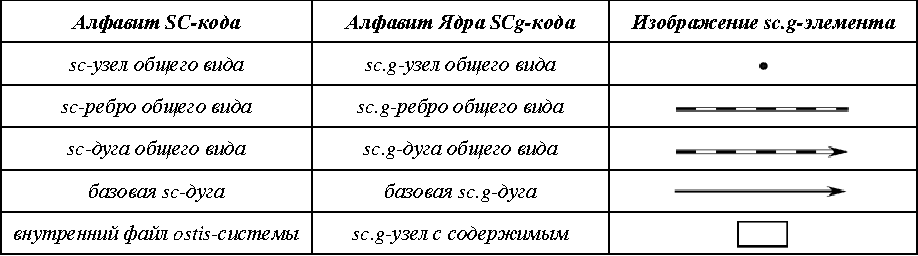
\includegraphics{figures/intro/scg/SCg-core-alphabet.pdf}}

%TODO сверить пропорции sc.g-элементов и изменить описание
\scnheader{sc.g-узел общего вида}
\scnidtf{\textit{sc.g-элемент}, являющийся графическим изображением \textit{sc-узла общего вида}}
\scnexplanation{Все \textit{sc-узлы}, не являющиеся знаками файлов, в тексте (конструкции) \textit{Ядра SCg-кода}, изображаются в виде небольших чёрных кругов одинакового диаметра, который обозначим через $\bm{d}$, и точная величина которого зависит от масштаба отображения \textit{sc.g-текста}.}

\scnheader{sc.g-ребро общего вида}
\scnidtf{\textit{sc.g-элемент}, являющийся графическим изображением \textit{sc-ребра общего вида}}
\scnexplanation{Каждое \textit{sc-ребро} в \textit{Ядре SCg-кода} изображается в виде широкой линии, в которой чередуются фрагменты со сплошной заливкой и без заливки, не имеющей самопересечений и имеющей общую толщину, равную примерно $\bm{0.7d}$.}

\scnheader{sc.g-дуга общего вида}
\scnidtf{\textit{sc.g-элемент}, являющийся графическим изображением \textit{sc-дуги общего вида}}
\scnexplanation{Каждая \textit{sc-дуга} в \textit{Ядре SCg-кода} изображается в виде широкой линии, в которой чередуются фрагменты со сплошной заливкой и без заливки, не имеющей самопересечений, имеющей общую толщину, равную примерно $\bm{0.7d}$ и имеющей изображение стрелочки на одном из концов этой линии.}

\scnheader{базовая sc.g-дуга}
\scnidtf{\textit{sc.g-элемент}, являющийся графическим изображением \textit{базовой sc-дуги}}
\scnexplanation{Каждая входящая в состав sc-текста \textit{базовая sc-дуга} в \textit{Ядре SCg-кода} изображается в виде линии произвольной формы, не имеющий самопересечений, имеющий толщину $\bm{0.4d}$, и имеющей изображение стрелочки на одном из ее концов.}

\scnheader{внутренний файл ostis-системы}
\scnidtf{sc-узел с содержимым}
\scnaddlevel{1}
\scniselement{часто используемый sc-идентификатор}
\scnaddlevel{-1}
\scnidtf{sc-узел, являющийся знаком внутреннего файла ostis-системы}
\scnidtf{sc-знак внутреннего файла ostis-системы}

\scnheader{sc.g-узел с содержимым}
\scnidtf{sc.g-узел, имеющий содержимое}
\scnidtf{sc.g-узел, являющийся знаком внутреннего файла ostis-системы}
\scnidtf{sc.g-знак внутреннего файла ostis-системы}
\scnidtf{sc.g-рамка, ограничивающая изображение (представление) внутреннего файла ostis-системы, обозначаемого этой sc.g-рамкой}
\scnidtf{sc.g-рамка}
\scnaddlevel{1}
\scnnote{\textit{sc.g-рамка} -- это всегда прямоугольник, максимальный размер которого не ограничивается, но минимальный фиксируется и соответствует \textit{sc.g-рамке}, внутри которой обозначаемый ею \textit{файл} не отображается.}
\scnaddlevel{-1}
\scnexplanation{Каждый входящий в sc-текст \textit{sc-узел, имеющий содержимое}, в \textit{Ядре SCg-кода} изображается в виде прямоугольника произвольного размера с толщиной линии $\bm{0.6d}$. Внутри этого прямоугольника отображается \textit{файл}, обозначаемый изображаемым \textit{sc-узлом}. Если нет необходимости изображать в тексте сам \textit{файл}, то \textit{sc-узел}, обозначающий такой \textit{файл}, в \textit{sc.g-тексте} изображается в виде прямоугольника со сторонами $\bm{2d}$ по вертикали и $\bm{4d}$ по горизонтали.}

\scnheader{Алфавит Ядра SCg-кода}
\scnnote{Трудно сразу поверить, что на основе такого простого алфавита можно построить удобный и \uline{универсальный} графовый язык. В рамках \textit{Документации Технологии OSTIS} мы постараемся Вас в этом убедить. Кроме того, нас не должна настораживать простота алфавита, поскольку человечество имеет большой опыт кодирования, хранения в памяти и передачи по каналам связи самых различных информационных ресурсов, используя алфавит, состоящий только из двух классов элементов -- единиц и нулей. 

Мы ведем речь о принципиально ином (графовом) способе кодирования информации в \textit{компьютерных системах}, но стараемся при этом свести это кодирование к достаточно простому алфавиту хотя бы для того, чтобы искусственно не усложнять проблему создания нового поколения компьютеров, основанных на указанном способе кодирования информации. 

Расширения \textit{Ядра SCg-кода} рассмотрим как направления перехода от текстов \textit{Ядра SCg-кода} к более компактным текстам. Но, поскольку это приводит к усложнению \textit{Синтаксиса SCg-кода} и, в первую очередь, к расширению \textit{Алфавита SCg-кода}, делать такие расширения необходимо обоснованно с учетом частоты встречаемости в рамках \textit{баз знаний ostis-систем} соответствующих фрагментов.}

\scnendstruct \scninlinesourcecommentpar{Завершили сегмент ``Описание Ядра SCg-кода''}

\scnsegmentheader{Описание Первого направления расширения Ядра SCg-кода}
\scnstartsubstruct

\bigskip
\scnheader{Первое направление расширения Ядра SCg-кода}

\scnexplanation{\textit{Первое направление синтаксического расширения Ядра SCg-кода} -- это \uline{приписывание} некоторым sc.g-элементам \textit{основных sc-идентификаторов*} (чаще всего - строковых идентификаторов, то есть имен) \textit{sc-элементов} , изображаемых этими \textit{sc.g-элементами}. Указываемые идентификаторы являются уникальным для каждого идентифицируемого (именуемого) \textit{sc.g-элемента}. Приписывание \textit{sc.g-элементам} уникальных идентификаторов дает возможность в рамках одного \textit{sc.g-текста} дублировать (копировать) некоторые \textit{sc.g-узлы} при условии, если \uline{всем} таким копиям будут приписаны соответствующие идентификаторы. Такое дублирование \textit{sc.g-узлов} является дополнительным средствам \uline{наглядного} размещения \textit{sc.g-текстов}. Кроме того, приписывание \textit{sc.g-элементу} соответствующего ему основного (уникального) \textit{sc-идентификатора*} представляет собой более компактный вариант изображения \textit{sc.g-текстов}.}

\scnheader{Пример sc.g-текста, трансформируемого по Первому направлению расширения Ядра SCg-кода}
\scneqscg{figures/intro/scg/scg_transf1.png}
\scniselement{sc.g-текст}
\scnexplanation{Здесь (в левом нижнем углу приведенного sc.g-текста) представлен \textit{sc.g-узел общего вида}, изображающий \textit{sc-узел общего вида}, которому соответствует \textit{основной sc-идентификатор*} в виде строки ``\textbf{\textit{ei}}''}
\scnrelfrom{трансформация sc.g-текста по Первому направлению расширения Ядра SCg-кода}{\scnfilescg{figures/intro/scg/scg_transf2.png}}
\scnaddlevel{1}
    \scniselement{sc.g-текст}
    \scnexplanation{\textit{sc.g-узлу общего вида} изображающему \textit{sc-узел}, внешним идентификатором которого является строка ``\textit{основной sc-идентификатор*}'' и который, соответственно является знаком \textit{бинарного ориентированного отношения}, каждая \textit{пара} которого связывает идентифицируемый \textit{sc-элемент} с его основным внешним sc-идентификатором, приписывается указанный внешний идентификатор изображаемого им \textit{sc-элемента}.}
    \scnrelfrom{трансформация sc.g-текста по Первому направлению расширения Ядра SCg-кода}{\scnfilescg{figures/intro/scg/scg_transf3.png}}
    \scnaddlevel{1}
        \scniselement{sc.g-текст} 
        \scnexplanation{В результате данной трансформации исходный \textit{sc.g-текст} трансформируется в один \textit{sc.g-общего вида}, которому приписывается \textit{основной sc-идентификатор} ``\textit{\textbf{ei}}''.}
    \scnaddlevel{-1}
\scnaddlevel{-1}


\scnheader{трансформация sc.g-текста по Первому направлению расширения Ядра SCg-кода*}
\scnidtf{Бинарное ориентированное отношение, каждая пара которого связывает исходный вид трансформируемого sc.g-текста и результат этой трансформации}
\scnnote{Подчеркнем, что рассматриваемая трансформация преобразует исходный текст Ядра \textit{SCg-кода} в текст, семантически эквивалентный, но принадлежащий не Ядру \textit{SCg-кода}, а его расширению.
}

\scnheader{синтаксическая трансформация*}
\scnidtf{синтаксическая трансформация информационной конструкции*}
\scnsuperset{синтаксическая трансформация sc.g-текста*}
\scnaddlevel{1}
\scnsuperset{трансформация sc.g-текста по Первому направлению расширения Ядра SCg-кода*}
\scnaddlevel{-1}

\scnendstruct \scninlinesourcecommentpar{Завершили сегмент "Описание первого направления расширения Ядра SCg-кода}
\bigskip

\scnsegmentheader{Описание Второго направления расширения Ядра SCg-кода}
\scnstartsubstruct

\scnheader{Второе направление расширения Ядра SCg-кода}
\scnexplanation{\textit{Второе направление расширения Ядра SCg-кода} -- это уточнение типологии \textit{константных постоянных сущностей} и расширение \textit{Алфавита Ядра SCg-кода}, позволяющее типологию \textit{константных постоянных сущностей} привести в соответствие с синтаксической типологией новых вводимых элементов \textit{Алфавита SCg-кода}. Рассмотрим подробнее sc.g-элементы, знаки \textit{константных постоянных сущностей} различного вида. Графическим признаком \textit{константных постоянных sc-узлов} в конструкциях SCg-кода является их изображение в виде \uline{окружностей} диаметра $3d$, где $d$ -- диаметр sc.g-узла общего вида. Такое изображение является более компактной записью факта принадлежности заданного sc-узла (назовем его $\bm{vi}$) классу sc-констант и классу обозначений постоянных сущностей. Запись этого факта в \textit{Ядре SCg-кода} потребует (1) явного изображения sc-узла, обозначающего класс всевозможных константных sc-элементов (класс \textit{sc-констант}), (2) явного изображения базовой sc-дуги, соединяющего изображение sc-узла, обозначающего класс sc-констант, с изображением заданного константного sc-узла, (3) явного изображение sc-узла, обозначающего класс всевозможных sc-элементов, обозначающих \textit{постоянные сущности}, (4) явного изображения базовой sc-дуги, соединяющего изображение sc-узла, обозначающего класс обозначений \textit{постоянных сущностей} с изображением рассматриваемого sc-узла $\bm{vi}$ (Смотрите \textit{Файл. Изображение спецификации sc.g-элемента средствами Ядра SCg-кода и Первого расширения Ядра SCg-кода}).

Общепринятая запись данного факта выглядит следующим образом:

``\textit{sc-константа} $\ni \bm{vi}$; \textit{постоянная сущность} $\ni \bm{v_i};$''

\textit{Константные постоянные sc-ребра} в конструкциях SCg-кода изображаются в виде двойной линии, каждая из которых имеет толщину примерно $d/7$, а расстояние между ними равно примерно $3d/7$. 

\textit{Константные постоянные sc-дуги} изображаются в виде такой же двойной линии, но со стрелочкой. Все \textit{базовые sc-дуги}, а также все sc-узлы, имеющие содержимое, по определению являются \textit{константными постоянными sc-элементами}. 

\textit{Константные sc.g-узлы}, изображаемые окружностями диаметра $3d$ и толщиной границы $d/5$, обозначают \textit{константные постоянные сущности}, о которых мало что известно, но известно то, что они не являются парами (то есть множествами, \textit{мощность*} которых равна 2) и, следовательно, не могут быть изображёны в виде sc.g-дуг или sc.g-рёбер. Но, если при этом об обозначаемой \textit{константной постоянной сущности} ($\bm{vi}$) известно, что она является классом сущностей, то явное указание принадлежности sc-элемента \textit{vi} всевозможных классов можно заменить на специальное графическое изображение sc-элемента \textit{vi}, предполагаемое указанную принадлежность. Это приводит к расширению  \textit{Алфавита SCg-кода} (см. \textit{Примеры sc.g-текстов, трансформируемых по Второму направлению расширения Ядра SCg-код}).

Аналогичным образом (см. \textit{Примеры sc.g-текстов, трансформируемых по Второму направлению расширения Ядра SCg-код}) вводятся: 
\begin{scnitemize}
\item sc.g-узел, являющийся изображением \textit{класса};  
\item sc.g-узел, являющийся изображением \textit{класса классов};  
\item sc.g-узел, являющийся изображением \textit{отношения}; 
\item sc.g-узел, являющийся изображением \textit{ролевого отношения}; 
\item sc.g-узел, являющийся изображением \textit{sc-структуры};  
\item sc.g-узел, являющийся изображением \textit{небинарной sc-связки};
\item sc.g-узел, являющийся изображением \textit{первичной сущности} (терминальной сущности, которая не является множеством, а также файлом, хранимым в памяти ostis-системы).
\end{scnitemize}

Важное место среди константных постоянных сущностей занимают \textit{константные постоянные пары принадлежности}, обозначаемое соответствующими \textit{sc.g-дугами}. Такие пары принадлежности и обозначающие их sc.g-дуги бывают позитивными, негативными и нечеткими. Константная постоянная позитивная sc.g-дуга принадлежности есть ничто иное, как \textit{базовая sc.g-дуга}. Константная постоянная негативная sc.g-дуга принадлежности изображается в виде \textit{базовой sc.g-дуги}, перечеркнутой штриховыми черточками. Константная постоянная нечёткая sc.g-дуга принадлежности изображается в виде "недочеркнутой"{} \textit{базовой sc.g-дуги}, с каждой стороны которой отображаются штрихи, по длине равные половине от длины штрихов, которыми перечеркнута \textit{константная постоянная негативная sc.g-дуга}.}

\scnheader{Файл. Изображение спецификации sc.g-элемента средствами Ядра SCg-кода и Второго направления расширения Ядра SCg-кода}
\scneqscg{figures/intro/scg/scg2ex.png}

\scnheader{Примеры sc.g-текстов, трансформируемых по Второму направлению расширения Ядра SCg-кода}
\scnstructinclusion

\scnmakeset{\scgfileitem{figures/intro/scg/scg2_ex1.png}\\
\scnaddlevel{1}
    \scnrelfrom{синтаксическая трансформация}{\scnfilescg{figures/intro/scg/scg2_ex1_1.png}}
    \scnaddlevel{1}
        \scnexplanation{Здесь вводится новый синтаксический вид \textit{sc.g-элементов} -- \textit{константный постоянный sc.g-узел общего вида}, изображаемый окружностью диаметра $3d$ и толщиной границы $d/5$.}
    \scnaddlevel{-1}
\scnaddlevel{-1};
\scgfileitem{figures/intro/scg/nodes/const_perm/sc.g_const_perm_class1.png}\\
\scnaddlevel{1}
    \scnrelfrom{синтаксическая трансформация}{\scnfilescg{figures/intro/scg/nodes/const_perm/sc.g_const_perm_class2.png}}
    \scnaddlevel{1}
        \scnexplanation{Здесь вводится новый синтаксический вид \textit{sc.g-элементов} -- \textit{константный постоянный sc.g-узел, обозначающий класс}, изображаемый как \textit{константный постоянный sc.g-узел} с "решеткой"{} внутри.}
    \scnaddlevel{-1}
\scnaddlevel{-1};
\scgfileitem{figures/intro/scg/nodes/const_perm/sc.g_const_perm_class_of_classes1.png}\\
\scnaddlevel{1}
    \scnrelfrom{синтаксическая трансформация}{\scnfilescg{figures/intro/scg/nodes/const_perm/sc.g_const_perm_class_of_classes2.png}}
    \scnaddlevel{1}
        \scnexplanation{Здесь вводится новый синтаксический вид \textit{sc.g-элементов} -- \textit{константный постоянный sc.g-узел, обозначающий класс классов}, изображаемый как \textit{константный постоянный sc.g-узел} с направленным вверх углом внутри.}
    \scnaddlevel{-1}
\scnaddlevel{-1};
\scgfileitem{figures/intro/scg/nodes/const_perm/sc.g_const_perm_norole1.png}\\
\scnaddlevel{1}
    \scnrelfrom{синтаксическая трансформация}{\scnfilescg{figures/intro/scg/nodes/const_perm/sc.g_const_perm_norole2.png}}
    \scnaddlevel{1}
        \scnexplanation{Здесь вводится новый синтаксический вид \textit{sc.g-элементов} -- \textit{константный постоянный sc.g-узел, обозначающий неролевое отношение}, изображаемый как \textit{константный постоянный sc.g-узел} с "крестиком"{} внутри.}
    \scnaddlevel{-1}
\scnaddlevel{-1};
\scgfileitem{figures/intro/scg/nodes/const_perm/sc.g_const_perm_role1.png}\\
\scnaddlevel{1}
    \scnrelfrom{синтаксическая трансформация}{\scnfilescg{figures/intro/scg/nodes/const_perm/sc.g_const_perm_role2.png}}
    \scnaddlevel{1}
        \scnexplanation{Здесь вводится новый синтаксический вид \textit{sc.g-элементов} -- \textit{константный постоянный sc.g-узел, обозначающий ролевое отношение}, изображаемый как \textit{константный постоянный sc.g-узел} с "плюсом"{} внутри.}
    \scnaddlevel{-1}
\scnaddlevel{-1};
\scgfileitem{figures/intro/scg/nodes/const_perm/sc.g_const_perm_structure1.png}\\
\scnaddlevel{1}
    \scnrelfrom{синтаксическая трансформация}{\scnfilescg{figures/intro/scg/nodes/const_perm/sc.g_const_perm_structure2.png}}
    \scnaddlevel{1}
        \scnexplanation{Здесь вводится новый синтаксический вид \textit{sc.g-элементов} -- \textit{константный постоянный sc.g-узел, обозначающий sc-структуру}, изображаемый как \textit{константный постоянный sc.g-узел} с точкой внутри.}
    \scnaddlevel{-1}
\scnaddlevel{-1};
\scgfileitem{figures/intro/scg/nodes/const_perm/sc.g_const_perm_primary_entity1.png}\\
\scnaddlevel{1}
    \scnrelfrom{синтаксическая трансформация}{\scnfilescg{figures/intro/scg/nodes/const_perm/sc.g_const_perm_primary_entity2.png}}
    \scnaddlevel{1}
        \scnexplanation{Здесь вводится новый синтаксический вид \textit{sc.g-элементов} -- \textit{константный постоянный sc.g-узел, обозначающий первичную сущность}, изображаемый как \textit{константный постоянный sc.g-узел} с  косой штриховкой внутри.}
    \scnaddlevel{-1}
\scnaddlevel{-1};
\scgfileitem{figures/intro/scg/nodes/const_perm/sc.g_const_perm_tuple1.png}\\
\scnaddlevel{1}
    \scnrelfrom{синтаксическая трансформация}{\scnfilescg{figures/intro/scg/nodes/const_perm/sc.g_const_perm_tuple2.png}}
    \scnaddlevel{1}
        \scnexplanation{Здесь вводится новый синтаксический вид \textit{sc.g-элементов} -- \textit{константный постоянный sc.g-узел, обозначающий небинарную sc-связку}, изображаемый как \textit{константный постоянный sc.g-узел} с горизонтальной линией внутри.}
    \scnaddlevel{-1}
\scnaddlevel{-1};
\scgfileitem{figures/intro/scg/arcs/const/scg_const_perm_noorien1.png}\\
\scnaddlevel{1}
    \scnrelfrom{синтаксическая трансформация}{\scnfilescg{figures/intro/scg/arcs/const/scg_const_perm_noorien2.png}}
    \scnaddlevel{1}
        \scnexplanation{Здесь вводится новый синтаксический вид \textit{sc.g-элементов} -- \textit{константное постоянное sc.g-ребро}, изображаемое двумя непрерывными параллельными линиями.}
    \scnaddlevel{-1}
\scnaddlevel{-1};
\scgfileitem{figures/intro/scg/arcs/const/scg_const_perm_orient1.png}\\
\scnaddlevel{1}
    \scnrelfrom{синтаксическая трансформация}{\scnfilescg{figures/intro/scg/arcs/const/scg_const_perm_orient2.png}}
    \scnaddlevel{1}
        \scnexplanation{Здесь вводится новый синтаксический вид \textit{sc.g-элементов} -- \textit{константная постоянная sc.g-дуга}, изображаемая двумя непрерывными параллельными линиями с общей стрелкой на одном из концов.}
    \scnaddlevel{-1}
\scnaddlevel{-1};
\scgfileitem{figures/intro/scg/arcs/const/scg_const_perm_positive1.png}\\
\scnaddlevel{1}
    \scnrelfrom{синтаксическая трансформация}{\scnfilescg{figures/intro/scg/arcs/const/scg_const_perm_positive2.png}}
    \scnaddlevel{1}
        \scnexplanation{\textit{Константная постоянная позитивная sc.g-дуга принадлежности} есть ничто иное, как \textit{базовая sc.g-дуга}.}
    \scnaddlevel{-1}
\scnaddlevel{-1};
\scgfileitem{figures/intro/scg/arcs/const/scg_const_perm_negative1.png}\\
\scnaddlevel{1}
    \scnrelfrom{синтаксическая трансформация}{\scnfilescg{figures/intro/scg/arcs/const/scg_const_perm_negative2.png}}
    \scnaddlevel{1}
        \scnexplanation{Здесь вводится новый синтаксический вид \textit{sc.g-элементов} -- \textit{константная постоянная негативная sc.g-дуга принадлежности}, изображается в виде \textit{базовой sc.g-дуги}, перечеркнутой штриховыми черточками.}
    \scnaddlevel{-1}
\scnaddlevel{-1};
\scgfileitem{figures/intro/scg/arcs/const/scg_const_perm_fuzzy1.png}\\
\scnaddlevel{1}
    \scnrelfrom{синтаксическая трансформация}{\scnfilescg{figures/intro/scg/arcs/const/scg_const_perm_fuzzy2.png}}
    \scnaddlevel{1}
        \scnexplanation{Здесь вводится новый синтаксический вид \textit{sc.g-элементов} -- \textit{константная постоянная нечеткая sc.g-дуга принадлежности}, которая изображается в виде "недочеркнутой"{} \textit{базовой sc.g-дуги}, с каждой стороны которой отображаются штрихи, по длине равные половине от длины штрихов, которыми перечеркнута \textit{константная постоянная негативная sc.g-дуга}.}
    \scnaddlevel{-1}
\scnaddlevel{-1}
}

\scnheader{Примеры sc.g-текста, записанного средствами Второго направления расширения Ядра SCg-кода}
\scnstructinclusion

\scnmakeset{\scgfileitem{figures/intro/scg/examples/scg_example_triangle.png}
\scnaddlevel{1}
\scniselementrole{пример}{sc.g-текст}
\scnexplanation{Данный sc.g-текст содержит следующую информацию:
\begin{scnitemize}
\item Сущности \textit{Треугольник ABC}~~ и ~~\textit{Треугольник CDE} являются треугольниками (принадлежат классу \textit{треугольников}). При этом известно, что площадь \textit{Треугольника CDE} в 4 раза больше, чем площадь \textit{Треугольника ABC}, но конкретные значения ллощадей не известны\char59
\item Сущность \textit{Отрезок DE} является отрезком (принадлежит классу \textit{отрезков}) и является стороной \textit{Треугольника CDE}. Кроме того, у \textit{Отрезка DE} есть длина, измерение которой в сантиметрах составляет 5. Обратите внимание, что в данном случае для упрощения понимания использовано бинарное отношение \textit{длина*}, которое является \textit{неосновным понятием} и в базе знаний заменяется на \textit{базовую sc-дугу}, связывающую величину как класс эквивалентности с конкретной сущностью, входящей в данный класс, в данном случае -- \textit{Отрезок DE}\char59  
\item Сущность \textit{Треугольник AEB} является треугольником и имеет \textit{внутренний угол*}~~~ \textit{Угол AEB}. В свою очередь, \textit{Угол AEB} является \textit{углом} и имеет \textit{косинус*}, равный 0,5\char59
\item \textit{Треугольник AEB} имеет \textit{сторону*} (не указывается, какая именно из сторон имеется в виду), \textit{средней точкой*} которой является \textit{Точка O}. В свою очередь, \textit{Точка O} является центром некоторой \textit{Окружности O}, которая относится к классу \textit{окружностей}.
\end{scnitemize}
}\scnaddlevel{-1};
\scgfileitem{figures/intro/scg/examples/scg_example_alice.png}
\scnaddlevel{1}
	\scnnote{Данный sc.g-текст основан на популярном примере, наглядно иллюстрируещем понятие семантической сети, известном как ``Социальная сеть Алисы''. Как видно из примера, данный текст описывает различные взаимосвязи персоны по имени Алиса, при этом некоторые из используемых отношений является ориентированными (например, ``работник*''), а некоторые -- неориентированными (например, ``друг*'').}
\scnaddlevel{-1}
}

\scnendstruct

\scnsegmentheader{Описание Третьего направления расширения Ядра SCg-кода}

\scnstartsubstruct

\bigskip
\scnfilelong{\textit{Третье направление расширения Ядра SCg-кода} -- это расширение его алфавита путем введения дополнительных sc.g-элементов, обозначающих \textit{константные временные сущности} различного вида. Признаком sc.g-элементов, обозначающих \textit{константные временные сущности} являются точечные линии (линии, состоящие из точек, размер которых равен размеру изображаемой линии и которые близко расположены друг к другу на расстоянии, равном половине их размера), с помощью которых рисуются окружности при изображении sc-узлов, а также линии при изображении sc-коннекторов.

Результатом \textit{Третьего направления расширения Ядра SCg-кода} является введение следующих видов sc.g-элементов (см. \textit{Примеры sc.g-текстов, трансформируемых по Третьему направлению расширения Ядра SCg-кода}).}

\scnheader{Примеры sc.g-текстов, трансформируемых по Третьему направлению расширения Ядра SCg-кода}
\scnstructinclusion
\scnmakeset{\scgfileitem{figures/intro/scg/nodes/const_temp/sc.g_const_temp_general_view1.png}\\
\scnaddlevel{1}
    \scnrelfrom{синтаксическая трансформация}{\scnfilescg{figures/intro/scg/nodes/const_temp/sc.g_const_temp_general_view2.png}}
    \scnaddlevel{1}
        \scnexplanation{Здесь вводится новый синтаксический вид \textit{sc.g-элементов} -- \textit{константный временный sc.g-узел общего вида}, изображаемый точечной окружностью диаметра $3d$ и толщиной границы $d/5$.}
    \scnaddlevel{-1}
\scnaddlevel{-1};
\scgfileitem{figures/intro/scg/nodes/const_temp/sc.g_const_temp_class1.png}\\
\scnaddlevel{1}
    \scnrelfrom{синтаксическая трансформация}{\scnfilescg{figures/intro/scg/nodes/const_temp/sc.g_const_temp_class2.png}}
    \scnaddlevel{1}
        \scnexplanation{Здесь вводится новый синтаксический вид \textit{sc.g-элементов} -- \textit{константный временный sc.g-узел, обозначающий класс}, изображаемый как \textit{константный временный sc.g-узел} с "решеткой"{} внутри.}
    \scnaddlevel{-1}
\scnaddlevel{-1};
\scgfileitem{figures/intro/scg/nodes/const_temp/sc.g_const_temp_class_of_classes1.png}\\
\scnaddlevel{1}
    \scnrelfrom{синтаксическая трансформация}{\scnfilescg{figures/intro/scg/nodes/const_temp/sc.g_const_temp_class_of_classes2.png}}
    \scnaddlevel{1}
        \scnexplanation{Здесь вводится новый синтаксический вид \textit{sc.g-элементов} -- \textit{константный временный sc.g-узел, обозначающий класс классов}, изображаемый как \textit{константный временный sc.g-узел} с направленным вверх углом внутри.}
    \scnaddlevel{-1}
\scnaddlevel{-1};
\scgfileitem{figures/intro/scg/nodes/const_temp/sc.g_const_temp_norole1.png}\\
\scnaddlevel{1}
    \scnrelfrom{синтаксическая трансформация}{\scnfilescg{figures/intro/scg/nodes/const_temp/sc.g_const_temp_norole2.png}}
    \scnaddlevel{1}
        \scnexplanation{Здесь вводится новый синтаксический вид \textit{sc.g-элементов} -- \textit{константный временный sc.g-узел, обозначающий неролевое отношение}, изображаемый как \textit{константный временный sc.g-узел} с "крестиком"{} внутри.}
    \scnaddlevel{-1}
\scnaddlevel{-1};
\scgfileitem{figures/intro/scg/nodes/const_temp/sc.g_const_temp_role1.png}\\
\scnaddlevel{1}
    \scnrelfrom{синтаксическая трансформация}{\scnfilescg{figures/intro/scg/nodes/const_temp/sc.g_const_temp_role2.png}}
    \scnaddlevel{1}
        \scnexplanation{Здесь вводится новый синтаксический вид \textit{sc.g-элементов} -- \textit{константный временный sc.g-узел, обозначающий ролевое отношение}, изображаемый как \textit{константный временный sc.g-узел} с "плюсом"{} внутри.}
    \scnaddlevel{-1}
\scnaddlevel{-1};
\scgfileitem{figures/intro/scg/nodes/const_temp/sc.g_const_temp_structure1.png}\\
\scnaddlevel{1}
    \scnrelfrom{синтаксическая трансформация}{\scnfilescg{figures/intro/scg/nodes/const_temp/sc.g_const_temp_structure2.png}}
    \scnaddlevel{1}
        \scnexplanation{Здесь вводится новый синтаксический вид \textit{sc.g-элементов} -- \textit{константный временный sc.g-узел, обозначающий sc-структуру}, изображаемый как \textit{константный временный sc.g-узел} с точкой внутри.}
    \scnaddlevel{-1}
\scnaddlevel{-1};
\scgfileitem{figures/intro/scg/nodes/const_temp/sc.g_const_temp_primary_entity1.png}\\
\scnaddlevel{1}
    \scnrelfrom{синтаксическая трансформация}{\scnfilescg{figures/intro/scg/nodes/const_temp/sc.g_const_temp_primary_entity2.png}}
    \scnaddlevel{1}
        \scnexplanation{Здесь вводится новый синтаксический вид \textit{sc.g-элементов} -- \textit{константный временный sc.g-узел, обозначающий первичную сущность}, изображаемый как \textit{константный временный sc.g-узел} с  косой штриховкой внутри.}
    \scnaddlevel{-1}
\scnaddlevel{-1};
\scgfileitem{figures/intro/scg/nodes/const_temp/sc.g_const_temp_tuple1.png}\\
\scnaddlevel{1}
    \scnrelfrom{синтаксическая трансформация}{\scnfilescg{figures/intro/scg/nodes/const_temp/sc.g_const_temp_tuple2.png}}
    \scnaddlevel{1}
        \scnexplanation{Здесь вводится новый синтаксический вид \textit{sc.g-элементов} -- \textit{константный временный sc.g-узел, обозначающий небинарную sc-связку}, изображаемый как \textit{константный временный sc.g-узел} с горизонтальной линией внутри.}
    \scnaddlevel{-1}
\scnaddlevel{-1};
\scgfileitem{figures/intro/scg/arcs/const/scg_const_temp_noorien1.png}\\
\scnaddlevel{1}
    \scnrelfrom{синтаксическая трансформация}{\scnfilescg{figures/intro/scg/arcs/const/scg_const_temp_noorien2.png}}
    \scnaddlevel{1}
        \scnexplanation{Здесь вводится новый синтаксический вид \textit{sc.g-элементов} -- \textit{константное временное sc.g-ребро}, изображаемое двумя точечными параллельными линиями.}
    \scnaddlevel{-1}
\scnaddlevel{-1};
\scgfileitem{figures/intro/scg/arcs/const/scg_const_temp_orient1.png}\\
\scnaddlevel{1}
    \scnrelfrom{синтаксическая трансформация}{\scnfilescg{figures/intro/scg/arcs/const/scg_const_temp_orient2.png}}
    \scnaddlevel{1}
        \scnexplanation{Здесь вводится новый синтаксический вид \textit{sc.g-элементов} -- \textit{константная временная sc.g-дуга}, изображаемая двумя точечными параллельными линиями с общей стрелкой на одном из концов.}
    \scnaddlevel{-1}
\scnaddlevel{-1};
\scgfileitem{figures/intro/scg/arcs/const/scg_const_temp_positive1.png}\\
\scnaddlevel{1}
    \scnrelfrom{синтаксическая трансформация}{\scnfilescg{figures/intro/scg/arcs/const/scg_const_temp_positive2.png}}
    \scnaddlevel{1}
        \scnexplanation{Здесь вводится новый синтаксический вид \textit{sc.g-элементов} -- \textit{константная временная позитивная sc.g-дуга принадлежности}, изображаемая точечной линией со стрелкой на конце.}
    \scnaddlevel{-1}
\scnaddlevel{-1};
\scgfileitem{figures/intro/scg/arcs/const/scg_const_temp_negative1.png}\\
\scnaddlevel{1}
    \scnrelfrom{синтаксическая трансформация}{\scnfilescg{figures/intro/scg/arcs/const/scg_const_temp_negative2.png}}
    \scnaddlevel{1}
        \scnexplanation{Здесь вводится новый синтаксический вид \textit{sc.g-элементов} -- \textit{константная временная негативная sc.g-дуга принадлежности}, изображаемая точечной линией, перечеркнутой штриховыми черточками, со стрелкой на конце.}
    \scnaddlevel{-1}
\scnaddlevel{-1};
\scgfileitem{figures/intro/scg/arcs/const/scg_const_temp_fuzzy1.png}\\
\scnaddlevel{1}
    \scnrelfrom{синтаксическая трансформация}{\scnfilescg{figures/intro/scg/arcs/const/scg_const_temp_fuzzy2.png}}
    \scnaddlevel{1}
        \scnexplanation{Здесь вводится новый синтаксический вид \textit{sc.g-элементов} -- \textit{константная временная нечеткая sc.g-дуга принадлежности}, которая изображается в виде "недочеркнутой"{} \textit{\textit{константной временной позитивная sc.g-дуги принадлежности}, с каждой стороны которой отображаются штрихи, по длине равные половине от длины штрихов, которыми перечеркнута \textit{константная постоянная негативная sc.g-дуга}.}
    \scnaddlevel{-1}
\scnaddlevel{-1}
}
}

\scnendstruct

\scnsegmentheader{Описание Четвёртого направления расширения Ядра SCg-кода}

\scnstartsubstruct

\bigskip
\scnfilelong{Четвёртое направление расширения \textit{Ядра SCg-кода} -- это расширение его алфавита путем введения дополнительных элементов, обозначающих \textit{переменные постоянные сущности} различного вида. Признаком sc.g-элементов, обозначающих сущности указанного класса, являются квадратики для изображения обозначений \textit{переменных постоянных сущностей}, не являющихся бинарными связями, а также пунктирные и штрих-пунктирные линии для изображения \textit{переменных постоянных бинарных связей}. 

Подчеркнем, что \textit{переменные постоянные сущности} могут отличаться друг от друга по характеру их \textit{области значений*}. Этими значениями в общем случае могут быть как \textit{константные постоянные сущности}, так и \textit{переменные постоянные сущности}. В любом случае, значение \textit{переменной сущности} является либо \textit{константной сущностью}, либо \textit{переменной сущностью}. Если каждое значение переменной является константой, то такую переменную будем называть \textit{переменной первого уровня}. Если каждое значение переменной является \textit{переменной первого уровня}, то такую переменную будем называть \textit{переменной второго уровня}. 

\textit{Переменная постоянная сущность первого уровня } (первичная sc-переменная), не являющаяся бинарной связью -- это переменная, каждым значением которой является \textit{константная постоянная сущность}, не являющаяся бинарной связью. Такая переменная изображается квадратиком, который ориентирован по вертикали и горизонтали. 

\textit{переменная постоянная сущность второго уровня} (вторичная sc-переменная), не являющаяся бинарной связью, изображается квадратиком, повернутым на 45$^\circ$. 

Указанная выше семантика таких изображений приписывается \uline{по умолчанию}. Это означает, что, если обозначаемая sc-переменная имеет более сложную структуру области её значений (является sc-переменной третьего и выше уровня или sc-переменной, значения которой имеют различный логический уровень), то эта область должна быть специфицирована явно, при этом такая sc-переменная в SCg-коде изображается так же, как первичная sc-переменная.}

\scnheader{Примеры sc.g-текстов, трансформируемых по Четвертому направлению расширения Ядра SCg-кода}
\scnstructinclusion
\scnmakeset{\scgfileitem{figures/intro/scg/nodes/var_perm/sc.g_var_perm_general_view1.png}\\
\scnaddlevel{1}
    \scnrelfrom{синтаксическая трансформация}{\scnfilescg{figures/intro/scg/nodes/var_perm/sc.g_var_perm_general_view2.png}}
    \scnaddlevel{1}
        \scnexplanation{Здесь вводится новый синтаксический вид \textit{sc.g-элементов} -- \textit{переменный постоянный sc.g-узел общего вида}, изображаемый квадратиком cj со стороной длины $3d$ и толщиной границы $d/5$.}
    \scnaddlevel{-1}
\scnaddlevel{-1};
\scgfileitem{figures/intro/scg/nodes/var_perm/sc.g_var_perm_class1.png}\\
\scnaddlevel{1}
    \scnrelfrom{синтаксическая трансформация}{\scnfilescg{figures/intro/scg/nodes/var_perm/sc.g_var_perm_class2.png}}
    \scnaddlevel{1}
        \scnexplanation{Здесь вводится новый синтаксический вид \textit{sc.g-элементов} -- \textit{переменный постоянный sc.g-узел, обозначающий класс}, изображаемый как \textit{переменный постоянный sc.g-узел} с "решеткой"{} внутри.}
    \scnaddlevel{-1}
\scnaddlevel{-1};
\scgfileitem{figures/intro/scg/nodes/var_perm/sc.g_var_perm_class_of_classes1.png}\\
\scnaddlevel{1}
    \scnrelfrom{синтаксическая трансформация}{\scnfilescg{figures/intro/scg/nodes/var_perm/sc.g_var_perm_class_of_classes2.png}}
    \scnaddlevel{1}
        \scnexplanation{Здесь вводится новый синтаксический вид \textit{sc.g-элементов} -- \textit{переменный постоянный sc.g-узел, обозначающий класс классов}, изображаемый как \textit{переменный постоянный sc.g-узел} с направленным вверх углом внутри.}
    \scnaddlevel{-1}
\scnaddlevel{-1};
\scgfileitem{figures/intro/scg/nodes/var_perm/sc.g_var_perm_norole1.png}\\
\scnaddlevel{1}
    \scnrelfrom{синтаксическая трансформация}{\scnfilescg{figures/intro/scg/nodes/var_perm/sc.g_var_perm_norole2.png}}
    \scnaddlevel{1}
        \scnexplanation{Здесь вводится новый синтаксический вид \textit{sc.g-элементов} -- \textit{переменный постоянный sc.g-узел, обозначающий неролевое отношение}, изображаемый как \textit{переменный постоянный sc.g-узел} с "крестиком"{} внутри.}
    \scnaddlevel{-1}
\scnaddlevel{-1};
\scgfileitem{figures/intro/scg/nodes/var_perm/sc.g_var_perm_role1.png}\\
\scnaddlevel{1}
    \scnrelfrom{синтаксическая трансформация}{\scnfilescg{figures/intro/scg/nodes/var_perm/sc.g_var_perm_role2.png}}
    \scnaddlevel{1}
        \scnexplanation{Здесь вводится новый синтаксический вид \textit{sc.g-элементов} -- \textit{переменный постоянный sc.g-узел, обозначающий ролевое отношение}, изображаемый как \textit{переменный постоянный sc.g-узел} с "плюсом"{} внутри..}
    \scnaddlevel{-1}
\scnaddlevel{-1};
\scgfileitem{figures/intro/scg/nodes/var_perm/sc.g_var_perm_structure1.png}\\
\scnaddlevel{1}
    \scnrelfrom{синтаксическая трансформация}{\scnfilescg{figures/intro/scg/nodes/var_perm/sc.g_var_perm_structure2.png}}
    \scnaddlevel{1}
        \scnexplanation{Здесь вводится новый синтаксический вид \textit{sc.g-элементов} -- \textit{переменный постоянный sc.g-узел, обозначающий sc-структуру}, изображаемый как \textit{переменный постоянный sc.g-узел} с точкой внутри.}
    \scnaddlevel{-1}
\scnaddlevel{-1};
\scgfileitem{figures/intro/scg/nodes/var_perm/sc.g_var_perm_primary_entity1.png}\\
\scnaddlevel{1}
    \scnrelfrom{синтаксическая трансформация}{\scnfilescg{figures/intro/scg/nodes/var_perm/sc.g_var_perm_primary_entity2.png}}
    \scnaddlevel{1}
        \scnexplanation{Здесь вводится новый синтаксический вид \textit{sc.g-элементов} -- \textit{переменный постоянный sc.g-узел, обозначающий первичную сущность}, изображаемый как \textit{переменный постоянный sc.g-узел} с  косой штриховкой внутри.}
    \scnaddlevel{-1}
\scnaddlevel{-1};
\scgfileitem{figures/intro/scg/nodes/var_perm/sc.g_var_perm_tuple1.png}\\
\scnaddlevel{1}
    \scnrelfrom{синтаксическая трансформация}{\scnfilescg{figures/intro/scg/nodes/var_perm/sc.g_var_perm_tuple2.png}}
    \scnaddlevel{1}
        \scnexplanation{Здесь вводится новый синтаксический вид \textit{sc.g-элементов} -- \textit{переменный постоянный sc.g-узел, обозначающий небинарную sc-связку}, изображаемый как \textit{переменный постоянный sc.g-узел} с горизонтальной линией внутри.}
    \scnaddlevel{-1}
\scnaddlevel{-1};
\scgfileitem{figures/intro/scg/arcs/var/scg_var_perm_noorien1.png}\\
\scnaddlevel{1}
    \scnrelfrom{синтаксическая трансформация}{\scnfilescg{figures/intro/scg/arcs/var/scg_var_perm_noorien2.png}}
    \scnaddlevel{1}
        \scnexplanation{Здесь вводится новый синтаксический вид \textit{sc.g-элементов} -- \textit{переменное постоянное sc.g-ребро}, изображаемое двумя пунктирными параллельными линиями.}
    \scnaddlevel{-1}
\scnaddlevel{-1};
\scgfileitem{figures/intro/scg/arcs/var/scg_var_perm_orient1.png}\\
\scnaddlevel{1}
    \scnrelfrom{синтаксическая трансформация}{\scnfilescg{figures/intro/scg/arcs/var/scg_var_perm_orient2.png}}
    \scnaddlevel{1}
        \scnexplanation{Здесь вводится новый синтаксический вид \textit{sc.g-элементов} -- \textit{переменная постоянная sc.g-дуга}, изображаемая двумя пунктирными параллельными линиями с общей стрелкой на одном из концов.}
    \scnaddlevel{-1}
\scnaddlevel{-1};
\scgfileitem{figures/intro/scg/arcs/var/scg_var_perm_positive1.png}\\
\scnaddlevel{1}
    \scnrelfrom{синтаксическая трансформация}{\scnfilescg{figures/intro/scg/arcs/var/scg_var_perm_positive2.png}}
    \scnaddlevel{1}
        \scnexplanation{\textit{переменная постоянная позитивная sc.g-дуга принадлежности}, изображаемая пунктирной линией со стрелкой на конце.}
    \scnaddlevel{-1}
\scnaddlevel{-1};
\scgfileitem{figures/intro/scg/arcs/var/scg_var_perm_negative1.png}\\
\scnaddlevel{1}
    \scnrelfrom{синтаксическая трансформация}{\scnfilescg{figures/intro/scg/arcs/var/scg_var_perm_negative2.png}}
    \scnaddlevel{1}
        \scnexplanation{Здесь вводится новый синтаксический вид \textit{sc.g-элементов} -- \textit{переменная постоянная негативная sc.g-дуга принадлежности}, изображается в виде \textit{переменной постоянной позитивной sc.g-дуги принадлежности}, перечеркнутой штриховыми черточками.}
    \scnaddlevel{-1}
\scnaddlevel{-1};
\scgfileitem{figures/intro/scg/arcs/var/scg_var_perm_fuzzy1.png}\\
\scnaddlevel{1}
    \scnrelfrom{синтаксическая трансформация}{\scnfilescg{figures/intro/scg/arcs/var/scg_var_perm_fuzzy2.png}}
    \scnaddlevel{1}
        \scnexplanation{Здесь вводится новый синтаксический вид \textit{sc.g-элементов} -- \textit{переменная постоянная нечеткая sc.g-дуга принадлежности}, которая изображается в виде "недочеркнутой"{} \textit{переменной постоянной позитивной sc.g-дуги принадлежности}, с каждой стороны которой отображаются штрихи, по длине равные половине от длины штрихов, которыми перечеркнута \textit{переменная постоянная негативная sc.g-дуга}.}
    \scnaddlevel{-1}
\scnaddlevel{-1};
\scgfileitem{figures/intro/scg/nodes/metavar_perm/sc.g_metavar_perm_general_view1.png}\\
\scnaddlevel{1}
    \scnrelfrom{синтаксическая трансформация}{\scnfilescg{figures/intro/scg/nodes/metavar_perm/sc.g_metavar_perm_general_view2.png}}
    \scnaddlevel{1}
        \scnexplanation{Здесь вводится новый синтаксический вид \textit{sc.g-элементов} -- \textit{метапеременный постоянный sc.g-узел общего вида}, изображаемый квадратиком, повернутым на 45 градусов.}
    \scnaddlevel{-1}
\scnaddlevel{-1};
\scgfileitem{figures/intro/scg/nodes/metavar_perm/sc.g_metavar_perm_class1.png}\\
\scnaddlevel{1}
    \scnrelfrom{синтаксическая трансформация}{\scnfilescg{figures/intro/scg/nodes/metavar_perm/sc.g_metavar_perm_class2.png}}
    \scnaddlevel{1}
        \scnexplanation{Здесь вводится новый синтаксический вид \textit{sc.g-элементов} -- \textit{метапеременный постоянный sc.g-узел, обозначающий класс}, изображаемый как \textit{метапеременный постоянный sc.g-узел} с "решеткой"{} внутри.}
    \scnaddlevel{-1}
\scnaddlevel{-1};
\scgfileitem{figures/intro/scg/nodes/metavar_perm/sc.g_metavar_perm_class_of_classes1.png}\\
\scnaddlevel{1}
    \scnrelfrom{синтаксическая трансформация}{\scnfilescg{figures/intro/scg/nodes/metavar_perm/sc.g_metavar_perm_class_of_classes2.png}}
    \scnaddlevel{1}
        \scnexplanation{Здесь вводится новый синтаксический вид \textit{sc.g-элементов} -- \textit{метапеременный постоянный sc.g-узел, обозначающий класс классов}, изображаемый как \textit{метапеременный постоянный sc.g-узел} с направленным вверх углом внутри.}
    \scnaddlevel{-1}
\scnaddlevel{-1};
\scgfileitem{figures/intro/scg/nodes/metavar_perm/sc.g_metavar_perm_norole1.png}\\
\scnaddlevel{1}
    \scnrelfrom{синтаксическая трансформация}{\scnfilescg{figures/intro/scg/nodes/metavar_perm/sc.g_metavar_perm_norole2.png}}
    \scnaddlevel{1}
        \scnexplanation{Здесь вводится новый синтаксический вид \textit{sc.g-элементов} -- \textit{метапеременный постоянный sc.g-узел, обозначающий неролевое отношение}, изображаемый как \textit{метапеременный постоянный sc.g-узел} с "крестиком"{} внутри.}
    \scnaddlevel{-1}
\scnaddlevel{-1};
\scgfileitem{figures/intro/scg/nodes/metavar_perm/sc.g_metavar_perm_role1.png}\\
\scnaddlevel{1}
    \scnrelfrom{синтаксическая трансформация}{\scnfilescg{figures/intro/scg/nodes/metavar_perm/sc.g_metavar_perm_role2.png}}
    \scnaddlevel{1}
        \scnexplanation{Здесь вводится новый синтаксический вид \textit{sc.g-элементов} -- \textit{метапеременный постоянный sc.g-узел, обозначающий ролевое отношение}, изображаемый как \textit{метапеременный постоянный sc.g-узел} с "плюсом"{} внутри..}
    \scnaddlevel{-1}
\scnaddlevel{-1};
\scgfileitem{figures/intro/scg/nodes/metavar_perm/sc.g_metavar_perm_structure1.png}\\
\scnaddlevel{1}
    \scnrelfrom{синтаксическая трансформация}{\scnfilescg{figures/intro/scg/nodes/metavar_perm/sc.g_metavar_perm_structure2.png}}
    \scnaddlevel{1}
        \scnexplanation{Здесь вводится новый синтаксический вид \textit{sc.g-элементов} -- \textit{метапеременный постоянный sc.g-узел, обозначающий sc-структуру}, изображаемый как \textit{метапеременный постоянный sc.g-узел} с точкой внутри.}
    \scnaddlevel{-1}
\scnaddlevel{-1};
\scgfileitem{figures/intro/scg/nodes/metavar_perm/sc.g_metavar_perm_primary_entity1.png}\\
\scnaddlevel{1}
    \scnrelfrom{синтаксическая трансформация}{\scnfilescg{figures/intro/scg/nodes/metavar_perm/sc.g_metavar_perm_primary_entity2.png}}
    \scnaddlevel{1}
        \scnexplanation{Здесь вводится новый синтаксический вид \textit{sc.g-элементов} -- \textit{метапеременный постоянный sc.g-узел, обозначающий первичную сущность}, изображаемый как \textit{метапеременный постоянный sc.g-узел} с  косой штриховкой внутри.}
    \scnaddlevel{-1}
\scnaddlevel{-1};
\scgfileitem{figures/intro/scg/nodes/metavar_perm/sc.g_metavar_perm_tuple1.png}\\
\scnaddlevel{1}
    \scnrelfrom{синтаксическая трансформация}{\scnfilescg{figures/intro/scg/nodes/metavar_perm/sc.g_metavar_perm_tuple2.png}}
    \scnaddlevel{1}
        \scnexplanation{Здесь вводится новый синтаксический вид \textit{sc.g-элементов} -- \textit{метапеременный постоянный sc.g-узел, обозначающий небинарную sc-связку}, изображаемый как \textit{метапеременный постоянный sc.g-узел} с горизонтальной линией внутри.}
    \scnaddlevel{-1}
\scnaddlevel{-1};
\scgfileitem{figures/intro/scg/arcs/meta/scg_metavar_perm_noorien1.png}\\
\scnaddlevel{1}
    \scnrelfrom{синтаксическая трансформация}{\scnfilescg{figures/intro/scg/arcs/meta/scg_metavar_perm_noorien2.png}}
    \scnaddlevel{1}
        \scnexplanation{Здесь вводится новый синтаксический вид \textit{sc.g-элементов} -- \textit{метапеременное постоянное sc.g-ребро}, изображаемое двумя штрих-пунктирными параллельными линиями.}
    \scnaddlevel{-1}
\scnaddlevel{-1};
\scgfileitem{figures/intro/scg/arcs/meta/scg_metavar_perm_orient1.png}\\
\scnaddlevel{1}
    \scnrelfrom{синтаксическая трансформация}{\scnfilescg{figures/intro/scg/arcs/meta/scg_metavar_perm_orient2.png}}
    \scnaddlevel{1}
        \scnexplanation{Здесь вводится новый синтаксический вид \textit{sc.g-элементов} -- \textit{метапеременная постоянная sc.g-дуга}, изображаемая двумя штрих-пунктирными непрерывными параллельными линиями с общей стрелкой на одном из концов.}
    \scnaddlevel{-1}
\scnaddlevel{-1};
\scgfileitem{figures/intro/scg/arcs/meta/scg_metavar_perm_positive1.png}\\
\scnaddlevel{1}
    \scnrelfrom{синтаксическая трансформация}{\scnfilescg{figures/intro/scg/arcs/meta/scg_metavar_perm_positive2.png}}
    \scnaddlevel{1}
        \scnexplanation{\textit{метапеременная постоянная позитивная sc.g-дуга принадлежности}, изображаемая штрих-пунктирной линией со стрелкой на конце.}
    \scnaddlevel{-1}
\scnaddlevel{-1};
\scgfileitem{figures/intro/scg/arcs/meta/scg_metavar_perm_negative1.png}\\
\scnaddlevel{1}
    \scnrelfrom{синтаксическая трансформация}{\scnfilescg{figures/intro/scg/arcs/meta/scg_metavar_perm_negative2.png}}
    \scnaddlevel{1}
        \scnexplanation{Здесь вводится новый синтаксический вид \textit{sc.g-элементов} -- \textit{метапеременная постоянная негативная sc.g-дуга принадлежности}, изображается в виде \textit{метапеременной постоянной позитивной sc.g-дуги принадлежности}, перечеркнутой штриховыми черточками.}
    \scnaddlevel{-1}
\scnaddlevel{-1};
\scgfileitem{figures/intro/scg/arcs/meta/scg_metavar_perm_fuzzy1.png}\\
\scnaddlevel{1}
    \scnrelfrom{синтаксическая трансформация}{\scnfilescg{figures/intro/scg/arcs/meta/scg_metavar_perm_fuzzy2.png}}
    \scnaddlevel{1}
        \scnexplanation{Здесь вводится новый синтаксический вид \textit{sc.g-элементов} -- \textit{метапеременная постоянная нечеткая sc.g-дуга принадлежности}, которая изображается в виде "недочеркнутой"{} \textit{метапеременной постоянной позитивной sc.g-дуги принадлежности}, с каждой стороны которой отображаются штрихи, по длине равные половине от длины штрихов, которыми перечеркнута \textit{метапеременная постоянная негативная sc.g-дуга}.}
    \scnaddlevel{-1}
\scnaddlevel{-1}
}

\scnendstruct

\scnsegmentheader{Описание Пятого направления расширения Ядра SCg-кода}

\scnstartsubstruct

\bigskip
\scnfilelong{\textit{Пятое направление расширения Ядра SCg-кода} -- это расширение его алфавита путем введения дополнительных \textit{sc.g-элементов}, обозначающих \textit{переменные временные сущности} различного вида. Указанные дополнительные \textit{sc.g-элементы} аналогичны тем, которые введены в рамках \textit{Четвертого направления расширения Ядра SCg-кода}, и отличаются только тем, что в \textit{Пятом направлении расширении Ядра SCg-кода} речь идёт о переменных \uline{временных} сущностях, а в \textit{Четвертом направлении расширения Ядра SCg-кода} -- о переменных \uline{постоянных} сущностях.}

\scnheader{Примеры sc.g-текстов, трансформируемых по Пятому направлению расширения Ядра SCg-кода}
\scnstructinclusion

\scnmakeset{\scgfileitem{figures/intro/scg/nodes/var_temp/sc.g_var_temp_general_view1.png}\\
\scnaddlevel{1}
    \scnrelfrom{синтаксическая трансформация}{\scnfilescg{figures/intro/scg/nodes/var_temp/sc.g_var_temp_general_view2.png}}
    \scnaddlevel{1}
        \scnexplanation{Здесь вводится новый синтаксический вид \textit{sc.g-элементов} -- \textit{переменный временный sc.g-узел общего вида}, изображаемый точечным квадратиком диаметра $3d$ и толщиной границы $d/5$.}
    \scnaddlevel{-1}
\scnaddlevel{-1};
\scgfileitem{figures/intro/scg/nodes/var_temp/sc.g_var_temp_class1.png}\\
\scnaddlevel{1}
    \scnrelfrom{синтаксическая трансформация}{\scnfilescg{figures/intro/scg/nodes/var_temp/sc.g_var_temp_class2.png}}
    \scnaddlevel{1}
        \scnexplanation{Здесь вводится новый синтаксический вид \textit{sc.g-элементов} -- \textit{переменный временный sc.g-узел, обозначающий класс}, изображаемый как \textit{переменный временный sc.g-узел} с "решеткой"{} внутри.}
    \scnaddlevel{-1}
\scnaddlevel{-1};
\scgfileitem{figures/intro/scg/nodes/var_temp/sc.g_var_temp_class_of_classes1.png}\\
\scnaddlevel{1}
    \scnrelfrom{синтаксическая трансформация}{\scnfilescg{figures/intro/scg/nodes/var_temp/sc.g_var_temp_class_of_classes2.png}}
    \scnaddlevel{1}
        \scnexplanation{Здесь вводится новый синтаксический вид \textit{sc.g-элементов} -- \textit{переменный временный sc.g-узел, обозначающий класс классов}, изображаемый как \textit{переменный временный sc.g-узел} с направленным вверх углом внутри.}
    \scnaddlevel{-1}
\scnaddlevel{-1};
\scgfileitem{figures/intro/scg/nodes/var_temp/sc.g_var_temp_norole1.png}\\
\scnaddlevel{1}
    \scnrelfrom{синтаксическая трансформация}{\scnfilescg{figures/intro/scg/nodes/var_temp/sc.g_var_temp_norole2.png}}
    \scnaddlevel{1}
        \scnexplanation{Здесь вводится новый синтаксический вид \textit{sc.g-элементов} -- \textit{переменный временный sc.g-узел, обозначающий неролевое отношение}, изображаемый как \textit{переменный временный sc.g-узел} с "крестиком"{} внутри.}
    \scnaddlevel{-1}
\scnaddlevel{-1};
\scgfileitem{figures/intro/scg/nodes/var_temp/sc.g_var_temp_role1.png}\\
\scnaddlevel{1}
    \scnrelfrom{синтаксическая трансформация}{\scnfilescg{figures/intro/scg/nodes/var_temp/sc.g_var_temp_role2.png}}
    \scnaddlevel{1}
        \scnexplanation{Здесь вводится новый синтаксический вид \textit{sc.g-элементов} -- \textit{переменный временный sc.g-узел, обозначающий ролевое отношение}, изображаемый как \textit{переменный временный sc.g-узел} с "плюсом"{} внутри..}
    \scnaddlevel{-1}
\scnaddlevel{-1};
\scgfileitem{figures/intro/scg/nodes/var_temp/sc.g_var_temp_structure1.png}\\
\scnaddlevel{1}
    \scnrelfrom{синтаксическая трансформация}{\scnfilescg{figures/intro/scg/nodes/var_temp/sc.g_var_temp_structure2.png}}
    \scnaddlevel{1}
        \scnexplanation{Здесь вводится новый синтаксический вид \textit{sc.g-элементов} -- \textit{переменный временный sc.g-узел, обозначающий sc-структуру}, изображаемый как \textit{переменный временный sc.g-узел} с точкой внутри.}
    \scnaddlevel{-1}
\scnaddlevel{-1};
\scgfileitem{figures/intro/scg/nodes/var_temp/sc.g_var_temp_primary_entity1.png}\\
\scnaddlevel{1}
    \scnrelfrom{синтаксическая трансформация}{\scnfilescg{figures/intro/scg/nodes/var_temp/sc.g_var_temp_primary_entity2.png}}
    \scnaddlevel{1}
        \scnexplanation{Здесь вводится новый синтаксический вид \textit{sc.g-элементов} -- \textit{переменный временный sc.g-узел, обозначающий первичную сущность}, изображаемый как \textit{переменный временный sc.g-узел} с  косой штриховкой внутри.}
    \scnaddlevel{-1}
\scnaddlevel{-1};
\scgfileitem{figures/intro/scg/nodes/var_temp/sc.g_var_temp_tuple1.png}\\
\scnaddlevel{1}
    \scnrelfrom{синтаксическая трансформация}{\scnfilescg{figures/intro/scg/nodes/var_temp/sc.g_var_temp_tuple2.png}}
    \scnaddlevel{1}
        \scnexplanation{Здесь вводится новый синтаксический вид \textit{sc.g-элементов} -- \textit{переменный временный sc.g-узел, обозначающий небинарную sc-связку}, изображаемый как \textit{переменный временный sc.g-узел} с горизонтальной линией внутри.}
    \scnaddlevel{-1}
\scnaddlevel{-1};
\scgfileitem{figures/intro/scg/arcs/var/scg_var_temp_noorien1.png}\\
\scnaddlevel{1}
    \scnrelfrom{синтаксическая трансформация}{\scnfilescg{figures/intro/scg/arcs/var/scg_var_temp_noorien2.png}}
    \scnaddlevel{1}
        \scnexplanation{Здесь вводится новый синтаксический вид \textit{sc.g-элементов} -- \textit{переменное временное sc.g-ребро}, изображаемое двумя пунктирными точечными параллельными линиями.}
    \scnaddlevel{-1}
\scnaddlevel{-1};
\scgfileitem{figures/intro/scg/arcs/var/scg_var_temp_orient1.png}\\
\scnaddlevel{1}
    \scnrelfrom{синтаксическая трансформация}{\scnfilescg{figures/intro/scg/arcs/var/scg_var_temp_orient2.png}}
    \scnaddlevel{1}
        \scnexplanation{Здесь вводится новый синтаксический вид \textit{sc.g-элементов} -- \textit{переменная временная sc.g-дуга}, изображаемая двумя пунктирными точечными параллельными линиями с общей стрелкой на одном из концов.}
    \scnaddlevel{-1}
\scnaddlevel{-1};
\scgfileitem{figures/intro/scg/arcs/var/scg_var_temp_positive1.png}\\
\scnaddlevel{1}
    \scnrelfrom{синтаксическая трансформация}{\scnfilescg{figures/intro/scg/arcs/var/scg_var_temp_positive2.png}}
    \scnaddlevel{1}
        \scnexplanation{\textit{переменная временная позитивная sc.g-дуга принадлежности}, изображаемая в виде пунктирной точечной линией со стрелкой на конце.}
    \scnaddlevel{-1}
\scnaddlevel{-1};
\scgfileitem{figures/intro/scg/arcs/var/scg_var_temp_negative1.png}\\
\scnaddlevel{1}
    \scnrelfrom{синтаксическая трансформация}{\scnfilescg{figures/intro/scg/arcs/var/scg_var_temp_negative2.png}}
    \scnaddlevel{1}
        \scnexplanation{Здесь вводится новый синтаксический вид \textit{sc.g-элементов} -- \textit{переменная временная негативная sc.g-дуга принадлежности}, изображается в виде \textit{переменной временной позитивной sc.g-дуги}, перечеркнутой штриховыми черточками.}
    \scnaddlevel{-1}
\scnaddlevel{-1};
\scgfileitem{figures/intro/scg/arcs/var/scg_var_temp_fuzzy1.png}\\
\scnaddlevel{1}
    \scnrelfrom{синтаксическая трансформация}{\scnfilescg{figures/intro/scg/arcs/var/scg_var_temp_fuzzy2.png}}
    \scnaddlevel{1}
        \scnexplanation{Здесь вводится новый синтаксический вид \textit{sc.g-элементов} -- \textit{переменная временная нечеткая sc.g-дуга принадлежности}, которая изображается в виде "недочеркнутой"{} \textit{переменной временной позитивной sc.g-дуги}, с каждой стороны которой отображаются штрихи, по длине равные половине от длины штрихов, которыми перечеркнута \textit{переменаая временная негативная sc.g-дуга}.}
    \scnaddlevel{-1}
\scnaddlevel{-1};
\scgfileitem{figures/intro/scg/nodes/metavar_temp/sc.g_metavar_temp_general_view1.png}\\
\scnaddlevel{1}
    \scnrelfrom{синтаксическая трансформация}{\scnfilescg{figures/intro/scg/nodes/metavar_temp/sc.g_metavar_temp_general_view2.png}}
    \scnaddlevel{1}
        \scnexplanation{Здесь вводится новый синтаксический вид \textit{sc.g-элементов} -- \textit{метапеременный временный sc.g-узел общего вида}, изображаемый точечным квадратиком, повернутым на 45 градусов.}
    \scnaddlevel{-1}
\scnaddlevel{-1};
\scgfileitem{figures/intro/scg/nodes/metavar_temp/sc.g_metavar_temp_class1.png}\\
\scnaddlevel{1}
    \scnrelfrom{синтаксическая трансформация}{\scnfilescg{figures/intro/scg/nodes/metavar_temp/sc.g_metavar_temp_class2.png}}
    \scnaddlevel{1}
        \scnexplanation{Здесь вводится новый синтаксический вид \textit{sc.g-элементов} -- \textit{метапеременный временный sc.g-узел, обозначающий класс}, изображаемый как \textit{метапеременный временный sc.g-узел} с "решеткой"{} внутри.}
    \scnaddlevel{-1}
\scnaddlevel{-1};
\scgfileitem{figures/intro/scg/nodes/metavar_temp/sc.g_metavar_temp_class_of_classes1.png}\\
\scnaddlevel{1}
    \scnrelfrom{синтаксическая трансформация}{\scnfilescg{figures/intro/scg/nodes/metavar_temp/sc.g_metavar_temp_class_of_classes2.png}}
    \scnaddlevel{1}
        \scnexplanation{Здесь вводится новый синтаксический вид \textit{sc.g-элементов} -- \textit{метапеременный временный sc.g-узел, обозначающий класс классов}, изображаемый как \textit{метапеременный временный sc.g-узел} с направленным вверх углом внутри.}
    \scnaddlevel{-1}
\scnaddlevel{-1};
\scgfileitem{figures/intro/scg/nodes/metavar_temp/sc.g_metavar_temp_norole1.png}\\
\scnaddlevel{1}
    \scnrelfrom{синтаксическая трансформация}{\scnfilescg{figures/intro/scg/nodes/metavar_temp/sc.g_metavar_temp_norole2.png}}
    \scnaddlevel{1}
        \scnexplanation{Здесь вводится новый синтаксический вид \textit{sc.g-элементов} -- \textit{метапеременный временный sc.g-узел, обозначающий неролевое отношение}, изображаемый как \textit{метапеременный временный sc.g-узел} с "крестиком"{} внутри.}
    \scnaddlevel{-1}
\scnaddlevel{-1};
\scgfileitem{figures/intro/scg/nodes/metavar_temp/sc.g_metavar_temp_role1.png}\\
\scnaddlevel{1}
    \scnrelfrom{синтаксическая трансформация}{\scnfilescg{figures/intro/scg/nodes/metavar_temp/sc.g_metavar_temp_role2.png}}
    \scnaddlevel{1}
        \scnexplanation{Здесь вводится новый синтаксический вид \textit{sc.g-элементов} -- \textit{метапеременный временный sc.g-узел, обозначающий ролевое отношение}, изображаемый как \textit{метапеременный временный sc.g-узел} с "плюсом"{} внутри..}
    \scnaddlevel{-1}
\scnaddlevel{-1};
\scgfileitem{figures/intro/scg/nodes/metavar_temp/sc.g_metavar_temp_structure1.png}\\
\scnaddlevel{1}
    \scnrelfrom{синтаксическая трансформация}{\scnfilescg{figures/intro/scg/nodes/metavar_temp/sc.g_metavar_temp_structure2.png}}
    \scnaddlevel{1}
        \scnexplanation{Здесь вводится новый синтаксический вид \textit{sc.g-элементов} -- \textit{метапеременный временный sc.g-узел, обозначающий sc-структуру}, изображаемый как \textit{метапеременный временный sc.g-узел} с точкой внутри.}
    \scnaddlevel{-1}
\scnaddlevel{-1};
\scgfileitem{figures/intro/scg/nodes/metavar_temp/sc.g_metavar_temp_primary_entity1.png}\\
\scnaddlevel{1}
    \scnrelfrom{синтаксическая трансформация}{\scnfilescg{figures/intro/scg/nodes/metavar_temp/sc.g_metavar_temp_primary_entity2.png}}
    \scnaddlevel{1}
        \scnexplanation{Здесь вводится новый синтаксический вид \textit{sc.g-элементов} -- \textit{метапеременный временный sc.g-узел, обозначающий первичную сущность}, изображаемый как \textit{пметапеременный временный sc.g-узел} с  косой штриховкой внутри.}
    \scnaddlevel{-1}
\scnaddlevel{-1};
\scgfileitem{figures/intro/scg/nodes/metavar_temp/sc.g_metavar_temp_tuple1.png}\\
\scnaddlevel{1}
    \scnrelfrom{синтаксическая трансформация}{\scnfilescg{figures/intro/scg/nodes/metavar_temp/sc.g_metavar_temp_tuple2.png}}
    \scnaddlevel{1}
        \scnexplanation{Здесь вводится новый синтаксический вид \textit{sc.g-элементов} -- \textit{метапеременный временный sc.g-узел, обозначающий небинарную sc-связку}, изображаемый как \textit{метапеременный временный sc.g-узел} с горизонтальной линией внутри.}
    \scnaddlevel{-1}
\scnaddlevel{-1};
\scgfileitem{figures/intro/scg/arcs/meta/scg_metavar_temp_noorien1.png}\\
\scnaddlevel{1}
    \scnrelfrom{синтаксическая трансформация}{\scnfilescg{figures/intro/scg/arcs/meta/scg_metavar_temp_noorien2.png}}
    \scnaddlevel{1}
        \scnexplanation{Здесь вводится новый синтаксический вид \textit{sc.g-элементов} -- \textit{метапеременное временное sc.g-ребро}, изображаемое двумя штрих-пунктирными параллельными линиями.}
    \scnaddlevel{-1}
\scnaddlevel{-1};
\scgfileitem{figures/intro/scg/arcs/meta/scg_metavar_temp_orient1.png}\\
\scnaddlevel{1}
    \scnrelfrom{синтаксическая трансформация}{\scnfilescg{figures/intro/scg/arcs/meta/scg_metavar_temp_orient2.png}}
    \scnaddlevel{1}
        \scnexplanation{Здесь вводится новый синтаксический вид \textit{sc.g-элементов} -- \textit{метапеременная временная sc.g-дуга}, изображаемая двумя штрих-пунктирными параллельными линиями с общей стрелкой на одном из концов.}
    \scnaddlevel{-1}
\scnaddlevel{-1};
\scgfileitem{figures/intro/scg/arcs/meta/scg_metavar_temp_positive1.png}\\
\scnaddlevel{1}
    \scnrelfrom{синтаксическая трансформация}{\scnfilescg{figures/intro/scg/arcs/meta/scg_metavar_temp_positive2.png}}
    \scnaddlevel{1}
        \scnexplanation{\textit{метапеременная временная позитивная sc.g-дуга принадлежности}, изображаемая штрих-пунктирной точечной линией со стрелкой на конце.}
    \scnaddlevel{-1}
\scnaddlevel{-1};
\scgfileitem{figures/intro/scg/arcs/meta/scg_metavar_temp_negative1.png}\\
\scnaddlevel{1}
    \scnrelfrom{синтаксическая трансформация}{\scnfilescg{figures/intro/scg/arcs/meta/scg_metavar_temp_negative2.png}}
    \scnaddlevel{1}
        \scnexplanation{Здесь вводится новый синтаксический вид \textit{sc.g-элементов} -- \textit{метапеременная временная негативная sc.g-дуга принадлежности}, изображается в виде \textit{метапеременной временной позитивной sc.g-дуги}, перечеркнутой штриховыми черточками.}
    \scnaddlevel{-1}
\scnaddlevel{-1};
\scgfileitem{figures/intro/scg/arcs/meta/scg_metavar_temp_fuzzy1.png}\\
\scnaddlevel{1}
    \scnrelfrom{синтаксическая трансформация}{\scnfilescg{figures/intro/scg/arcs/meta/scg_metavar_temp_fuzzy2.png}}
    \scnaddlevel{1}
        \scnexplanation{Здесь вводится новый синтаксический вид \textit{sc.g-элементов} -- \textit{метапеременная временная нечеткая sc.g-дуга принадлежности}, которая изображается в виде "недочеркнутой"{} \textit{метапеременной временной позитивной sc.g-дуги}, с каждой стороны которой отображаются штрихи, по длине равные половине от длины штрихов, которыми перечеркнута \textit{метапеременная временная негативная sc.g-дуга}.}
    \scnaddlevel{-1}
\scnaddlevel{-1}
}

\scnendstruct

\scnsegmentheader{Описание Шестого направления расширения Ядра SCg-кода}

\scnstartsubstruct

\scnheader{Шестое направление расширения Ядра SCg-кода}
\scnexplanation{\textbf{\textit{Шестое направление расширения Ядра SCg-кода}} -- это введение в SCg-код \textit{sc.g-контуров} и \textit{sc.g-шин} как средств структуризации sc.g-текстов и повышения наглядности при их размещении. Подчеркнем, что и sc.g-контуры, и sc.g-шины, и sc.g-рамки являются специальными видами sc.g-элементов. При этом sc.g-контуры и sc.g-рамки являются sc.g-ограничителями (ограничителями SCg-кода).}

\scnheader{sc.g-контур}
\scnexplanation{Каждый \textit{sc.g-контур} изображается (в 2D-модификации) в виде замкнутой ломаной линии со скругленными изломами, ограничивающей некоторый фрагмент sc.g-текста и обозначает множество всех \uline{sc-элементов}, sc.g-изображения которых оказались внутри этого контура. Толщина указанной линии составляет примерно $\bm{0.4d}$, где \textbf{\textit{d}} - диаметр \textit{sc.g-узла общего вида}.

Обозначение множества sc-элементов, изображаемое sc.g-контуром, может быть как константным, так и переменным. Соответственно этому линия, изображающая sc.g-контур может быть: 

\begin{scnitemize}
\item сплошной непунктирной линией,
\item точечной непунктирной линией,
\item сплошной пунктирной линией,
\item точечной пунктирной линией.
\end{scnitemize}

Семантическим эквивалентом sc.g-контуру является sc.g-узел, обозначающий sc-структуру. Использование sc.g-контура вместо указанного sc.g-узла исключает необходимость явно изображать SC-дуги принадлежности, выходящие из этого sc.g-узла. Это существенно повышает уровень наглядности sc.g-текста.

Если представленный внутри sc.g-контура текст не является sc.g-текстом, то считается, что что на самом деле внутренностью sc.g-контура является sc.g-текст, являющийся результатом перевода предоставленного текста в SCg-код.}

\scnheader{sc.g-шина}
\scnexplanation{Каждая sc.g-шина представляет собой замкнутую или незамкнутую линию толщиной примерно равной диаметру \textit{sc.g-узла общего вида}, которая инцидентна только одному sc.g-элементу и семантически ему эквивалентна. Идея введения sc.g-шин заключается в увеличении «размеров» sc.g-элементов для расширения их области инцидентности. Особенно актуально это для sc.g-узлов, имеющих большое число инцидентных им sc.g-коннекторов.}

\scnheader{Примеры sc.g-текстов, трансформируемых по Шестому направлению расширения Ядра SCg-кода}
\scnstartsubstruct

\bigskip

\scnfilescg{figures/intro/scg/scg_transf6-1-1.png}
\scniselement{sc.g-текст}
\scnexplanation{В данном примере представлена тривиальная \textit{sc-структура} \textbf{\textit{si}}, которая содержит три \textit{sc-элемента} -- \textbf{\textit{e1}}, \textbf{\textit{e2}}, \textbf{\textit{e3}}.}
\scnrelfrom{трансформация sc.g-текста по Шестому направлению расширения Ядра SCg-кода}{\scnfilescg{figures/intro/scg/scg_transf6-1-2.png}}
\scnaddlevel{1}
    \scnexplanation{В результате трансформации \textit{sc.g-узел}, являющийся изображением структуры \textbf{\textit{si}} заменен на \textit{sc.g-контур}, внутри которого изображены \textit{sc.g-узлы}, изображающие \textit{sc-элементы} \textbf{\textit{e1}}, \textbf{\textit{e2}}, \textbf{\textit{e3}}, при этом соответствующие \textit{sc.g-дуги} не изображаются. Как видно из приведенного \textit{sc.g-текста}, при необходимости \textit{sc.g-контуру} также может ставиться в соответствие идентификатор, который изображается в произвольном месте вблизи границы \textit{sc.g-контура}.}
\scnaddlevel{-1}

\bigskip
\scnfilescg{figures/intro/scg/scg_transf6-2-1.png}
\scniselement{sc.g-текст}
\scnexplanation{В данном примере \textit{sc-структура} содержит \textit{sc-элементы} различных типов.}
\scnrelfrom{трансформация sc.g-текста по Шестому направлению расширения Ядра SCg-кода}{\scnfilescg{figures/intro/scg/scg_transf6-2-2.png}}

\bigskip
\scnfilescg{figures/intro/scg/scg_transf6-3-1.png}
\scniselement{sc.g-текст}
\scnexplanation{В приведенном примере из \textit{sc.g-узла} ``\textit{геометрическая фигура}'', выходит несколько \textit{sc.g-дуг}, с увеличением количества которых \textit{sc.g-текст} становится менее читабельным.}
\scnrelfrom{трансформация sc.g-текста по Шестому направлению расширения Ядра SCg-кода}{\scnfilescg{figures/intro/scg/scg_transf6-3-2.png}}
\scnaddlevel{1}
    \scnexplanation{Дополнение \textit{sc.g-узла} ``\textit{геометрическая фигура}'' \textit{sc.g-шиной} позволяет неограниченно увеличивать количество \textit{sc.g-дуг}, инцидентных данному \textit{sc.g-узлу}, при этом читабельность \textit{sc.g-текста} не ухудшается.}
\scnaddlevel{-1}

\scnendstruct

\scnendstruct

\scnsegmentheader{Описание Седьмого направления расширения Ядра SCg-кода}

\scnstartsubstruct

\scnheader{Седьмое направление расширения Ядра SCg-кода}
\scnexplanation{\textbf{\textit{Седьмое направление синтаксического расширения Ядра SCg-кода}} -- это переход от 2D-изображений sc.g-текстов к 3D-изображениям.
Одним из вариантов трехмерного изображения sc.g-текстов является следующий:

\begin{scnitemize}
\item все sc.g-узлы изображаются, как и ранее, \uline{плоскими} графическими примитивами. При изменении точки просмотра они \uline{всегда} "поворачиваются"\ параллельно плоскости экрана, но их масштаб (размер на экране) при удалении от  точки просмотра \uline{уменьшается};
\item аналогичным "плоским"\ образом изображаются sc.g-рамки с их "внутренним"\ содержанием, а также внешние идентификаторы, приписываемые sc.g-элементам;
\item sc.g-коннекторы изображаются \uline{непересекающимися} линиями в трехмерном пространстве (заметим, что при изображении sc.g-текстов на плоскости пересечение sc.g-коннекторов часто снижает наглядность, "читабельность"\ sc.g-текстов). Т.е. sc.g-коннекторы, которые на плоскости изображаются двойными линиями, в пространстве  цилиндрическими, "трубчатыми линиями"\ с находящейся внутри тонкой, но просвечивающейся осевой линией;
\item sc.g-контур в пространстве визуализируется несколькими (!) специального вида точками -- например там, где есть точки инцидентности sc.g-контура с \uline{внешними} sc.g-коннекторами. При этом sc.g-контур становится виден только по команде просмотра указываемого контура (указание контура – это указание одной из его точек инцидентности). По этой команде цветом выделяются все граничные точки контура (точки инцидентности) и все внутренние sc.g-элементы контура. Если просматривается  несколько контуров, то используется несколько цветов.
\end{scnitemize}

Вторым вариантом 3D-визуализации sc.g-текстов является размещение sc.g-текстов на параллельных плоскостях (слоях) с “прошивками”\ между этими слоями, соединяющими синонимичные sc.g-узлы, т.е. sc.g-узлы, имеющие одинаковые приписываемые им внешние идентификаторы. Такой вариант плоской, но многослойной визуализации sc.g-текстов дает возможность широко использовать те средства просмотра и редактирования sc.g-текстов, которые разработаны для плоской их визуализации.}

\scnendstruct

\scnsegmentheader{Итоговый сегмент Описания Языка графического представления знаний ostis-систем}
\scnstartsubstruct
\bigskip
\scnheader{SCg-код}
\scnexplanation{Основная цель \textit{SCg-кода} – иметь четкие синтаксические графические признаки изображения \textit{sc.g-элементов}, позволяющие легко выделить и различать такие классы \textit{sc.g-элементов}, как:

\begin{scnitemize}
\item \textit{sc.g-константы} (знаки константных сущностей) и \textit{sc.g-переменные} (изображения переменных, значениями которых являются соответствующие sc-элементы);
\item \textit{sc.g-переменные}, значениями которых являются \textit{sc-константы}, и \textit{sc.g-переменные}, значениями которых являются \textit{sc-переменные};
\item знаки постоянных (стабильных) сущностей и знаки временных (нестабильных, временно существующих, ситуативных) сущностей;
\item \textit{sc.g-коннекторы} (знаки бинарных связей) и \textit{sc.g-элементы}, не являющиеся \textit{sc.g-коннекторами};
\item неориентированные sc.g-коннекторы (\textit{sc.g-ребра}) и ориентированные (\textit{sc.g-дуги});
\item \textit{sc.g-дуги принадлежности} и sc.g-дуги, не являющиеся таковыми;
\item \textit{sc.g-дуги позитивной принадлежности}, негативной принадлежности и нечеткой принадлежности.
\end{scnitemize}

В файле ``\textit{SCg-текст. Алфавит SCg-кода}'' приведен перечень элементов \textit{Алфавита SCg-кода}.
Этот перечень оформлен в виде \textit{sc.g-текста} и представляет собой изображение примеров всех введенных видов \textit{sc.g-элементов} (по одному примеру каждого вида). При этом, указанные примеры \textit{sc.g-элементов} разбиты на пять групп (\textit{SCg-текст. Алфавит SCg-кода}). Первая группа (верхняя строка) включает в себя \textit{sc.g-элементы}, для которых константность и постоянство обозначаемых ими сущностей требует дополнительного уточнения. Остальные четыре группы \textit{sc.g-элементов} аналогичны друг другу и включают в себя соответственно:

\begin{scnitemize}
\item знаки \textit{\uline{константных постоянных} сущностей};
\item знаки \textit{\uline{константных временных} сущностей};
\item изображения \textit{sc-переменных}, значениями которых или значениями значений которых (в случае, если значениями переменных являются переменные) являются знаки \textit{константных \uline{постоянных} сущностей};
\item изображения \textit{sc-переменных}, значениями которых или значениями значений которых (в случае, если значениями переменных являются переменные) являются знаки \textit{константных \uline{временных} сущностей}.
\end{scnitemize}

Особое место в \textit{SCg-коде} занимает изображение sc-элементов, являющихся \textit{обозначениями пар принадлежности*}, путём явного использования этого \textit {\uline{семантически} выделяемого класса sc-элементов}.
Данный \textit{sc.g-элемент} используется тогда, когда нам необходимо изобразить \textit{sc-дугу}, о которой известно, что она является \textit{обозначением пары принадлежности*}, но неизвестно о какой принадлежности идет речь -- о константной или переменной, о постоянной или временной, о позитивной, негативной или нечеткой.

Кроме\textit{ sc.g-элементов}, перечисленных в файле ``\textit{SCg-текст. Алфавит SCg-кода}'', в состав \textit{Алфавита SCg-кода} входят также следующие \textit{sc.g-элементы}:
\begin{scnitemize}
\item внешние идентификаторы \textit{sc-элементов}, идентичные (приписываемые) соответствующим \textit{sc.g-элементам}.
\item sc.g-контура, каждый из которых является знаком некоторого sc-текста (структуры, состоящей из sc-элементов). Каждый такой sc-текст может быть:
\begin{scnitemizeii}
\item либо константной постоянной структурой (см. \textit{sc.g-элемент} типа ***);
\item либо константной временной структурой (ситуацией) -- см. \textit{sc.g-элемент} типа ***;
\item либо переменной структурой, значениями которой являются \uline{постоянные} структуры изоморфной  конфигурации (см. \textit{sc.g-элемент} ***);
\item либо переменной структурой, значениями которой являются \uline{временные} структуры (ситуации) изоморфной  конфигурации (см. \textit{sc.g-элемент} ***);
\end{scnitemizeii}

\item \textit{sc.g-рамки} увеличенного размера являются ограничителями изображения различных файлов, хранимых в памяти ostis-системы;
\item \textit{sc.g-шины}, являющиеся обозначениями тех же сущностей, что и инцидентные им sc.g-элементы.
\end{scnitemize}

Заметим также, что, кроме всех перечисленных элементов \textit{Алфавита SCg-кода}, каждый из которых имеет вполне определенную денотационную  семантику, для формализации синтаксиса SCg-кода необходимо ввести целый ряд более "мелких"\ синтаксических объектов, например:
\begin{scnitemize}
\item точек инцидентности \textit{sc.g-коннекторов} с \textit{sc.g-узлами}, с другими \textit{sc.g-коннекторами}, с \textit{sc.g-контурами}, с \textit{sc.g-рамками};
\item точек инцидентности \textit{sc.g-шин};
\item точек излома линейных \textit{sc.g-элементов} (sc.g-коннекторов, sc.g-контуров, sc.g-рамок, sc.g-шин).
\end{scnitemize}
}

\scnheader{SCg-текст. Алфавит SCg-кода}
\scneqscg{figures/intro/scg/SCg-full.png}

\scnheader{следует отличать*}
\scnhaselementset{\scnmakesetlocal{
SCg-код;Введение в язык графического представления знаний ostis-систем
}
\scnaddlevel{1}
\scniselement{следует отличать*}
\scnaddlevel{-1}
;\scnmakesetlocal{Ядро SCg-кода; Описание Ядра SCg-кода}
\scnaddlevel{1}
\scniselement{следует отличать*}
\scnaddlevel{-1};
\scnmakesetlocal{Первое направление расширения Ядра SCg-кода;  Описание Первого направления расширения Ядра SCg-кода}
\scnaddlevel{1}
\scniselement{следует отличать*}
\scnaddlevel{-1};
}
\scnaddlevel{1}
\scnnote{Следует отличать сами описываемые сущности (в данном случае -- различные языки) от текстов, описывающих эти сущности.}
\scnaddlevel{-1}

\scnheader{Примеры sc.g-текстов, трансформируемых по различным направлениям расширений SCg-кода}
\scnstructinclusion

\scnmakeset{\scgfileitem{figures/intro/scg/examples/scg_examples_transf_1_1.png}\\
\scnaddlevel{1}
    \scnrelfrom{синтаксическая трансформация}{\scnfilescg{figures/intro/scg/examples/scg_examples_transf_1_2.png}}\\
    \scnaddlevel{1}
        \scnrelfrom{синтаксическая трансформация}{\scnfilescg{figures/intro/scg/examples/scg_examples_transf_1_3.png}}\\
        \scnaddlevel{1}
            \scnrelfrom{синтаксическая трансформация}{\scnfilescg{figures/intro/scg/examples/scg_examples_transf_1_4.png}}
\scnaddlevel{-3};
\scgfileitem{figures/intro/scg/examples/scg_examples_transf_2_1.png}\\
\scnaddlevel{1}
    \scnrelfrom{синтаксическая трансформация}{\scnfilescg{figures/intro/scg/examples/scg_examples_transf_2_2.png}}\\
    \scnaddlevel{1}
        \scnrelfrom{синтаксическая трансформация}{\scnfilescg{figures/intro/scg/examples/scg_examples_transf_2_3.png}}
\scnaddlevel{-2};
\scgfileitem{figures/intro/scg/examples/scg_examples_transf_3_1.png}\\
\scnaddlevel{1}
    \scnrelfrom{синтаксическая трансформация}{\scnfilescg{figures/intro/scg/examples/scg_examples_transf_3_2.png}}\\
    \scnaddlevel{1}
        \scnrelfrom{синтаксическая трансформация}{\scnfilescg{figures/intro/scg/examples/scg_examples_transf_3_3.png}}
\scnaddlevel{-2};
}

\scnendstruct

\scnendstruct \scninlinesourcecommentpar{Завершили ``\textit{Итоговый сегмент Описания Языка графического представления знаний ostis-систем}''}

\scnendstruct \scnendcurrentsectioncomment

\end{SCn}

\scsubsection{Предметная область и онтология языка внешнего линейного представления информационных конструкций внутреннего языка ostis-систем}
\label{intro_scs}

\begin{SCn}

\scnsectionheader{\currentname}

\scnstartsubstruct

\scnidtf{Описание \textit{SCs-кода}}
\scnreltovector{конкатенация сегментов}{Описание Алфавита SCs-кода;Описание sc.s-разделителей и sc.s-ограничителей;Описание sc.s-предложений;Описание Ядра SCs-кода и различных направлений его расширения}

\scnheader{SCs-код}
\scnidtf{Semantic Code string}
\scnidtf{Язык линейного представления знаний ostis-систем}
\scnidtf{Множество всевозможных текстов \textit{SCs-кода}}
\scnidtf{Тексты \textit{SCs-кода}}	
\scnaddlevel{1}
\scniselement{имя собственное}
\scnaddlevel{-1}
\scnidtf{текст \textit{SCs-кода}}	
\scnaddlevel{1}
\scniselement{имя нарицательное}
\scnaddlevel{-1}
\scnidtf{sc.s-текст}
\scniselement{линейный язык}
\scnrelfrom{алфавит}{Алфавит SCs-кода}
\scnrelfrom{разделители}{sc.s-разделитель}
\scnrelfrom{ограничители}{sc.s-ограничитель}
\scnrelfrom{предложения}{sc.s-предложение}
\scnrelfrom{неоднозначные обозначения описываемых сущностей}{неоднозначное sc.s-изображение sc-элемента}
\scnidtfexp{Множество линейных текстов (\textit{sc.s-текстов}), каждый из которых состоит из предложений (\textit{sc.s-предложений}), разделенных друг от друга двойной \textit{точкой с запятой} (разделителем \textit{sc.s-предложений}). При этом \mbox{\textit{sc.s-предложение}} представляет собой последовательность \textit{sc-идентификаторов}, являющихся именами описываемых \textit{сущностей} и разделяемых между собой различными \textit{sc.s-разделителями} и \textit{sc.s-ограничителями}}

\scnheader{неоднозначное sc.s-изображение sc-элемента}
\scnrelboth{пара пересекающихся множеств}{sc-выражение}
\scnidtf{условное обозначение неименуемой (неидентифицируемой) сущности}
\scnsuperset{sc.s-коннектор}
\scnaddlevel{1}
    \scnidtf{неоднозначное sc.s-изображение \textit{sc-коннектора}, являющееся также одновременно одним из видов \textit{sc.s-разделителей}}
    \scnsubset{sc.s-разделитель}
\scnaddlevel{-1}
\scnsuperset{неоднозначное sc.s-изображение sc-узла}
\scnaddlevel{1}
    \scnsuperset{условное обозначение неименуемого множества sc-элементов}
    \scnaddlevel{1}
        \scnexplanation{условное обозначение неименуемого множества sc-элементов в \textit{SCs-коде} представляется строкой из двух символов -- \textit{левой фигурной скобки} и \textit{правой фигурной скобки}.}
    \scnaddlevel{-1}
    \scnsuperset{условное обозначение неименуемого кортежа sc-элементов}
    \scnaddlevel{1}
        \scnexplanation{В \textit{SCs-коде} такое обозначение представляется двух-символьной \textit{строкой}, состоящей из \textit{левой угловой скобки} и \textit{правой угловой скобки}}
    \scnaddlevel{-1}
    \newpage
	\scnsuperset{условное обозначение неименуемого файла-экземпляра ostis-системы}
	\scnaddlevel{1}
		\scnexplanation{В \textit{SCs-коде} такое обозначение представляется двух-символьной \textit{строкой}, состоящей из \textit{левой квадратной скобки} и \textit{правой квадратной скобки}}
	\scnaddlevel{-1}
	\scnsuperset{условное обозначение неименуемого файла-образца ostis-системы}
	\scnaddlevel{1}
		\scnexplanation{В \textit{SCs-коде} такое обозначение представляется \textit{строкой}, состоящей из \textit{восклицательного знака}, \textit{левой квадратной скобки}, \textit{правой квадратной скобки} и еще одного \textit{восклицательного знака}}
	\scnaddlevel{-1}
\scnaddlevel{-1}

\scnsegmentheader{Описание Алфавита SCs-кода}
\scnstartsubstruct

\scnheader{Алфавит SCs-кода}
\scnidtf{Алфавит символов SCs-кода}
\scnidtf{множество символов SCs-кода}
\scnidtf{символ, используемый в текстах SCs-кода}
\scnreltoset{объединение}{Алфавит символов, используемых в sc.s-разделителях;Алфавит символов, используемых в sc.s-ограничителях;Алфавит символов, используемых в sc-идентификаторах\\
\scnaddlevel{1}
    \scnreltoset{объединение}{Алфавит символов, используемых в простых строковых sc-идентификаторах;Алфавит символов, используемых в sc-выражениях}
\scnaddlevel{-1}
;Алфавит символов, используемых в неоднозначных sc.s-изображениях sc-узлов
}
\scnrelfromlist{принципы}{\scnfileitem{Алфавит SCs-кода строится на основе современных общепринятых наборов символов, что позволяет упростить разработку средств для работы с sc.s-текстами с использованием современных технологий.};
\scnfileitem{В состав sc.s-текстов, как и в состав текстов любых других языков, являющихся вариантами внешнего отображения текстов SC-кода, могут входить различные файлы, в том числе естественно-языковые или даже файлы, содержащие другие sc.s-тексты. В общем случае в таких файлах могут использоваться самые разные символы, в связи с чем будем считать, что в Алфавит SCs-кода эти символы не включаются.}}

\scnheader{Алфавит символов, используемых в sc.s-разделителях}
\scnhaselements{\textit{пробел}; \textit{точка с запятой}; \textit{двоеточие}; \textit{круглый маркер}; \textit{знак равенства}}
\scnsuperset{Алфавит символов, используемых в sc.s-разделителях, изображающих связь инцидентности sc-элементов}
\scnaddlevel{1}
\scnhaselements{\scnfileclass{<};~\scnfileclass{>};~\scnfileclass{|};~\scnfileclass{-}}
\scnaddlevel{-1}
\scnsuperset{Алфавит символов, используемых в sc.s-коннекторах}
\scnaddlevel{1}
\scnsuperset{Расширенный алфавит символов, используемых в sc.s-коннекторах}
\scnaddlevel{1}
\scnidtf{Расширенный алфавит sc.s-коннекторов}
\scnhaselements{\scnfileclass{$\in$};~\scnfileclass{$\ni$};~\scnfileclass{$\notin$};~\scnfileclass{$\not \ni$};~\scnfileclass{$\subseteq$};~\scnfileclass{$\supseteq$};~\scnfileclass{$\subset$};~\scnfileclass{$\supset$};~\scnfileclass{$\leq$};~\scnfileclass{$\geq$};~\scnfileclass{$\Leftarrow$};~\scnfileclass{$\Rightarrow$};~\scnfileclass{$\Leftrightarrow$};~\scnfileclass{$\leftarrow$};~\scnfileclass{$\rightarrow$};~\scnfileclass{$\leftrightarrow$}}
\scnsuperset{Базовый алфавит символов, используемых в sc.s-коннекторах}
\scnaddlevel{1}
\scnidtf{Базовый алфавит sc.s-коннекторов}
\scnhaselements{\scnfileclass{$\sim$};~\textit{знак подчеркивания};~ \textit{знак равенства};~\scnfileclass{>};~ \scnfileclass{<};~\textit{двоеточие};~\scnfileclass{-};~\scnfileclass{|};~\scnfileclass{/}}
\scnaddlevel{-2}
\scnnote{Как в Базовом, так и в Расширенном Алфавитах sc.s-коннекторов используются следующие общие признаки, характеризующие тип изображаемого sc-коннектора:
\begin{scnitemize}
    \item \textit{знак подчеркивания} как признак изображений переменных sc-коннекторов (один  \textit{знак подчеркивания} для sc-коннекторов, являющихся первичными sc-переменными, два  \textit{знака подчеркивания} для sc-коннекторов, являющихся вторичными sc-переменными (sc-метапеременными));
    \item \textit{вертикальная черта} ("|") как признак изображений негативных sc-дуг принадлежности;
    \item \textit{косая черта} ("/") как признак изображений нечетких sc-дуг принадлежности;
    \item \textit{тильда} ("$\sim$") как признак изображений временных sc-дуг принадлежности
\end{scnitemize}

При необходимости комбинации указанных признаков перечисленные символы комбинируются так, как показано в сегменте "\textit{Описание sc.s-разделителей и sc.s-ограничителей}".
}
\scnaddlevel{-1}

\bigskip
\scnmakeset{Расширенный алфавит символов, используемых в sc.s-коннекторах; Базовый алфавит символов, используемых в sc.s-коннекторах}
\scnexplanation{Для упрощения процесса разработки исходных текстов баз знаний с использованием SCs-кода и создания соответствующих средств вводятся два алфавита символов. \textit{Базовый алфавит символов, используемых в sc.s-коннекторах} включает только символы, входящие в переносимый набор символов (portable character set) и имеющиеся на стандартной современной клавиатуре. Таким образом, для разработки исходных текстов баз знаний, использующих только \textit{Базовый алфавит символов, используемых в sc.s-коннекторах} достаточно обычного текстового редактора. \textit{Расширенный алфавит символов, используемых в sc.s-коннекторах} включает также дополнительные символы, которые позволяют сделать sc.s-тексты (и sc.n-тексты) более читабельными и наглядными. Для визуализации и разработки sc.s-текстов с использованием расширенного алфавита требуется наличие специализированных средств.}

\scnheader{Алфавит символов, используемых в sc.s-ограничителях}
\scnhaselements{\scnfileclass{(};~\scnfileclass{)};~\scnfileclass{*}}

\scnheader{Алфавит символов, используемых в неоднозначных sc.s-изображениях sc-узлов}
\scnhaselements{\scnfileclass{\{};~\scnfileclass{\}};~\scnfileclass{-};~\scnfileclass{!};~\scnfileclass{[};~\scnfileclass{]}}

\bigskip
\scnendstruct \scnendsegmentcomment{Описание Алфавита SCs-кода}

\scnsegmentheader{Описание sc.s-разделителей и sc.s-ограничителей}
\scnstartsubstruct

\scnheader{sc.s-разделитель}	
\scnidtf{разделитель, используемый в sc.s-текстах}
\scnsubdividing{sc.s-разделитель, используемый для структуризации sc.s-предложений\\
\scnaddlevel{1}
    \scnsuperset{sc.s-коннектор}
    \scnsuperset{sc.s-разделитель, изображающий связь инцидентности sc-элементов}
    \scnsuperset{двоеточие}
    \scnaddlevel{1}
        \scneqfileclass{$\colon$}
        \scnnote{Разделяет sc-идентификатор бинарного отношения и второй компонент одной из связок этого отношения в случае, если указанное бинарное отношение и его связка связаны \uline{константной} sc-дугой принадлежности.}
    \scnaddlevel{-1}
    \scnsuperset{двойное двоеточие}
    \scnaddlevel{1}
        \scneqfileclass{$\colon\colon$}
        \scnnote{Разделяет sc-идентификатор бинарного отношения и второй компонент одной из связок этого отношения в случае, если указанное бинарное отношение и его связка связаны \uline{переменной} sc-дугой принадлежности.}
    \scnaddlevel{-1}
\scnaddlevel{-1}
;sc.s-разделитель sc.s-предложений\\
\scnaddlevel{1}
    \scneqfileclass{;;}
    \scnidtf{двойная точка с запятой}
\scnaddlevel{-1}}

\scnheader{sc.s-ограничитель}
\scnsuperset{sc.s-ограничитель присоединенных sc.s-предложений}
\scnaddlevel{1}
    \scneq{{\normalfont(}\scnfileclass{ (* } $\cup$ \scnfileclass{ *) }{\normalfont)}}
    \newpage
        \scnexplanation{Круглые скобки со звездочкой ограничивают присоединенные sc.s-предложения, которые, в свою очередь, могут иметь в своем составе другие присоединенные sc.s-предложения.}
\scnaddlevel{-1}

\scnheader{sc.s-коннектор}
\scnidtf{изображение \textit{sc-коннектора} во внешнем тексте SCs-кода или SCn-кода}
\scnsubset{sc.s-разделитель}
\scnnote{типология sc.s-коннекторов полностью соответствует типологии sc.g-коннекторов, и, тем более, \mbox{sc-коннекторов}, т.к. она учитывает устоявшиеся традиции изображения связок целого ряда конкретных отношений}
\scnsubdividing{ориентированный sc.s-коннектор;неориентированный sc.s-коннектор}
\scnaddhind{-1}
\scnsubdividing{sc.s-коннектор, соответствующий sc.g-дуге принадлежности;sc.s-коннектор, соответствующий sc.g-коннектору, который не является sc.g-дугой принадлежности}

\scnheader{sc.s-разделитель, изображающий связь инцидентности sc-элементов}
\scnsubdividing{знак инцидентности “правого” sc-коннектора\\
\scnaddlevel{1}
\scnidtf{знак инцидентности sc-коннектора, sc-идентификатор которого находится справа}
\scneqfileclass{|-}
\scnaddlevel{-1}
;знак инцидентности “левого” sc-коннектора\\
\scnaddlevel{1}
\scnidtf{знак инцидентности sc-коннектора, sc-идентификатор которого находится слева}
\scneqfileclass{-|}
\scnaddlevel{-1}
;знак инцидентности входящей sc-дуги справа\\
\scnaddlevel{1}
\scnidtf{знак инцидентности sc-дуги, sc-идентификатор который находится справа}
\scneqfileclass{|<}
\scnaddlevel{-1}
;знак инцидентности входящей sc-дуги слева\\
\scnaddlevel{1}
\scnidtf{знак инцидентности sc-дуги, sc-идентификатор который находится слева}
\scneqfileclass{>|}
\scnaddlevel{-1}}
\scnexplanation{На множестве sc-элементов задано бинарное ориентированное отношение инцидентности sc-элементов, а так же подмножество этого отношения -- отношение инцидентности входящих sc-дуг, каждая пара которого связывает sc-дугу с тем sc-элементом, в который она входит.
В SC-коде sc-коннекторы могут соединять между собой не только sc-узел с sc-узлами, но и sc-узел с sc-коннектором и даже sc-коннектор с sc-коннектором. В последнем случае, указывая инцидентность sc-коннекторов, необходимо уточнить, какой из них является соединяемым (связываемым), а какой-соединяющим (связующим). Поэтому отношение инцидентности, заданное на множестве sc-элементов является ориентированным. Первый компонент пары этого отношения -- связующий sc-коннектор, а второй -- связуемый sc-элемент. Очевидно, что связующий sc-элемент всегда является sc-коннектором, а sc-узел может быть только связуемым.}
\scnnote{указанные sc.s-разделители с точки зрения синтаксической структуры sc.s-предложений аналогичны \mbox{sc.s-коннекторам}, но с точки зрения их денотационной семантики в отличие от sc.s-коннекторов они не являются изображениями соответствующих sc-коннекторов}

\scnheader{Описание изображения sc.s-коннекторов в Базовом и Расширенном алфавите}
\scnstartsubstruct
\scnheader{константная постоянная позитивная sc.s-дуга принадлежности}
\scnidtf{базовая sc.s-дуга}
\scnrelfromlist{изображение в базовом алфавите sc.s-коннекторов}{\scnfileclass{->};\scnfileclass{<-}}
\scnrelfromlist{изображение в расширенном алфавите sc.s-коннекторов}{\scnfileclass{$\ni$};\scnfileclass{$\in$}}
\scnrelfromlist{изображение в SCg-коде}{\scgfileitem{figures/intro/scs/sc.s-connectors/posTermOrientMembership.png};\scgfileitem{figures/intro/scs/sc.s-connectors/posTermOrientMembership2.png}}

\scnheader{константная постоянная негативная sc.s-дуга принадлежности}
\scnrelfromlist{изображение в базовом алфавите sc.s-коннекторов}{\scnfileclass{-| >};\scnfileclass{< |-}}
\scnrelfromlist{изображение в расширенном алфавите sc.s-коннекторов}{\scnfileclass{$\not \ni$};\scnfileclass{$\notin$}}
\scnrelfromlist{изображение в SCg-коде}{\scgfileitem{figures/intro/scs/sc.s-connectors/negPermOrient.png};\scgfileitem{figures/intro/scs/sc.s-connectors/negPermOrient2.png}}

\scnheader{константная постоянная нечеткая sc.s-дуга принадлежности}
\scnrelfromlist{изображение в базовом алфавите sc.s-коннекторов}{\scnfileclass{-/ >};\scnfileclass{< /-}}
\scnrelfromlist{изображение в расширенном алфавите sc.s-коннекторов}{\scnfileclass{/ $\ni$};\scnfileclass{ $\in$ /}}
\scnrelfromlist{изображение в SCg-коде}{\scgfileitem{figures/intro/scs/sc.s-connectors/fuzPermOrient.png};\scgfileitem{figures/intro/scs/sc.s-connectors/fuzPermOrient2.png}}

\scnheader{константная временная позитивная sc.s-дуга принадлежности}
\scnrelfromlist{изображение в базовом алфавите sc.s-коннекторов}{\scnfileclass{$\sim>$};\scnfileclass{$<\sim$}}
\scnrelfromlist{изображение в расширенном алфавите sc.s-коннекторов}{\scnfileclass{$\sim\ni$};\scnfileclass{ $\in\sim$}}
\scnrelfromlist{изображение в SCg-коде}{\scgfileitem{figures/intro/scs/sc.s-connectors/posTempOrient.png};\scgfileitem{figures/intro/scs/sc.s-connectors/posTempOrient2.png}}

\scnheader{константная временная негативная sc.s-дуга принадлежности}
\scnrelfromlist{изображение в базовом алфавите sc.s-коннекторов}{\scnfileclass{$\sim$ |>};\scnfileclass{<| $\sim$}}
\scnrelfromlist{изображение в расширенном алфавите sc.s-коннекторов}{\scnfileclass{$\sim \not\ni$};\scnfileclass{ $\notin \sim$}}
\scnrelfromlist{изображение в SCg-коде}{\scgfileitem{figures/intro/scs/sc.s-connectors/negTempOrient.png};\scgfileitem{figures/intro/scs/sc.s-connectors/negTempOrient2.png}}

\scnheader{константная временная нечеткая sc.s-дуга принадлежности}
\scnrelfromlist{изображение в базовом алфавите sc.s-коннекторов}{\scnfileclass{$\sim$ />};\scnfileclass{</ $\sim$}}
\scnrelfromlist{изображение в расширенном алфавите sc.s-коннекторов}{\scnfileclass{$\sim/\ni$};\scnfileclass{ $\in/\sim$}}
\scnrelfromlist{изображение в SCg-коде}{\scgfileitem{figures/intro/scs/sc.s-connectors/fuzTempOrient.png};\scgfileitem{figures/intro/scs/sc.s-connectors/fuzTempOrient2.png}}

\scnheader{переменная постоянная позитивная sc.s-дуга принадлежности}
\scnrelfromlist{изображение в базовом алфавите sc.s-коннекторов}{\scnfileclass{\textunderscore->};\scnfileclass{<-\textunderscore}}
\scnrelfromlist{изображение в расширенном алфавите sc.s-коннекторов}{\scnfileclass{\textunderscore$\ni$};\scnfileclass{\textunderscore$\in$}}
\scnrelfromlist{изображение в SCg-коде}{\scgfileitem{figures/intro/scs/sc.s-connectors/varPosPermOrient.png};\scgfileitem{figures/intro/scs/sc.s-connectors/varPosPermOrient2.png}}

\scnheader{переменная постоянная негативная sc.s-дуга принадлежности}
\scnrelfromlist{изображение в базовом алфавите sc.s-коннекторов}{\scnfileclass{\textunderscore-|>};\scnfileclass{<|-\textunderscore}}
\scnrelfromlist{изображение в расширенном алфавите sc.s-коннекторов}{\scnfileclass{\textunderscore$\not\ni$};\scnfileclass{$\notin$\textunderscore}}
\scnrelfromlist{изображение в SCg-коде}{\scgfileitem{figures/intro/scs/sc.s-connectors/varNegPermOrient.png};\scgfileitem{figures/intro/scs/sc.s-connectors/varNegPermOrient2.png}}

\scnheader{переменная постоянная нечеткая sc.s-дуга принадлежности}
\scnrelfromlist{изображение в базовом алфавите sc.s-коннекторов}{\scnfileclass{\textunderscore-/>};\scnfileclass{</-\textunderscore}}
\scnrelfromlist{изображение в расширенном алфавите sc.s-коннекторов}{\scnfileclass{\textunderscore$/\ni$};\scnfileclass{$\in/$\textunderscore}}
\scnrelfromlist{изображение в SCg-коде}{\scgfileitem{figures/intro/scs/sc.s-connectors/varFuzPermOrient.png};\scgfileitem{figures/intro/scs/sc.s-connectors/varFuzPermOrient2.png}}

\scnheader{переменная временная позитивная sc.s-дуга принадлежности}
\scnrelfromlist{изображение в базовом алфавите sc.s-коннекторов}{\scnfileclass{\textunderscore$\sim$>};\scnfileclass{<$\sim$\textunderscore}}
\scnrelfromlist{изображение в расширенном алфавите sc.s-коннекторов}{\scnfileclass{\textunderscore$\sim\ni$};\scnfileclass{$\in\sim$\textunderscore}}
\scnrelfromlist{изображение в SCg-коде}{\scgfileitem{figures/intro/scs/sc.s-connectors/varPosTempOrient.png};\scgfileitem{figures/intro/scs/sc.s-connectors/varPosTempOrient2.png}}

\scnheader{переменная временная негативная sc.s-дуга принадлежности}
\scnrelfromlist{изображение в базовом алфавите sc.s-коннекторов}{\scnfileclass{\textunderscore$\sim$|>};\scnfileclass{<|$\sim$\textunderscore}}
\scnrelfromlist{изображение в расширенном алфавите sc.s-коннекторов}{\scnfileclass{\textunderscore$\sim\not\ni$};\scnfileclass{$\notin\sim$\textunderscore}}
\scnrelfromlist{изображение в SCg-коде}{\scgfileitem{figures/intro/scs/sc.s-connectors/varNegTempOrient.png};\scgfileitem{figures/intro/scs/sc.s-connectors/varNegTempOrient2.png}}

\scnheader{переменная временная нечеткая sc.s-дуга принадлежности}
\scnrelfromlist{изображение в базовом алфавите sc.s-коннекторов}{\scnfileclass{\textunderscore$\sim$/>};\scnfileclass{</$\sim$\textunderscore}}
\scnrelfromlist{изображение в расширенном алфавите sc.s-коннекторов}{\scnfileclass{\textunderscore$\sim/\ni$};\scnfileclass{$\in/\sim$\textunderscore}}
\scnrelfromlist{изображение в SCg-коде}{\scgfileitem{figures/intro/scs/sc.s-connectors/varFuzTempOrient.png};\scgfileitem{figures/intro/scs/sc.s-connectors/varFuzTempOrient2.png}}

\scnheader{метапеременная постоянная позитивная sc.s-дуга принадлежности}
\scnrelfromlist{изображение в базовом алфавите sc.s-коннекторов}{\scnfileclass{\textunderscore\textunderscore->};\scnfileclass{<-\textunderscore\textunderscore}}
\scnrelfromlist{изображение в расширенном алфавите sc.s-коннекторов}{\scnfileclass{\textunderscore\textunderscore$\ni$};\scnfileclass{$\in$\textunderscore\textunderscore}}
\scnrelfromlist{изображение в SCg-коде}{\scgfileitem{figures/intro/scs/sc.s-connectors/metaPosPermOrient.png};\scgfileitem{figures/intro/scs/sc.s-connectors/metaPosPermOrient2.png}}

\scnheader{метапеременная постоянная негативная sc.s-дуга принадлежности}
\scnrelfromlist{изображение в базовом алфавите sc.s-коннекторов}{\scnfileclass{\textunderscore\textunderscore-|>};\scnfileclass{<|-\textunderscore\textunderscore}}
\scnrelfromlist{изображение в расширенном алфавите sc.s-коннекторов}{\scnfileclass{\textunderscore\textunderscore$\not\ni$};\scnfileclass{$\notin$\textunderscore\textunderscore}}
\scnrelfromlist{изображение в SCg-коде}{\scgfileitem{figures/intro/scs/sc.s-connectors/metaNegPermOrient.png};\scgfileitem{figures/intro/scs/sc.s-connectors/metaNegPermOrient2.png}}

\scnheader{метапеременная постоянная нечеткая sc.s-дуга принадлежности}
\scnrelfromlist{изображение в базовом алфавите sc.s-коннекторов}{\scnfileclass{\textunderscore\textunderscore-/>};\scnfileclass{</-\textunderscore\textunderscore}}
\scnrelfromlist{изображение в расширенном алфавите sc.s-коннекторов}{\scnfileclass{\textunderscore\textunderscore$/\ni$};\scnfileclass{$\in$/\textunderscore\textunderscore}}
\scnrelfromlist{изображение в SCg-коде}{\scgfileitem{figures/intro/scs/sc.s-connectors/metaFuzPermOrient.png};\scgfileitem{figures/intro/scs/sc.s-connectors/metaFuzPermOrient2.png}}

\scnheader{метапеременная временная позитивная sc.s-дуга принадлежности}
\scnrelfromlist{изображение в базовом алфавите sc.s-коннекторов}{\scnfileclass{\textunderscore\textunderscore$\sim$>};\scnfileclass{<$\sim$\textunderscore\textunderscore}}
\scnrelfromlist{изображение в расширенном алфавите sc.s-коннекторов}{\scnfileclass{\textunderscore\textunderscore$\sim\ni$};\scnfileclass{$\in\sim$\textunderscore\textunderscore}}
\scnrelfromlist{изображение в SCg-коде}{\scgfileitem{figures/intro/scs/sc.s-connectors/metaPosTempOrient.png};\scgfileitem{figures/intro/scs/sc.s-connectors/metaPosTempOrient2.png}}

\scnheader{метапеременная временная негативная sc.s-дуга принадлежности}
\scnrelfromlist{изображение в базовом алфавите sc.s-коннекторов}{\scnfileclass{\textunderscore\textunderscore$\sim$ |>};\scnfileclass{<| $\sim$\textunderscore\textunderscore}}
\scnrelfromlist{изображение в расширенном алфавите sc.s-коннекторов}{\scnfileclass{\textunderscore\textunderscore$\sim\not\ni$};\scnfileclass{$\notin\sim$\textunderscore\textunderscore}}
\scnrelfromlist{изображение в SCg-коде}{\scgfileitem{figures/intro/scs/sc.s-connectors/metaNegTempOrient.png};\scgfileitem{figures/intro/scs/sc.s-connectors/metaNegTempOrient2.png}}


\scnheader{метапеременная временная нечеткая sc.s-дуга принадлежности}
\scnrelfromlist{изображение в базовом алфавите sc.s-коннекторов}{\scnfileclass{\textunderscore\textunderscore$\sim$/>};\scnfileclass{</$\sim$\textunderscore\textunderscore}}
\scnrelfromlist{изображение в расширенном алфавите sc.s-коннекторов}{\scnfileclass{\textunderscore\textunderscore$\sim/\ni$};\scnfileclass{$\in/\sim$\textunderscore\textunderscore}}
\scnrelfromlist{изображение в SCg-коде}{\scgfileitem{figures/intro/scs/sc.s-connectors/metaFuzTempOrient.png};\scgfileitem{figures/intro/scs/sc.s-connectors/metaFuzTempOrient2.png}}

\scnheader{sc.s-ребро общего вида}
\scnrelfrom{изображение в базовом алфавите sc.s-коннекторов}{\scnfileclass{<>}}
\scnrelfrom{изображение в расширенном алфавите sc.s-коннекторов}{\scnfileclass{$\leftrightarrow$}}
\scnrelfrom{изображение в SCg-коде}{\scgfileitem{figures/intro/scs/sc.s-connectors/noorient.png}}

\scnheader{sc.s-дуга общего вида}
\scnrelfromlist{изображение в базовом алфавите sc.s-коннекторов}{\scnfileclass{>>};\scnfileclass{<<}}
\scnrelfromlist{изображение в расширенном алфавите sc.s-коннекторов}{\scnfileclass{$\rightarrow$};\scnfileclass{$\leftarrow$}}
\scnrelfromlist{изображение в SCg-коде}{\scgfileitem{figures/intro/scs/sc.s-connectors/orient.png};\scgfileitem{figures/intro/scs/sc.s-connectors/orient2.png}}

\scnheader{константное постоянное sc.s-ребро общего вида}
\scnrelfrom{изображение в базовом алфавите sc.s-коннекторов}{\scnfileclass{<=>}}
\scnrelfrom{изображение в расширенном алфавите sc.s-коннекторов}{\scnfileclass{$\Leftrightarrow$}}
\scnrelfrom{изображение в SCg-коде}{\scgfileitem{figures/intro/scs/sc.s-connectors/constPermNoorien.png}}

\scnheader{константная постоянная sc.s-дуга общего вида}
\scnrelfromlist{изображение в базовом алфавите sc.s-коннекторов}{\scnfileclass{=>};\scnfileclass{<=}}
\scnrelfromlist{изображение в расширенном алфавите sc.s-коннекторов}{\scnfileclass{$\Rightarrow$};\scnfileclass{$\Leftarrow$}}
\scnrelfromlist{изображение в SCg-коде}{\scgfileitem{figures/intro/scs/sc.s-connectors/constPermOrient.png};\scgfileitem{figures/intro/scs/sc.s-connectors/constPermOrient2.png}}

\scnheader{константное временное sc.s-ребро общего вида}
\scnrelfrom{изображение в базовом алфавите sc.s-коннекторов}{\scnfileclass{$\sim<=>$}}
\scnrelfrom{изображение в расширенном алфавите sc.s-коннекторов}{\scnfileclass{$\sim\Leftrightarrow$}}
\scnrelfrom{изображение в SCg-коде}{\scgfileitem{figures/intro/scs/sc.s-connectors/constTempNoorien.png}}

\scnheader{константная временная sc.s-дуга общего вида}
\scnrelfromlist{изображение в базовом алфавите sc.s-коннекторов}{\scnfileclass{$\sim=>$};\scnfileclass{$<=\sim$}}
\scnrelfromlist{изображение в расширенном алфавите sc.s-коннекторов}{\scnfileclass{$\sim\Rightarrow$};\scnfileclass{$\Leftarrow\sim$}}
\scnrelfromlist{изображение в SCg-коде}{\scgfileitem{figures/intro/scs/sc.s-connectors/constTempOrient.png};\scgfileitem{figures/intro/scs/sc.s-connectors/constTempOrient2.png}}

\scnheader{переменное постоянное sc.s-ребро общего вида}
\scnrelfrom{изображение в базовом алфавите sc.s-коннекторов}{\scnfileclass{$\textunderscore<=>$}}
\scnrelfrom{изображение в расширенном алфавите sc.s-коннекторов}{\scnfileclass{$\textunderscore\Leftrightarrow$}}
\scnrelfrom{изображение в SCg-коде}{\scgfileitem{figures/intro/scs/sc.s-connectors/varPermNoorien.png}}

\scnheader{переменная постоянная sc.s-дуга общего вида}
\scnrelfromlist{изображение в базовом алфавите sc.s-коннекторов}{\scnfileclass{$\textunderscore=>$};\scnfileclass{$<=\textunderscore$}}
\scnrelfromlist{изображение в расширенном алфавите sc.s-коннекторов}{\scnfileclass{$\textunderscore\Rightarrow$};\scnfileclass{$\Leftarrow\textunderscore$}}
\scnrelfromlist{изображение в SCg-коде}{\scgfileitem{figures/intro/scs/sc.s-connectors/varPermOrient.png};\scgfileitem{figures/intro/scs/sc.s-connectors/varPermOrient2.png}}

\scnheader{переменное временное sc.s-ребро общего вида}
\scnrelfrom{изображение в базовом алфавите sc.s-коннекторов}{\scnfileclass{$\textunderscore\sim<=>$}}
\scnrelfrom{изображение в расширенном алфавите sc.s-коннекторов}{\scnfileclass{$\textunderscore\sim\Leftrightarrow$}}
\scnrelfrom{изображение в SCg-коде}{\scgfileitem{figures/intro/scs/sc.s-connectors/varTempNoorien.png}}

\scnheader{переменная временная sc.s-дуга общего вида}
\scnrelfromlist{изображение в базовом алфавите sc.s-коннекторов}{\scnfileclass{$\textunderscore\sim=>$};\scnfileclass{$<=\sim\textunderscore$}}
\scnrelfromlist{изображение в расширенном алфавите sc.s-коннекторов}{\scnfileclass{$\textunderscore\sim\Rightarrow$};\scnfileclass{$\Leftarrow\sim\textunderscore$}}
\scnrelfromlist{изображение в SCg-коде}{\scgfileitem{figures/intro/scs/sc.s-connectors/varTempOrient.png};\scgfileitem{figures/intro/scs/sc.s-connectors/varTempOrient2.png}}

\scnheader{метапеременное постоянное sc.s-ребро общего вида}
\scnrelfrom{изображение в базовом алфавите sc.s-коннекторов}{\scnfileclass{$\textunderscore\textunderscore<=>$}}
\scnrelfrom{изображение в расширенном алфавите sc.s-коннекторов}{\scnfileclass{$\textunderscore\textunderscore\Leftrightarrow$}}
\scnrelfrom{изображение в SCg-коде}{\scgfileitem{figures/intro/scs/sc.s-connectors/metaPermNoorien.png}}

\scnheader{метапеременная постоянная sc.s-дуга общего вида}
\scnrelfromlist{изображение в базовом алфавите sc.s-коннекторов}{\scnfileclass{$\textunderscore\textunderscore=>$};\scnfileclass{$<=\textunderscore\textunderscore$}}
\scnrelfromlist{изображение в расширенном алфавите sc.s-коннекторов}{\scnfileclass{$\textunderscore\textunderscore\Rightarrow$};\scnfileclass{$\Leftarrow\textunderscore\textunderscore$}}
\scnrelfromlist{изображение в SCg-коде}{\scgfileitem{figures/intro/scs/sc.s-connectors/metaPermOrient.png};\scgfileitem{figures/intro/scs/sc.s-connectors/metaPermOrient2.png}}

\scnheader{метапеременное временное sc.s-ребро общего вида}
\scnrelfrom{изображение в базовом алфавите sc.s-коннекторов}{\scnfileclass{$\textunderscore\textunderscore\sim<=>$}}
\scnrelfrom{изображение в расширенном алфавите sc.s-коннекторов}{\scnfileclass{$\textunderscore\textunderscore\sim\Leftrightarrow$}}
\scnrelfrom{изображение в SCg-коде}{\scgfileitem{figures/intro/scs/sc.s-connectors/metaTempNoorien.png}}

\scnheader{метапеременная временная sc.s-дуга общего вида}
\scnrelfromlist{изображение в базовом алфавите sc.s-коннекторов}{\scnfileclass{$\textunderscore\textunderscore\sim=>$};\scnfileclass{$<=\sim\textunderscore\textunderscore$}}
\scnrelfromlist{изображение в расширенном алфавите sc.s-коннекторов}{\scnfileclass{$\textunderscore\textunderscore\sim\Rightarrow$};\scnfileclass{$\Leftarrow\sim\textunderscore\textunderscore$}}
\scnrelfromlist{изображение в SCg-коде}{\scgfileitem{figures/intro/scs/sc.s-connectors/metaTempOrient.png};\scgfileitem{figures/intro/scs/sc.s-connectors/metaTempOrient2.png}}
\scnendstruct\\
\scnnote{Аналогичным образом может быть описано изображение всех классов sc.s-коннекторов, представленных в \textit{Таблица. Алфавит sc.s-коннекторов, соответствующих sc.g-дугам принадлежности} и \textit{Таблица. Алфавит sc.s-коннекторов, соответствующих sc.g-дугам принадлежности}}

\scnheader{Примеры синтаксической трансформации sc.s-предложений с использованием Расширенного алфавита sc.s-коннекторов}
\scnstartsubstruct

\bigskip
\scnfilelong{\textbf{\textit{si}}~$\Rightarrow$~\textit{включение*}:~\textbf{\textit{sj}}}
\scnrelfrom{синтаксическая трансформация}{
	\scnfilelong{\textbf{\textit{si}}~$\supseteq$~\textbf{\textit{sj}}}}
\scnaddlevel{1}
\scnrelboth{семантическая эквивалентность}{\scnfilescg{figures/intro/scs/sc.s-connectors/examples/scs_transf_inclusion_const.png}}
\scnaddlevel{-1}

\bigskip
\scnfilelong{\textbf{\textit{si}}~$\textunderscore\Rightarrow$~\textit{включение*}::~\textbf{\textit{sj}}}
\scnrelfrom{синтаксическая трансформация}{
	\scnfilelong{\textbf{\textit{si}}~$\textunderscore\supseteq$~\textbf{\textit{sj}}}}
\scnaddlevel{1}
\scnrelboth{семантическая эквивалентность}{\scnfilescg{figures/intro/scs/sc.s-connectors/examples/scs_transf_inclusion_var.png}}
\scnaddlevel{-1}

\bigskip
\scnfilelong{\textbf{\textit{si}}~$\textunderscore\textunderscore\Rightarrow$~\textit{включение*}:::~\textbf{\textit{sj}}}
\scnrelfrom{синтаксическая трансформация}{
	\scnfilelong{\textbf{\textit{si}}~$\textunderscore\textunderscore\supseteq$~\textbf{\textit{sj}}}}
\scnaddlevel{1}
\scnrelboth{семантическая эквивалентность}{\scnfilescg{figures/intro/scs/sc.s-connectors/examples/scs_transf_inclusion_meta.png}}
\scnaddlevel{-1}

\bigskip
\scnfilelong{\textbf{\textit{si}}~$\Rightarrow$~\textit{строгое включение*}:~\textbf{\textit{sj}}}
\scnrelfrom{синтаксическая трансформация}{
	\scnfilelong{\textbf{\textit{si}}~$\supset$~\textbf{\textit{sj}}}}
\scnaddlevel{1}
\scnrelboth{семантическая эквивалентность}{\scnfilescg{figures/intro/scs/sc.s-connectors/examples/scs_transf_strict_inclusion_const.png}}
\scnaddlevel{-1}

\bigskip
\scnfilelong{\textbf{\textit{si}}~$\textunderscore\Rightarrow$~\textit{строгое включение*}::~\textbf{\textit{sj}}}
\scnrelfrom{синтаксическая трансформация}{
	\scnfilelong{\textbf{\textit{si}}~$\textunderscore\supset$~\textbf{\textit{sj}}}}
\scnaddlevel{1}
\scnrelboth{семантическая эквивалентность}{\scnfilescg{figures/intro/scs/sc.s-connectors/examples/scs_transf_strict_inclusion_var.png}}
\scnaddlevel{-1}

\bigskip
\scnfilelong{\textbf{\textit{si}}~$\textunderscore\textunderscore\Rightarrow$~\textit{строгое включение*}:::~\textbf{\textit{sj}}}
\scnrelfrom{синтаксическая трансформация}{
	\scnfilelong{\textbf{\textit{si}}~$\textunderscore\textunderscore\supset$~\textbf{\textit{sj}}}}
\scnaddlevel{1}
\scnrelboth{семантическая эквивалентность}{\scnfilescg{figures/intro/scs/sc.s-connectors/examples/scs_transf_strict_inclusion_meta.png}}
\scnaddlevel{-1}

\bigskip
\scnfilelong{\textbf{\textit{si}}~$\Rightarrow$~\textit{порядок величин*}:~\textbf{\textit{sj}}}
\scnrelfrom{синтаксическая трансформация}{
	\scnfilelong{\textbf{\textit{si}}~$\geq$~\textbf{\textit{sj}}}}
\scnaddlevel{1}
\scnrelboth{семантическая эквивалентность}{\scnfilescg{figures/intro/scs/sc.s-connectors/examples/scs_transf_value_order_const.png}}
\scnaddlevel{-1}

\bigskip
\scnfilelong{\textbf{\textit{si}}~$\textunderscore\Rightarrow$~\textit{порядок величин*}::~\textbf{\textit{sj}}}
\scnrelfrom{синтаксическая трансформация}{
	\scnfilelong{\textbf{\textit{si}}~$\textunderscore\geq$~\textbf{\textit{sj}}}}
\scnaddlevel{1}
\scnrelboth{семантическая эквивалентность}{\scnfilescg{figures/intro/scs/sc.s-connectors/examples/scs_transf_value_order_var.png}}
\scnaddlevel{-1}

\bigskip
\scnfilelong{\textbf{\textit{si}}~$\textunderscore\textunderscore\Rightarrow$~\textit{порядок величин*}:::~\textbf{\textit{sj}}}
\scnrelfrom{синтаксическая трансформация}{
	\scnfilelong{\textbf{\textit{si}}~$\textunderscore\textunderscore\geq$~\textbf{\textit{sj}}}}
\scnaddlevel{1}
\scnrelboth{семантическая эквивалентность}{\scnfilescg{figures/intro/scs/sc.s-connectors/examples/scs_transf_value_order_meta.png}}
\scnaddlevel{-1}

\bigskip
\scnfilelong{\textbf{\textit{si}}~$\Rightarrow$~\textit{строгий порядок величин*}:~\textbf{\textit{sj}}}
\scnrelfrom{синтаксическая трансформация}{
	\scnfilelong{\textbf{\textit{si}}~$>$~\textbf{\textit{sj}}}}
\scnaddlevel{1}
\scnrelboth{семантическая эквивалентность}{\scnfilescg{figures/intro/scs/sc.s-connectors/examples/scs_transf_value_strict_order_const.png}}
\scnaddlevel{-1}

\bigskip
\scnfilelong{\textbf{\textit{si}}~$\textunderscore\Rightarrow$~\textit{строгий порядок величин*}::~\textbf{\textit{sj}}}
\scnrelfrom{синтаксическая трансформация}{
	\scnfilelong{\textbf{\textit{si}}~$\textunderscore>$~\textbf{\textit{sj}}}}
\scnaddlevel{1}
\scnrelboth{семантическая эквивалентность}{\scnfilescg{figures/intro/scs/sc.s-connectors/examples/scs_transf_value_strict_order_var.png}}
\scnaddlevel{-1}

\bigskip
\scnfilelong{\textbf{\textit{si}}~$\textunderscore\textunderscore\Rightarrow$~\textit{строгий порядок величин*}:::~\textbf{\textit{sj}}}
\scnrelfrom{синтаксическая трансформация}{
	\scnfilelong{\textbf{\textit{si}}~$\textunderscore\textunderscore>$~\textbf{\textit{sj}}}}
\scnaddlevel{1}
\scnrelboth{семантическая эквивалентность}{\scnfilescg{figures/intro/scs/sc.s-connectors/examples/scs_transf_value_strict_order_meta.png}}
\scnaddlevel{-1}

\bigskip
\scnfilelong{\textbf{\textit{si}}~$\Rightarrow$~\textit{внешний идентификатор*}:~\textbf{\textit{sj}}}
\scnrelfrom{синтаксическая трансформация}{
	\scnfilelong{\textbf{\textit{si}}~$:=$~\textbf{\textit{sj}}}}
\scnaddlevel{1}
\scnrelboth{семантическая эквивалентность}{\scnfilescg{figures/intro/scs/sc.s-connectors/examples/scs_transf_external_idtf_const.png}}
\scnaddlevel{-1}

\bigskip
\scnfilelong{\textbf{\textit{si}}~$\textunderscore\Rightarrow$~\textit{внешний идентификатор*}::~\textbf{\textit{sj}}}
\scnrelfrom{синтаксическая трансформация}{
	\scnfilelong{\textbf{\textit{si}}~$\textunderscore:=$~\textbf{\textit{sj}}}}
\scnaddlevel{1}
\scnrelboth{семантическая эквивалентность}{\scnfilescg{figures/intro/scs/sc.s-connectors/examples/scs_transf_external_idtf_var.png}}
\scnaddlevel{-1}

\bigskip
\scnfilelong{\textbf{\textit{si}}~$\textunderscore\textunderscore\Rightarrow$~\textit{внешний идентификатор*}:::~\textbf{\textit{sj}}}
\scnrelfrom{синтаксическая трансформация}{
	\scnfilelong{\textbf{\textit{si}}~$\textunderscore\textunderscore:=$~\textbf{\textit{sj}}}}
\scnaddlevel{1}
\scnrelboth{семантическая эквивалентность}{\scnfilescg{figures/intro/scs/sc.s-connectors/examples/scs_transf_external_idtf_meta.png}}
\scnaddlevel{-1}

\bigskip
\scnfilelong{\textbf{\textit{si}}~$\Leftrightarrow$~\textit{синонимия*}:~\textbf{\textit{sj}}}
\scnrelfrom{синтаксическая трансформация}{
	\scnfilelong{\textbf{\textit{si}}~$=$~\textbf{\textit{sj}}}}
\scnaddlevel{1}
\scnrelboth{семантическая эквивалентность}{\scnfilescg{figures/intro/scs/sc.s-connectors/examples/scs_transf_synonymy_const.png}}
\scnaddlevel{-1}


\bigskip
\scnfilelong{\textbf{\textit{si}}~$\Rightarrow$~\textit{погружение*}:~\textbf{\textit{sj}}}
\scnrelfrom{синтаксическая трансформация}{
	\scnfilelong{\textbf{\textit{si}}~$\supset=$~\textbf{\textit{sj}}}}
\scnaddlevel{1}
\scnrelboth{семантическая эквивалентность}{\scnfilescg{figures/intro/scs/sc.s-connectors/examples/scs_transf_insertion_const.png}}
\scnaddlevel{-1}

\scnendstruct\\

\scnnote{Аналогичным образом может быть описана трансформация предложений, содержащих любые классы sc.s-коннекторов, за исключением тех классов sc.s-коннекторов, которые соответствуют классам sc-коннекторов, входящим в Ядро SC-кода.}

\scnnote{В общем случае \textit{sc-элементы}, инцидентные \textit{sc-коннекторам}, классы которых описаны в данном примере, могут быть как \textit{sc-константами}, так и \textit{sc-переменными} (в том числе \textit{sc-метапеременными}). При этом как \textit{переменному sc-коннектору} может соответствовать \textit{константный sc-узел}, так и \textit{константному sc-коннектору} может соответствовать \textit{переменный sc-узел} (например, если возникает необходимость переменному sc-узлу приписать \textit{внешний идентификатор*}). Последняя ситуация встречается не очень часто и возникает в случае, когда область определения соответствующего \textit{отношения} имеет непустое пересечение с классом \textit{sc-переменных}.}

\scnheader{знак равенства}
\scneqfileclass{=}
\scnidtf{связь синонимии между sc-идентификаторами, по крайней мере один из которого является sc-выражением}
\scnnote{знак равенства является \textit{sc.s-разделителем} двух \textit{sc-идентификаторов}, которые идентифицируют (именуют) одну и ту же \textit{сущность} и, соответственно, являются \textit{sc-идентификаторами}* (внешними уникальными изображениями) одного и того же \textit{sc-элемента}. При этом из указанных двух sc-идентификаторов чаще всего один является простым sc-идентификатором, а второй -- sc-выражением. Реже оба эти sc-идентификатора являются sc-выражениями. И совсем редко оба они являются простыми sc-идентификаторами. Последнее обозначает то, что оба эти sc-идентификатора являются основными \textit{sc-идентификаторами}* одного и того же \textit{sc-элемента}. Пример:

\textit{SC-код} = \textit{sc.s-текст};;

Здесь первый \textit{sc-идентификатор} является \textit{именем собственным}, а второй -- \textit{именем нарицательным}.

При трансляции \textit{sc.s-текста} в \textit{SC-код} знаку равенства на некотором этапе может быть поставлено в соответствие \textit{sc-ребро}, принадлежащее отношению \textit{синонимии}* \textit{sc-элементов}, идентифицируемых \mbox{\textit{sc-идентификаторами}}, связанными знаком равенства. Но на последующем этапе указанное \textit{sc-ребро} \uline{удаляется}, а связанные им \textit{sc-элементы} \uline{склеиваются}. Таким образом \textit{sc-ребро}, принадлежащее отношению \textit{синонимии}* sc-элементов, имеет не только денотационную, но и операционную семантику.}

\scnheader{знак равенства с включением}
\scneq{{\normalfont(}\scnfileclass{$\supset$=} $\cup$ \scnfileclass{=$\subset$}{\normalfont)}}
\scnidtf{изображение \textit{sc-дуги}, принадлежащей отношению \textit{погружения}*, связывающей два \textit{sc-узла}, обозначающих \textit{sc-тексты}, первый из которых является погружающим, а второй (в который указанная \textit{sc-дуга} входит) является погружаемым, вводимым в состав первого \textit{sc-текста}}
\scnnote{\textit{sc-дуга}, принадлежащая отношению \textit{погружения}*, интерпретируется как команда погружения одного \textit{sc-текста} в состав другого. При выполнении этой команды (1) все \textit{sc-элементы} погружаемого \textit{sc-текста} становятся элементами, принадлежащими погружающему \textit{sc-тексту}, (2) все синонимичные \textit{sc-элементы}, оказавшиеся в составе погружающего \textit{sc-текста}, склеиваются, (3) \textit{sc-узел}, обозначающий погружаемый \textit{sc-текст}, а так же спецификация этого \textit{sc-текста} (включая перечень всех его \textit{sc-элементов}) погружается в историю эволюции \textit{базы знаний} вместе со спецификацией события погружения рассматриваемого \textit{sc-текста} в состав \textit{базы знаний}.}

\scnheader{{\normalfont(}знак равенства $\cup$ знак равенства с включением{\normalfont)}}
\scnnote{указанные sc.s-коннекторы отличаются от остальных sc.s-коннекторов тем, что они и соответствующие им sc-коннекторы (sc-ребра, принадлежащих отношению синонимии sc-элементов и sc-дуги, принадлежащие отношению погружения одного sc-текста в состав другого) имеют не только денотационную, но и операционную семантику, т.к. являются командами склеивания и командами погружения.}

\scnheader{sc.s-коннектор, соответствующий sc.g-дуге принадлежности}
\scnrelfrom{таблица}{Таблица. Алфавит sc.s-коннекторов, соответствующих sc.g-дугам принадлежности}

\scnheader{sc.s-коннектор, соответствующий sc.g-коннектору, который не является sc.g-дугой принадлежности}
\scnaddhind{1}
\scnrelfrom{таблица}{Таблица. Алфавит sc.s-коннекторов, соответствующих sc.g-коннекторам, которые не являются sc-дугами принадлежности}

\scnheader{Таблица. Алфавит sc.s-коннекторов, соответствующих sc.g-дугам принадлежности}
\scneqtable{
\begin{longtable}[l]{|m{4.6cm}|m{3.5cm}|m{2cm}|m{2cm}|m{2cm}|m{2cm}|}
	\hline
	\multicolumn{1}{|c}{\parbox[c]{4.6cm}{Класс \mbox{\textit{sc-элементов}}}} &
	\multicolumn{1}{|c}{\parbox[c]{3.5cm}{Изображение \textit{\mbox{sc.g-коннектора}}}} &
	\multicolumn{2}{|c}{\parbox[c]{4cm}{Изображение \textit{\mbox{sc.s-коннектора}} в Расширенном алфавите}} &
	\multicolumn{2}{|c|}{\parbox[c]{4cm}{Изображение \textit{\mbox{sc.s-коннектора}} в Базовом алфавите}}
	\hline
	\endhead
	
	\parbox[|m]{4.6cm}{\textit{ \\ константная постоянная позитивная sc-дуга принадлежности \\}} & \parbox[|m]{3.5cm}{\centering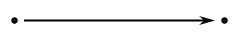
\includegraphics[width=0.8\linewidth]{figures/intro/scg/arcs/const/scg_const_perm_positive2.png}} & \parbox[|c]{2cm}{\centering\ni} & \parbox[|m]{2cm}{\centering\in} & \parbox[|c]{2cm}{\centering->} & \parbox[|m|]{2cm}{\centering<-} \\
	\hline
	
	\parbox[m|]{4.6cm}{\textit{\\ константная постоянная негативная sc-дуга принадлежности \\}} & \parbox[m|]{3.5cm}{\centering 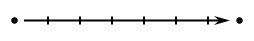
\includegraphics[width=0.8\linewidth]{figures/intro/scg/arcs/const/scg_const_perm_negative2.png}} & \parbox[m]{2cm}{\centering \not\ni} & \parbox[m|]{2cm}{\centering\notin} & \parbox[m|]{2cm}{\centering-|>} & \parbox[m]{2cm}{\centering<|-} \\
	\hline
	
	\parbox[m]{4.6cm}{\textit{\\ константная постоянная нечеткая sc-дуга принадлежности \\}} & \parbox[m]{3.5cm}{\centering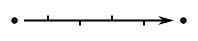
\includegraphics[width=0.8\linewidth]{figures/intro/scg/arcs/const/scg_const_perm_fuzzy2.png}} & \parbox[m]{2cm}{\centering / \ni} & \parbox[m]{2cm}{\centering \in /} & \parbox[m]{2cm}{\centering -/>} & \parbox[m]{2cm}{\centering </-} \\
	\hline
	
	\parbox[m]{4.6cm}{\textit{\\ константная временная позитивная sc-дуга принадлежности \\}} & \parbox[m]{3.5cm}{\centering 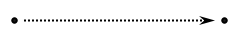
\includegraphics[width=0.8\linewidth]{figures/intro/scg/arcs/const/scg_const_temp_positive2.png}} & \parbox[m]{2cm}{\centering \sim \ni} & \parbox[m]{2cm}{\centering \in \sim} & \parbox[m]{2cm}{\centering \sim>} & \parbox[m]{2cm}{\centering <\sim} \\
	\hline
	
	\parbox[m]{4.6cm}{\textit{\\ константная временная негативная sc-дуга принадлежности \\}} & \parbox[m]{3.5cm}{\centering 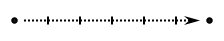
\includegraphics[width=0.8\linewidth]{figures/intro/scg/arcs/const/scg_const_temp_negative2.png}} & \parbox[m]{2cm}{\centering \sim \not\ni} & \parbox[m]{2cm}{\centering \notin \sim} & \parbox[m]{2cm}{\centering \sim|>} & \parbox[m]{2cm}{\centering <|\sim} \\
	\hline
	
	\parbox[m]{4.6cm}{\textit{\\ константная временная нечеткая sc-дуга принадлежности \\}} & \parbox[m]{3.5cm}{\centering 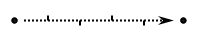
\includegraphics[width=0.8\linewidth]{figures/intro/scg/arcs/const/scg_const_temp_fuzzy2.png}} & \parbox[m]{2cm}{\centering \sim / \ni}  & \parbox[m]{2cm}{\centering \in/\sim} & \parbox[m]{2cm}{\centering \sim/>} & \parbox[m]{2cm}{\centering </\sim} \\
	\hline
	
	\parbox[m]{4.6cm}{\textit{\\ переменная постоянная позитивная sc-дуга принадлежности \\}} & \parbox[m]{3.5cm}{\centering 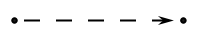
\includegraphics[width=0.8\linewidth]{figures/intro/scg/arcs/var/scg_var_perm_positive2.png}} & \parbox[m]{2cm}{\centering \textunderscore \ni} & \parbox[m]{2cm}{\centering \textunderscore \in} & \parbox[m]{2cm}{\centering \textunderscore->} & \parbox[m]{2cm}{\centering <-\textunderscore} \\
	\hline
	
	\parbox[m]{4.6cm}{\textit{\\ переменная постоянная негативная sc-дуга принадлежности \\}} & \parbox[m]{3.5cm}{\centering 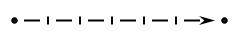
\includegraphics[width=0.8\linewidth]{figures/intro/scg/arcs/var/scg_var_perm_negative2.png}} & \parbox[m]{2cm}{\centering \textunderscore \not\ni} & \parbox[m]{2cm}{\centering \notin \textunderscore} & \parbox[m]{2cm}{\centering \textunderscore-|>} & \parbox[m]{2cm}{\centering <|-\textunderscore} \\
	\hline
	
	\parbox[m]{4.6cm}{\textit{\\ переменная постоянная нечеткая sc-дуга принадлежности \\}} & \parbox[m]{3.5cm}{\centering 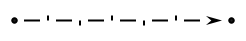
\includegraphics[width=0.8\linewidth]{figures/intro/scg/arcs/var/scg_var_perm_fuzzy2.png}} & \parbox[m]{2cm}{\centering \textunderscore /\ni} & \parbox[m]{2cm}{\centering \in/\textunderscore} & \parbox[m]{2cm}{\centering \textunderscore-/>} & \parbox[m]{2cm}{\centering </-\textunderscore} \\
	\hline
	
	\parbox[m]{4.6cm}{\textit{\\ переменная временная позитивная sc-дуга принадлежности \\}} & \parbox[m]{3.5cm}{\centering 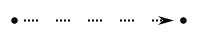
\includegraphics[width=0.8\linewidth]{figures/intro/scg/arcs/var/scg_var_temp_positive2.png}} & \parbox[m]{2cm}{\centering \textunderscore \sim \ni} & \parbox[m]{2cm}{\centering \in \sim \textunderscore} & \parbox[m]{2cm}{\centering \textunderscore \sim >} & \parbox[m]{2cm}{\centering < \sim \textunderscore} \\
	\hline
	
	\parbox[m]{4.6cm}{\textit{\\ переменная временная негативная sc-дуга принадлежности \\}} & \parbox[m]{3.5cm}{\centering 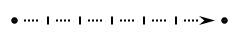
\includegraphics[width=0.8\linewidth]{figures/intro/scg/arcs/var/scg_var_temp_negative2.png}} & \parbox[m]{2cm}{\centering \textunderscore \sim \not$\ni$} & \parbox[c]{2cm}{\centering \notin \sim \textunderscore} & \parbox[m]{2cm}{\centering \textunderscore \sim |>} & \parbox[m]{2cm}{\centering <| \sim \textunderscore} \\
	\hline
	
	\parbox[m]{4.6cm}{\textit{\\переменная временная нечеткая sc-дуга принадлежности\\}} & \parbox[m]{3.5cm}{\centering 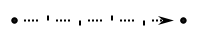
\includegraphics[width=0.8\linewidth]{figures/intro/scg/arcs/var/scg_var_temp_fuzzy2.png}} & \parbox[m]{2cm}{\centering \textunderscore \sim / \ni} & \parbox[m]{2cm}{\centering \in/\sim\textunderscore} & \parbox[m]{2cm}{\centering \textunderscore \sim />} & \parbox[m]{2cm}{\centering </\sim \textunderscore} \\
	\hline
	
	\parbox[m]{4.6cm}{\textit{\\метапеременная постоянная позитивная sc-дуга принадлежности\\}} & \parbox[m]{3.5cm}{\centering 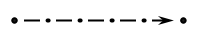
\includegraphics[width=0.8\linewidth]{figures/intro/scg/arcs/meta/scg_metavar_perm_positive2.png}} & \parbox[m]{2cm}{\centering\textunderscore \textunderscore\ni} & \parbox[m]{2cm}{\centering\in\textunderscore\textunderscore} & \parbox[m]{2cm}{\centering\textunderscore\textunderscore->} & \parbox[m]{2cm}{\centering <-\textunderscore\textunderscore} \\
	\hline
	
	\parbox[m]{4.6cm}{\textit{\\ метапеременная постоянная негативная sc-дуга принадлежности \\}} & \parbox[m]{3.5cm}{\centering 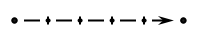
\includegraphics[width=0.8\linewidth]{figures/intro/scg/arcs/meta/scg_metavar_perm_negative2.png}} & \parbox[m]{2cm}{\centering \textunderscore\textunderscore \not\ni} & \parbox[m]{2cm}{\centering \notin\textunderscore\textunderscore} & \parbox[m]{2cm}{\centering \textunderscore\textunderscore-|>} & \parbox[m]{2cm}{\centering <|-\textunderscore\textunderscore} \\
	\hline
	
	\parbox[m]{4.6cm}{\textit{\\ метапеременная постоянная нечеткая sc-дуга принадлежности \\}} & \parbox[m]{3.5cm}{\centering 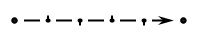
\includegraphics[width=0.8\linewidth]{figures/intro/scg/arcs/meta/scg_metavar_perm_fuzzy2.png}} & \parbox[m]{2cm}{\centering\textunderscore\textunderscore/\ni} & \parbox[m]{2cm}{\centering\in/\textunderscore\textunderscore} & \parbox[m]{2cm}{\centering\textunderscore\textunderscore-/>} & \parbox[m]{2cm}{\centering </-\textunderscore\textunderscore} \\
	\hline
	
	\parbox[m]{4.6cm}{\textit{\\ метапеременная временная позитивная sc-дуга принадлежности \\}} & \parbox[m]{3.5cm}{\centering 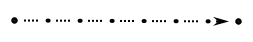
\includegraphics[width=0.8\linewidth]{figures/intro/scg/arcs/meta/scg_metavar_temp_positive2.png}} & \parbox[m]{2cm}{\centering\textunderscore\textunderscore\sim\ni} & \parbox[m]{2cm}{\centering\in\sim\textunderscore\textunderscore} & \parbox[m]{2cm}{\centering\textunderscore\textunderscore\sim>} & \parbox[m]{2cm}{\centering <\sim\textunderscore\textunderscore} \\
	\hline
	
	\parbox[m]{4.6cm}{\textit{\\ метапеременная временная негативная sc-дуга принадлежности \\}} & \parbox[m]{3.5cm}{\centering 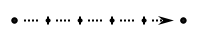
\includegraphics[width=0.8\linewidth]{figures/intro/scg/arcs/meta/scg_metavar_temp_negative2.png}} & \parbox[m]{2cm}{\centering \textunderscore\textunderscore\sim \not\ni} & \parbox[m]{2cm}{\centering\notin\sim\textunderscore\textunderscore} & \parbox[m]{2cm}{\centering\textunderscore\textunderscore\sim|>} & \parbox[m]{2cm}{\centering <|\sim\textunderscore\textunderscore} \\
	\hline
	
	\parbox[m]{4.6cm}{\textit{\\ метапеременная временная нечеткая sc-дуга принадлежности \\}} & \parbox[m]{3.5cm}{\centering 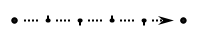
\includegraphics[width=0.8\linewidth]{figures/intro/scg/arcs/meta/scg_metavar_temp_fuzzy2.png}} & \parbox[m]{2cm}{\centering \textunderscore\textunderscore\sim/\ni} & \parbox[m]{2cm}{\centering\in/\sim\textunderscore\textunderscore} & \parbox[m]{2cm}{\centering\textunderscore\textunderscore\sim/>} & \parbox[m]{2cm}{\centering</\sim\textunderscore\textunderscore} \\
	\hline
\end{longtable}
}
%---------------------------------------------
\scnheader{Таблица. Алфавит sc.s-коннекторов, соответствующих sc.g-коннекторам, которые не являются sc.g-дугами принадлежности}
\scneqtable{
\begin{longtable}[l]{|m{6.2cm}|m{2.5cm}|m{2.5cm}|m{2.5cm}|m{2.5cm}|}
	\hline
	\multicolumn{1}{|c}{\parbox[c]{6.2cm}{Изображение \textit{\mbox{sc-коннектора}} в SCg}} &
	\multicolumn{2}{|c}{\parbox[c]{5cm}{Изображение \textit{\mbox{sc.s-коннектора}} в Расширенном алфавите}} &
	\multicolumn{2}{|c|}{\parbox[c]{5cm}{Изображение \textit{\mbox{sc.s-коннектора}} в Базовом алфавите}}
	\hline
	\endhead
	
	\parbox[|c]{6.2cm}{\\\centering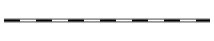
\includegraphics[width=0.8\linewidth]{figures/intro/scs/sc.s-connectors/noorient.png}\\} & \multicolumn{2}{c|}{ \parbox[c]{5cm}{\centering\leftrightarrow}} & \multicolumn{2}{c|}{ \parbox[c]{5cm}{\centering<>}} \\
	\hline
	
	\parbox[c]{6.2cm}{\\\centering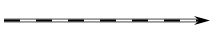
\includegraphics[width=0.8\linewidth]{figures/intro/scs/sc.s-connectors/orient.png} \\} &\parbox[c]{2.5cm}{\\\centering\rightarrow\\} & \parbox[c]{2.5cm}{\\\centering\leftarrow\\} & \parbox[c]{2.5cm}{\\\centering >>\\} & \parbox[c|]{2.5cm}{\\\centering <<\\} \\
	\hline
	
	\parbox[c]{6.2cm}{\\\centering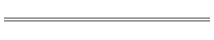
\includegraphics[width=0.8\linewidth]{figures/intro/scs/sc.s-connectors/constPermNoorien.png}\\} & \multicolumn{2}{c|}{\parbox[c]{5cm}{\centering\Leftrightarrow}} & \multicolumn{2}{c|}{\parbox[c]{5cm}{\centering<=>}} \\
	\hline
	
	\parbox[c]{6.2cm}{\\\centering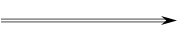
\includegraphics[width=0.8\linewidth]{figures/intro/scs/sc.s-connectors/constPermOrient.png}\\} & \parbox[c]{2.5cm}{\centering\Rightarrow} & \parbox[c]{2.5cm}{\centering\Leftarrow} & \parbox[c]{2.5cm}{\centering =>} & \parbox[c|]{2.5cm}{\centering <=} \\
	\hline
	
	\parbox[c]{6.2cm}{\\\centering
\includegraphics[width=0.8\linewidth]{figures/intro/scs/sc.s-connectors/constTempNoorien.png}\\} & \multicolumn{2}{c|}{\parbox[c]{5cm}{\centering\sim\Leftrightarrow}} & \multicolumn{2}{c|}{\parbox[c|]{5cm}{\centering\sim<=>}} \\
	\hline
	
	\parbox[c]{6.2cm}{\\\centering 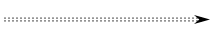
\includegraphics[width=0.8\linewidth]{figures/intro/scs/sc.s-connectors/constTempOrient.png}\\} & \parbox[c]{2.5cm}{\centering\sim\Rightarrow} & \parbox[c]{2.5cm}{\centering\Leftarrow\sim} & \parbox[c]{2.5cm}{\centering\sim=>} & \parbox[c|]{2.5cm}{\centering <=\sim} \\
	\hline
	
	\parbox[c]{6.2cm}{\\\centering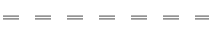
\includegraphics[width=0.8\linewidth]{figures/intro/scs/sc.s-connectors/varPermNoorien.png}\\} & \multicolumn{2}{c|}{\parbox[c]{5cm}{\centering\textunderscore\Leftrightarrow}} & \multicolumn{2}{c|}{\parbox[c|]{5cm}{\centering\textunderscore<=>}} \\
	\hline
	
	\parbox[c]{6.2cm}{\\\centering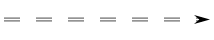
\includegraphics[width=0.8\linewidth]{figures/intro/scs/sc.s-connectors/varPermOrient.png}\\} & \parbox[c]{2.5cm}{\centering\textunderscore\Rightarrow} & \parbox[c]{2.5cm}{\centering\Leftarrow\textunderscore} & \parbox[c]{2.5cm}{\centering\textunderscore=>} & \parbox[c|]{2.5cm}{\centering <=\textunderscore} \\
	\hline
	
	\parbox[c]{6.2cm}{\\\centering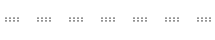
\includegraphics[width=0.8\linewidth]{figures/intro/scs/sc.s-connectors/varTempNoorien.png}\\} & \multicolumn{2}{c|}{\parbox[c]{5cm}{\centering\textunderscore\sim\Leftrightarrow}} & \multicolumn{2}{c|}{\parbox[c]{5cm}{\centering\textunderscore\sim<=>}} \\
	\hline
	
	\parbox[c]{6.2cm}{\\\centering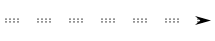
\includegraphics[width=0.8\linewidth]{figures/intro/scs/sc.s-connectors/varTempOrient.png}\\} & \parbox[c]{2.5cm}{\centering\textunderscore\sim\Rightarrow} & \parbox[c]{2.5cm}{\centering\Leftarrow\sim\textunderscore} & \parbox[c]{2.5cm}{\centering\textunderscore\sim=>} & \parbox[c|]{2.5cm}{\centering <=\sim\textunderscore} \\
	\hline
	
	\parbox[c]{6.2cm}{\\\centering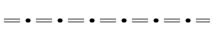
\includegraphics[width=0.8\linewidth]{figures/intro/scs/sc.s-connectors/metaPermNoorien.png}\\} & \multicolumn{2}{c|}{\parbox[c]{5cm}{\centering\textunderscore\textunderscore\Leftrightarrow}} & \multicolumn{2}{c|}{\parbox[c|]{5cm}{\centering\textunderscore\textunderscore<=>}} \\
	\hline
	
	\parbox[c]{6.2cm}{\\\centering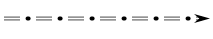
\includegraphics[width=0.8\linewidth]{figures/intro/scs/sc.s-connectors/metaPermOrient.png}\\} & \parbox[c]{2.5cm}{\centering\textunderscore\textunderscore\Rightarrow} & \parbox[c]{2.5cm}{\centering\Leftarrow\textunderscore\textunderscore} & \parbox[c]{2.5cm}{\centering\textunderscore\textunderscore=>} & \parbox[c|]{2.5cm}{\centering <=\textunderscore\textunderscore} \\
	\hline
	
	\parbox[c]{6.2cm}{\\\centering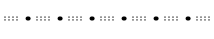
\includegraphics[width=0.8\linewidth]{figures/intro/scs/sc.s-connectors/metaTempNoorien.png}\\} & \multicolumn{2}{c|}{\parbox[c]{5cm}{\centering\textunderscore\textunderscore\sim\Leftrightarrow}} & \multicolumn{2}{c|}{\parbox[c]{5cm}{\centering\textunderscore\textunderscore\sim<=>}} \\
	\hline
	
	\parbox[c]{6.2cm}{\\\centering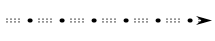
\includegraphics[width=0.8\linewidth]{figures/intro/scs/sc.s-connectors/metaTempOrient.png}\\} & \parbox[c]{2.5cm}{\centering\textunderscore\textunderscore\sim\Rightarrow} & \parbox[c]{2.5cm}{\centering\Leftarrow\sim\textunderscore\textunderscore} & \parbox[c]{2.5cm}{\centering\textunderscore\textunderscore\sim\Rightarrow} & \parbox[c|]{2.5cm}{\centering\Leftarrow\sim\textunderscore\textunderscore} \\
	\hline
	
	\parbox[c]{6.2cm}{\\\centering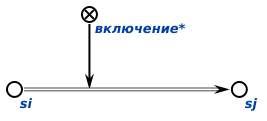
\includegraphics[width=0.8\linewidth]{figures/intro/scs/sc.s-connectors/examples/scs_transf_inclusion_const.png}\\} & \parbox[c]{2.5cm}{\centering\supseteq} & \parbox[c]{2.5cm}{\centering\subseteq} & \multicolumn{2}{c|}{\parbox[c]{5cm}{}} \\
	\hline
	
	\parbox[c]{6.2cm}{\\\centering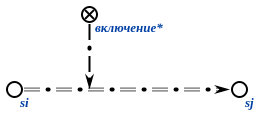
\includegraphics[width=0.8\linewidth]{figures/intro/scs/sc.s-connectors/examples/scs_transf_inclusion_meta.png}\\} & \parbox[c]{2.5cm}{\centering\textunderscore\supseteq} & \parbox[c]{2.5cm}{\centering\subseteq\textunderscore} & \multicolumn{2}{c|}{\parbox[c|]{5cm}{\centering}} \\
	\hline
	
	\parbox[c]{6.2cm}{\\\centering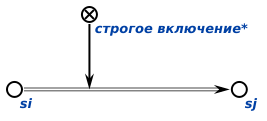
\includegraphics[width=0.8\linewidth]{figures/intro/scs/sc.s-connectors/examples/scs_transf_strict_inclusion_const.png}\\} & \parbox[c]{2.5cm}{\centering\supset} & \parbox[c]{2.5cm}{\centering\subset} & \multicolumn{2}{c|}{\parbox[c|]{5cm}{}} \\
	\hline
	
	\parbox[c]{6.2cm}{\\\centering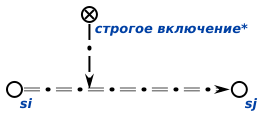
\includegraphics[width=0.8\linewidth]{figures/intro/scs/sc.s-connectors/examples/scs_transf_strict_inclusion_meta.png}\\} & \parbox[c]{2.5cm}{\centering\textunderscore\supset} & \parbox[c]{2.5cm}{\centering\subset\textunderscore} & \multicolumn{2}{c|}{\parbox[c|]{5cm}{}} \\
	\hline
	
	\parbox[c]{6.2cm}{\\\centering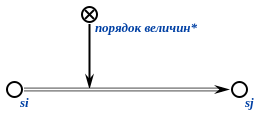
\includegraphics[width=0.8\linewidth]{figures/intro/scs/sc.s-connectors/examples/scs_transf_value_order_const.png}\\} & \parbox[c]{2.5cm}{\centering\geq} & \parbox[c]{2.5cm}{\centering\leq} & \multicolumn{2}{c|}{\parbox[c|]{5cm}{}} \\
	\hline
	
	\parbox[c]{6.2cm}{\\\centering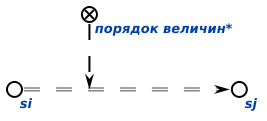
\includegraphics[width=0.8\linewidth]{figures/intro/scs/sc.s-connectors/examples/scs_transf_value_order_var.png}\\} & \parbox[c]{2.5cm}{\centering\textunderscore\geq} & \parbox[c]{2.5cm}{\centering\textunderscore\leq} & \multicolumn{2}{c|}{\parbox[c]{5cm}{}}  \\
	\hline
	
	\parbox[c]{6.2cm}{\\\centering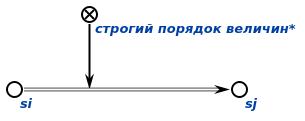
\includegraphics[width=0.8\linewidth]{figures/intro/scs/sc.s-connectors/examples/scs_transf_value_strict_order_const.png}\\} & \parbox[c]{2.5cm}{\centering >} & \parbox[c]{2.5cm}{\centering <} & \multicolumn{2}{c|}{\parbox[c]{5cm}{}} \\
	\hline
	
	\parbox[c]{6.2cm}{\\\centering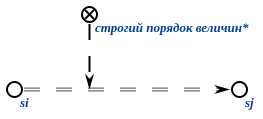
\includegraphics[width=0.8\linewidth]{figures/intro/scs/sc.s-connectors/examples/scs_transf_value_strict_order_var.png}\\} & \parbox[c]{2.5cm}{\centering\textunderscore>} & \parbox[c]{2.5cm}{\centering <\textunderscore} & \multicolumn{2}{c|}{\parbox[c]{5cm}{}} \\
	\hline
	
	\parbox[c]{6.2cm}{\\\centering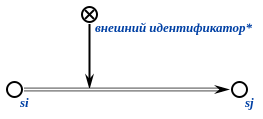
\includegraphics[width=0.8\linewidth]{figures/intro/scs/sc.s-connectors/examples/scs_transf_external_idtf_const.png}\\} & \multicolumn{2}{c|}{\parbox[c]{5cm}{\centering :=}} & \multicolumn{2}{c|}{\parbox[c]{5cm}{}} \\
	\hline
	
	\parbox[c]{6.2cm}{\\\centering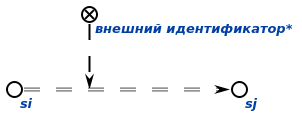
\includegraphics[width=0.8\linewidth]{figures/intro/scs/sc.s-connectors/examples/scs_transf_external_idtf_var.png}\\} & \multicolumn{2}{c|}{\parbox[c]{5cm}{\centering\textunderscore:=}} & \multicolumn{2}{c|}{\parbox[c]{5cm}{}} \\
	\hline
	
	\parbox[c]{6.2cm}{\\\centering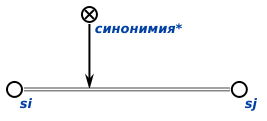
\includegraphics[width=0.8\linewidth]{figures/intro/scs/sc.s-connectors/examples/scs_transf_synonymy_const.png}\\} & \multicolumn{2}{c|}{\parbox[c]{5cm}{\centering =}} & \multicolumn{2}{c|}{\parbox[c]{5cm}{}} \\
	\hline
	
	\parbox[c]{6.2cm}{\\\centering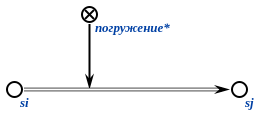
\includegraphics[width=0.8\linewidth]{figures/intro/scs/sc.s-connectors/examples/scs_transf_insertion_const.png}\\} & \parbox[c]{2.5cm}{\centering\supset=} & \parbox[c]{2.5cm}{\centering = \subset} &  \multicolumn{2}{c|}{\parbox[c]{5cm}{}}  \\
	\hline
\end{longtable}
}

\bigskip
\scnendstruct \scnendsegmentcomment{Описание sc.s-разделителей и sc.s-ограничителей}

\scnsegmentheader{Описание sc.s-предложений}
\scnstartsubstruct

\scnheader{sc.s-предложение}
\scnidtf{минимальный семантически целостный фрагмент sc.s-текста}
\scnidtf{минимальный sc.s-текст}
\scnsubset{sc.s-текст}
\scnsuperset{простое sc.s-предложение\\
    \scnaddlevel{1}
    \scnidtf{минимальное sc.s-предложение}
    \scnexplanation{\textit{sc.s-предложение}, (1) \uline{состоящее} или из двух \textit{sc-идентификаторов}, соединенных между собой \textit{\mbox{sc.s-коннектором}}, или из трех \textit{sc-идентификаторов}, разделенных \textit{sc.s-разделителями, изображающими связь инцидентности sc-элементов}, и (2) завершающееся \textit{двойной точкой с запятой}}
    \scnnote{Нетрудно заметить, что простые sc.s-предложения по сути аналогичны триплетам языка RDF (\mbox{RDF-триплетам}), за тем исключением, что \textit{простое sc.s-предложение} можно "развернуть"\ при помощи \textit{Операции конверсии sc.s-предложений*} не меняя при этом его смысл, а RDF-триплет нельзя. Это является одной из причин, по которой, в отличие от RDF-триплетов, в простых \mbox{sc.s-предложениях} \textit{\mbox{sc.s-коннекторы}} и \textit{\mbox{sc.s-разделители}, изображающие связь инцидентности \mbox{sc-элементов}} не могут быть опущены, поскольку они в том числе показывают направление изображаемой ими связи между sc-элементами.}
\scnrelfromlist{пример}{
    \scnfileitem{\textit{многоугольник} $\supset$ \textit{треугольник}}
    \scnaddlevel{1}
    \scnrelboth{семантическая эквивалентность}{\scnfilescg{figures/intro/scs/inclusion.png}}
    \scnaddlevel{-1};
    \scnfileitem{\textit{сторона*} $\ni$ (\textit{Четырехугк(ТчкА\char59ТчкВ\char59ТчкС\char59ТчкD)} $\Rightarrow$ \textit{Отр(ТчкВ\char59ТчкС)})\char59\char59}
    \scnaddlevel{1}
    \scnrelboth{семантическая эквивалентность}{\scnfilescg{figures/intro/scs/side.png}}
    \scnaddlevel{-1};
    \scnfileitem{\textit{Si} |- \textit{ai} >| \textit{ei}}
    \scnaddlevel{1}
    \scnrelboth{семантическая эквивалентность}{\scnfilescg{figures/intro/scs/inclusion_incident.png}}
    \scnaddlevel{-1}
    }
\scnaddlevel{-1}}
\scnnote{Признаком завершения любого \textit{sc.s-предложения}, т.е. последними его символами является \textit{двойная точка с запятой}, которую, следовательно, можно считать разделителем \textit{sc.s-предложений}.}
\scnrelfromlist{заданная операция}{Операция конверсии sc.s-предложения*\\
    \scnaddlevel{1}
    \scnsubset{синтаксическая трансформация*}
    \scnexplanation{Каждое \textit{sc.s-предложение} (в том числе, и \textit{простое sc.s-предложение}) можно преобразовать в семантически эквивалентное ему \textit{sc.s-предложение} путем конверсии ("разворота") цепочки компонентов \textit{sc.s-предложения}. Так, например, при конверсии ("развороте") простого \textit{\mbox{sc.s-предложения}} (1) первый его \textit{\mbox{sc-идентификатор}} (первый компонент этого \textit{\mbox{sc.s-предложения}}) становится третьим компонентом конвертированного\textit{ \mbox{sc.s-предложения}}, (2) второй его \textit{\mbox{sc-идентификатор}} (третий компонент исходного \textit{\mbox{sc.s-предложения}}) становится первым компонентом "конвертированного"\ \textit{\mbox{sc.s-предложения}} и (3) второй компонент исходного \textit{\mbox{sc.s-предложения}} (\textit{\mbox{sc.s-коннектор}} или \textit{\mbox{sc.s-разделитель}, изображающий связь инцидентности \mbox{sc-элементов}}, соединяющий указанные выше компоненты) остается вторым компонентом конвертированного \textit{\mbox{sc.s-предложения}}, но меняет направленность ("$\ni$"\ заменяется на "$\in$"\ и наоборот, "$\supset$"\ на "$\subset$"\ и наоборот, "$\Rightarrow$"\ на "$\Leftarrow$"\ и наоборот и т.д.)}
    \scnnote{Можно говорить не только о конверсии sc.s-предложения, но и о конверсии sc.s-коннектора, о конверсии sc.s-разделителя, изображающего связь инцидентности sc.s-элементов.}
    \scnrelfrom{sc.s-текст до трансформации}{\scnfilelong{\textit{треугольник $\ni$ Треуг(ТчкВ\char59ТчкС\char59ТчкD)}\char59\char59}}
    \scnrelfrom{sc.s-текст после трансформации}{\scnfilelong{\textit{Треуг(ТчкВ\char59ТчкС\char59ТчкD) $\in$ треугольник}\char59\char59}}
	\scnaddlevel{1}
    \scnrelboth{семантическая эквивалентность}{\scnfilescg{figures/intro/scs/conversion.png}}
    \scnaddlevel{-2}
;Операция присоединения sc.s-предложения*\\
    \scnaddlevel{1}
    \scnsubset{синтаксическая трансформация*}
    \scnidtf{Операция соединения двух sc.s-предложений при совпадении последнего компонента первого предложения с первым компонентом второго*}
    \scnexplanation{В результате выполнения данной операции:
    \begin{scnitemize}
        \item первый компонент второго sc.s-предложения удаляется\char59
        \item оставшаяся часть второго предложения окружается sc.s-ограничителем присоединенных предложений ("(*"\ и "*)"). Разделитель sc.s-предложений (";;") также попадает внутрь указанного ограничителя\char59
        \item полученная конструкция помещается между последним компонентом первого предложения и разделителем sc.s-предложений, которым заканчивалось первое предложение\char59
        \item второе предложение, таким образом, становится присоединенным sc.s-предложением.
    \end{scnitemize}
    Аналогичным образом к любому присоединенному sc.s-предложению могут "пристыковываться"\ другие присоединенные sc.s-предложения, в общем случае уровень такой вложенности не ограничен.
    }
    \scnaddlevel{-1}
;Операция слияния sc.s-предложений*\\
    \scnaddlevel{1}
    \scnsubset{синтаксическая трансформация*}
    \scnidtf{Операция присоединения простого sc.s-предложения к sc.s-предложению, у которого последний sc.s-коннектор совпадает с sc.s-коннектором простого sc.s-предложения, а предшествующий указанному sc.s-коннектору sc-идентификатор совпадает с первым sc-идентификатором простого sc.s-предложения*}
    \scnexplanation{В результате выполнения этой операции совпадающие sc-идентификаторы и sc.s-коннекторы соединяемых sc.s-предложений "склеиваются"\ , а последние sc-иден\-ти\-фи\-ка\-то\-ры соединяемых \textit{sc.s-предложений} становятся последними компонентами объединенного \textit{sc.s-предложения},
    разделенными \textit{точкой с запятой}. Аналогичным образом можно присоединять сколько угодно простых \textit{sc.s-предложений}.}
    \scnaddlevel{-1}
;Операция разложения sc.s-предложений на простые sc.s-предложения*\\
    \scnaddlevel{1}
    \scnsubset{синтаксическая трансформация*}
    \scnexplanation{Каждое \textit{sc.s-предложение} можно разложить на множество \textit{простых sc.s-предложений}, т.е. представить в виде последовательности \textit{простых sc.s-предложений}.}
    \scnaddlevel{-1}
;Операция разложения sc.s-предложений на простые sc.s-предложения с sc.s-разделителем, изображающим связь инцидентности sc-элементов*\\
    \scnaddlevel{1}
    \scnsubset{синтаксическая трансформация*}
    \scnexplanation{Каждое \textit{sc.s-предложение} (в том числе и \textit{простое sc.s-предложение} с \textit{sc.s-коннектором}) можно представить в виде семантически эквивалентной последовательности \textit{простых \mbox{sc.s-предложений}} с \textit{sc.s-разделителем, изображающим связь инцидентности \mbox{sc-элементов}}.}
    \scnnote{Данная операция осуществляет \uline{однозначное} (!) формирование множества \textit{простых \mbox{sc.s-предложений}} указанного вида.}
    \scnaddlevel{-1}
    }

\newpage
\scnheader{sc.s-предложение}
\scnnote{Операции, заданные на множестве \textit{sc.s-предложений} можно разделить на три группы:
    \begin{scnitemize}
        \item группа операций конверсии \textit{sc.s-предложений}, состоящая из одной операции;
        \item группа операций соединения \textit{sc.s-предложений};
        \item группа операций декомпозиции \textit{sc.s-предложений} и, в частности, операций разложения \textit{sc.s-предложений}.
    \end{scnitemize}
Очевидно, что операции соединения \textit{sc.s-предложений} и операции декомпозиции \textit{sc.s-предложений} являются обратными друг другу операциями.}
\scnaddlevel{-1}

\scnheader{Описание примеров выполнения операций, заданных на множестве sc.s-предложений}
\scnstartsubstruct

\bigskip

\scnfilelong{\textit{треугольник $\ni$ Треугк(ТчкВ\char59ТчкС\char59ТчкD)}\char59\char59}
\scnrelfrom{Операция конверсии sc.s-предложения}{\scnfilelong{\textit{Треугк(ТчкВ\char59ТчкС\char59ТчкD) $\in$ треугольник}\char59\char59}}
\scnaddlevel{1}
\scnrelboth{семантическая эквивалентность}{\scnfilescg{figures/intro/scs/conversion.png}}
\scnaddlevel{-1}

\bigskip\bigskip

{\scnfilelong{\textit{треугольник $\ni$ Треугк(ТчкВ\char59ТчкС\char59ТчкD)\char59\char59
\newline
Треугк(ТчкВ\char59ТчкС\char59ТчкD) $\Rightarrow$ сторона*:включение*: Отр(ТчкВ\char59ТчкC)\char59\char59}}}
\scnrelfrom{Операция присоединения sc.s-предложения}{\scnfilelong{\textit{треугольник $\ni$ Треугк(ТчкВ\char59ТчкС\char59ТчкD) (* $\Rightarrow$ сторона*:включение*:Отр(ТчкВ\char59ТчкС)\char59\char59*) }\char59\char59}}
\scnaddlevel{1}
\scnrelboth{семантическая эквивалентность}{\scnfilescg{figures/intro/scs/joining_sentences.png}}
\scnaddlevel{-1}

\bigskip\bigskip

\scnfilelong{\textit{сторона* $\ni$ (Треугк(ТчкВ\char59Тчк С\char59ТчкD) $\Rightarrow$ Отр(ТчкВ\char59ТчкС))\char59\char59
\newline
сторона* $\ni$ (Треугк(ТчкВ\char59Тчк С\char59ТчкD) $\Rightarrow$ Отр(ТчкC\char59ТчкD))\char59\char59}}
\scnrelfrom{Операция слияния sc.s-предложений}{\scnfilelong{\textit{сторона* $\ni$ ((Треугк(ТчкВ\char59ТчкС\char59ТчкD) $\Rightarrow$ Отр(ТчкВ\char59ТчкС))\char59(Треуг(ТчкВ\char59ТчкС\char59ТчкD) $\Rightarrow$ Отр(ТчкC\char59ТчкD)))\char59\char59}}}
\scnaddlevel{1}
\scnrelfrom{синтаксическая трансформация}{\scnfilelong{\textit{Треугк(ТчкВ\char59ТчкС\char59ТчкD)}$\Rightarrow$\textit{сторона*}: \textit{Отр(ТчкВ\char59ТчкС)}\char59\textit{Отр(ТчкС\char59ТчкD)}\char59\char59}}
\scnrelboth{семантическая эквивалентность}{\scnfilescg{figures/intro/scs/joining_sentence.png}}
\scnaddlevel{-1}

\bigskip\bigskip

\newpage
{\scnfilelong{\textit{Треугк(ТчкВ\char59ТчкС\char59ТчкD) $\Rightarrow$ сторона*:включение*:Отр(ТчкВ\char59ТчкС)\char59\char59}}}
\scnrelfrom{Операция разложения sc.s-предложений на простые sc.s-предложения}{\scnfilelong{\textit{сторона* $\ni$ (Треугк(ТчкВ\char59ТчкС\char59ТчкD) $\Rightarrow$ Отр(ТчкВ\char59ТчкС))\char59\char59
\newline включение* $\ni$ (Треугк(ТчкВ\char59ТчкС\char59ТчкD) $\Rightarrow$ Отр(ТчкВ\char59ТчкС))\char59\char59}}}
\scnaddlevel{1}
\scnrelboth{семантическая эквивалентность}{\scnfilescg{figures/intro/scs/dividing_sentences.png}}
\scnaddlevel{-1}

\bigskip\bigskip

{\scnfilelong{\textit{треугольник $\ni$ Треугк(ТчкВ\char59ТчкC\char59ТчкD)}}}
\scnrelfrom{Операция разложения sc.s-предложений на простые sc.s-предложения с sc.s-разделителем, изображающим связь инцидентности sc-элементов}{\scnfilelong{\textit{треугольник |- ai >| Треугк(ТчкВ\char59ТчкС\char59ТчкD)\char59\char59
\newline
константный постоянный sc-узел, обозначающий класс $\ni$ треугольник\char59\char59
\newline
константная постоянная позитивная sc-дуга принадлежности $\ni$ ai\char59\char59
\newline
константный постоянный sc-узел общего вида $\ni$ Треугк(ТчкВ\char59ТчкC\char59ТчкD)\char59\char59}}}
\scnaddlevel{1}
\scnrelboth{семантическая эквивалентность}{\scnfilescg{figures/intro/scs/dividing_sentences_incident.png}}
\scnaddlevel{-1}

\scnendstruct

\scnheader{присоединенное sc.s-предложение}
\scnidtf{встроенное sc.s-предложение}
\scnexplanation{Присоединенные sc.s-предложения используются для того, чтобы продолжить спецификацию какого-либо sc-элемента, sc-идентификатор которого является последним компонентом в рамках какого-либо sc.s-предложения, не начиная при этом нового sc.s-предложения и, таким образом, не дублируя указанный \mbox{sc-идентификатор}. Внутрь присоединенных sc.s-предложений также могут встраиваться другие присоединенные sc.s-предложения, в общем случае уровень вложенности таких предложений не ограничен. Таким образом присоединенные sc.s-предложения описывают "ветвление"\ sc.s-предложений, при этом точками такого "ветвления"\ выступают sc-идентификаторы, входящие в состав этих sc.s-предложений.

Благодаря введению присоединенных sc.s-предложений появляется возможность любой sc-текст изобразить в виде одного sc.s-предложения, содержащего необходимое количество присоединенных sc.s-предложений. Таким образом, SCs-код по выразительной мощности становится эквивалентным SCn-коду.}

\scnheader{sc.s-предложение}
\scntext{денотационная семантика}{С семантической точки зрения \textit{sc.s-предложение} представляет собой описание некоторого \uline{маршрута} в соответствующем sc-тексте, который является графовой структурой специального вида и структура которого описывается (изображается) с помощью \textit{sc.s-предложений}. Указанный маршрут "проводится"\ по sc-коннекторам и по связям инцидентности sc-элементов, если маршрут проходит через инцидентные sc-коннекторы. В описании указанного маршрута могут дополнительно указываться множества (чаще всего отношения), которым принадлежат sc-коннекторы, входящие в описываемый маршрут. Кроме того, указанный маршрут в начале и/или в конце может иметь разветвления, когда какой-либо sc-элемент \uline{одинаково} инцидентен нескольким \uline{однотипным} sc-коннекторам, соединяющим указанный sc-элемент с некоторыми другими sc-элементами.

Таким образом каждое указанное разветвление состоит из неограниченного числа ветвей, каждая из которых состоит из одного sc-коннектора и одного связываемого им sc-элемента.}

\scnheader{компонент sc.s-предложения*}
\scnexplanation{Каждое \textit{sc.s-предложение} представляет собой последовательность (1) \textit{sc-идентификаторов}, \mbox{(2) \textit{sc.s-коннекторов}} или \textit{sc.s-разделителей}, изображающих связь инцидентности \textit{sc-элементов}, (3) \textit{точек с запятыми}, (4) \textit{ограничителей присоединенных sc.s-предложений}, завершаемая \textit{двойной точкой с запятой}. При этом непосредственно соседствовать друг с другом не могут ни \textit{\mbox{sc-идентификаторы}}, ни \textit{\mbox{sc.s-коннекторы}}, ни, очевидно, \textit{точки с запятыми} и \textit{ограничители присоединенных sc.s-предложений}.\\
Между \textit{sc-идентификаторами} в рамках \textit{sc.s-предложения} может находиться либо \textit{точка с запятой}, либо \textit{sc.s-коннектор}, либо \textit{sc.s-разделитель}, изображающий связь инцидентности \textit{sc-элементов}. Слева и справа от \textit{sc.s-коннектора} и от \textit{sc.s-разделителя}, изображающего связь инцидентности \textit{sc-элементов}, должны находиться \textit{sc-идентификаторы}.

Указанные \textit{sc-идентификаторы}, \textit{sc.s-коннекторы} и \textit{sc.s-разделители}, изображающие связь инцидентности \textit{sc-элементов}, считаются компонентами соответствующего \textit{sc.s-предложения}. Понятие "быть компонентом sc.s-предложения"\ является относительным понятием (отношением), т.к. в состав некоторых компонентов \textit{sc.s-предложения} (в состав \textit{sc-идентификаторов}, являющихся \textit{sc.s-выражениями}, ограничиваемыми фигурными или квадратными скобками) могут входить других \textit{sc.s-предложения}, состоящие из своих компонентов.}
\scnrelfrom{первый домен}{sc.s-предложение}
\scnrelfrom{второй домен}{{\normalfont (} sc-идентификатор $\cup$ sc.s-разделитель $\cup$ sc.s-ограничитель {\normalfont )}}

\scnheader{sc.s-модификатор*}
\scnsubset{компонент sc.s-предложения*}
\scnexplanation{Это дополнительный вид компонентов \textit{sc.s-предложений}. Каждый \textit{sc.s-модификатор}, являющийся компонентом некоторого \textit{sc.s-предложения}, представляет собой \textit{sc-идентификатор}, обозначающий множество (чаще всего, отношение), которому принадлежит sc-коннектор, изображенный \textit{sc.s-коннектором}, который предшествует указанному \textit{sc-идентификатору}. Признаком \textit{sc.s-модификатора} является \textit{двоеточие} (или \textit{двойное двоеточие}), которое ставится после \textit{sc.s-модификатора} и отделяет его либо от следующего за ним другого \textit{sc.s-модификатора} для этого же \textit{sc.s-коннектора}, либо от следующего за ним \textit{sc-идентификатора}, соответствующего sc-элементу, который инцидентен sc-коннектору, изображенному \textit{sc.s-коннектором}, находящимся левее рассматриваемого \textit{sc-идентификатора} после одного или нескольких \textit{sc.s-модификаторов}. Обычное ("одинарное") \textit{двоеточие} обозначает, что sc-элемент, изображенный соответствующим \mbox{sc.s-модификатором}, связан с sc-коннектором, изображенным левее этого \mbox{sc.s-модификатора}, \textit{базовой \mbox{sc-дугой}} (\textit{константной постоянной позитивной \mbox{sc-дугой} принадлежности}), \textit{двойное двоеточие} обозначает, что указанные элементы связаны \textit{переменной постоянной позитивной \mbox{sc-дугой} принадлежности}.}
\scnrelfromlist{пример}{
    \scnfileitem{\textit{Четырехугк(ТчкА;ТчкВ;ТчкС;ТчкD)} $\Rightarrow$ \textit{сторона*} : \textit{включение*} : \textit{Отр(ТчкВ;ТчкС)};; }\\
    \scnaddlevel{1}
    \scnrelboth{семантическая эквивалентность}{\scnfilescg{figures/intro/scs/modifier.png}}
    \scnaddlevel{-1}
    \newpage;
    \scnfileitem{\textit{Треугк(ТчкА;ТчкВ;ТчкС)} $\_\Rightarrow$ \textit{сторона*} :: \textit{\_s};; }\\
    \scnaddlevel{1}
    \scnrelboth{семантическая эквивалентность}{\scnfilescg{figures/intro/scs/modifier_var.png}}
    \scnaddlevel{-1}
    }

\scnheader{sc.s-текст}
\scnidtf{конкатенация \textit{sc.s-предложений}}
\scnidtf{последовательность \textit{sc.s-предложений}, разделяемых \textit{двойными точками с запятой}}
\scnsuperset{максимальный исходный sc.s-текст}
    \scnaddlevel{1}
    \scnidtf{конкатенция \textit{sc.s-предложений}, слева и справа от которой отсутствуют какие-либо символы SCs-кода}
    \scnaddlevel{-1}
\scnsuperset{максимальный sc.s-текст, включенный в структуру}
    \scnaddlevel{1}
    \scnidtf{конкатенция всех \textit{sc.s-предложений}, входящих в состав \textit{sc.s-выражения структуры}}
    \scnsuperset{sc.s-текст, включенный в структуру}
        \scnaddlevel{1}
        \scnidtf{часть цепочки \textit{sc.s-предложений}, входящих в состав максимального sc.s-текста, включенного в структуру}
        \scnsuperset{sc.s-предложение, включенное в структуру}
    \scnaddlevel{-2}
\scnnote{\textit{sc.s-предложение} является минимальным sc.s-текстом.}
\scntext{свойство}{Смысл sc.s-текста (а также \textit{sc.s-текста, включенного в структуру} не зависит от порядка \textit{\mbox{sc.s-предложений}} в этих sc-текстах. Т.е. перестановка \textit{\mbox{sc.s-предложений}} в рамках таких \mbox{sc.s-текстов} смысла этих \mbox{sc.s-текстов} не меняет (т.е. приводит к семантически эквивалентным \mbox{sc.s-текстам}), но сильно влияет на трудоемкость человеческого восприятия (на "читабельность") этих текстов.}
\scnrelfrom{пример}{\scnfilelong{
		\textit{материальный объект} $\ni$ \textit{Земля} (* => \textit{вращаться вокруг}*: \textit{спутник}*: \textit{Луна};;*);;\\
		\textit{материальный объект} $\ni$ \textit{Луна}(* => \textit{основной идентификатор}*: [Moon] (* <- \textit{Английский язык};; *); [Луна] (* <- \textit{Русский язык};; *);; *);;\\
		\textit{материальный объект} $\ni$ \textit{Солнце} (* => \textit{вращаться вокруг}*: \textit{Земля}; \textit{Марс};; *);;\\
		\textit{материальный объект} $\ni$ \textit{Марс};;}
}    
\scnaddlevel{1}
\scnrelfrom{семантическая эквивалентность}{ \scnfilescg{figures/intro/scs/scs_text_example.png}}
\scnaddlevel{-1}
    
\bigskip
\scnendstruct \scnendsegmentcomment{Завершили Описание sc.s-предложений}

\scnsegmentheader{Описание Ядра SCs-кода и различных направлений его расширения}
\scnstartsubstruct

\scnheader{Ядро SCs-кода}
\scnidtf{Подъязык SCs-кода, который использует минимальный набор синтаксических средств, но при этом имеет семантическую мощность, эквивалентную мощности SCs-кода в целом}
\scntext{принципы, лежащие в основе}{В Ядре SCs-кода:
\begin{scnitemize}
    \item используются только \textit{простые sc-идентификаторы}, в том числе \textit{sc-идентификаторы внешних файлов ostis-систем} (sc-выражения не используются);
    \item используются только \textit{sc.s-разделители, изображающие связь инцидентности sc-элементов}, а также sc.s-коннектор, изображающий константную  постоянную позитивную пару принадлежности ("$\in$" и "$\ni$" в Расширенном алфавите и "{}->{}"\ и "{}<-{}"\ в Базовом алфавите). Другие \textit{sc.s-коннекторы} не используются;
    \item не используются \textit{sc.s-модификаторы} и, соответственно, двоеточия, являющиеся признаком завершения \textit{sc.s-модификаторов};
    \item используются только \textit{простые sc.s-предложения}, которые, как следует из вышеуказанных свойств Ядра SCs-кода, либо состоят из двух \textit{простых sc-идентификаторов}, соединяемых sc.s-коннектором, изображающим константную  постоянную позитивную пару принадлежности, либо трех \textit{простых sc-идентификаторов}, разделенных \textit{sc.s-разделителями, изображающими связь инцидентности sc-элементов}.
\end{scnitemize}

Из перечисленных свойств Ядра SCs-кода следует, что для представления (изображения) любого \mbox{sc-текста} средствами Ядра SCs-кода необходимо для \uline{всех} (!) sc-элементов этого \mbox{sc-текста} (кроме константных постоянных позитивных пар принадлежности) построить соответствующие им простые \textit{sc-идентификаторы}, т.е. необходимо проименовать все указанные sc-элементы. В свою очередь, тип каждого используемого \mbox{sc-элемента} (кроме константных постоянных позитивных пар принадлежности) задается явно путем указания принадлежности этих элементов соответствующим классам sc-элементов, в том числе классам, входящим в Ядро SC-кода.

Как видно из приведенного описания, Ядро SCs-кода соответствует Ядру SCg-кода, за исключением того, что в Ядре SCg-кода нет необходимости именовать все изображаемые sc-элементы, а также в Ядре SCg-кода присутствуют графические изображения для sc-элементов, принадлежащих соответствующим классам Ядра SC-кода и эту принадлежность нет необходимости указывать явно.
}
\scnnote{Очевидно, что широко практически применять Ядро SCs-кода для записи больших фрагментов баз знаний неудобно и неэффективно. Тем не менее, с практической точки зрения Ядро SCs-кода может использоваться, например, для обмена информацией со сторонними средствами представления графовых конструкций, рассчитанными на представление информации в виде триплетов (например, RDF-хранилищ).
Для обеспечения возможности более широкого практического использования необходимы синтаксические расширения Ядра SCs-кода в целях:
\begin{scnitemize}
    \item минимизации числа идентифицируемых (именуемых) sc-элементов путем использования \textit{sc-выражений} и ликвидации необходимости идентифицировать (именовать) \uline{все} (!) sc-элементы;
    \item сокращения текста путем минимизации числа повторений одного и того же \textit{sc-идентификатора} путем соединения \textit{sc.s-предложений};
    \item повышение уровня наглядности, "читабельности"\ sc.s-текстов.
\end{scnitemize}}
\scnhaselementrole{пример}{\scnfilelong{\textit{треугольник |- ai >| Треугк(ТчкВ\char59ТчкС\char59ТчкD)\char59\char59
\newline
Треугк(ТчкВ\char59ТчкС\char59ТчкD) |- bi >| Отр(ТчкВ\char59ТчкС)\char59\char59
\newline
сторона* |- сi >| bi\char59\char59
\newline
константный постоянный sc-узел, обозначающий класс $\ni$ треугольник\char59\char59
\newline
константный постоянный sc-узел, обозначающий отношение $\ni$ сторона*\char59\char59
\newline
константная постоянная позитивная sc-дуга принадлежности $\ni$ ai\char59\char59
\newline
константная постоянная sc-дуга $\ni$ bi\char59\char59
\newline
константная постоянная позитивная sc-дуга принадлежности $\ni$ ci\char59\char59
\newline
константный постоянный sc-узел общего вида $\ni$ Отр(ТчкВ\char59ТчкС)\char59\char59
\newline
константный постоянный sc-узел общего вида $\ni$ Треугк(ТчкВ\char59ТчкC\char59ТчкD)\char59\char59}}}
\scnaddlevel{1}
\bigskip
\scnrelboth{семантическая эквивалентность}{\scnfilescg{figures/intro/scs/kernel_incident.png}}
\scnaddlevel{-1}

\scnheader{Первое направление расширения Ядра SCs-кода}
\scnidtf{Первое направление расширения Ядра SCs-кода \uline{и всех иных его расширений}}
\scntext{принципы}{По сравнению с \textit{Ядром SCs-кода} в \textit{Первом направлении расширения Ядра SCs-кода} вместо \textit{sc-идентификато|-ров}, являющихся идентификаторами (именами), которые взаимно однозначно соответствуют синонимичным им (представляемым ими) sc-коннекторам, вводятся \textit{sc.s-коннекторы}, каждый из которых соответствует не одному конкретному sc-коннектору, а некоторому классу однотипных sc-коннекторов. Очевидно, что это ликвидирует необходимость \uline{каждому} sc-коннектору приписывать уникальный \textit{sc-идентификатор}. Кроме того, \textit{Алфавит sc.s-коннекторов} включает в себя элементы этого Алфавита (классы \uline{синтаксически} эквивалентных \textit{sc.s-коннекторов}), которые соответствуют \uline{всем} (!) элементам Алфавита sc-коннекторов, но при этом дополнительно включают в себя и другие элементы Алфавита \textit{sc.s-коннекторов}, которые соответствуют часто используемым \uline{семантически} явно выделяемым классам sc-коннекторов. К таким дополнительно вводимым классам \textit{sc.s-коннекторов} относятся \textit{константные sc.s-коннекторы} включения множеств ("$\supset$"\ или "$\subset$"), \textit{переменные sc.s-коннекторы} включения множеств ("$\_\supset$"\ или "$\subset\_$"), \textit{sc.s-коннектор} синонимии ("$=$"), \textit{sc.s-коннектор} погружения ("$=\subset$"\ или "$\supset=$") и др.

Заметим, что указанное расширение Алфавита \textit{sc.s-коннекторов} аналогично расширенному Алфавиту \textit{sc.g-коннекторов} в SCg-коде и ликвидирует необходимость (как и в SCs-коде) явно специфицировать (средствами SCs-кода) синтаксически выделяемые классы \textit{sc.s-коннекторов}.}

\scnheader{Второе направление расширения Ядра SCs-кода}
\scntext{принципы}{Во Втором направлении расширения Ядра SCs-кода вводятся модификаторы \textit{sc.s-коннекторов} (\textit{\mbox{sc.s-модификаторы}}), которые позволяют достаточно компактно дополнительно специфицировать \mbox{sc-коннекторы}, изображаемые (представляемые) соответствующими \textit{sc.s-коннекторами}. Речь идет о такой часто востребованной форме спецификации sc-коннекторов, как указание множества (возможно, нескольких множеств), которому принадлежит специфицируемый  sc-коннектор (чаще всего, таким множеством является \textit{бинарное отношение} (в частности, \textit{ролевое отношение}) или \textit{квазибинарное отношение}).}

\scnheader{sc.s-модификатор*}
\scniselement{отношение}
    \scnaddlevel{1}
    \scnidtf{относительное понятие}
    \scnaddlevel{-1}
\scnidtf{модификатор sc.s-коннектора*}
\scnexplanation{\textit{sc-идентификатор}, который (1) находится либо между \textit{sc.s-коннектором} и \textit{двоеточием}, либо между \textit{двоеточиями} и (2) обозначает множество (чаще всего, отношение), которому принадлежит sc-коннектор, изображаемый ближайшим предшествующим \textit{sc.s-коннектором}. Два подряд идущих двоеточия ("::") обозначают, что указанное множество связано с указанным sc-коннектором \textit{\uline{переменной} позитивной постоянной sc-дугой принадлежности}.

Очевидно, что, если не использовать \textit{sc.s-модификаторы}, указанного вида спецификация sc-коннекторов средствами SCs-кода будет выглядеть значительно более громоздкой.}

\scnheader{Третье направление расширения Ядра SCs-кода}
\scntext{принципы}{В \textit{Третьем направлении расширения Ядра SCs-кода} осуществляется переход от использования только \textit{простых sc-идентификаторов} к использованию как \textit{простых sc-идентификаторов}, так и \textit{sc-выражений}, а также к использованию \textit{sc.s-представлений некоторых неидентифицируемых sc-узлов}. Это существенно сокращает число придумываемых \textit{простых sc-идентификаторов}, т.к. каждое \textit{sc-выражение} в конечном счете — это комбинация \textit{простых sc-идентификаторов}, построенная по правилам, которые достаточно легко семантически интерпретируются. Если проводить аналогию с SCg-кодом, то очевидно, что \textit{\mbox{sc-выражение}}, ограничиваемое фигурными скобками, есть не что иное, как информационная конструкция, ограничиваемая \textit{sc.g-контуром}, а \textit{sc-выражение}, ограничиваемое квадратными скобками есть не что иное, как информационная конструкция, ограничиваемая \textit{sc.g-рамкой}. Отличие здесь заключается в том, что круглыми и квадратными скобками можно ограничивать только линейные информационные конструкции (цепочки символов).}

\scnheader{sc.s-представление неидентифицируемого sc-узла}
\scnidtf{изображение (представление) неидентифицируемого (неименуемого) sc-узла в sc.s-тексте}
\scnidtf{sc.s-обозначение неименуемой сущности, не являющейся парой, обозначаемой sc-коннектором}
\scnidtf{sc.s-представление sc-узла, не являющееся sc-идентификатором (именем этого sc-узла)}
\scnreltoset{разбиение}{sc.s-обозначение неименуемой структуры\\
    \scnaddlevel{1}
    \scnidtf{конкатенация левой фигурной скобки и правой фигурной скобки}
    \scnaddlevel{-1}
;sc.s-обозначение неименуемой неориентированной связки\\
    \scnaddlevel{1}
    \scnidtf{конкатенация левой фигурной скобки, дефиса и правой фигурной скобки}
    \scnaddlevel{-1}
;sc.s-обозначение неименуемого кортежа\\
    \scnaddlevel{1}
    \scnidtf{конкатенация левой угловой скобки, дефиса и правой угловой скобки}
    \scnaddlevel{-1}
;sc.s-обозначение неименуемого файла-экземпляра\\
    \scnaddlevel{1}
    \scnidtf{конкатенация левой квадратной скобки и правой квадратной скобки}
    \scnaddlevel{-1}
;sc.s-обозначение неименуемого файла-класса\\
    \scnaddlevel{1}
    \scnidtf{конкатенация восклицательного знака, левой квадратной скобки и правой квадратной скобки}
    \scnaddlevel{-1}
;sc.s-обозначение неименуемой терминальной сущности\\
    \scnaddlevel{1}
    \scnidtf{конкатенация левой круглой скобки, буквы "о"\ и правой круглой скобки}
    \scnaddlevel{-1}}
\scntext{примечание}{Если одно и то же обозначение неименуемой сущности встречается в \uline{разных} \textit{sc.s-предложениях}, то считается, что это обозначения \uline{разных} сущностей, т.е. изображения \uline{разных} sc-узлов.}

\scnheader{Четвертое направление расширения Ядра SCs-кода}
\scntext{принципы}{В \textit{Четвертом направлении расширения Ядра SCs-кода} осуществляется переход от использования только \textit{простых sc.s-предложений} к использованию также \textit{sc.s-предложений}, построенных с помощью \textit{\mbox{Операции} присоединения sc.s-предложения*}. В результате этого, благодаря "склеиванию"\ одинаковых \textit{\mbox{sc-идентификаторов}}, а также "склеиванию"\ синтаксически эквивалентных \textit{\mbox{sc.s-коннекторов}} с одинаковыми \textit{\mbox{sc.s-модификаторами}} (несмотря на то, что эти "склеиваемые"\ \textit{sc.s-коннекторы} соответствуют \uline{разным} \mbox{sc-коннекторам}), существенно сокращается число копий используемых \textit{\mbox{sc-идентификаторов}} и \textit{\mbox{sc.s-коннекторов}} с их \textit{\mbox{sc.s-модификаторами}}.}

\newpage
\scnheader{Пятое направление расширения Ядра SCs-кода}
\scntext{принципы}{В \textit{Пятом направлении расширения Ядра SCs-кода} разрешается использование \textit{присоединенных \mbox{sc.s-предложений}}. В результате этого \textit{sc.s-тексты} становятся более компактными и удобными для восприятия за счет снижения числа дублируемых \textit{sc-идентификаторов} и более широких возможностей их структуризации.}

\scnheader{следует отличать*}
\scnhaselementset{sc.s-представление неидентифицируемого sc-узла;sc.s-коннектор\\
    \scnaddlevel{1}
    \scnidtf{sc.s-представление неидентифицируемого sc-коннектора}
    \scnaddlevel{-1}}\bigskip
\scnhaselementset{sc-коннектор;sc.s-коннектор}\bigskip
\scnhaselementset{sc.s-коннектор;sc.s-модификатор*\\
    \scnaddlevel{1}
    \scnidtf{модификатор sc.s-коннектора*}
    \scniselement{отношение}
    \scnaddlevel{-1}}\bigskip
\scnhaselementset{sc.s-коннектор;Правила построения sc.s-коннекторов}\bigskip
\scnhaselementset{sc.s-предложение;Правила построения sc.s-предложений}\bigskip
\scnhaselementset{sc.s-коннектор;sc.g-коннектор}\bigskip
\scnhaselementset{sc.s-текст;sc.g-текст}

\scnheader{Примеры sc.s-текстов, трансформируемых по различным направлениям расширений SCs-кода}
\scnstructinclusion

\scnmakeset{
	\scnaddlevel{1}
	\scnfilelong{\textit{
		включение* $\ni$ pair1;;\\
		включение* $\ni$ pair2;;\\
		включение* $\ni$ pair3;;\\
		включение* $\ni$ pair4;;\\
		включение* $\ni$ pair5;;\\
		сторона* $\ni$ pair1;;\\
		сторона* $\ni$ pair2;;\\
		сторона* $\ni$ pair3;;\\
		сторона* $\ni$ pair4;;\\
		сторона* $\ni$ pair5;;\\
		Четырехугк(ТчкА;ТчкВ;ТчкС;ТчкD) |- pair1 >| Отр(ТчкВ;ТчкС);;\\
		Четырехугк(ТчкА;ТчкВ;ТчкС;ТчкD) |- pair2 >| Отр(ТчкC;ТчкD);;\\
		Треугк(ТчкВ;ТчкС;ТчкD) |- pair3 >| Отр(ТчкВ;ТчкС);;\\
		Треугк(ТчкВ;ТчкС;ТчкD) |- pair4 >| Отр(ТчкC;ТчкD);;\\
		Треугк(ТчкВ;ТчкС;ТчкD) |- pair5 >| Отр(ТчкB;ТчкD);;\\
		четырехугольник $\ni$ Четырехугк(ТчкА;ТчкВ;ТчкС;ТчкD);;\\
		треугольник $\ni$ Треугк(ТчкВ;ТчкС;ТчкD);;\\
		link1 |- pair6 >| Треугк(ТчкВ;ТчкС;ТчкD);;\\
		декомпозиция фигуры* $\ni$ pair6;;\\
		link1 $\ni$ Отр(ТчкВ;ТчкС);;\\
		link1 $\ni$ Отр(ТчкC;ТчкD);;\\
		link1 $\ni$ Отр(ТчкВ;ТчкD);;
	}}\\
	\scnrelboth{семантическая эквивалентность}{\scnfilescg{figures/intro/scs/scs_transf_example.png}}
	\scnrelfrom{синтаксическая трансформация}{\scnfilelong{\textit{
		сторона* $\ni$ (Четырехугк(ТчкА;ТчкВ;ТчкС;ТчкD) $\Rightarrow$ Отр(ТчкВ;ТчкС));;\\
		сторона* $\ni$ (Четырехугк(ТчкА;ТчкВ;ТчкС;ТчкD) $\supseteq$ Отр(ТчкC;ТчкD));;\\
		сторона* $\ni$ (Треугк(ТчкВ;ТчкС;ТчкD) $\supseteq$ Отр(ТчкВ;ТчкС));;\\
		сторона* $\ni$ (Треугк(ТчкВ;ТчкС;ТчкD) $\supseteq$ Отр(ТчкC;ТчкD));;\\
		сторона* $\ni$ (Треугк(ТчкВ;ТчкС;ТчкD) $\supseteq$ Отр(ТчкB;ТчкD));;\\
		Четырехугк(ТчкА;ТчкВ;ТчкС;ТчкD) $\supseteq$ Отр(ТчкВ;ТчкС);;\\
		Четырехугк(ТчкА;ТчкВ;ТчкС;ТчкD) $\supseteq$ Отр(ТчкC;ТчкD);;\\
		Треугк(ТчкВ;ТчкС;ТчкD) $\supseteq$ Отр(ТчкВ;ТчкС);;\\
		Треугк(ТчкВ;ТчкС;ТчкD) $\supseteq$ Отр(ТчкC;ТчкD);;\\
		Треугк(ТчкВ;ТчкС;ТчкD) $\supseteq$ Отр(ТчкB;ТчкD);;\\
		четырехугольник $\ni$ Четырехугк(ТчкА;ТчкВ;ТчкС;ТчкD);;\\
		треугольник $\ni$ Треугк(ТчкВ;ТчкС;ТчкD);;\\
		декомпозиция фигуры* $\ni$ (link1 $\Rightarrow$ Треугк(ТчкВ;ТчкС;ТчкD));;\\
		link1 $\ni$ Отр(ТчкВ;ТчкС);;\\
		link1 $\ni$ Отр(ТчкC;ТчкD);;\\
		link1 $\ni$ Отр(ТчкВ;ТчкD);;
	}}}\\
		\scnaddlevel{1}
		\scnrelfrom{синтаксическая трансформация}{\scnfilelong{\textit{
			Четырехугк(ТчкА;ТчкВ;ТчкС;ТчкD) $\supseteq$ сторона*: Отр(ТчкВ;ТчкС);;\\
			Четырехугк(ТчкА;ТчкВ;ТчкС;ТчкD) $\supseteq$ сторона*: Отр(ТчкC;ТчкD);;\\
			Треугк(ТчкВ;ТчкС;ТчкD) $\supseteq$ сторона*: Отр(ТчкВ;ТчкС);;\\
			Треугк(ТчкВ;ТчкС;ТчкD) $\supseteq$ сторона*: Отр(ТчкC;ТчкD);;\\
			Треугк(ТчкВ;ТчкС;ТчкD) $\supseteq$ сторона*: Отр(ТчкB;ТчкD);;\\
			четырехугольник $\ni$ Четырехугк(ТчкА;ТчкВ;ТчкС;ТчкD);;\\
			треугольник $\ni$ Треугк(ТчкВ;ТчкС;ТчкD);;\\
			link1 $\Rightarrow$	декомпозиция фигуры*: Треугк(ТчкВ;ТчкС;ТчкD);;\\
			link1 $\ni$ Отр(ТчкВ;ТчкС);;\\
			link1 $\ni$ Отр(ТчкC;ТчкD);;\\
			link1 $\ni$ Отр(ТчкВ;ТчкD);;
		}}}\\
			\scnaddlevel{1}
			\scnrelfrom{синтаксическая трансформация}{\scnfilelong{\textit{
				Четырехугк(ТчкА;ТчкВ;ТчкС;ТчкD) $\supseteq$ сторона*: Отр(ТчкВ;ТчкС); Отр(ТчкC;ТчкD);;\\
				Треугк(ТчкВ;ТчкС;ТчкD) $\supseteq$ сторона*: Отр(ТчкВ;ТчкС); Отр(ТчкC;ТчкD); Отр(ТчкB;ТчкD);;\\
				четырехугольник $\ni$ Четырехугк(ТчкА;ТчкВ;ТчкС;ТчкD);;\\
				треугольник $\ni$ Треугк(ТчкВ;ТчкС;ТчкD);;\\
				link1 $\Rightarrow$	декомпозиция фигуры*: Треугк(ТчкВ;ТчкС;ТчкD);;\\
				link1 $\ni$ Отр(ТчкВ;ТчкС); Отр(ТчкC;ТчкD); Отр(ТчкВ;ТчкD);;
			}}}\\
				\scnaddlevel{1}
				\scnrelfrom{синтаксическая трансформация}{\scnfilelong{\textit{
					четырехугольник $\ni$ Четырехугк(ТчкА;ТчкВ;ТчкС;ТчкD)(* $\supseteq$ сторона*: Отр(ТчкВ;ТчкС); Отр(ТчкC;ТчкD);; *);;\\
					треугольник $\ni$ Треугк(ТчкВ;ТчкС;ТчкD)(* $\supseteq$ сторона*: Отр(ТчкВ;ТчкС); Отр(ТчкC;ТчкD); Отр(ТчкB;ТчкD);; *);;\\
					Треугк(ТчкВ;ТчкС;ТчкD) $\Leftarrow$	декомпозиция фигуры*: link1(* $\ni$ Отр(ТчкВ;ТчкС); Отр(ТчкC;ТчкD); Отр(ТчкВ;ТчкD);; *);;
				}}}\\
	\scnaddlevel{-4};
}

\scnendstruct

\bigskip
\scnendstruct \scnendsegmentcomment{Описание Ядра SCs-кода и различных направлений его расширения}

\bigskip
\scnendstruct \scnendcurrentsectioncomment

\end{SCn}

\scsubsubsection{Предметная область и онтология синтаксиса языка внешнего линейного представления информационных конструкций внутреннего языка ostis-систем}
\label{intro_scs_syntax}

\scsubsubsection{Предметная область и онтология денотационной семантики языка внешнего линейного представления информационных конструкций внутреннего языка ostis-систем}
\label{intro_scs_semantic}

\scsubsubsection{Предметная область и онтология иерархического семейства подъязыков, семантически эквивалентных языку внешнего линейного представления информационных конструкций внутреннего языка ostis-систем}
\label{intro_scs_sublang}
\scsubsection[\scnmonographychapter{Глава 2.2. Семейство внешних языков интеллектуальных компьютерных систем нового поколения, близких языку внутреннего смыслового представления знаний (SCg, SCs, SCn)}]{Предметная область и онтология языка внешнего форматированного представления информационных конструкций внутреннего языка ostis-систем}
\label{intro_scn}

\begin{SCn}

\bigskip

\scnsectionheader{\currentname}

\scnstartsubstruct

\scnheader{SCn-код}
\scnidtf{Язык структурированного представления знаний \textit{ostis-систем}}
\scnexplanation{\textit{SCn-код} является языком структурированного внешнего представления текстов \textit{SC-кода} и представляет собой синтаксическое расширение \textit{SCs-кода}, направленное на повышение наглядности и компактности текстов \textit{SCs-кода}. 
	
SCn-код позволяет перейти от линейных текстов \uline{SCs-кода} к форматированным и фактически двухмерным текстам, в которых появляется декомпозиция исходного линейного текста \uline{SCs-кода} на \uline{строчки}, размещенные "по вертикали". При этом начало всех \uline{строчек} текста фиксировано и определяется известным и ограниченным набором правил, что дает возможность использовать это при форматировании \uline{sc.n-текста} (текста, принадлежащего SCn-коду.}
\scniselement{язык двухмерных текстов}
\scnaddlevel{1}
\scnidtf{язык, каждый \textit{текст} которого задается (1) множеством входящих в него \textit{символов}, (2) отношением порядка (последовательности) \textit{символов} по "горизонтали"{}, (3) отношением порядка(последовательности) \textit{символов} по "вертикали".}
\scnaddlevel{1}
\scnexplanation{Символ, входящий в состав \textit{двухмерного текста}, в общем случае может иметь четыре "соседних"{}\textit{символа}: (1) \textit{символ}, находящийся от него \uline{слева} в рамках той же \textit{строчки}, (2) \textit{символ}, находящийся от него \uline{справа} в рамках этой же \textit{строчки}, (3) \textit{символ}, находящийся строго \uline{над} ним в предыдущей \textit{строчке} и (4) \textit{символ}, находящийся строго \uline{под ним} в следующей \textit{строчке} текста.}
\scnaddlevel{-1}
\scnaddlevel{-1}
\scntext{сравнительный анализ}{Благодаря тому, что в состав sc.n-текстов могут входить и sc.s-тексты, и sc.g-тексты (ограниченные sc.n-контуром), SCn-код можно считать интегратором различных внешних языков представления знаний.  Это дает возможность при визуализации и разработке базы знаний ostis-системы недостатки одного из предлагаемых вариантов внешнего представления sc-текстов (SCg-кода, SCs-кода, SCn-кода) компенсировать достоинствами других вариантов.}

\bigskip

\scnmakeset{SCn-код;SCs-код}
\scnrelfrom{описание связи}{\scnstartsetlocal\\
\scnheaderlocal{SCn-код}
\scnrelfrom{синтаксическое расширение;синтаксическое ядро языка}{SCs-код}
\scnendstruct
}
\scntext{отличие}{Переход от линейности sc.s-текстов к двухмерности sc.n-текстов.}
\scnaddlevel{1}
    \scntext{уточнение}{Важной особенностью SCn-кода является "двухмерный"{} характер его текстов. Это проявляется в том, что для каждого фрагмента текста SCn-кода важное значение имеет величина отступа от левого края \textit{строчки}.
    
    В тексте \textit{SCn-кода} в отличие от текста \textit{SCs-кода} для каждого фрагмента текста важное значение имеет не только то, как этот фрагмент связан с другими фрагментами "по горизонтали"{}(какой фрагмент находится \uline{левее} и какой \uline{правее} на одной и той же \textit{строчке}), но и то, как он связан с другими фрагментами "по вертикали"{}(какой фрагмент находится \uline{выше} на предыдущей \textit{строчке} и какой находится \uline{ниже} на следующей \textit{строчке}). Так, например, если в тексте \textit{SCn-кода} некоторый \textit{sc-идентификатор}(внешний идентификатор \textit{sc-элемента}) размещен сразу после вертикальной табуляционной линии и точно \uline{под ним} размещен некоторый \textit{sc.s-коннектор}, то это означает, что указанный \textit{sc-элемент} инцидентен \textit{sc-коннектору}, изображенному указанным \textit{sc.s-коннектором}.
    
    Для того, чтобы обеспечить точное задание(формулировку) правил двухмерной инцидентности элементов(элементарных фрагментов) sc.n-текстов, вводится понятие \textit{\textbf{страницы} sc.n-текста}, понятие \textit{\textbf{строчки} sc.n-текста}, а также используется специальная \uline{разметка}, представляющая собой вертикальные табуляционные линии, расстояние между которыми примерно равняется максимальной длине sc.s-коннектора (обычно это расстояние равно ширине 4-5 символов).}
\scnaddlevel{-1}

\scnheader{sc.n-текст}
\scnidtf{текст SCn-кода}
\scnidtf{последовательность предложений SCn-кода}
\scnidtf{последовательность предложений SCn-кода, каждое из которых не является частью какого-либо другого предложения из \uline{этой} последовательности}

\scnheader{страница sc.n-текста}
\scnidtf{страница, на которой размещается sc.n-текст}
\scnnote{если sc.n-текст является частью какого-либо другого файла, разделяемого на страницы, например, публикации какой-либо части базы знаний, то sc.n-страницей считается только часть страницы, на которой изображен sc.n-текст, в то время как страница указанного файла может быть больше за счет, например, белых полей по краям страницы, необходимых для последующей распечатки.}

\scnheader{строчка sc.n-текста}
\scnnote{Максимальное количество символов в строчках sc.n-текста для каждого sc.n-текста фиксировано и определяется конкретным вариантом размещения sc.n-текста. При этом, в зависимости от отступов в рамках конкретного sc.n-предложения, строчка sc.n-текста может начинаться не с левого края sc.n-текста (но всегда с какой-то из вертикальных линий разметки) и иметь произвольную длину, ограничиваемую правой границей sc.n-страницы.}

\scnheader{линия разметки sc.n-текста}
\scnidtf{табуляционная линия sc.n-текста}
\scnidtf{вертикальная линия разметки sc.n-текста}
\scnidtf{вертикальная табуляционная линия}
\scnidtf{вертикальная линия, используемая для упрощения восприятия sc.n-текстов и показывающая уровень отступа для компонентов sc.n-предложений}
\scnexplanation{1-я линия разметки ограничивает левый край sc.n-страницы, 2-я линия разметки располагается примерно между 5 и 6 символами строчки и т.д. Расстояние между линиями разметки может меняться в зависимости от размера шрифта, однако в рамках одного sc.n-текста всегда остается одинаковым. Общее количество линий разметки ограничивается максимально возможной шириной sc.n-страницы в конкретном файле ostis-системы, содержащем данный sc.n-текст.}

\scnheader{следует отличать*}
\scnhaselementset{страница sc.n-текста;строчка sc.n-текста;строка}

\bigskip

\scnmakeset{SCn-код;SCs-код}
\scnrelfrom{сходство}{\scnstartsetlocal\\
\scnheaderlocal{Алфавит SCs-кода}
\scnreltolist{алфавит}{SCs-код;SCn-код}
\scnendstruct
}
\scnaddlevel{1}
\newpage
	\scnrelboth{семантически эквивалентная информационная конструкция}			{\scnfilelong{Алфавит символов \textit{SCs-кода} является также алфавитом символов и \textit{SCn-кода}, т.е. \textit{алфавиты}* этих языков совпадают.}}
\scnaddlevel{-1}
\scntext{сходство}{Все компоненты sc.s-текстов используются также и в sc.n-текстах:
\begin{scnitemize}
\item sc-идентификаторы
\item sc.s-коннекторы
\item модификаторы sc.s-коннекторов с соответствующими разделителями (двоеточиями)
\item разделители, используемые в sc-выражениях, обозначающих sc-множества, заданные перечислением элементов с соответствующими разделителями (\textit{точкой с запятой} или \textit{круглым маркером})
\item \textit{круглые маркеры} в перечислениях идентификаторов \mbox{sc-элементов}, связанных однотипными sc-коннекторами с однотипными модификаторами с заданным sc-элементом
\item разделители предложений (двойные точки с запятой) (опускаются при преобразовании \mbox{sc.s-предложений} в \mbox{sc.n-предложения})
\item ограничители присоединенных sc.s-предложений (опускаются при преобразовании sc.s-предложений в sc.n-предложения)
\end{scnitemize}
}
\scntext{отличие}{В отличие от sc.s-текстов в sc.n-текстах:
\begin{scnitemize}
\item добавляются новые виды sc-выражений (а именно -- sc-выражений, имеющих двухмерный характер);
\item добавляется новый вид разделителей предложений -- пустая строчка;
\item меняется размещение предложений с учетом двухмерного характера такого размещения.
\end{scnitemize}
}
\scntext{отличие}{В \textit{SCn-коде} по сравнению с \textit{SCs-кодом} добавляются новые виды \textit{sc-выражений}:
\begin{scnitemize}
\item \textit{sc-выражение}, представляющее собой двухмерный \textit{\mbox{sc.n-текст}}, ограниченный \textit{sc.n-контуром} или \textit{sc.n-рамкой}. Каждый \textit{sc.n-контур} изображается условно в виде \textit{открывающей фигурной скобки} и расположенной строго \uline{под} ней через несколько строчек \textit{закрывающей фигурной скобки}. Внутри указанных скобок (начиная от линии вертикальной разметки, на которой расположены сами скобки, и до правого края \textit{страницы}) размещается sc.n-текст. Полученный sc.n-контур является изображением структуры, являющейся результатом трансляции указанного sc.n-текста в SC-код. Каждая \textit{sc.n-рамка} изображается аналогичным образом, только вместо \textit{фигурных скобок} в ней используются \textit{квадратные скобки}, либо \textit{квадратные скобки} с \textit{восклицательным знаком} (в случае файла-образца);
\item \textit{sc-выражение}, представляющее собой двухмерный \textit{sc.g-текст}, ограниченный \textit{\mbox{sc.n-контуром}} или \textit{\mbox{sc.n-рамкой}}.
\item \textit{sc-выражение}, представляющее собой ограниченное \textit{sc.n-рамкой} двухмерное графическое изображение \textit{информационной конструкции}, закодированной в некотором \textit{файле ostis-системы}. Такой \textit{информационной конструкцией} может быть таблица, рисунок, фотография, диаграмма, график и многое другое.
\end{scnitemize}
}
\scnaddlevel{1}
	\scnnote{Нетрудно заметить, что \textit{sc.n-контур} является, по сути, двухмерным эквивалентом \textit{sc-выражения структуры}, а \textit{sc.n-рамка} -- двухмерным эквивалентом \textit{sc-выражения внутреннего файла \mbox{ostis-системы}} или \textit{sc-выражения, обозначающего файл-образец ostis-системы}.}
\scnaddlevel{-1}

\scnheader{sc.n-рамка}
\scnidtf{ограничитель изображения файла \uline{ostis-системы}, используемый в \uline{sc.n-предложениях}}

\scnhaselementrole{пример}{\scnsourcecomment{начало sc.n-рамки}\vspace{\baselineskip}\scnfileimage{\bigskip}
	\scnsourcecommentpar{конец sc.n-рамки}}
\newpage
\scnnote{С формальной точки зрения \textit{sc.n-рамка} всегда представляет собой \uline{одну} \textit{строчку sc.n-текста}. Это означает, что \textit{sc.n-рамка} не может быть синтаксически разделена на части в рамках того \textit{sc.n-текста}, в котором она используется, и внутрь нее не могут вставляться, например, \textit{присоединенные sc.n-предложения} или какой-либо другой текст (за исключением случаев, когда \textit{sc.n-рамка} содержит \textit{sc.n-текст}, но в этом случае указанный \textit{sc.n-текст} все равно будет рассматриваться как целостный внешний файл, а не как фрагмент окружающего его \textit{sc.n-текста}).}

\scnheader{sc.n-контур}
\scnidtf{используемый в \uline{sc.n-предложениях} ограничитель, являющийся изображением структуры}
\scnhaselementrole{пример}{\scnsourcecomment{начало sc.n-контура}\\\settab\scnstartsetlocal \bigskip\\ \scnendstruct \scnsourcecommentpar{конец sc.n-контура}}

\bigskip

\scnmakeset{sc.s-предложение;sc.n-предложение}
\scntext{сходство}{Понятие \textit{sc.n-предложения} является естественным обобщением понятия \textit{sc.s-предложения}. Более того, \uline{аналогичным} для \textit{sc.s-предложений} образом вводятся понятия:
\begin{scnitemize}
%\item \textit{тривиального sc.n-предложения}
\item \textit{простого sc.n-предложения}
\item \textit{сложного sc.n-предложения}
\item \textit{sc.n-предложения, содержащего присоединенные sc.n-предложения}
\item \textit{sc.n-предложения, не содержащего присоединенные sc.n-предложения}
\item \textit{присоединенного sc.n-предложения}
\item \textit{неприсоединенного sc.n-предложения}
\end{scnitemize}}
\filemodetrue
\scnrelfromlist{отличие}{\uline{Если} каждое \textit{неприсоединенное sc.s-предложение} \uline{либо} являетcя первым предложением \textit{sc.s-текста}, \uline{либо} начинается после \textit{разделителя sc.s-предложений} (\textit{двойной точки с запятой}), \uline{то} каждое \textit{неприсоединенное sc.n-предложение} начинается с начала новой строчки;
\uline{Если} каждое \textit{присоединенное sc.s-предложение} начинается либо после открывающего ограничителя присоединенных sc.s-предложений (открывающей круглой скобки со звездочкой), \uline{либо} после \textit{разделителя sc.s-предложений}, \uline{то} каждое \textit{присоединенное sc.n-предложение} начинается с новой строчки под sc-идентификатором, которым завершается то sc.n-предложение (и соответственно, sc.s-предложение), в которое встраивается данное \textit{присоединенное sc.n-предложение}; 
Первый \textit{sc-идентификатор}, входящий в состав \textit{sc.n-предложения} до \textit{sc.s-коннектора} выделяется \uline{жирным} курсивом;
В \textit{sc.n-предложениях двойная точка с запятой} не используется в качестве признака завершения этих предложений и, соответственно, не используется в качестве разделителя \textit{sc.n-предложений}. Таким разделителем является \textit{пустая строчка}.}

\scntext{отличие}{Благодаря двухмерности SCn-кода появляются более широкие возможности (степени свободы) для наглядного и компактного размещения sc.n-предложений.}
\scnaddlevel{1}
\scnrelfromlist{уточнение}{При оформлении sc.n-предложения осуществляется четкая \uline{табуляция} всех присоединенных к нему sc.n-предложений, присоединяемых к исходному "по вертикали". Вертикальная линия табуляции задает левую границу исходного (максимального) sc.n-предложения или левую границу присоединенного sc.n-предложения, присоединяемого "по вертикали". Левая граница sc.n-предложения задает начало первого sc-идентификатора, входящего в состав этого \mbox{sc.n-предложения}, а также начало sc.s-коннектора, инцидентного указанному \mbox{sc-идентификатору} и размещаемого \uline{строго под} этим sc-идентификатором. Расстояние между вертикальными табуляционными линиями фиксировано и примерно равно максимальной длине sc.s-коннектора;
В отличие от sc.s-текстов: в sc.n-текстах sc.s-коннектор может быть инцидентен предшествующему sc-идентификатору (как простому, так и sc-выражению) не только "по горизонтали"{}, но и "по вертикали". Для этого sc.s-коннектор размещается строго \uline{под} предшествующим ему sc-идентификатором;
Кроме того "по вертикали"\ sc-идентификатор может быть инцидентен не одному, а \uline{нескольким} sc.s-коннекторам, которые последовательно "по вертикали"\ размещаются \uline{под} указанным sc-идентификатором. Это позволяет в рамках одного sc.n-предложения представлять произвольное число "ответвлений"\ от каждого sc-идентификатора, т.е. произвольное число sc.s-коннекторов, инцидентных этому sc-идентификатору;
Каждый sc-идентификатор, включая sc-выражение, ограничиваемого фигурными или квадратными скобками, должен размещаться сразу правее вертикальной разметочной линии, если \uline{под ним} размещается sc.s-коннектор;
Каждый sc.s-коннектор выделяется жирным некурсивным шрифтом и, если он находится \uline{под} инцидентным ему sc-идентификатором, размещается строго между двумя вертикальными разметочными линиями, прижимаясь при этом к левой из этих двух разметочных линий.}
\scnaddlevel{-1}
\filemodefalse

\scnheader{SCn-код}
\scntext{правило синтаксической трансформации}{Поскольку по отношению к SCn-коду SCs-код является \textit{синтаксическим ядром языка*}, SCn-код можно рассматривать как результат интеграции нескольких направлений расширения SCs-кода, в основе которых лежат правила синтаксической трансформации sc.s-текстов и sc.n-текстов, ориентированные на повышение эффективности использования тех возможностей обеспечения наглядности и компактности sc.n-текстов, которые открываются при переходе от линейности sc.s-текстов к двухмерности sc.g-текстов}

\scnheader{sc.n-предложение}
\scnrelfromlist{заданная операция}{Операция преобразования sc.s-предложения в sc.n-предложение*\\
	\scnaddlevel{1}
	\scnsubset{синтаксическая трансформация*}
	\scnexplanation{Каждое \textit{sc.s-предложение}, записываемое линейно ("горизонтально") может быть преобразовано в соответствующее двухмерное \textit{sc.n-предложение}. 
	Перечислим основные правила трансформации sc.s-предложений в sc.n-предложения:
	\begin{scnitemize}
		\item sc.s-коннектор может размещаться на следующей строчке под предшествующим \mbox{sc-идентификатором}, начиная с того же символа следующей строчки, что и указанный sc-идентификатор\char59
		\item если sc-идентификатор переносится на следующую строчку, то его продолжение на следующей строчке осуществляется с таким же отступом от начала строчки, с каким указанный sc-идентификатор начинается\char59
		\item перечисление sc-идентификаторов, разделенных точкой с запятой, может осуществляться не "в строчку"\ , а "в столбик"\ при размещении каждого следующего sc-идентификатора строго под предшествующим. При этом, разделительная точка с запятой может быть заменена \textit{круглым маркером}, который помещается \uline{перед} каждым перечисляемым \mbox{sc-идентификатором}\char59
		\item закрывающая фигурная или квадратная скобка может быть размещена строго \uline{под} соответствующей открывающей скобкой\char59
		\item sc-идентификатор в sc.n-предложении может быть связан с другими sc-идентификаторами через несколько разных sc.s-коннекторов. При этом, каждый из этих sc.s-коннекторов размещается строго под предшествующим, но только после того, когда будет завершена запись всей, в общем случае разветвленной, цепочки sc.s-коннекторов и sc-идентификаторов, которая начинается с предшествующего sc.s-коннектора. В SCs-коде аналога таким предложениям с неограниченной возможностью описания “разветвленных” связей sc-идентификаторов нет. Следовательно, если в sc.s-тексте sc-идентификатор может быть инцидентен не более, чем двум sc.s-коннекторам (слева и справа от него), то в sc.n-тексте sc-идентификатор может быть дополнительно инцидентен неограниченному числу (причем, не обязательно одинаковых) sc.s-коннекторов, которые размещаются “по вертикали” строго под ним.
	\end{scnitemize}}
	\scnaddlevel{-1}
	;Операция присоединения sc.n-предложения*\\
		\scnaddlevel{1}
	\scnsubset{синтаксическая трансформация*}
	\scnexplanation{Некоторое sc.n-предложение может быть присоединено к другому sc.n-предложению, если в этом другом sc.n-предложении есть sc-идентификатор (но не sc.s-модификатор), с которого начинается первое (присоединяемое) sc.n-предложение.
	Присоединение в происходит следующим образом:
	\begin{scnitemize}
		\item начальный sc-идентификатор присоединяемого предложения опускается\char59
		\item оставшаяся часть sc.n-предложения, начиная от sc.s-коннектора, записывается под таким же sc-идентификатором, но входящим в состав того sc.n-предложения, к которому присоединяется данное sc.n-предложение. С учетом этого смещаются все отступы в присоединяемом sc.n-предложении.
	\end{scnitemize}
	Таким образом может формироваться произвольное число любых разветвлений.}
	\scnaddlevel{-1}}
\scnnote{По сути, семантика sc.n-предложения -- множество маршрутов в sc-тексте, возможно пересекающихся и исходящих из заданного sc-элемента}

\scnheader{Описание примеров выполнения операций, заданных на множестве sc.n-предложений}
\scnstartsubstruct

\bigskip

\scnfilelong{\textit{Треугк(ТчкВ;ТчкС;ТчкD)} $\Rightarrow$ \textit{сторона*}: \textit{Отр(ТчкВ;ТчкС)} (* $\in$ \textit{отрезок};; *);;}\\
\scnrelfrom{Операция преобразования sc.s-предложения в sc.n-предложен ие}{\scnfilescn{
		\scnheader{Треугк(ТчкВ;ТчкС;ТчкD)}
		\scnrelfrom{сторона}{Отр(ТчкВ;ТчкС)}
		\scnaddlevel{1}
			\scniselement{отрезок}
		\scnaddlevel{-1}
		}}
\scnresetlevel

\bigskip
\bigskip

\scnfilescn{
	\scnheader{Треугк(ТчкВ;ТчкС;ТчкD)}
	\scnrelfrom{сторона}{Отр(ТчкВ;ТчкС)}

	\scnheader{Отр(ТчкВ;ТчкС)}
	\scniselement{отрезок}
}
\scnrelfrom{Операция присоединения sc.n-предложения}{\scnfilescn{
		\scnheader{Треугк(ТчкВ;ТчкС;ТчкD)}
		\scnrelfrom{сторона}{Отр(ТчкВ;ТчкС)}
		\scnaddlevel{1}
		\scniselement{отрезок}
		\scnaddlevel{-1}
}}
\scnresetlevel

\bigskip
\scnendstruct               
\bigskip

\scnendstruct \scnendcurrentsectioncomment

\end{SCn}

\scsubsubsection[\scnmonographychapter{Глава 2.2. Семейство внешних языков интеллектуальных компьютерных систем нового поколения, близких языку внутреннего смыслового представления знаний (SCg, SCs, SCn)}]{Предметная область и онтология синтаксиса языка внешнего форматированного представления информационных конструкций внутреннего языка ostis-систем}
\label{intro_scn_syntax}

\scsubsubsection[\scnmonographychapter{Глава 2.2. Семейство внешних языков интеллектуальных компьютерных систем нового поколения, близких языку внутреннего смыслового представления знаний (SCg, SCs, SCn)}]{Предметная область и онтология денотационной семантики языка внешнего форматированного представления информационных конструкций внутреннего языка ostis-систем}
\label{intro_scn_semantic}

\scsubsubsection[\scnmonographychapter{Глава 2.2. Семейство внешних языков интеллектуальных компьютерных систем нового поколения, близких языку внутреннего смыслового представления знаний (SCg, SCs, SCn)}]{Предметная область и онтология иерархического семейства подъязыков, семантически эквивалентных языку внешнего форматированного представления информационных конструкций внутреннего языка ostis-систем}
\label{intro_scn_sublang}


\scsection{Общие принципы оформления внутренного и внешнего представления знаний ostis-систем}
\label{intro_rules}

\begin{SCn}

\scnsectionheader{\currentname}

\scnstartsubstruct

\scnreltovector{конкатенация сегментов}{Первый сегмент Раздела \dq{}\currentname\dq{};Форма внутреннего представления знаний ostis-систем;Структуризация баз знаний ostis-систем;Формальная спецификация знаний ostis-системы;Представление предметных областей и онтологий в базах знаний ostis-систем;
Принципы структуризации и оформления внешнего представления знаний ostis-систем;Последний сегмент раздела \dq{}\currentname\dq{}}
\scntext{аннотация}{***}

\scnsegmentheader{Формы внутреннего представления знаний ostis систем}

\scnstartsubstruct

\scnrelto{сегмент раздела базы знаний}{\currentname}
\scnrelfrom{следующий сегмент базы знаний}{Структуризация баз знаний ostis-систем}

\scnheader{знание ostis-системы}
\scnidtf{семантически целостный фрагмент \textit{базы знаний} \scnbigspace \textit{ostis-системы}}
\scnidtf{\textit{sc-текст}, имеющий однозначную семантическую интерпретацию в рамках \textit{SC-пространства}}
\scnidtf{семантически целостная \textit{информационная конструкция}, представленная в \textit{SC-коде} и хранимой в \textit{памяти ostis-системы} в составе ее \textit{базы знаний}}
\scnidtf{\textit{знание}, хранимое в \textit{памяти ostis-системы}}
\scnidtf{\textit{знание}, хранимое в \textit{sc-памяти}}
\scnidtf{\textit{знание}, входящее в состав \textit{базы знаний ostis-системы}}
\scnidtf{внутреннее представление \textit{знания ostis-системы}}
\scnnote{Не каждый sc-текст и не каждый файл ostis-системы является знанием}
\scnsubdividing{sc-знание ostis-системы\\
\scnaddlevel{1}
    \scnsubdividing{sc-знание, представленное текстом Ядра SC-кода;sc-знание, представленное sc-текстом, не принадлежащим Ядру SC-кода\\
    \scnaddlevel{1}
        \scnidtf{\textit{знание ostis-системы}, в состав которого входят как \textit{sc-элементы} с содержимым так и \textit{sc-элементы} без содержимого}
    \scnaddlevel{-1}}
\scnaddlevel{-1}
;файл-знание ostis-системы\\
\scnaddlevel{1}
    \scnidtf{\textit{знание}, представленное \textit{файлом ostis-системы}}
\scnaddlevel{-1}}

\scnsuperset{sc-спецификация}
\scnaddlevel{1}
    \scnidtf{описание (спецификация) заданной \textit{сущности}, представленное в виде \textit{sc-текста}}
    \scnidtf{семантически целостная окрестность заданного \textit{sc-элемента} в рамках \textit{SC-пространства}}
    \scnsubset{sc-окрестность}
    \scnaddlevel{1}
	    \scnidtf{окрестность заданного \textit{sc-элемента} в \textit{SC-пространстве}}
		\scnidtf{семантическая окрестность заданного \textit{sc-элемента}}
	\scnaddlevel{-1}
\scnaddlevel{-1}
\scnsuperset{раздел базы знаний}
\scnaddlevel{1}
\scnidtf{\textit{раздел}\scnbigspace \textit{базы знаний} \scnbigspace \textit{ostis-системы}}
\scnaddlevel{-1}
\scnsuperset{сегмент базы знаний}
\scnaddlevel{1}
\scnidtf{структурно выделяемый фрагмент \textit{атомарного раздела базы знаний}, а также либо начала, либо завершения \textit{неатомарного раздела} \scnbigspace \textit{базы знаний} \scnbigspace \textit{ostis-системы}}
\scnaddlevel{-1}

\scnsuperset{предметная область}
\scnaddlevel{1}
\scnidtf{sc-модель предметной области}
\scnaddlevel{-1}
\scnsuperset{онтология}
\scnaddlevel{1}
\scnidtf{sc-модель онтологии}
\scnsuperset{логическая онтология}
    \scnaddlevel{1}
    \scnidtf{sc-модель формальной теории (не обязательно классической)}
    \scnaddlevel{-1}
\scnaddlevel{-1}
\scnsuperset{логическое высказывание}
\scnaddlevel{1}
\scnidtf{sc-представление логического высказывания}
\scnaddlevel{-1}

\bigskip
\scnstartset
\scnheader{знание ostis-системы}
\scnsubset{sc-текст}
\scnaddlevel{1}
   \scnsubset{sc-структура}
\scnaddlevel{-1}
\scnsubset{sc-структура}
\scnendstruct


\scnnote{Не каждая \textit{sc-структура} и не каждый \textit{sc-текст} является \textit{знанием}. В отличие от \textit{sc-текста} каждая \textit{sc-структура} является \uline{синтаксически} связным множеством \textit{sc-элементов} (связной графовой структурой, состоящей из \textit{sc-элементов}). В отличие от \textit{sc-текстов} и \textit{sc-структур} в знаниях важна \uline{семантическая} целостность (полнота) \textit{информационных конструкций}. Так, например, \textit{логическая формула} со свободными переменными не является \textit{знанием}. Но полный текст \textit{высказывания}, включающий в себя все компоненты всех логических связок (вплоть до \textit{атомарных логических формул}) \textit{знанием} является. Второй пример: \textit{sc-текст}, в состав которого входит \textit{sc-коннектор} или \textit{sc-связка}, но не входят все компоненты этого \textit{sc-коннектора} или \textit{sc-связки},\scnbigspace \textit{знанием} не является.}

\scnheader{знание ostis-системы}
\scnnote{семантическая целостность \textit{знания ostis-системы} означает, во-первых, то, что такое \textit{знание} представляет собой \textit{информационную конструкцию}, являющуюся высказыванием, то есть информационную конструкцию, имеющую истинностное значение, которое может быть подтверждено или опровергнуто, например, экспертом (рецензентом) \textit{базы знаний ostis-системы}. Во-вторых, \textit{знание ostis-системы} должно содержать достаточно полную и \uline{однозначную} спецификацию по возможности всех входящих в него неидентифицированных (неименованных) \textit{sc-элементов}. Это необходимо для того, чтобы внешнее представление знания ostis-системы можно было по возможности однозначно погрузить ("вставить") в \textit{базу знаний} \scnbigspace \textit{ostis-системы}.}

\scnheader{файл ostis-системы}
\scnidtf{файл, хранимый в памяти ostis-системы}
\scnsubdividing{файл ostis-системы, не являющийся знанием;файл-знание ostis-системы\\
\scnaddlevel{1}
	\scnidtf{знание, представленное \textit{файлом ostis-системы}}
	\scnidtf{\textit{файл ostis-системы}, являющийся знанием}
	\scnnote{Далеко не каждый \textit{файл ostis-системы} является знанием}
	\scnnote{Для знания, представленного \textit{файлом ostis-системы}, в \textit{базе знаний} этой \textit{ostis-системы} может присутствовать \textit{семантически эквивалентное*} этому файлу знание, представленное \textit{текстом Ядра SC-кода}. Это является вариантом описания семантической интерпретации некоторых фрагментов \textit{базы знаний}. Кроме того, \textit{знание}, представленное \textit{файлом ostis-системы}, может быть предварительным этапом формализации этого \textit{знания}, предполагающим последующую трансляцию этого знания на язык \textit{Ядра SC-кода}. Использование таких файлов является важнейшим механизмом коллективной разработки \textit{баз знаний} \scnbigspace \textit{ostis-систем}. Следует также заметить, что некоторые \textit{знания}, представленные \textit{файлами ostis-систем}, не требует трансляции на язык \textit{Ядра SC-кода}, а носят вспомогательный характер, позволяющий разработчикам и конечным пользователям \textit{ostis-систем} ускорить процесс установления семантического контакта (взаимопонимания) с \textit{ostis-системами}.}
\scnaddlevel{-1}}

\scnheader{файл}
\scnsubdividing{строковый файл\\
\scnaddlevel{1}
    \scnidtf{файл, представляющий собой строку символов}
    \scnsuperset{sc.s-файл}
    \scnsuperset{ея-файл}
\scnaddlevel{-1}
;матричный файл\\
\scnaddlevel{1}
	\scnidtf{файл, представляющий собой двухмерную матрицу символов}
	\scnsuperset{sc.n-файл}
\scnaddlevel{-1}
;статическое изображение в 2D\\
\scnaddlevel{1}
	\scnsuperset{sc.g-файл в 2D}
\scnaddlevel{-1}
;статическое изображение в 3D\\
\scnaddlevel{1}
	\scnsuperset{sc.g-файл в 3D}
\scnaddlevel{-1}
;динамическое изображение в 2D\\
\scnaddlevel{1}
	\scnsuperset{динамический sc.g-файл в 2D}
\scnaddlevel{-1}
;динамическое изображение в 3D\\
\scnaddlevel{1}
	\scnsuperset{динамический sc.g-файл в 3D}
\scnaddlevel{-1}
}

\scnheader{файл}
\scnidtf{"электронная"\ форма представления информационной конструкции}
\scnsubdividing{текстовый файл;графический файл;файл-изображение;аудио-файл;видео-файл}
\scnsuperset{файл ostis-системы}
\scnaddlevel{1}
\scnsubdividing{файл-экземпляр;файл-образец
\scnaddlevel{1}
    \scnidtf{файл ostis-системы, обозначающий класс файлов-экземпляров, синтаксически эквивалентных заданному образцу}
\scnaddlevel{-1}}
	\scnsuperset{sc.g-файл ostis-системы}
	\scnsuperset{sc.s-файл ostis-системы}
	\scnsuperset{sc.n-файл ostis-системы}
	\scnsuperset{ея-файл ostis-системы}
\scnaddlevel{-1}

\scnheader{файл ostis-системы}
\scnidtf{файл, хранимый в памяти ostis-системы и который не обязательно в текущий момент должен быть сформированным (построенным)}
\scnsubdividing{файл-экземпляр ostis-системы;файл-образец ostis-системы\\
\scnaddlevel{1}
\scnidtf{класс синтаксически эквивалентных файлов-экземпляров ostis-системы}
\scnidtf{множество всевозможных копий заданного файла}
\scnaddlevel{-1}}

\scnheader{следует отличать*}
\scnhaselementset{ея-файл ostis.системы;ея-текст}

\scnheader{ея-файл ostis-системы}
\scnidtf{естественно-языковой файл ostis-системы}
\scnsubset{текстовый файл ostis-системы}
\scnidtf{файл ostis-системы, содержимым которого является текст одного из естественных языков (Русского, Английского, Немецкого, Французского и т.д.)}

\scnheader{ея-файл ostis-систем}
\scnrelfrom{разделители}{\scnset{...}}
\scnrelfrom{ограничители}{\scnset{...}}
\filemodetrue
\scnrelfromlist{оформление}{При оформлении текстов в естественно-языковых файлах (ея-файлах) ostis-систем используются обычные разделители (точки в аббревиатурах и между предложениями\char59 круглые скобки, запятые, пробелы\char59 символ, используемый в ея-файлах ostis-систем как разделитель $\square$), а также целый ряд ограничителей, позволяющих выделять некоторые фрагменты ея-текстов:
\begin{scnitemize}
\item подчеркивание выделяет логически важные фрагменты в предложениях\char59
\item цитатные кавычки являются ограничителем кратких цитат\char59
\item угловые двойные кавычки ограничивают длинные цитаты\char59
\item прямые кавычки ограничивают иносказательные термины, метафоры\char59
\item ограничители "косая черта со звездочкой"\ ограничивают комментарии, которые непосредственно в хранимым ея-файл не входят, но могут входить в исходные и отображаемые ея-тексты\char59
\item жирным курсивом увеличенного размера и с увеличенным расстоянием между символами выделяются заголовки разделов базы знаний\char59
\item жирным курсивом стандартного размера с увеличенным расстоянием между символами выделяются заголовки сегментов атомарных разделов, а также начал и завершений неатомарных разделов\char59
\item жирным курсивом стандартного размера выделяются идентификаторы элементов базы знаний, являющиеся ключевыми для заданного контекста\char59
\item жирным курсивом стандартного размера выделяются также условные внешние идентификаторы (обозначения) условно вводимых sc-элементов, например, условные обозначения sc-элементов произвольного структурного типа ($\bm{e_i}$, $\bm{e_j}$, ...), условные обозначения sc-узлов ($\bm{v_i}$, $\bm{v_j}$, ...), условные обозначения sc-коннекторов ($\bm{c_i}$, $\bm{c_j}$, ...), sc-дуг, sc-связок, не являющихся sc-коннекторами, sc-структур и так далее\char59
\item нежирным курсивом стандартного размера выделяются идентификаторы элементов базы знаний, не являющиеся ключевыми для данного ея-текста.
\end{scnitemize}
Если при этом в ея-тексте идентификаторы элементов базы знаний (sc-идентификаторы, чаще всего -- простые sc-идентификаторы), выделенные курсивом одинаковой жирности, следуют друг за другом, то в каждом из этих идентификаторов пробелы заменяются на знаки подчеркивания, а пробелы между разными идентификаторами сохраняются, и для наглядности число таких пробелов может быть увеличено. Из этого следует, что и в любом идентификаторе элемента базы знаний, который выделен курсивом, пробелы должны быть заменены на знаки подчеркивания. Иначе пробелы будут считаться разделителями разных идентификаторов.;
Текст ея-файла ostis-системы может иметь \uline{любые} вставки не являющиеся естественно-языковыми текстами, в том числе, и фрагменты, являющиеся формальными внешними текстами представления знаний для ostis-систем (текстами SCg-кода, SCs-кода, SCn-кода). При этом указанные формальные фрагменты (вставки) могут быть как транслируемыми на внутренний язык ostis-системы (SC-код) и погружаемыми в состав ее базы знаний (т.е. фактически являться sc-текстами), так и нетранслируемыми формальными фрагментами, которые входят в состав базы знаний ostis-системы в виде содержимого соответствующих файлов. Все указанные выше "вставки" в ея-файл ostis-системы оформляются как ссылки на соответствующие sc-тексты или файлы ostis-системы. Каждая такая ссылка представляет собой sc.s-идентификатор соответствующего sc-текста или файла ostis-системы и выделяется в ея-файле жирным курсивом стандартного размера со стандартным расстоянием между символами.
Таким образом, если в естественно-языковой файл ostis-системы, необходимо "вставить" информационную конструкцию иного рода (sc.g-текст, рисунок, таблицу, изображение), то (1) указанная конструкция оформляется как отдельный файл (2) которому приписывается имя (название), построенное по установленным правилам, и (3) на который в указанном естественно-языковом файле делается ссылка.
В естественно-языковых файлах ostis-систем можно делать ссылки не только на другие файлы ostis-системы, но и на \uline{именуемые} (!) фрагменты базы знаний, которые во внешнем представлении базы знаний оформляются в виде именуемых (идентифицируемых) sc.n-контуров.
Файлы и sc-тексты, на которые делаются ссылки из ея-файла, во внешнем представлении (при визуализации) базы знаний размещаются после указанного ея-файла в порядке первого их упоминания в этом ея-файле, если, конечно, на эти файлы или sc-тексты не было ссылок из ранее представленных ея-файлов.;
В ея-текстах все основные идентификаторы описываемых в базе знаний сущностей должны быть выделены жирным или нежирным курсивом.;
В ея-текстах используются только основные идентификаторы (термины). Используемые синонимы явно указываются как неосновные идентификаторы.;
Если в ея-тексте необходимо выделить (жирным или нежирным курсивом внешний идентификатор sc-элемента, состоящий из нескольких слов, то пробелы в таком словосочетании заменяются знаками подчеркивания.;
Основная часть (содержимого текста) ея-файла ostis-системы оформляется стандартным печатным шрифтом.
}
\filemodefalse

\scnsourcecomment{Завершили перечень правил оформления содержимого ея-файлов ostis-систем}

\scnheader{ея-файл ostis-системы}
\scnnote{Выделенные курсивом в ея-файле ostis-системы sc.s-идентификаторы sc-элементов могут являться \uline{ар\-гу\-мен\-та\-ми} различного вида \uline{запросов} к базе знаний ostis-системы и, в первую очередь запросов типа "Что это такое", предполагающих выделение из \uline{текущего} состояния базы знаний ostis-системы семантической окрестности (спецификации) указываемого sc-элемента, содержащей основную информацию о сущности, обозначаемой этим sc-элементом.}

\scnendstruct

\scnsegmentheader{Структуризация баз знаний ostis-систем}
\scnstartsubstruct

\scnrelto{сегмент раздела базы знаний}{\currentname}
\scnrelfrom{следующий сегмент базы знаний}{Формальная спецификация знаний ostis-систем}
\scnidtf{Структурная типология знаний ostis-систем}
\scntext{введение}{База знаний ostis-системы имеет достаточно развитую иерархическую структуру. База знаний делится на разделы. Разделы бывают атомарными и неатомарными.
Неатомарный раздел состоит из подразделов, а также включает в себя свое начало и завершение.
Атомарные разделы не имеют подразделов, но могут декомпозироваться на сегменты. Аналогичным образом начало и завершение неатомарного раздела также может декомпозироваться на сегменты. Разделы базы знаний ostis-системы могут иметь самое различное назначение. Так, например, база знаний Метасистемы IMS.ostis включает в себя:
\begin{scnitemize}
    \item раздел, содержащий текущее состояние постоянно пополняемой и совершенствуемой \textit{Документации Технологии OSTIS};
    \item раздел, посвященный описанию конечных пользователей и разработчиков Метасистемы IMS.ostis;
    \item раздел, посвященный описанию истории эксплуатации Метасистемы IMS.ostis;
    \item раздел, посвященный описанию истории эволюции Метасистемы IMS.ostis (в т.ч. истории эволюции ее базы знаний);
    \item раздел, посвященный описанию интеллектуальных компьютерных систем, разработанных (порожденных) с помощью Метасистемы IMS.ostis.
\end{scnitemize}}

\scnheader{структурно выделяемое sc-знание ostis-системы}
\scnsubset{sc-знание ostis-системы}
\scnidtf{фрагмент базы знаний ostis-системы, являющийся структурным компонентом базы знаний}
\scnsubdividing{раздел базы знаний\\
    \scnaddlevel{1}
    \scnsubdividing{атомарный раздел базы знаний\\
        \scnaddlevel{1}
        \scnsubdividing{структурированный атомарный раздел базы знаний;неструктурированный атомарный раздел базы знаний}
        \scnaddlevel{-1}
    ;неатомарный раздел базы знаний}
    \scnsuperset{первый раздел базы знаний}
    \scnsuperset{последний раздел базы знаний \scnsourcecomment{первый или последний в рамках подраздела}}
    \scnaddlevel{-1}
;начало неатомарного раздела базы знаний\\
    \scnaddlevel{1}
    \scnsubdividing{структурированное начало неатомарного раздела базы знаний;неструктурированное начало неатомарного раздела базы знаний}
    \scnaddlevel{-1}
;завершение неатомарного раздела базы знаний\\
    \scnaddlevel{1}
    \scnsubdividing{структурированное завершение неатомарного раздела базы знаний;неструктурированное завершение неатомарного раздела базы знаний}
    \scnaddlevel{-1}
;сегмент базы знаний\\
    \scnaddlevel{1}
    \scnsuperset{первый сегмент базы знаний}
    \scnsuperset{последний сегмент базы знаний \scnsourcecomment{первый или последний в рамках фрагмента базы знаний, в состав которого сегмент входит}}
    \scnaddlevel{-1}
;sc-знание ostis-системы нижнего структурного уровня} \scnaddlevel{1}
\scneq{Структурная классификация знаний ostis-системы}
\scnaddlevel{-1}
\scnsourcecomment{Завершили классификацию структурно выделяемых фрагментов баз знаний.}

\scnheader{структурно выделяемое sc-знание ostis-системы}
\scnsubset{sc-структура}
\scnnote{Каждое структурно выделяемое sc-знание ostis-системы -- это всегда sc-структура, которая может декомпозироваться на более "мелкие" структурно выделяемые sc-знания ostis-системы (в случае, если эти sc-знания являются структурированными), а могут и не декомпозироваться (в случае, если эти sc-знания являются неструктурированными).}

\scnheader{структурированное структурно выделяемое sc-знание ostis-системы}
\scnidtf{структурно выделяемый фрагмент базы знаний, в состав которого входят другие структурно выделяемые фрагменты (подразделы или сегменты)}
\scnsubdividing{структурированный атомарный раздел базы знаний;неатомарный раздел базы знаний \scnsourcecomment{он всегда структурирован, т.к. состоиз из разделов более низкого уровня (подразделов)};структурированное начало неатомарного раздела;структурированное завершение неатомарного раздела}

\scnheader{неструктурированное структурно выделяемое sc-знание ostis-системы}
\scnidtf{структурно выделяемый фрагмент базы знаний, не содержащий ни разделов, ни сегментов}
\scnsubdividing{неструктурированный атомарный раздел базы знаний;неструктурированное начало неатомарного раздела базы знаний;неструктурированное завершение неатомарного раздела базы знаний;сегмент базы знаний \scnsourcecomment{он всегда неструктурирован}}
\scnnote{Простейшей формой сегмента базы знаний, неструктурированного атомарного раздела базы знаний, неструктурированного начала или завершения неатомарного раздела базы знаний является просто последовательность файлов ostis-системы. Некоторые из этих файлов могут быть идентифицированными (именованными), если на них ссылаются другие файлы или sc.n-предложения, а некоторые из них могут быть связаны с другими файлами различными отношениями (в частности, один файл может быть пояснением другого). Кроме того, некоторые из этих файлов могут быть формально специфицированы (например, указаны соответствующие им ключевые sc-элементы).\\
В самом простом случае неструктурированное структурно выделяемое знание ostis-системы может быть sc-структурой, состоящей из \uline{одного} (!) sc-узла, обозначающего файл ostis-системы (чаще всего, ея-файл ostis-системы). Т.е. сам файл ostis-системы может быть знанием ostis-системы (файл ostis-системы $\supset$ знание ostis-системы), но не может быть структурно выделяемым знанием ostis-системы. При этом sc-узел, обозначающий файл ostis-системы, являющийся знанием, может быть единственным элементом простейшего вида структурно выделяемого знания ostis-системы.}

\scnheader{раздел базы знаний}
\scnexplanation{Для каждого неатомарного раздела базы знаний существует одно и только одно начало этого раздела, а также одно и только одно его завершение. В общем случае неатомарный раздел базы знаний может иметь неограниченное число подразделов. Каждый атомарный раздел базы знаний, а также каждое начало и завершение неатомарного раздела базы знаний не может иметь подразделов, но может иметь неограниченное число сегментов базы знаний. В этом случае они называются структурированными структурно выделяемыми знаниями ostis-системы. Сегменты базы знаний не могут состоять из других сегментов (подсегментов). В этом смысле сегменты базы знаний имеют атомарный характер.}
\scnidtf{раздел базы знаний ostis-системы}
\scnidtf{модуль (блок) базы знаний}
\scnsubdividing{неатомарный раздел базы знаний\\
    \scnaddlevel{1}
    \scnidtf{раздел, декомпозируемый на подразделы}
    \scnaddlevel{-1}
;атомарный раздел базы знаний}
\scnexplanation{В общем случае многим разделам ставятся в соответствие такие тексты, как \uline{введение}, \uline{заключение}, \uline{аннотация}, \uline{оглавление}, упражнения.\\
Некоторые из этих текстов могут иметь статус разделов (как, например, в Документации Технологии OSTIS).}
\scnsubdividing{начало неатомарного раздела базы знаний\\
    \scnaddlevel{1}
    \scnsubset{введение в неатомарный раздел базы знаний.}
    \scnaddlevel{-1}
;завершение неатомарного раздела базы знаний\\
    \scnaddlevel{1}
    \scnsubset{заключение неатомарного раздела базы знаний.}
    \scnaddlevel{-1}
;первый сегмент базы знаний\\
    \scnaddlevel{1}
    \scnidtf{первый сегмент атомарного раздела базы знаний, либо начала неатомарного раздела базы знаний, либо завершения неатомарного раздела базы знаний}
    \scnaddhind{-1}
    \scnsubset{введение в атомарный раздел базы знаний, либо спецификация неатомарного раздела базы знаний и его начала, либо спецификация завершения неатомарного раздела базы знаний.}
    \scnaddlevel{-1}
;последний сегмент базы знаний\\
    \scnaddlevel{1}
    \scnsubset{заключение атомарного раздела базы знаний, либо заключение введения (начала) неатомарного раздела базы знаний, либо заключение заключения (завершения) неатомарного раздела базы знаний}
    \scnidtf{последний сегмент атомарного раздела базы знаний, либо начала неатомарного раздела базы знаний, либо завершения неатомарного раздела базы знаний}
    \scnaddlevel{-1}}
\scnnote{Некоторые разделы базы знаний могут несколько введений и несколько заключений. При этом начало неатомарного раздела базы знаний трактуется как одно из введений в этот раздел, а первый сегмент атомарного раздела базы знаний трактуется как одно из введений в этот атомарный раздел. Завершение неатомарного раздела базы знаний трактуется как одно из заключений к этому неатомарному разделу, а последний сегмент атомарного раздела базы знаний трактуется как одно из заключений в этот атомарный раздел.}

\scnheader{сегмент базы знаний}
\scnidtf{сегмент базы знаний ostis-системы}
\scnidtf{структурно выделяемое sc-знание ostis-системы, структурный уровень которого ниже уровня разделов базы знаний}
\scnnote{В отличие от разделов базы знаний сегменты базы знаний не могут иметь иерархической структуры, т.е. не могут состоять из сегментов более низкого структурного уровня.}
\scnnote{Сегменты базы знаний входят в состав (1) структурированных атомарных разделов базы знаний, а также (2) структурированных начал и завершений неатомарных разделов базы знаний.}
\scnsubset{неструктурированное структурно выделяемое sc-знание ostis-системы} 

\scnheader{sc-знание ostis-системы нижнего структурного уровня}
\scnidtf{sc-знание, входящее в состав либо неструктурированного атомарного раздела базы знаний, либо неструктурированного начала неатомарного раздела базы знаний, либо неструктурированного завершения неатомарного раздела базы знаний, либо сегмента базы знаний.}
\scnnote{Для наглядного отображения (визуализации) неструктурированного структурно выделяемого sc-знания ostis-системы целесообразно представить указанное sc-знание в виде конкатенации (последовательности) таких sc-знаний, которые, во-первых, были бы достаточно крупными и логико-семантически значимыми для соответствующего неструктурированного структурно выделяемого sc-знания ostis-системы и, во-вторых, для которых существовал бы алгоритм \uline{однозначного} (!) размещения (на экране) внешнего представления этих sc-знаний (в SCg-коде или в SCn-коде).\\
Однозначность здесь означает наличие легко усваиваемого пользователями стандартного \uline{стиля визуализации} sc-знаний и заключается в том, что многократная визуализация одного и того же sc-знания с помощью указанного алгоритма должна приводить к синтаксически эквивалентным, а в случае SCg-кода и к геометрически конгруэнтным текстам. Очевидно, что для произвольных sc-знаний большого объёма такого алгоритма не существует, но для sc-знаний, содержащих описание собственной структуры и семантической типологии собственных фрагментов, разработка такого алгоритма вполне реальна при наличии достаточных указанных метазнаний о структуре отображаемых (визуализируемых) sc-знаний.}

\scnendstruct

\scnsegmentheader{Формальная спецификация знаний ostis-систем}

\scnstartsubstruct

\scnrelto{сегмент раздела базы знаний}{\currentname}
\scnrelto{следующий сегмент базы знаний}{Представление предметных областей и онтологий в базах знаний ostis-систем}
\scntext{введение}{Формальная спецификация знания ostis-системы представляет собой sc-структуру, описывающую свойства специфицируемого знания и включающую в себя: 
\begin{scnitemize}
\item связи принадлежности специфицируемого знания соответствующим классам знаний ostis-систем;
\item связи, указывающие логически предшествующее и логически следующее знание ostis-системы;
\item связь, описывающую декомпозицию специфицируемого знания на последовательность знаний более низкого структурного уровня;
\item различного вида связи с другими знаниями ostis-систем, которые сами "целиком"\ входят в состав спецификации специфицируемого знания (такими знаниями могут быть аннотации, предисловия, введения, оглавления, заключения);
\item различного вида связи с другими знаниями ostis-систем, которые сами не входят в состав спецификации специфицируемого знания (такого рода связями могут быть связи семантической близости специфицируемого знания с другими знаниями, связи семантической эквивалентности, связи семантического включения, связи противоречивости знаний);
\item связи, указывающие различного вида ключевые sc-элементы, соответствующие специфицируемому знанию;
\item связи специфицируемого знания с авторским коллективом, коллективом рецензентов, с датой его последнего обновления;
\item для каждого нового целостного фрагмента, вводимого в состав базы знаний, в истории эволюции этой базы знаний указываются:
\begin{scnitemizeii}
\item \textit{автор*} или \textit{авторы*} первой версии этого фрагмента;
\item отметка времени появления (дата-час-минута) всех версий этого фрагмента (в том числе и окончательно утверждённой, согласованной версии, которая, собственно, и становится фрагментом, включенным в согласованную часть базы знаний);
\item \textit{рецензии*} (замечания к доработке) всех предварительных версий разрабатываемого фрагмента базы знаний;
\item \textit{авторы*} всех указанных рецензий;
\item отметка времени появления всех указанных рецензий;
\item события по одобрению, утверждению различных предварительных версий разрабатываемого фрагмента базы знаний различными рецензентами и экспертами с указанием отметки времени появления этих событий;
\item темпоральная последовательность предварительных версий.
\end{scnitemizeii}
\end{scnitemize}
}

\scnheader{класс знаний ostis-системы}
\scnidtf{вид (тип) знаний ostis-системы, указание принадлежности которому входит в спецификацию знания ostis-системы}
\scnhaselement{файл-знаний ostis-системы}
\scnhaselement{sc-знание ostis-системы}
\scnaddlevel{1}
\scnsuperset{структурно выделяемое sc-знание ostis-системы}
\scnaddlevel{-1}

\scnheader{класс структурно выделяемых знаний ostis-системы}
\scnidtf{класс \uline{синтаксически} выделяемых знаний ostis-системы}
\scnhaselement{раздел базы знаний}
\scnhaselement{атомарный раздел базы знаний}
\scnhaselement{неатомарный раздел базы знаний}
\scnhaselement{завершение неатомарного раздела базы знаний}
\scnhaselement{сегмент базы знаний}
\scnhaselement{sc-знание нижнего структурного уровня}

\bigskip

\scnstartset
\scnheader{структурно выделяемое знание ostis-системы}
\scnsubset{рефлексивная sc-структура}
\scnidtf{структура, спецификация (описание свойств) которой входит в её состав, то есть в состав самой этой структуры}
\scnendstruct\\
\scntext{следствие}{спецификация каждого структурно выделяемого sc-знания ostis-системы входит в состав этого sc-знания}

\scnheader{класс семантически выделяемых знаний ostis-системы}
\scnidtf{класс знаний ostis-систем, выделяемых в базах знаний по их семантическим свойствам}
\scnhaselement{спецификация знания ostis-системы}
\scnaddlevel{1}
    \scnsuperset{структурная спецификация знания ostis-системы}
    \scnsuperset{оглавление}
    \scnsuperset{предисловие}
    \scnaddlevel{1}
        \scnidtf{исторический аспект эволюции специфицируемого знания}
    \scnaddlevel{-1}
    \scnsuperset{аннотация}
\scnaddlevel{-1}

\scnhaselement{введение}
\scnaddlevel{1}
    \scnidtf{Описание \uline{актуальности} соответствующего знания, рассматриваемой в этом знании \uline{проблемы} (постановки задачи), \uline{предыстории} ее рассмотрения}
\scnaddlevel{-1}

\scnhaselement{спецификация знания ostis-системы и введение в него}
\scnaddlevel{1}
    \scnidtf{начальная информация о знании ostis-системы}
\scnaddlevel{-1}

\scnhaselement{заключение}
\scnaddlevel{1}
    \scnidtf{резюме, выводы, следствия, перспективы применения, сравнительный анализ, библиография соответствующего знания ostis-системы}
\scnaddlevel{-1}

\scnheader{бинарное ориентированное отношение, каждая пара которого связывает знание (или множество знаний) ostis-системы с sc-элементом, обозначающим сущность, описываемую этим знанием (или знаниями)}
\scnnote{Вторыми компонентами ориентированных пар отношений, входящих в данный класс бинарных отношений, могут быть знаки как \textit{файлов-знаний ostis-систем}, так и \textit{sc-знаний ostis-систем}}
\scnhaselement{определение*}
\scnaddlevel{1}
    \scnidtf{быть определением заданного понятия*}
\scnaddlevel{-1}
\scnhaselement{однозначная спецификация*}
\scnaddlevel{1}
    \scnidtf{быть однозначной спецификацией заданной сущности*}
    \scnsuperset{определение}
    \scnaddlevel{1}
        \scnidtf{быть однозначной спецификацией заданного понятия*}
    \scnaddlevel{-1}
\scnaddlevel{-1}
\scnhaselement{пояснение*}
\scnhaselement{примечание*}
\scnhaselement{утверждение*}
\scnhaselement{обоснование целесообразности создания*}
\scnhaselement{принципы, лежащие в основе*}
\scnhaselement{требования*}
\scnhaselement{правила построения*}
\scnhaselement{достоинства*}
\scnhaselement{недостатки*}
\scnhaselement{сравнительный анализ*}
\scnhaselement{ключевой знак*}
\scnaddlevel{1}
    \scnidtf{быть ключевым sc-элементом, который семантически входит в состав заданного знания ostis-систем*}
    \scnaddlevel{1}
        \scnnote{для sc-знания ostis-системы ключевой sc-элемент непосредственно принадлежит этому sc-знанию, которое формально трактуется как множество всех sc-элементов, входящих в состав этого sc-знания}
    \scnaddlevel{-1}
    \scnnote{данное отношение в основном используется для спецификации разделов базы знаний и сегментов базы знаний}
\scnaddlevel{-1}
\scnhaselement{описание заданной сущности*}

\scnheader{пояснение*}
\scnidtf{быть пояснением смысла сущности, обозначаемой заданным (указываемым) sc-элементом*}
\scnnote{поясняемой сущностью может быть любая сущность, в том числе, и знание ostis-системы}
\scnidtf{достаточно полное описание смысла данной сущности*}
\scnidtf{толкование данной сущности*}
\scnidtf{что это такое*}
\scnidtf{знание ostis-системы, являющееся ответом на вопрос "что это такое?"*}

\scnheader{примечание*}
\scnidtf{быть уточняющим (дополнительным) пояснением смысла сущности, обозначаемой заданным sc-элементом*}
\scnnote{дополнительно уточняемой сущностью может быть сущность любого вида, в том числе, и знание ostis-системы}

\scnheader{утверждение*}
\scnidtf{логическое высказывание (закономерность, аксиома, теорема), описывающее свойство заданной сущности*}

\scnheader{принципы, лежащие в основе*}
\scnidtf{принципы, лежащие в основе сущностей заданного класса или некоторой конкретной заданной сущности*}

\scnheader{требования*}
\scnidtf{требования, предъявляемые к искусственным объектам заданного класса или к некоторому конкретному заданному искусственному объекту*}

\scnheader{правила построения*}
\scnidtf{правила построения (проектирования, синтеза, разработки, реализации) искусственных объектов заданного класса либо некоторого конкретного заданного искусственного объекта*}

\scnheader{достоинства*}
\scnidtf{описание достоинств (преимуществ, положительных свойств) сущностей заданного класса либо некоторой конкретной заданной сущности*}

\scnheader{недостатки*}
\scnidtf{описание недостатков сущностей заданного класса либо некоторой конкретной заданной сущности*}

\scnheader{сравнительный анализ*}
\scnidtf{сравнительный анализ описываемой сущности с различными аналогичными сущностями*}
\scnnote{в таком сравнительном анализе перечисляются сущности, аналогичные описываемой, и указываются их сходства и отличия по отношению к описываемой сущности. Для формальной детализации сравнительного анализа вводятся отношения \textit{сравнение*}, \textit{отличия*}, \textit{сходства*}}

\scnheader{описание данной сущности*}
\scnidtf{семантическая окрестность данной сущности*}
\scnidtf{спецификация данной сущности*}
\scnidtf{бинарное ориентированное отношение, каждая пара которого связывает (1) некоторый sc-элемент, обозначающий описываемую сущность с (2) соответствующим знанием ostis-системы, описывающим указанную сущность}
\scnrelfrom{первый домен}{sc-элемент}
\scnrelfrom{второй домен}{знание ostis-системы}
\scnrelboth{обратное отношение}{ключевой знак*}
\scnsuperset{однозначная спецификация*}
\scnsuperset{пояснение*}
\scnsuperset{примечание*}
\scnsuperset{обоснование целесообразности создания*}
\scnsuperset{принципы, лежащие в основе*}
\scnsuperset{требования*}
\scnsuperset{правила построения*}
\scnsuperset{достоинства*}
\scnsuperset{недостатки*}

\scnheader{бинарное ориентированное отношение, каждая пара которого связывает знание (или множество знаний) ostis-системы с \uline{парой} (!) sc-элементов, описываемых этим знанием (или знаниями)}
\scnhaselement{сравнение*}
	\scnaddlevel{1}
	\scnidtf{сравнение двух заданных сущностей*}
	\scnaddlevel{-1}
\scnhaselement{сравнения*}
	\scnaddlevel{1}
	\scnidtf{множество фактов, описывающих различные сходства и различия двух сравниваемых сущностей*}
	\scnaddlevel{-1}
\scnhaselement{отличие*}
	\scnaddlevel{1}
	\scnidtf{отличие двух сравниваемых сущностей*}
	\scnaddlevel{-1}
\scnhaselement{отличия*}
	\scnaddlevel{1}
	\scnidtf{множество отличий двух сравниваемых сущностей*}
	\scnaddlevel{-1}
\scnhaselement{сходство*}
	\scnaddlevel{1}
	\scnidtf{сходство двух сравниваемых сущностей*}
	\scnaddlevel{-1}
\scnhaselement{сходства*}
	\scnaddlevel{1}
	\scnidtf{множество сходств двух сравниваемых сущностей*}
	\scnaddlevel{-1}

\scnheader{отношение, связывающее знания ostis-системы между собой}
\scnhaselement{синтаксическая эквивалентность*}
\scnhaselement{семантическая эквивалентность*}
\scnhaselement{семантическое включение*}
\scnhaselement{логическое следствие*}
\scnhaselement{текст доказательства*}
\scnhaselement{конкатенация сегментов базы знаний*}
\scnhaselement{следующий сегмент базы знаний*}
\scnhaselement{конкатенация разделов базы знаний*}
\scnhaselement{следующий раздел базы знаний*}
\scnhaselement{подраздел базы знаний*}
\scnhaselement{сегмент базы знаний*}
	\scnaddlevel{1}
	\scnsuperset{первый сегмент базы знаний*}
	\scnsuperset{последний сегмент базы знаний*}
	\scnaddlevel{-1}	
\scnhaselement{начало неатомарного раздела базы знаний*}
\scnhaselement{завершение неатомарного раздела базы знаний*}
\scnhaselement{введение*}
\scnhaselement{аннотация*}
\scnhaselement{предисловие*}
\scnhaselement{оглавление*}
\scnhaselement{упражнения*}
\scnhaselement{спецификация знания ostis-системы и введение в него*\\
	\scnaddlevel{1}
	\scnnote{Первый сегмент атомарного раздела базы знаний всегда является спецификацией этого раздела и введением в него.\\
	Первый сегмент начала неатомарного раздела всегда является спецификацией этого неатомарного раздела}
	\scnaddlevel{-1}}
\scnhaselement{заключение*\\
	\scnaddlevel{1}
	\scnnote{Последний сегмент атомарного раздела базы знаний семантически трактуется как заключение этого атомарного раздела. Завершение неатомарного раздела базы знаний трактуется как заключение этого неатомарного раздела}
	\scnaddlevel{-1}}

\scnheader{конкатенация*}
\scnidtf{соединение указываемых сущностей в заданной последовательности}
\scnnote{соединяемыми сущностями (объектами) могут быть строки символов, разделы или сегменты базы знаний ostis-системы, и т.д.}
\scnnote{последовательность (порядок) соединяемых сущностей при выполнении операции конкатенации* задается \uline{либо кортежем} знаков соединяемых сущностей, \uline{либо множеством} таких \uline{ориентированных пар} знаков соединяемых сущностей, которые принадлежат отношению порядка, заданному на множестве соединяемых сущностей}
	\scnaddlevel{1}
	\scntext{следствие}{Следовательно, с формальной точки зрения, отношение \textit{конкатенации*} представляет собой \uline{объединение} двух квазибинарных функциональных отношений, множество аргументов которых задается по-разному -- либо кортежем произвольного числа компонентов, либо множеством ориентированных пар (бинарных кортежей). Такое объединение возможно, поскольку во внутреннем представлении отношения конкатенации* (в SC-коде) легко отличить кортеж от множества бинарных кортежей (sc-дуг), поскольку явно вводится понятие кортежа и понятие бинарного ориентированного отношения (не обязательно бесконечного).}
	\scntext{целесообразность}{Целесообразность такого неоднозначного представления связок отношения конкатенации* обусловлена тем, что во внешнем представлении связок этого отношения иногда удобно использовать первый вариант представления этих связок, а иногда -- второй.}
	\scnaddlevel{-1}
\scnsuperset{конкатенация строк*}
\scnsuperset{конкатенация разделов базы знаний*}
\scnsuperset{конкатенация сегментов базы знаний*}

\scnheader{конкатенация разделов базы знаний*}
\scnidtf{декомпозиция неатомарного раздела, представленная в виде последовательности всех ближайших (непосредственных) его подразделов, а также начала и завершения этого раздела}

\scnheader{конкатенация сегментов базы знаний*}
\scnidtf{декомпозиция атомарного раздела или начала неатомарного раздела или завершения неатомарного раздела, представленная в виде последовательности сегментов, входящих в его состав}

\scnheader{порядок*}
\scnidtf{Объединение всевозможных отношений порядка*}
\scnidtf{последовательность*}
\scnidtf{быть следующим*}
\scnidtf{следующий*}
\scnsuperset{следующий раздел базы знаний*\\
	\scnaddlevel{1}
	\scnidtf{порядок разделов базы знаний*}
	\scnaddlevel{-1}}
\scnsuperset{следующий сегмент базы знаний*\\
	\scnaddlevel{1}
	\scnidtf{порядок сегментов базы знаний*}
	\scnaddlevel{-1}}

\scnheader{следует отличать*}
\scnhaselementset{порядок*;отношение порядка\\
	\scnaddlevel{1}
	\scnidtf{Семейство всевозможных отношений порядка}
	\scnaddlevel{-1}}

\scnheader{подраздел базы знаний*}
\scnidtf{быть непосредственным подразделом \uline{данного} раздела базы знаний*}
\scnnote{Отношение "быть подразделом базы знаний" не является транзитивным, т.е. подраздел подраздела заданного раздела базы знаний не является подразделом этого (заданного) раздела -- "вассал моего вассала -- не мой вассал".}

\scnheader{сегмент базы знаний*}
\scnidtf{быть сегментом \uline{данного} атомарного раздела базы знаний или начала неатомарного раздела базы знаний или завершения неатомарного раздела базы знаний*}

\scnheader{первый сегмент базы знаний*}
\scnidtf{быть первым сегментом \uline{данного} атомарного раздела базы знаний или начала неатомарного раздела базы знаний или завершения неатомарного раздела базы знаний*}
\scnsubset{сегмент базы знаний*}

\scnheader{последний сегмент базы знаний*}
\scnidtf{быть последним сегментом \uline{данного} атомарного раздела базы знаний или начала неатомарного раздела базы знаний или завершения неатомарного раздела базы знаний*}
\scnsubset{сегмент базы знаний*}

\scnheader{начало неатомарного раздела базы знаний*}
\scnidtf{быть началом \uline{данного} неатомарного раздела базы знаний*}

\scnheader{завершение неатомарного раздела базы знаний*}
\scnidtf{быть завершением \uline{данного} неатомарного раздела базы знаний*}

\scnheader{введение*}
\scnidtf{быть введением в \uline{данное} sc-знание ostis-системы*}
\scnnote{введение может иметь sc-знание \uline{любого} вида}

\scnheader{аннотация*}
\scnidtf{быть аннотацией (рефератом) \uline{данного} раздела базы знаний*}

\scnheader{предисловие*}
\scnidtf{быть предисловием к \uline{данному} разделу базы знаний*}

\scnheader{оглавление*}
\scnidtf{быть полным оглавлением \uline{данного} раздела базы знаний, описывающим полную иерархию всех его подразделов до уровня атомарных разделов базы знаний*}

\scnheader{упражнения*}
\scnidtf{быть \uline{перечнем} упражнений для \uline{данного} раздела базы знаний*}
\scnidtf{Бинарное ориентированное отношение, каждая пара которого связывает раздел базы знаний с \uline{перечнем} упражнений (вопросов и задач), самостоятельное выполнение которых существенно повышает уровень усвоения содержания этого раздела*}
\scnnote{Упражнения к неатомарному разделу базы знаний входят в состав завершения этого раздела. Упражнения к структурированному атомарному разделу базы знаний входят в состав последнего сегмента этого раздела.}

\scnheader{логическое следствие*}
\scnidtf{быть ориентированной парой двух знаний ostis-системы, второе из которых логически следует из первого*}
\scnidtf{что из этого логически следует*}

\scnheader{последствие*}
\scnidtf{быть ориентированной парой двух знаний ostis-системы, первое из которых является описанием ситуации, являющейся причиной (предпосылкой, достаточным условием) возникновения ситуации, которая описывается вторым из указанных знаний ostis-системы*}
\scnidtf{причинно-следственная связь}
\scnrelboth{обратное отношение}{причина*}
	\scnaddlevel{1}
	\scnidtf{предпосылка*}
	\scnidtf{ситуация, являющаяся достаточным условием*}
	\scnaddlevel{-1}

\scnheader{отношение, связывающее знания ostis-системы с сущностями, которые этими знаниями не описываются и сами не являются знаниями}
\scnhaselement{авторы*}
\scnhaselement{рецензенты*}

\scnheader{следует отличать*}
\scnhaselementset{начало неатомарного раздела базы знаний\\
	\scnaddlevel{1}
	\scniselement{абсолютное понятие}
	\scnaddlevel{-1}
;начало неатомарного раздела базы знаний*\\
	\scnaddlevel{1}
	\scniselement{отношение}
	\scnaddlevel{-1}}

\scnresetlevel
\scnsegmentheader{Представление предметных областей и онтологий в базах знаний ostis-систем}
\scnstartsubstruct

\scnrelto{введение}{(Предметная область и онтология предметных областей $\cup$ Предметная область и онтология онтологий)\\
\scnaddlevel{-1}
\scnidtf{Введение в Предметную область и онтологию предметных областей и онтологий}}
\scnaddlevel{-1}

\scnheader{предметная область}
\scnexplanation{Для эффективной коллективной разработки и эксплуатации базы знаний ostis-системы важна не просто её структуризация, а такая структуризация, которая носит максимально \uline{объективный} характер, имеющий четкую \uline{семантическую интерпретацию} (!) и позволяющий на основе \uline{семантических} (!) связей между структурно выделяемыми фрагментами базы знаний легко определять (локализовывать) ``местоположение'' либо искомых знаний, либо новых знаний, вводимых в состав базы знаний. Такая семантическая структуризация базы знаний, формирование системы семантически связанных между собой ``семантических полочек'', на которых размещаются конкретные знания, удовлетворяющие четко заданным требованиям, существенно упрощает навигацию по базе знаний и четко \uline{локализует} эволюцию знаний, находящихся на каждой ``семантической полочке''. В основе указанной семантической структуризации базы знаний лежит иерархическая система предметных областей. С содержательной точки зрения предметная область представляет собой совокупность фактографических высказываний, описывающих \uline{все} (!) элементы \uline{заданного} множества объектов исследования' с помощью \uline{заданного} набора отношений и параметров (характеристик). Максимальный класс указанных объектов исследования, некоторые специально выделяемые подклассы этого класса, а также указанные отношения и параметры задают систему понятий, лежащих в основе предметной области, которую будем называть схемой предметной области. Подчеркнем то, что схема предметной области, определяющая семантическую ``систему координат'' в рамках соответствующей предметной области, в известной степени имеет \uline{субъективный} характер и является предметом \uline{соглашения} (!) (консенсуса) между специалистами в этой области. Подчеркнем также, что схема предметной области может эволюционировать (может меняться набор понятий, может уточняться их денотационная семантика).\\
Понятие предметной области можно считать обобщением понятия алгебраической системы, ориентированной на решение проблемы \uline{семантической} структуризации базы знаний. В памяти ostis-системы предметная область представляется обычно бесконечной sc-структурой, которая задается (1) неким множеством исследуемых сущностей, (2) семейством отношений, алгебраических операций и параметров (свойств), заданных на множестве исследуемых сущностей, каждое из которых либо рассматривается в рамках данной предметной области, либо ``наследуется'' из другой предметной области более высокого уровня. Каждая предметная область в базе знаний может быть представлена своим разделом. При этом на множестве таких разделов могут быть заданы не только рассмотренные выше ``синтаксические'' отношения, но и целый ряд семантически интерпретируемых отношений, например, отношение ``быть частной предметной областью*''. Примером связки этого отношения является связка между Предметной областью геометрических фигур в Евклидовом пространстве и Предметной областью планарных фигур Евклидова пространства. Таких отношений, заданных на множестве предметных областей и уточняющих характер соотношения между множествами исследуемых сущностей, а также рассматриваемыми или ``наследуемыми'' отношениями, алгебраическими операциями и параметрами, существует достаточно много. Но, если к этому добавить анализ соотношения не только между самими предметными областями, но и соотношения между представляющими их sc-структурами в рамках базы знаний конкретной ostis-системы, а также в рамках глобального смыслового пространства (SC-пространства), то число семантически интерпретируемых отношений, заданных на множестве предметных областей существенно расширится. К числу важных отношений, заданных на множестве предметных областей относятся также отношения, связывающие предметные области с различными структурно выделяемыми фрагментами базы знаний, которые предметными областями не являются. Ключевым отношением такого вида является \textit{Отношение, связывающее предметные области с соответствующими им онтологиями}.} 

\scnheader{предметная область}
\filemodetrue
\scnrelfromset{правила построения}{Понятия и соответствующие им термины в базе знаний ostis-системы группируются по четко выделенным предметным областям. При этом связи между предметными областями \uline{явно} (!) указываются.;
Изложение материала в базе знаний ostis-системы построено по принципу ``сверху вниз'', переходя от общих предметных областей и онтологий к частным для явного указания направления \uline{наследования свойств}.
;Во всех представляемых и описываемых предметных областях необходимо явно указывать \uline{все} (!) понятия, используемые в предметных областях с указанием каждой роли этих понятий в рамках предметной области -- исследуемых понятий' в рамках описываемой предметной области (максимальный класс объектов исследования'\char59 немаксимальный класс объектов исследования'\char59 исследуемое отношение, заданное на объектах исследования, вспомогательных понятий', используемых в описываемой предметной области, но исследуемых в других предметных областях).}
\filemodefalse

\scnheader{онтология}
\scnexplanation{Все рассматриваемые в базе знаний ostis-системы предметные области должны быть формально специфицированы, т.е. для каждой из них должна быть построена и указана соответствующая ей онтология и, в частности, должны быть указаны все известные связи с другими предметными областями и с иными фрагментами базы знаний ostis-системы. Можно выделить целый ряд частных онтологий, описывающих свойства соответствующих предметных областей с разных ``ракурсов''.}
\scnsuperset{схема предметной области}
	\scnaddlevel{1}
    \scnidtf{специфицикация внутренней структуры предметной области}
	\scnidtf{перечень всех понятий и некоторых ключевых объектов исследования, лежащих в основе специфицируемой предметной области, с указанием их роли в рамках этой предметной области}
	\scnaddlevel{-1}
\scnsuperset{специфицикация внешних связей предметной области}
	\scnaddlevel{1}
	\scnidtf{описание связей предметной области с онтологиями и с другими предметными областями}
	\scnaddlevel{-1}
\scnsuperset{онтология определений исследуемых понятий}
\scnsuperset{логическая онтология}
	\scnaddlevel{1}
	\scnidtf{онтология аксиом, теорем и текстов доказательств теорем}
	\scnaddlevel{-1}
\scnsuperset{онтология задач}
	\scnaddlevel{1}
	\scnidtf{онтология задач, решаемых в рамках предметной области, объединенной с соответствующей онтологией}
	\scnaddlevel{-1}
\scnsuperset{онтология классов задач и методов их решения}
\scnsuperset{терминологическая онтология}
\scnsuperset{онтология эволюции предметной области и соответствующей ей онтологии}
\scnsuperset{онтология авторства}

\scnheader{семантический тип разделов баз знаний}
\scnexplanation{Различные предметные области, различные онтологии, а также предметные области, объединенные с соответствующими им онтологиями, являются важнейшими видами sc-знаний ostis-систем, обеспечивающими логически стройную систематизацию знаний ostis-систем и, соответственно, семантическую структуризацию баз знаний. При этом указанные типы знаний обычно представляются в виде разделов базы знаний, иерархия которых соответствует иерархии предметных областей. Но, кроме разделов базы знаний, являющихся предметными областями, онтологиями, предметными областями, объединенными с соответствующими им онтологиями, вводится и целый ряд других семантических типов разделов базы знаний, определяемых характером соотношения разделов базы знаний с используемыми (рассматриваемыми) предметными областями и онтологиями.}
\scnsubset{класс семантически выделяемых знаний ostis-системы}
\scnidtf{класс разделов базы знаний, задаваемый характером их соотношения с рассматриваемыми предметными областями и онтологиями}
\scnhaselement{предметная область}
\scnhaselement{фрагмент предметной области}
\scnhaselement{интегрированная онтология}
\scnhaselement{частная онтология}
\scnhaselement{предметная область \& онтология}
    \scnaddlevel{1}
    \scnidtf{предметная область, объединенная (интегрированная) с соответствующей ей онтологией}
    \scnidtf{предметная область вместе с онтологией, которая её специфицирует}
    \scnaddlevel{-1}
    
\scnheader{семантический тип разделов баз знаний}
\scnnote{Если каждому разделу базы знаний ostis-системы будет четко соответствовать его семантический тип, то к "синтаксическим"{}
 связям между разделами базы знаний (конкатенация разделов базы знаний*, следующий раздел базы знаний* и др.) добавится большое количество "осмысленных"{} (семантически интерпретируемых) связей, определяющих "семантическое местоположение"{} ("семантические координаты"{}) каждого раздела базы знаний во множестве всех разделов, входящих в состав базы знаний ostis-системы.}

\scnheader{Представление предметных областей и онтологий в базах знаний ostis-систем}
\scniselement{сегмент базы знаний}
\scntext{заключение}{В основе представления баз знаний ostis-систем лежат развитые средства семантической структуризация баз знаний и семантической систематизации знаний ostis-систем. Можно выделить следующие уровни систематизации элементов и фрагментов смыслового пространства, построенного на основе SC-кода:
\begin{scnitemize}
	\item уровень знаков всевозможных сущностей (уровень sc-элементов);
	\item уровень вводимых понятий;
	\item уровень высказываний;
	\item уровень предметных областей, онтологий и разделов, семантический тип которых известен.
\end{scnitemize}} 

\scnendstruct

\scnsegmentheader{Принципы структуризации и оформления внешнего представления знаний ostis-систем}

\scnstartsubstruct

\scnheader{внешнее представление знаний ostis-системы}
\scnexplanation{внешнее представление некоторого фрагмента базы знаний ostis-системы, используемое для ввода новой информации в состав базы знаний ostis-системы или для вывода (отображения) запрашиваемого фрагмента базы знаний}
\scnnote{Способ представления исходных текстов баз знаний ostis-систем должен быть максимально возможным образом использован и для вывода (отображения) запрашиваемых пользователем фрагментов баз знаний, особенно, если запрашиваются достаточно большие фрагменты баз знаний, которые необходимо не только представлять, но и структурировать унифицированным образом. Очевидно, что для пользователей желательно, чтобы и для ввода информации в ostis-систему, и для ее вывода использовались одни и те же языковые средства и правила оформления}
\scnnote{Требования, предъявляемые к оформлению внешних текстов знаний ostis-систем (sc-знаний) носят достаточно противоречивый характер -- с одной стороны, речь идет о формальных текстах, легко воспринимаемых (понимаемых, транслируемых) ostis-системами, а, с другой стороны, желательно, чтобы эти же формальные тексты легко воспринимались (понимались) широким кругом людей и не требовали для этого от них длительной подготовки. Отметим при этом, что работа с формальными текстами требует от человека достаточно высокой культуры \uline{точного} мышления (математической культуры).

Отметим также, что использование формальных языков является важнейшим и необходимым этапом эволюции человеческой деятельности в любой области (в математике, в физике, в технике).

Тем не менее, проблема создания универсального языка представления исходных текстов различного вида знаний, который был бы достаточно удобен как для интеллектуальных компьютерных систем, так и для \uline{широкого} круга разработчиков баз знаний и экспертов, требует конкретного решения.

\scnauthorcomment{за счет чего, каким путем. Наш подход к решению это проблемы в чем заключается.}
}
\filemodetrue
\scnreltovector{требования}{Стиль и характер оформления внешнего представления sc-знаний должен обеспечить возможность интуитивного понимания смысла текста при отсутствии понимания различного рода синтаксических деталей. Для этого:
\begin{scnitemize}
\item формальный текст должен максимально возможным образом использовать привычную для широкого круга специалистов терминологию\char59
\item структуризация, форматирование формальных текстов также должны опираться на сформировавшиеся традиции\char59
\item внешнее представление (внешний текст) sc-знания должен включать в себя такое количество отображаемых ея-файлов, прочтение которых было бы достаточно для понимания смысла представляемого sc-знания, а также для понимания формальных средств его представления
\end{scnitemize};
Формальный текст (как внутреннего, так и внешнего представления sc-знаний) должен включать в себя средства для уточнения смысла используемых знаков и соответствующих им терминов, а также смысла некоторых фрагментов формального текста. Для этого в формальный язык вводятся естественно-языковые файлы, отображаемые в исходных текстах и поясняющие используемые термины, а также комментирующие или даже полностью переводящие на естественный язык различные фрагменты формального представления базы знаний.;
Все используемые в базе знаний ostis-системы (в том числе, и в её ея-файлах) внешние идентификаторы sc-элементов (термины, имена, условные обозначения) должны быть формально специфицированы средствами SC-кода. Подчеркнем, что здесь речь идет о спецификации не самих sc-элементов, а их внешних идентификаторов (в первую очередь, простых sc.s-идентификаторов) -- их происхождение, использование, авторство и т.д.;
Все отношения, параметры и другие понятия, используемые в формальных текстах должны быть пояснены в соответствующих формальных онтологиях. Первое упоминание во внешнем тексте каждого такого понятия должно быть кратко пояснено с помощью поясняющего ея-файла, а также сделана ссылка на раздел базы знаний, в которых приведена подробная и формальная спецификация указанного понятия с дополнительным указанием номера этого раздела с помощью нетранслируемого комментария.;
Аналогичным образом в отображаемом внешнем представлении sc-знания поясняются и комментируются все \uline{первые} (в рамках этого внешнего представления) использования средств формального представления знаний со ссылками на разделы базы знаний, где указанные языковые средства подробно описываются. С самого начала внешнего представления большого структурированного раздела базы знаний (каковым, в частности, является Документация Технологии OSTIS) с помощью нетранслируемых комментариев, не входящих в состав базы знаний, либо с помощью ея-файлов ostis-систем необходимо пояснять все нюансы формализации со ссылкой на ближайший раздел и сегмент, где это будет подробнее рассмотрено.;
При описании формальных средств приводить (формальным образом) конкретные \uline{примеры} со ссылкой на раздел или сегмент, где этот пример будет рассмотрен подробнее (например, на соответствующую предметную область и онтологию);
Все комментарии и примечания, которые можно представить средствами SCn-кода или SCg-кода, нужно оформлять именно так. Нетранслируемыми комментариями  \uline{не стоит увлекаться}.;
В формальных текстах и в естественно-языковых файлах, входящих в состав базы знаний ostis-системы, для идентификации (именования) sc-элементов должны использоваться только те термины, которые являются \uline{основными}(!) внешними идентификаторами соответствующих sc-элементов, выделяемыми жирным и нежирным курсивом. При этом, если идентификаторы (названия, имена) разделов, сегментов базы знаний, начал неатомарных разделов и завершений неатомарных разделов находятся в позиции \uline{заголовков} указанных фрагментов базы знаний, то они оформляются жирным курсивом с увеличенным расстоянием между символами, а заголовки разделов дополнительно выделяются увеличенным размером символов.;
В согласованной (общепризнанной) части базы знаний противоречия трактуются как выявленные ошибки в базе знаний, подлежащие устранению. Но в истории эволюции
базы знаний противоречия могут присутствовать как противоречия разных точек зрения разных авторов. Заметим при этом, что разные точки зрения далеко не всегда являются противоречивыми (взаимоисключающими). Они могут просто дополнять друг друга, описывать исследуемые сущности с разных "ракурсов". Умение видеть противоречия только там, где, они действительно есть, и умение локализовать эти противоречия (выделить их суть) -- это необходимые навыки для разработки \uline{практически полезных} баз знаний.}
\filemodefalse

\scnheader{внешнее sc.n-представление знаний ostis-системы}
\filemodetrue
\scnrelfromvector{правила оформления}{Основным языком внешнего представления баз знаний ostis-систем является SCn-код, рассмотренный в разделе \scnsourcecomment{0.3.4} \textit{Введение в язык структурированного представления баз знаний ostis-систем} и в разделе \scnsourcecomment{2.1.1.4} \textit{Предметная область и онтология SCn-кода} (Semantic Code natural). Но в состав текста SCn-кода могут входить тексты и других языков (тексты SCg-кода, тексты SCs-кода, тексты естественных языков, тексты различных искусственнных языков), а также различного рода нетекстовые информационные конструкции (рисунки, таблицы, чертежи, графики, фотографии). Указанные "инородные"{} для SCn-кода информационные конструкции, а также описываемые тексты самого SCn-кода оформляются во внешнем представлении базы знаний либо как нетранслируемые, но специфицируемые файлы, либо как транслируемые инородные для SCn-кода информационные конструкции, ограниченные, соответственно, либо sc.n-рамками (квадратными скобками), либо sc.n-контурами (фигурными скобками).
;Структуризация внешнего представления баз знаний ostis-систем является полным ограничением структуризации внутреннего представления баз знаний ostis-систем.
;В случае, если осуществляется внешнее представление \uline{полного} текста указываемого сложноструктурированного раздела базы знаний, как, например, внешнее представление раздела под названием \textit{``Документация Технологии OSTIS''} вместе со всеми его подразделами, подразделами подразделов и т.д., то последовательность и иерархическая структура отображения подразделов и сегментов указанного сложноструктурированного фрагмента базы знаний в точности соответствует отношению порядка этих подразделов и сегментов в рамках внутреннего представления базы знаний, а также в точности соответствует иерархической структуре представляемого (отображаемого, визуализируемого) раздела базы знаний, который в рамках внешнего текста, представляющего рассматриваемый сложноструктурированный раздел будем называть максимальным разделом* отображаемого фрагмента базы знаний.
;База знаний каждой ostis-системы представляет собой иерархическую систему разделов, к которым должны "привязываться"{} исходные тексты каждой новой информации, вводимой в базу знаний, и, прежде всего, исходные тексты достаточно крупных фрагментов баз знаний. \scnsourcecomment{К таким исходным текстам, в частности, относится и данная монография.} Очевидно при этом, что нумерация разделов баз знаний не может быть стабильна. Кроме того, при оформлении исходного текста крупного фрагмента базы знаний, обладающего достаточной целостностью и по научно-технической значимости достигшего уровня монографии или диссертации, желательно иметь собственную (свою, локальную) нумерацию разделов при сохранении их иерархической структуры. Это означает, что имеет смысл использовать только в рамках каждого номера разделов исходного вводимого текста и не должны использоваться в самой базе знаний. Таким образом, ссылаться на разделы базы следует по \uline{названию} разделов. При этом дополнительное указание номеров этих разделов, используемых в рамках заданного исходного текста возможно, но должно быть заключено в специальные ``скобки'', ограничивающие часть исходного текста, которая не учитывается при загрузке исходного текста в состав базы знаний (при трансляции во внутреннее представление базы знаний). Такого рода нетранслируемые комментарии к исходным текстам баз знаний, игнорируемые при их загрузке, могут потребоваться не только для указания номеров разделов. Все такие комментарии ограничиваются слева наклонной чертой и "звездочкой"{} ``/*'', и справа --  "звездочкой"{} и наклонной чертой ``*/''.
;Внешнее представление каждого структурно выделяемого фрагмента базы знаний ostis-системы за исключением sc-знаний нижнего уровня начинается с \uline{заголовка} (имени, названия) этого фрагмента. Указанный заголовок есть не что иное, как простой sc.s-идентификатор sc-узла, обозначающего представляемый фрагмент базы знаний (представляемое sc-знание). Рассматриваемый заголовок оформляется жирным курсивом с \uline{увеличенным расстоянием между символами}. При этом заголовки \uline{внешнего представления} разделов базы знаний, а также начал и завершений неатомарных разделов баз знаний имеют дополнительно \uline{увеличенный размер шрифта}. Заголовок внешнего представления sc-знания размещается с первого символа строчки, которой \uline{предшествует} строчка \uline{нетранслируемого комментария}, который 
\begin{scnitemize}
    \item для разделов базы знаний состоит из (1) слова ``Раздел'', (2) номера представляемого раздела базы знаний в рамках максимального представляемого фрагмента базы знаний (максимального раздела базы знаний) и далее (3) из ``звездочек'' \uline{до конца} строчки\char59
    \item для начал неатомарных разделов базы знаний состоит из (1) словосочетания ``Начало раздела'', (2) номера начинаемого неатомарного раздела базы знаний и (3) строки ``звездочек'' \uline{до середины} строчки\char59
    \item для завершений неатомарных разделов базы знаний состоит из (1) словосочетания ``Завершение раздела'', (2) номера завершаемого неатомарного раздела базы знаний и (3) строки, ``звездочек'' \uline{до конца} строчки\char59
    \item для сегментов атомарных разделов базы знаний, а также начал и завершений неатомарных разделов состоит из (1) словосочетания ``Первый сегмент'', либо ``Второй сегмент'', либо ``Третий сегмент'' и т.д. до ``Последний сегмент'', и (3) строки ``звездочек'' \uline{до середины} строчки.
\end{scnitemize}
После заголовка представляемого фрагмента базы знаний \uline{с новой строчки} размещается (1) sc.s-коннектор вида ``$\supset$='' (2) следом за ним на той же строчке левая фигурная скобка (открывающая фигурная скобка).\\
После этого для неструктурированных (т.е. не разбиваемых на сегменты) атомарных разделов, для неструктурированных начал и завершений неатомарных разделов, а также для сегментов приводится последовательность sc.n-предложений, представляющая указанный неструктурированный фрагмент базы знаний.\\
Для структуктурированного атомарного раздела, а также для структуктурированного начала или завершения неатомарного раздела после указанной левой фигурной скобки приводится заголовок первого сегмента с соответствующим нетранслируемым комментарием.\\
Нетрудно заметить, что внешнее представление каждого структурно выделяемого фрагмента базы знаний, не являющегося sc-знанием нижнего уровня иерархии, представляет собой \uline{одно} (!) sc.n-предложение, состоящее из (1) \uline{заголовка} представляемого фрагмента базы знаний, (2) sc.s-коннектора вида ``$\supset$='', (3) sc.s-выражения, ограничиваемого фигурными скобками и включающего в себя sc.n-текст, семантически эквивалентный sc-тексту представляемого фрагмента базы знаний. Если представляемый фрагмент базы знаний является неатомарным разделом базы знаний, \uline{то} в состав указанного sc.n-текста, ограниченного фигурными скобками, входят: (1) sc.n-предложение, представляющее \uline{начало} указанного неатомарного раздела базы знаний, (2) последовательность sc.n-предложений, представляющих \uline{все подразделы} указанного неатомарного раздела базы знаний (среди этих подразделов могут встречаться и неатомарные разделы базы знаний), (3) sc.n-предложение, представляющее \uline{завершение} указанного неатомарного раздела базы знаний. \uline{Если} представляемый фрагмент базы знаний является либо атомарным, но структурируемым разделом базы знаний, либо структурируемым началом или завершением неатомарного раздела, \uline{то} в состав указанного sc.n-текста, ограниченного фигурными скобками, входит последовательность sc.n-предложений, представляющих \uline{все сегменты} представляемого фрагмента базы знаний. Таким образом, внешнее представление сложноструктурированного фрагмента базы знаний представляет собой иерархическую (``матрешечную'') систему внешних представлений \uline{всех} (!) структурно выделяемых фрагментов базы знаний, входящих в состав представляемого сложноструктурированного фрагмента базы знаний.\\
Внешнее представление каждого раздела базы знаний, а также завершения каждого неатомарного раздела базы знаний начинается \uline{с новой страницы}. Соответственно, начало неатомарного раздела базы знаний и сегмент базы знаний могут начинаться \uline{не} с новой страницы.\\
Начало неатомарного раздела базы знаний должно включать в себя формальную спецификацию этого раздела базы знаний. В случае, \uline{если} указанное начало является структурируемым (т.е. разбивается на сегменты), \uline{то} спецификации указанного неатомарного раздела базы знаний должен быть полностью посвящен первый сегмент начала этого неатомарного раздела.\\
Атомарный раздел базы знаний должен содержать спецификацию самого себя. В случае, \uline{если} этот атомарный раздел структурируем (разбивается на сегменты), \uline{то} его спецификации должен быть полностью посвящен его первый сегмент.\\
Таким образом, формальная спецификация разделов базы знаний является важной информацией, входящей в состав самих этих разделов. В этом смысле разделы базы знаний ostis-систем имеют рефлексивный характер, как, впрочем, и любые другие формы sc-знаний.
;Названия (идентификаторы) начал и завершений неатомарных разделов строятся как sc-выражения, в которых указывается имя функции и sc-идентификатор одного из её аргументов.\\
Примеры:
\begin{scnitemize}
    \item начало раздела*(Вводный раздел Документации OSTIS)
    \item завершение раздела*(Вводный раздел Документации OSTIS)
    \item начало раздела*(Введение в описание внутреннего языка ostis-систем и близких к ему внешних языков, используемых для представления баз знаний)
\end{scnitemize}
Аналогичным образом строятся названия первых и последних сегментов атомарных разделов, а также начал и завершений неатомарных разделов.\\
Примеры:
\begin{scnitemize}
    \item первый сегмент* (Общие принципы оформления внутреннего и внешнего представления знаний ostis-систем)
    \item первый сегмент (начало раздела* (...))
    \item последний сегмент (начало раздела* (...))
\end{scnitemize}
;Внешнее представление каждого неструктурируемого структурно выделяемого фрагмента базы знаний (неструктурированного атомарного раздела базы знаний, сегмента базы знаний, неструктурированного начала неатомарного раздела базы знаний, неструктурированного завершения неатомарного раздела базы знаний) оформляется в виде sc.n-предложения, связывающего sc.s-идентификатор (имя, название) представляемого фрагмента базы знаний, оформленный в виде \uline{заголовка} внешнего текста этого фрагмента (признаком чего является жирный курсив с увеличенным расстоянием между символами), с sc.n-контуром, который фигурными скобками ограничивает sc.n-изображение (sc.n-визуализацию) представляемого фрагмента базы знаний.\\
В самом простом случае представляемым неструктурируемым структурно выделяемым фрагментом базы знаний является \uline{один} ея-файл ostis-системы.
;Внешний текст базы знаний может иметь самый разный объем и может касаться только \uline{одного раздела} или сегмента, а может включать в себя материалы \uline{нескольких разделов} или сегментов. Если представляемый (отображаемый) фрагмент базы знаний является sc-знанием нижнего уровня иерархии, т.е. частью \uline{неструктурированного} фрагмента базы знаний (например, частью сегмента базы знаний), то при его представлении необходимо указать, частью какого неструктурированного фрагмента базы знаний представляемый фрагмент является.\\
Для исходного текста sc-знания нижнего уровня эта информация необходима для того, чтобы знать, в какой фрагмент базы знаний требуется включить, ``погрузить'' данное вводимое sc-знание.
;Логическая последовательность sc-знаний в рамках sc-знания, в состав которого они \uline{непосредственно} входят, задается отношением ``порядок sc-знаний*''.\\
При этом при отображении структурированных sc-знаний порядок sc-знаний нижнего структурного уровня может \uline{явно} не отображаться.
;Виды выделений во внешнем представлении знаний ostis-системы:
\begin{scnitemize}
    \item с помощью шрифта
    \begin{scnitemizeii}
        \item вид шрифта (печатный, курсив)
        \item размер шрифта (стандартный, увеличенный)
        \item расстояние между символами (стандартное, увеличенное)
    \end{scnitemizeii}
    \item подчеркиванием
    \item с помощью символьных ограничителей (скобок различного вида)
\end{scnitemize}
Выделяемые объекты:
\begin{scnitemize}
    \item основные термины (имена, идентификаторы)
    \item специфицируемые файлы
    \begin{scnitemizeii}
        \item нетранслируемые в базу знаний файлы
        \item транслируемые в базу знаний файлы
    \end{scnitemizeii}
    \item нетранслируемые комментарии к внешнему тексту
    \item цитаты (и короткие, и длинные)
    \item ключевые фрагменты ея-текста
    \item метафорические термины
\end{scnitemize}
;На любой странице внешнего текста при распечатке делается ``разметка'' тонкими вертикальными линиями до середины строчек для четкой визуализации длины отступа от левого края страницы. Особенно это важно при переходе на новую страницу.} \scnsourcecomment{Завершили перечень правил оформления внешнего представления знаний ostis-системы} 
\filemodefalse

\scnheader{заголовок внешнего представления структурно выделяемого фрагмента базы знаний ostis-системы}
\scnsubset{sc.s-идентификатор структурно выделяемого фрагмента базы знаний ostis-системы}
\scnnote{Подчеркнем, что не каждое вхождение во внешний текст sc.s-идентификатора структурно выделяемого фрагмента базы знаний ostis-системы является \uline{заголовком} этого фрагмента в рамках его внешнего представления. Именно поэтому такие заголовки внешних текстов структурно выделяемых фрагментов базы знаний целесообразно ``синтаксически'' выделить (шрифтом и соответствующими правилами построения и размещения).}

\scnsuperset{заголовок внешнего представления раздела базы знаний ostis-системы}
\scnaddlevel{1}
    \scnsubset{жирный курсив увеличенного размера с увеличенным расстоянием между символами}
    \scnaddlevel{1}
        \scniselement{форма представления*}
    \scnaddlevel{-1}
    \scntext{размещение}{в начале листа с первого символа второй строчки сразу после строчки нетранслируемого комментария, указывающего номер раздела}
\scnaddlevel{-1}
\scnsuperset{заголовок внешнего представления начала неатомарного раздела базы знаний ostis-системы}
\scnsuperset{заголовок внешнего представления завершения неатомарного раздела базы знаний ostis-системы}
\scnsuperset{заголовок внешнего представления сегмента базы знаний ostis-системы}

\scnheader{максимальный раздел*}
\scnidtf{рассматриваемый (например, визуализируемый) фрагмент базы знаний ostis-системы, который имеет статус раздела базы знаний и в состав которого входит \uline{полный} (!) текст этого раздела, т.е. входят все подразделы указанного фрагмента базы знаний, все подразделы указанных разделов и т.д.}
\scnnote{Подчеркнем, что понятие максимального раздела* является понятием относительным. О максимальном разделе базы знаний мы имеем возможность говорить только тогда, когда точно определен визуализируемый или проектируемый фрагмент базы знаний и точно определено все множество разделов, входящих в состав указанного фрагмента базы знаний.}
\scnidtf{максимальный раздел \uline{для данного} (представляемого, отображаемого) фрагмента базы знаний ostis-системы*}
\scntext{определение}{С формальной точки зрения отношение ``быть максимальным разделом*'' является бинарным ориентированным отношением, каждая пара которого связывает некоторый файл ostis-системы, представляющий собой \uline{полный} \uline{внешний} (!) текст некоторого раздела базы знаний, с sc-узлом, обозначающим представляемый (отображаемый) раздел.}
\scnaddlevel{1}
    \scnnote{Следует четко отличать внешний текст (внешнее представление) раздела базы знаний и сам этот представляемый раздел, т.е его \uline{внутреннее} представление в памяти ostis-системы.}
\scnaddlevel{-1}
\scnsourcecommentpar{По отношению к тексту данной монографии максимальным разделом является раздел ``Документация Технологии OSTIS'', являющийся ключевым разделом базы знаний Метасистемы IMS.ostis}

\scnheader{аналоги*}
\scnhaselementset{максимальный раздел*;раздел-часть*;раздел-глава*;раздел-параграф*;раздел-пункт*;раздел-подпункт*;раздел-подподпункт*}
\scnaddlevel{1}
    \scnexplanation{Поскольку внешний текст представляемого сложноструктурированного раздела базы знаний может иметь большое число уровней иерархии для разделов, входящих в состав представляемого (максимального) раздела базы знаний, для структуризации \uline{внешнего} текста удобно разбить указанные разделы по уровням иерархии по отношению к максимальному представляемому разделу}
\scnaddlevel{-1}

\scnheader{раздел-часть*}
\scnidtf{раздел базы знаний, являющийся по отношению к заданному файлу внешнего текста непосредственным подразделом максимального (для указанного внешнего текста) раздела}

\scnheader{раздел-глава*}
\scnidtf{раздел базы знаний, являющийся по отношению к заданному файлу внешнего текста подразделом подраздела максимального (для указанного внешнего текста) раздела}
\scnaddlevel{1}
    \scnnote{Напомним, что отношение ``быть подразделом'' не является транзитивным.}
\scnaddlevel{-1}
\scnsourcecomment{Аналогичным образом определяются понятия раздела-параграфа*, раздела-пункта* и т.д.}

\scnheader{нетранслируемый комментарий к внешнему тексту}
\scnidtf{нетранслируемый комментарий к внешнему тексту отображаемого фрагмента базы знаний ostis-системы}
\scnexplanation{естественно-языковой текст, который ограничен слева наклонной чертой и звездочкой ``/*'' и справа -- звездочкой и наклонной чертой ``*/'' и который может находиться в \uline{любом} месте внешнего текста}
\scnnote{При загрузке и трансляции \uline{исходного} текста базы знаний ostis-системы все входящие в него нетранслируемые комментарии игнорируются -- и в том случае, если эти комментарии входят в состав изображения какого-либо файла ostis-системы (в частности, естественно-языкового файла), и в том случае, если эти комментарии входят в состав формального текста, транслируемого в SC-код.\\
При трансляции внутреннего текста (sc-текста) базы знаний ostis-системы во внешнее представление (например, в sc.n-текст) некоторые нетранслируемые комментарии могут автоматически генерироваться.\\
Например, нетранслируемые комментарии, предшествующие заголовкам внешнего представления структурно выделяемых фрагментов баз знаний ostis-систем (разделов, сегментов, начал неатомарных разделов, завершений неатомарных фрагментов), нетранслируемые комментарии к правым (закрывающим) фигурным и квадратным скобкам, если ограничиваемые этими скобками выражения размещаются на нескольких страницах, нетранслируемые комментарии к sc.s-идентификаторам, являющиеся ссылками на номера разделов и сегментов, где подробно специфицируется сущность, именуемая комментируемым sc.s-идентификатором.\\
Приведем несколько конкретных примеров:\\
\scnsourcecomment{представление данного файла будет продолжено на следующей странице}\\
\scnsourcecomment{продолжение представления файла}\\
\scnsourcecomment{представление данного sc-текста будет продолжено на следующей странице}\\
\scnsourcecomment{продолжение представления sc-текста}\\
\scnsourcecomment{sc-текст (файл), обозначаемый данным sc-узлом, представлен на следующей странице (на следующих страницах)}\\
Примерами нетранслируемых комментариев к закрывающим скобкам:
\scnsourcecomment{Завершили раздел i.j.k}\\
\scnsourcecomment{Завершили начальный сегмент раздела i.j.k}\\
\scnsourcecomment{Завершили примечание к i.j.k}}

\scnheader{нетранслируемый комментарий к внешнему тексту базы знаний}
\scnnote{Нетранслируемые комментарии к внешнему тексту базы знаний непосредственно в состав базы не входят. Указанными комментариями \uline{не следует злоупотреблять}, они должны касаться оформления внешнего текста, но не смысла представляемой базы знаний.\\
Содержательные комментарии к базе знаний должны оформляться в виде файлов, входящих в состав базы знаний.}

\scnsegmentheader{Итоговый сегмент раздела \dq{}\currentname\dq{}}
\scnstartsubstruct

\scnheader{следует отличать*}
\scnhaselementset{sc-структура;sc-текст;sc-знание}

\scnheader{следует отличать*}
\scnhaselementset{sc.s-идентификатор структурно выделяемого sc-знания ostis-системы;заголовок внешнего представления структурно выделяемого sc-знания ostis-системы}
\scnhaselementset{заголовок внешнего представления раздела базы знаний\\
    \scnaddlevel{1}
    \scnaddhind{-1}
    \scnsubset{жирный курсив увеличенного размера с увеличенным расстоянием между символами с начала страницы и с начала строчки}
    \scnaddlevel{-1}
    \bigskip
;заголовок внешнего представления сегмента базы знаний\\
    \scnaddlevel{1}
    \scnsubset{жирный курсив стандартного размера с увеличенным расстоянием между символами с начала строчки}
    \scnaddlevel{-1}
;заголовок внешнего представления начала неатомарного раздела базы знаний\\
    \scnaddlevel{1}
    \scnsubset{жирный курсив стандартного размера с увеличенным расстоянием между символами с начала строчки}
    \scnaddlevel{-1}
;заголовок внешнего представления завершения неатомарного радела базы знаний\\
    \scnaddlevel{1}
    \scnsubset{жирный курсив увеличенного размера с увеличенным расстоянием между строчками с начала страницы и с начала строчки}
    \scnaddlevel{-1}}
\bigskip
\scnresetlevel
\scnhaselementset{раздел базы знаний ostis-системы;внешнее представление раздела базы знаний ostis-системы\\
    \scnaddlevel{1}
    \scnsubset{формальный текст}
    \scnaddlevel{-1}
;ея-текст раздела базы знаний ostis-системы\\
    \scnaddlevel{1}
    \scnidtf{ея-текст, семантически эквивалентный разделу базы знаний ostis-системы}
    \scnaddlevel{-1}}
\bigskip
\scnhaselementset{ограничитель \uline{транслируемого} формального фрагмента \uline{ея-текста};ограничитель в рамках sc.n-текста транслируемого sc.g-текста, не являющегося внутренней частью sc.g-контура}
\bigskip
\scnhaselementset{sc-текст\\
    \scnaddlevel{1}
    \scnidtf{связное множество sc-элементов, удовлетворяющее синтаксическим правилам SC-кода}
    \scnidtf{правильно построенная конструкция SC-кода}
    \scnidtf{фрагмент базы знаний ostis-системы}
    \scnidtf{фрагмент внутреннего представления базы знаний ostis-системы}
    \scnidtf{sc-текст}
    \scnsuperset{раздел базы знаний}
    \scnsuperset{сегмент базы знаний}
    \scnsuperset{высказывание базы знаний}
    \scnaddlevel{-1}
;внешнее представление sc-структуры\\
    \scnaddlevel{1}
    \scnsuperset{sc.g-текст}
    \scnsuperset{sc.s-текст}
    \scnsuperset{sc.n-текст}
        \scnaddlevel{1}
            \scnsuperset{sc.n-текст раздела базы знаний}
            \scnsuperset{sc.n-текст сегмента базы знаний}
            \scnsuperset{sc.n-текст высказывания базы знаний}
        \scnaddlevel{-1}
    \scnaddlevel{-1}}

\scnendstruct \scninlinesourcecommentpar{Завершили последний сегмент Раздела 0.4}

\scnendstruct \scninlinesourcecommentpar{Завершили Раздел ``\nameref{intro_rules}''}

\scnendstruct \scninlinesourcecommentpar{Завершили Раздел ``\nameref{chap_intro}''}

\end{SCn}

\scnsegmentheader{\currentname}

\scnstartsubstruct

\scnheader{ostis-сообщество}
\scnidtf{Человеко-машинный симбиоз, представляющий собой коллектив, состоящий из людей и ostis-систем и обеспечивающий высокий уровень автоматизации определённого (соответствующего) вида человеческой деятельности.}
\scnnote{В состав каждого ostis-сообщества входит корпоративная ostis-система, которая в рамках этого ostis-сообщества выполняет: 
\begin{scnitemize}
\item роль координатора деятельности членов данного ostis-сообщества;
\item роль памяти ostis-сообщества, т.е. хранителя общих (обобществляемых, общедоступных) знаний для всех членов данного ostis-сообщества, которое несет ответственность за совершенствование этих знаний, а также для всех членов всех тех ostis-сообществ, в состав которых данное ostis-сообщество входит (указанные субъекты являются пользователями рассматриваемых общих знаний). Таким образом, корпоративная ostis-система некоторого ostis-сообщества является "официальным"{} представителем этого ostis-сообщества во всех ostis-сообществах, в состав которых входит, и, следовательно, является координатором деятельности даного ostis-сообщества (как единого целого) в рамках всех ostis-сообществ, в состав которых оно входит;
\end{scnitemize}}

\scnheader{есть сходства*}
\scnhaselementset{ostis-сообщество; решатель задач ostis-системы}
	\scnaddlevel{1}
	\scnrelfrom{пояснение}{\scnstartsetlocal
		
		\scnheaderlocal{ostis-сообщество}
		\scnsuperset{многоагентная система,в которой управление агентами осуществляется через общую для них память}
		\scnsuperset{многоагентная система, с децентрализованным управлением агентами}
		\scnsuperset{многоагентная система, в которой областью деятельности её агентов является как внешняя среда, так и память этой системы}

		\bigskip
		\scnheaderlocal{решатель задач ostis-системы}
		\scnsuperset{многоагентная система,в которой управление агентами осуществляется через общую для них память}
		\scnsuperset{многоагентная система, с децентрализованным управлением агентами}
		\scnsuperset{многоагентная система, в которой областью деятельности её агентов является как внешняя среда, так и память этой системы}
		\scnsuperset{агентно-ориентированная модель обработки информации в памяти}
		
		\scnendstruct
	}

\scnheader{многоагентная система с децентрализованным управлением агентами}
\scnrelfromlist{пример}{оркестр, играющий без дирижера или даже без композитора\\
	  \scnaddlevel{1}
	  \scntext{необходимое требование}{каждый участник оркестра должен иметь квалификацию дирижера или композитора}
	  \scnaddlevel{-1};
комплексная строительная бригада, работающая без прораба\\
	  \scnaddlevel{1}
	  \scntext{необходимое требование}{каждый участник строительной бригады должен иметь квалификацию прораба}
	  \scnaddlevel{-1};
научно-исследовательская лаборатория, работающая без заведующего и научного руководителя\\
	  \scnaddlevel{1}
	  \scntext{необходимое требование}{каждый участник научно-исследовательской лаборатории должен иметь квалификацию заведующего или научного руководителя}
	  \scnaddlevel{-1};
кафедра, работающая без заведующего и ученого секретаря\\
	  \scnaddlevel{1}
	  \scntext{необходимое требование}{каждый участник кафедры должен иметь квалификацию заведующего и ученого секретаря}
	  \scnaddlevel{-1}
}

\scnheader{наукоемкий проект}
\scnidtf{непредсказуемый проект}
\scnrelfromset{специфика реализации}{
	\scnfileitem{цель};
	\scnfileitem{мотивация общего результата}; 
	\scnfileitem{квалификация участников на уровне дирижера-композитора (прораба-архитектора)}; \scnfileitem{коммуникабельность};
	\scnfileitem{моральные принципы -- не как я красиво играю, а какая красивая музыка, которую мы вместе делаем}
}
\scnnote{Новый подход к наукоемкому project-менеджменту предполагает:
\begin{scnitemize}
	 \item каждый "строитель"{} должен иметь квалификацию прораба (оркестр без дирижера, нот и указаний). 
	 \item распределение сфер ответственности, а не задач
\end{scnitemize} 
	 Таким образом, технологии разработки, эксплуатации и совершенствования (реинжиниринга) нового поколения должны быть устроена на основе децентрализованного, не целенаправленного управления.
}
\scntext{необходимые факторы}{
\begin{scnenumerate}
\item высокая квалификация и человеческие качества (моральные) участников;
\item согласованное формирование целей и подцелей;
\item персонификация вкладов (самоконтроль);
\item открытость.
\end{scnenumerate}}

\bigskip

\scnendstruct \scninlinesourcecommentpar{Завершили рассмотрение понятия ostis-сообщества}